\chapter{Аналітична геометрія}
\minitoc

\section{Вступ}

Аналітична геометрія –- це розділ геометрії, основними об’єктами вивчення
якого є точки, прямі, криві, площини та поверхні.
Основним методом вивчення є метод координат, який виклав Р.Декарт у
1637 р. Суттєвий внесок у розвиток методу координат зробив і його сучасник
П.Ферма. Суть методу полягає в тому, що кожній точці у просторі ставиться у
відповідність трійка чисел – її координати. Далі геометричні об’єкти
досліджуються за допомогою алгебраїчних рівнянь відносно цих координат.
Основна мета методу – це побудова такої системи координат, в якій лінії,
поверхні тощо мали б найпростіший вигляд.

Лінійна алгебра – це розділ алгебри, в якому вивчаються векторні (лінійні)
простори, лінійні оператори, функціонали (відображення) на цих просторах.
Історично першим розділом лінійної алгебри була теорія лінійних рівнянь.
Були введені поняття матриці, визначника матриці та рангу матриці.
Г.Крамер запропонував метод розв’язання систем рівнянь у 1750 р., який було
названо його іменем.
Найбільш універсальним є метод Гауса (1849 р.), який може бути
використаним як у випадку, коли система має єдиний розв’язок, так і у випадках,
коли розв’язків немає взагалі чи їх безліч. Поняття рангу матриці було введено
Ф.Фробеніусом у 1877 р.
До кінця XIX ст. було завершено побудову загальної теорії систем лінійних
рівнянь. У XX ст. центральне місце в лінійній алгебрі займало вивчення так званих
лінійних просторів і лінійних перетворень в них.

Розвиток методів аналітичної геометрії та лінійної алгебри пов’язаний з
іменами видатних математиків:
\begin{enumerate}
    \item Рене Декарт (1596 – 1650) – французький філософ, математик, фізик, фізіолог;
    \item П’єр Ферма (1601 – 1665) – французький математик, юрист;
    \item Готфрід Вільгельм Лейбніц (1646 – 1716) – німецький філософ, математик, фізик, мовознавець;
    \item Ісаак Ньютон (1643 – 1727) – англійський математик, механік, астроном, фізик;
    \item Леонард Ейлер (1707 – 1783) – математик, механік, фізик, астроном (російський вчений швейцарського походження);
    \item Габріель Крамер (1704 – 1752) – швейцарський математик;
    \item Карл Фрідріх Гаус (1777 – 1855) – німецький вчений;
    \item Фердинанд Георг Фробеніус (1849 – 1917) – німецький математик.
\end{enumerate}

\section{Векторна алгебра}

\subsection{Вектори на прямій, на площині, у просторі}

\begin{definition}[Вектор]
	\textbf{Вектор} -- це направлений відрізок прямої.
\end{definition}

Вектор повністю задається довжиною та напрямком. Також вектор можна
задати, вказавши його початок і кінець \ref{fig:alg:vector-image}.
Вектори позначаються: $\overline{AB}, \overline{a}$, a їх довжини -- $|\overline{AB}|$, $|\overline{a}|$.

\begin{figure}[ht]
    \centering
    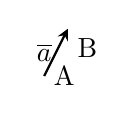
\begin{tikzpicture}[scale=0.3]  % vector image
    	\draw[-stealth, thick] (1,0) -- (2,2);
    	\draw (1,0) node[right]{A};
    	\draw (2,2) node[below right]{B};
    	\draw (1,1) node{$\overline{a}$};
    \end{tikzpicture}
    \caption{Зображення вектора}
    \label{fig:alg:vector-image}
\end{figure}

Вважаємо, що два \textbf{вектори рівні}, якщо їх довжини і напрямки співпадають \ref{fig:alg:colinear-vectors-image}.
Іншими словами, $\overline{a} = \overline{b} \Leftrightarrow \overline{a} \upuparrows \overline{b}$ (напрямки співпадають
та $|\overline{a}| = |\overline{b}|$ (довжини співпадають).

\begin{figure}[ht]
    \centering
    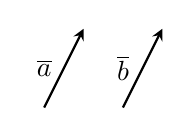
\begin{tikzpicture}[scale=0.5]
        \draw[-stealth, thick] (1,0) -- (2,2);
        \draw (1,1) node{$\overline{a}$};
        \draw[-stealth, thick] (3,0) -- (4,2);
        \draw (3,1) node{$\overline{b}$};
    \end{tikzpicture}
    \caption{Зображення колінеарних векторів}
    \label{fig:alg:colinear-vectors-image}
\end{figure}



\begin{definition}[Колінеарні вектори]
    \textbf{Колінеарні вектори} (паралельні вектори) $(\overline{a} \parallel \overline{b})$
    -- це вектори $\overline{a}$ і $\overline{b}$, які лежать на одній прямій або на паралельних прямих.
\end{definition}

Серед них будемо розрізняти вектори одного напрямку: $\overline{a} \upuparrows \overline{b}$, та протилежного напрямку: $\overline{a} \uparrow \downarrow \overline{b}$.

\begin{definition}[Нульовий вектор]
    \textbf{Нульовий вектор} (нуль - вектор) – це вектор нульової довжини, тобто вектор, кінець і початок якого співпадають, $|\overline{0}| = 0$. Буде зручно вважати нульовий вектор вектором довільного напрямку, тобто нульовий вектор є колінеарним будь-якому вектору.
\end{definition}

\begin{definition}[Протилежні вектори]
    Вектор $\overline{a}'$ -- \textbf{протилежний вектор} до вектора $\overline{a}$ , якщо $\overline{a}' \uparrow \downarrow \overline{a}$ і $|\overline{a}'| = |\overline{a}|$, тобто $\overline{a}' = -\overline{a}$.
\end{definition}

\begin{definition}[Компланарні вектори]
	Вектори $\overline{a}, \overline{b}, \overline{c}, ...$ -- це \textbf{компланарні вектори}, якщо вони лежать в одній площині або паралельні одній площині.
\end{definition}

\subsection{Лінійні операції над векторами}

\subsubsection*{Множення вектора на скаляр}

\begin{definition}[Добуток векторів]
	\textbf{Добуток} вектора $\overline{a} \neq \overline{0}$  і числа $\alpha \in \mathbb{R}$, ($\alpha \overline{a}$) -- це вектор $\overline{b} = \alpha \overline{a}$, який задовольняє такі умови:
		\begin{enumerate}[label=\arabic*)]
			\item $\overline{b}$ колінеарний вектору $\overline{a}$
			\item $|\overline{b}| = |\alpha| |\overline{a}|$
			\item $\overline{b} \upuparrows \overline{a}$ -- однаково направлені, якщо $\alpha > 0$, і $\overline{b} \uparrow \downarrow \overline{a}$ – протилежно направлені, якщо $\alpha < 0$.
		\end{enumerate}
\end{definition}

\subsubsection*{Додавання векторів}

\begin{definition}[Сума векторів]
	\textbf{Сума векторів} $\overline{a}$ і $\overline{b}$, ($\overline{a} + \overline{b}$) -- це вектор, який з’єднує початок вектора $\overline{a}$ з кінцем вектора $\overline{b}$ за умови, що вектор $\overline{b}$ відкладено від кінця вектора $\overline{a}$.
\end{definition}

Цей спосіб додавання векторів -- це \textbf{правило трикутника}.

Два вектори можна додати і за іншим правилом, яке має назву -- \textbf{правило паралелограма}:
сумою двох векторів $\overline{a}$ і $\overline{b}$, відкладених від спільного початку, є
вектор, який збігається з діагоналлю паралелограма, побудованого на векторах $\overline{a}$
і $\overline{b}$ як на сторонах. Початки векторів $\overline{a}$, $\overline{b}$ та
$\overline{a} + \overline{b}$ співпадають.

\begin{figure}[ht]
    \centering
    \begin{tikzpicture}[scale=0.5]  % vector a
        \draw[-stealth, thick] (0,1) -- (1,3);
        \draw (0,2) node{$\overline{a}$};
        \draw[-stealth, thick] (2,2) -- (4,2);
        \draw (3,3) node{$\overline{b}$};
        \draw (1.5,-1) node{Два довільні};
        \draw (1.5,-2) node{вектори};
    \end{tikzpicture}
    \begin{tikzpicture}[scale=0.5]  %triangle rule
        \draw[-stealth, thick] (0,0) -- (1,2);
        \draw (0,1) node{$\overline{a}$};
        \draw[-stealth, thick] (1,2) -- (3,2);
        \draw (2,2.5) node{$\overline{b}$};
        \draw[-stealth, dashed, thick] (0,0) -- (3,2);
        \draw (2,0.5) node{$\overline{a} + \overline{b}$};
        \draw (1.5,-1) node{Правило};
        \draw (1.5,-2) node{трикутника};
    \end{tikzpicture}
    \begin{tikzpicture}[scale=0.5]  % paralelogram rule
        \draw[-stealth, thick] (0,0) -- (1,2);
        \draw (0,1) node{$\overline{a}$};
        \draw[-stealth, thick] (0,0) -- (2,0);
        \draw (1.5,0.5) node{$\overline{b}$};
        \draw[-stealth, thick] (0,0) -- (3,2);
        \draw (4,2) node{$\overline{a} + \overline{b}$};
        \draw[-stealth, dashed, thick] (1,2) -- (3,2);
        \draw[-stealth, dashed, thick] (2,0) -- (3,2);
        \draw (2,-1) node{Правило};
        \draw (2,-2) node{паралелограма};
    \end{tikzpicture}
    \caption{Правила додавання}
    \label{fig:alg:vector-addition-rules}
\end{figure}

Використовуючи послідовно правило трикутника, можна побудувати суму скінченної
кількості довільних векторів \ref{fig:alg:zero-vector-sum}. Якщо кінець останнього вектора співпадає з
початком першого, то сумою векторів є нульовий вектор: $\overline{0}$.

\begin{figure}[ht]
    \centering
    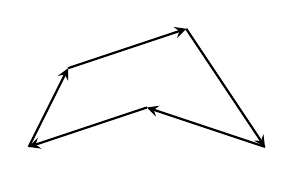
\begin{tikzpicture}[scale=0.5]  %triangle rule
        \draw[-stealth, thick] (0,0) -- (1,2);
        \draw[-stealth, thick] (1,2) -- (4,3);
        \draw[-stealth, thick] (4,3) -- (6,0);
        \draw[-stealth, thick] (6,0) -- (3,1);
        \draw[-stealth, thick] (3,1) -- (0,0);
    \end{tikzpicture}
    \caption{Вектори, сума яких -- це нульовий вектор.}
    \label{fig:alg:zero-vector-sum}
\end{figure}

\subsection*{Віднімання векторів}
 
\begin{definition}[Різниця векторів]
	\textbf{Різниця векторів} $\overline{a}$ і $\overline{b}$, ($\overline{a} - \overline{b}$) -- це вектор $\overline{c}$, який в сумі з вектором $\overline{b}$ дає вектор $\overline{a}$ , тобто $\overline{b} + \overline{c} = \overline{a}$. 
\end{definition}

Очевидно, що $\overline{c} = \overline{a} + (-\overline{b})$.

\begin{center}
	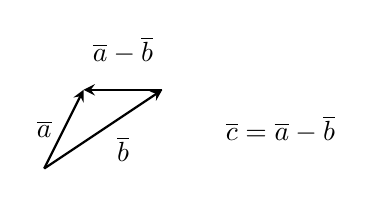
\begin{tikzpicture}[scale=0.5]  % paralelogram rule
		\draw[-stealth, thick] (0,0) -- (1,2);
		\draw (0,1) node{$\overline{a}$};
		\draw[-stealth, thick] (3,2) -- (1,2);
		\draw (2,3) node{$\overline{a} - \overline{b}$};
		\draw[-stealth, thick] (0,0) -- (3,2);
		\draw (2,0.5) node{$\overline{b}$};
		\draw (6,1) node{$\overline{c} = \overline{a} - \overline{b}$};
	\end{tikzpicture}
\end{center}

\subsection{Властивості лінійних операцій, аксіоми векторної алгебри}

\begin{enumerate}
	\item $(\alpha \beta) \overline{a} = \alpha (\beta \overline{a})$ -- асоціативність відносно множення на скаляр.

 	\item $\overline{a} + \overline{b} = \overline{b} + \overline{a}$ -- комутативність додавання.

 	\item $(\overline{a} + \overline{b}) + \overline{c} = \overline{a} + (\overline{b} + \overline{c})$ -- асоціативність додавання.
	
	\item \parbox[t]{8cm}{
		$\left.\begin{array}{l}
			(\alpha + \beta)\overline{a} = \alpha\overline{a} + \beta\overline{a}  \\
			\overline{a}(\alpha + \beta) = \overline{a}\alpha + \overline{a}\beta
		\end{array} \right\}$ -- дистрибутивність.
	}
	
	\item $\exists! \overline{0}: \forall\overline{a}: \overline{a} + \overline{0} = \overline{a}$ -- існування єдиного нуля.
    
    \item $\forall\overline{a} \exists!\overline{a}': \overline{a}' + \overline{a} = \overline{0}$ -- існування протилежного вектора.
    
    \item $1\cdot\overline{a} = \overline{a}$    
\end{enumerate}

\subsection{Базис на прямій, на площині, у просторі}

Розглянемо множину векторів, колінеарних вектору $\overline{a} \neq \overline{0}$. Позначимо її $E^1$.

Нехай $\overline{a}, \overline{b}, \overline{c} \in E^1$.

\begin{center}
	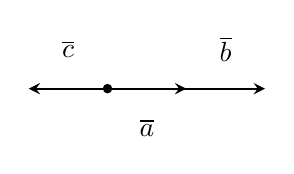
\begin{tikzpicture}[scale=0.5]
		\draw[-stealth, thick] (2,0) -- (0,0);
		\draw (1,1) node{$\overline{c}$};
		\filldraw[black] (2,0) circle (3pt);
		\draw[-stealth, thick] (2,0) -- (4,0);
		\draw (3,-1) node{$\overline{a}$};
		\draw[-stealth, thick] (2,0) -- (6,0);
		\draw (5,1) node{$\overline{b}$};
	\end{tikzpicture}
\end{center}

\begin{theorem} \label{vectorSingleRepresentation}
	$\forall \overline{b} \in E^1 \exists$ дійсне число $\alpha$ таке, що $\overline{b} = \alpha\overline{a}$, причому це представлення єдине. 
\end{theorem}
\begin{proof}
	Доведемо єдиність даного представлення методом від супротивного.
	
	Нехай $\overline{b} = \tilde{\alpha}\overline{a}$
	
	Тоді $\overline{0} = \overline{b} - \overline{b} = \tilde{\alpha}\overline{a} - \alpha\overline{a} = (\tilde{\alpha} - \alpha)\overline{a} \Rightarrow \tilde{\alpha} - \alpha = 0 \Rightarrow \tilde{\alpha} = \alpha$ 

	Вкажемо значення коефіцієнта $\alpha$.
	
	Якщо $\overline{a} \upuparrows \overline{b}$, то $\alpha = \dfrac{|\overline{b}|}{|\overline{a}|}$.
	
	Дійсно: $|\alpha\overline{a}| = \left|\dfrac{|\overline{b}|}{|\overline{a}|}\right||\overline{a}| = \dfrac{|\overline{b}|}{|\overline{a}|}|\overline{a}| = |\overline{b}|$, $\alpha\overline{a} \upuparrows \overline{b}$.

	Якщо ж $\overline{a} \uparrow \downarrow \overline{b}$, то $\alpha = -\dfrac{|\overline{b}|}{|\overline{a}|}$ (доведення аналогічне).
\end{proof}

Нехай $\overline{a} \nparallel \overline{b}$ ( тому $\overline{a} \neq \overline{0}$, $\overline{b} \neq \overline{0}$). Розглянемо множину векторів, компланарних векторам $\overline{a}$ та $\overline{b}$, позначимо її $E^2$.
Нехай $\overline{a}, \overline{b}, \overline{c} \in E^2$.

\begin{theorem}
	$\forall \overline{c} \in E^2 ~ \exists!$  дійсні $\alpha, \beta$, такі, що $\overline{c} = \alpha\overline{a} + \beta\overline{b}$.
\end{theorem} 

\begin{proof}
    Проведемо доведення графічно. 
    
    % \begin{wrapfigure}{r}{4cm}
    \begin{center}
        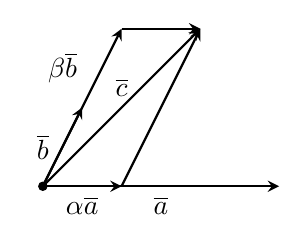
\begin{tikzpicture}[scale=0.5]
            \draw[-stealth, thick] (0,0) -- (1,2);
            \draw[-stealth, thick] (0,0) -- (2,4);
            \draw[-stealth, thick] (0,0) -- (2,0);
            \draw[-stealth, thick] (2,4) -- (4,4);
            \draw[-stealth, thick] (0,0) -- (4,4);
            \draw[-stealth, thick] (2,0) -- (4,4);
            \draw[-stealth, thick] (0,0) -- (6,0);
            \draw (0,1) node{$\overline{b}$};
            \draw (0.5,3) node{$\beta\overline{b}$};
            \draw (1,-0.5) node{$\alpha\overline{a}$};
            \draw (3,-0.5) node{$\overline{a}$};
            \draw (2,2.5) node{$\overline{c}$};
            \filldraw[black] (0,0) circle (3pt);
        \end{tikzpicture}
    \end{center}
    % \end{wrapfigure}
	
    З кінця вектору $\overline{c}$ проведемо дві прямі паралельно векторам $\overline{a}$
    і $\overline{b}$ відповідно до перетину з цими векторами чи прямими, на яких вони лежать. 
    Отримали паралелограм, дві сторони якого дорівнюють відповідно $\alpha\overline{a}$ і
    $\beta\overline{b}$ (за теоремою~\ref{vectorSingleRepresentation}).
    Діагоналлю цього паралелограма є вектор $\overline{c}$, тобто $\overline{c} = \alpha\overline{a} + \beta\overline{b}$.
    Єдиність коефіцієнтів $\alpha$ та $\beta$ випливає з двох умов: 
    \begin{enumerate}
        \item Існує лише одна точка перетину непаралельних прямих, 
        \item за теоремою~\ref{vectorSingleRepresentation} константи $\alpha$ і $\beta$ визначаються однозначно.
    \end{enumerate}
\end{proof}

Нехай $E^3$ -- множина всіх векторів у просторі, причому $\overline{a}, \overline{b}, \overline{c}$ -- некомпланарні $(\overline{a} \neq \overline{0}, \overline{b} \neq \overline{0}, \overline{c} \neq \overline{0})$.

\begin{theorem}
	$\forall\overline{d}\in E^3, \exists! ~ \alpha, \beta, \gamma : \overline{d} = \alpha\overline{a} + \beta\overline{b} + \gamma\overline{c}$.
\end{theorem}
\begin{proof}
    % \begin{wrapfigure}{l}{4.2cm}
    \begin{center}
        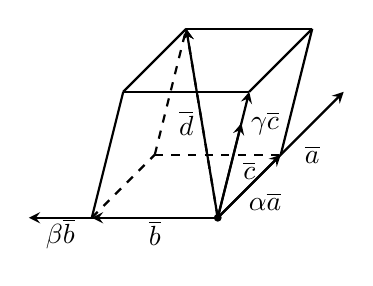
\begin{tikzpicture}[scale=0.4]
            \draw[-stealth, thick] (6,1) -- (2,1);
            \draw[-stealth, thick] (6,1) -- (0,1);
            \draw[-stealth, thick] (6,1) -- (5,7);
            \draw[-stealth, thick] (6,1) -- (6.75,4);
            \draw[-stealth, thick] (6,1) -- (7,5);
            \draw[-stealth, thick] (6,1) -- (8,3);
            \draw[-stealth, thick] (6,1) -- (10,5);
                    
            \draw[thick] (2,1) -- (3,5);
            \draw[thick] (3,5) -- (5,7);
            \draw[thick] (3,5) -- (7,5);
            \draw[thick] (5,7) -- (9,7);
            \draw[thick] (7,5) -- (9,7);
            \draw[thick] (8,3) -- (9,7);
        
            \draw[thick, dashed] (2,1) -- (4,3);
            \draw[thick, dashed] (4,3) -- (5,7);
            \draw[thick, dashed] (4,3) -- (8,3);
            \draw[-stealth, dashed, thick] (6,1) -- (5,7);
            
            \draw (1,0.5) node{$\beta\overline{b}$};
            \draw (4,0.5) node{$\overline{b}$};
            \draw (5,4) node{$\overline{d}$};
            \draw (7,2.5) node{$\overline{c}$};
            \draw (7.5,4) node{$\gamma\overline{c}$};
            \draw (7.5,1.5) node{$\alpha\overline{a}$};
            \draw (9,3) node{$\overline{a}$};
            \filldraw[black] (6,1) circle (3pt);
        \end{tikzpicture}
    \end{center}
    % \end{wrapfigure}
    Із кінця вектора $\overline{d}$ проведемо три площини, паралельні парам
    векторів $(\overline{b}, \overline{c})$, $(\overline{a}, \overline{c})$, $(\overline{a}, \overline{b})$.
    Ці площини перетнуть прямі, на яких лежать $\overline{a}, \overline{b}, \overline{c}$ в
    єдиних точках.
    За теоремою~\ref{vectorSingleRepresentation} отримаємо нові вектори
    $\alpha\overline{a}, \beta\overline{b}, \gamma\overline{c}$, а вектор $\overline{d}$ – це діагональ
    паралелепіпеда, на них побудованого, тобто
    $\overline{d} = \alpha\overline{a} + \beta\overline{b} + \gamma\overline{c}$, що і треба було довести.
\end{proof}

\begin{remark}
    Базисом у множині $E^1$ може слугувати довільний ненульовий
    вектор, базисом у $E^2$ – впорядкована пара неколінеарних векторів, а в $E^3$ ---
    впорядкована трійка некомпланарних векторів. Вектору $\overline{b}$ було поставлено у
    відповідність число $\alpha$; вектору $\overline{c}$ – числа $\alpha$ і $\beta$; вектору 
    $\overline{d}$ – числа $\alpha, \beta, \gamma$. 
    Ці числа називаються -- коефіцієнти розкладу векторів $\overline{b}, \overline{c}, \overline{d}$ за базисами
    $\overline{a}$; $\overline{a}, \overline{b}$; $\overline{a}, \overline{b}, \overline{c}$ просторів $E^1, E^2$ і $E^3$ відповідно.
\end{remark}

\begin{definition}[Розклад Вектора за базисом]
    \textbf{Коефіцієнти розкладу вектора $\overline{a}$ за базисом $\overline{a}_1, \overline{a}_2, ...$}
    -- це числа $\alpha_1, \alpha_2, ... \in \mathbb{R}$, такі, що
    $\overline{a} = \alpha_1\overline{a}_1 + \alpha_2\overline{a}_2 + ...$.
\end{definition}

\subsection{Декартів прямокутний базис}

\begin{definition}[Права трійка векторів]
    Впорядкована трійка некомпланарних векторів $(\overline{a}, \overline{b}, \overline{c})$ називається правою (\textbf{права трійка векторів}),
    якщо з кінця вектора $\overline{c}$ поворот від $\overline{a}$ до $\overline{b}$, менший за $180^{\circ}$, тобто відбувається проти
    годинникової стрілки.
\end{definition}

\begin{definition}[Декартів правий прямокутний базис]
    Трійка векторів $\overline{i}, \overline{j}, \overline{k}$ утворює \textbf{декартів правий прямокутний базис},
    якщо: 
    \begin{enumerate}
        \item $\overline{i} \perp \overline{j}, \overline{j} \perp \overline{k}, \overline{k} \perp \overline{i}$
        \item $|\overline{i}| = |\overline{j}| = |\overline{k}| = 1$
        \item $\overline{i}, \overline{j}, \overline{k}$ -- права трійка
    \end{enumerate}
\end{definition}

\subsection{Проекція вектора на вектор (або на вісь)}

Нехай задано $\overline{a} \neq \overline{0}$.

\begin{definition}[Проекція вектора на вектор]
    \textbf{Проекція вектора $\overline{AB}$ на вектор $\overline{a}$} називається довжина відрізка
    $A'B'$ між основами перпендикулярів, опущених з точок A та B на вектор $\overline{a}$ (або напряму,
    на якій він лежить): 
\end{definition}

\begin{center}
	\parbox{4cm}{
		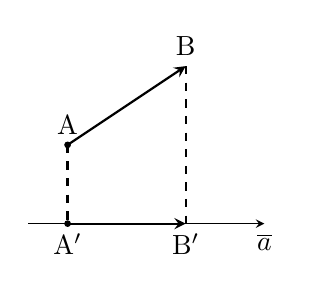
\begin{tikzpicture}[scale=0.5]
			\draw[-stealth] (0,0) -- (6,0)node[below]{$\overline{a}$};
			\draw[-stealth, thick] (1,2)node[above]{A} -- (4,4)node[above]{B};
			\filldraw[black] (1,2) circle (2pt);
			\draw[-stealth, thick] (1,0)node[below]{A$'$} -- (4,0)node[below]{B$'$};
			\filldraw[black] (1,0) circle (2pt);	
			\draw[dashed, thick] (1,2) -- (1,0);
			\draw[dashed, thick] (4,4) -- (4,0);
		\end{tikzpicture}
	}
	\parbox{6.2cm}{
		$\text{пр}_{\overline{a}}\overline{AB} = \left\{ \begin{array}{l}
			|\overline{A'B'}| \text{, якщо } \overline{A'B'}\uparrow\uparrow \overline{a}  \\
			-|\overline{A'B'}|\text{, якщо } \overline{A'B'}\uparrow\downarrow\overline{a}  \\
		\end{array}\right.$
	}
\end{center}

\subsection*{Властивості проекції:}
\begin{enumerate}
	\item $\text{пр}_{\overline{a}}\alpha\overline{b} = \alpha\text{пр}_{\overline{a}}\overline{b}$
	\item $\text{пр}_{\overline{a}}(\overline{a} + \overline{b}) = \text{пр}_{\overline{a}}\overline{a} + \text{пр}_{\overline{a}}\overline{b}$
\end{enumerate}

\subsection{Множення векторів. Скалярний добуток двох векторів}

\begin{definition}[Скалярний добуток]
	\textbf{Скалярний добуток} векторів $\overline{a}$ і $\overline{b}$ (позначається
	$\overline{a}\cdot\overline{b}$, $\overline{a}\overline{b}$ чи $(\overline{a}, \overline{b})$)
	--- це число, яке дорівнює добутку довжин цих векторів на косинус кута між ними: 
	$(\overline{a}, \overline{b}) = |\overline{a}||\overline{b}|\cos\varphi$, де
	$\varphi = \widehat{(\overline{a}, \overline{b})}$.
\end{definition}

\subsection*{Алгебраїчні властивості скалярного добутку:}
\begin{enumerate}
	\item $(\overline{a}, \overline{b}) = (\overline{b}, \overline{a})$ -- комутативність.
	\item $\left.\begin{array}{l}
				(\alpha\overline{a}, \overline{b}) = \alpha(\overline{a}, \overline{b}) = (\overline{a}, \alpha\overline{b})  \\
				(\overline{a} + \overline{a}', \overline{b}) = (\overline{a}, \overline{b}) + (\overline{a}', \overline{b})  \\
				(\overline{a}, \overline{b} + \overline{b}') = (\overline{a}, \overline{b}) + (\overline{a}, \overline{b}')  \\
		  \end{array}\right\}$ -- лінійність.
\end{enumerate}

\subsection*{Геометричні властивості скалярного добутку:}
\begin{enumerate}
	\item $(\overline{a}, \overline{b}) = 0 \Leftrightarrow \overline{a} \perp \overline{b}$.
	\item $(\overline{a}, \overline{a}) = |\overline{a}|^2 \Rightarrow |\overline{a}| = \sqrt{(\overline{a}, \overline{a})}$.
\end{enumerate}

\subsection{Скалярний добуток в координатах}

Нехай $\{\overline{e}_1, \overline{e}_2, \overline{e}_3\}$ – це фіксований базис в просторі $E^3$,
$\overline{x}, \overline{y} \in E^3$. Тоді:
\begin{center}
	$\overline{x} = x_1\overline{e}_1 + x_2\overline{e}_2 + x_3\overline{e}_3$  \\
	$\overline{y} = y_1\overline{e}_1 + y_2\overline{e}_2 + y_3\overline{e}_3$  \\
\end{center}

Обчислимо скалярний добуток цих векторів: 

\begin{equation*}
    \begin{split}
        (\overline{x}, \overline{y})
        & = (x_1\overline{e}_1 + x_2\overline{e}_2 + x_3\overline{e}_3, \overline{y})\\
        & = (x_1 \overline{e}_1, \overline{y}) + (x_2 \overline{e}_2, \overline{y})
        + (x_3 \overline{e}_3, \overline{y})\\
        & = x_1(\overline{e}_1, y_1\overline{e}_1 + y_2\overline{e}_2 + y_3\overline{e}_3)\\
        & \quad + x_2(\overline{e}_2, y_1\overline{e}_1 + y_2\overline{e}_2 + y_3\overline{e}_3)\\
        & \quad+ x_3(\overline{e}_3, y_1\overline{e}_1 + y_2\overline{e}_2 + y_3\overline{e}_3)\\
        & = x_1 y_1(\overline{e}_1, \overline{e}_1)
        + x_1 y_2(\overline{e}_1, \overline{e}_2)
        + x_1 y_3(\overline{e}_1, \overline{e}_3)\\
        & \quad+ x_2 y_1(\overline{e}_2, \overline{e}_1)
        + x_2 y_2(\overline{e}_2, \overline{e}_2)
        + x_2 y_3(\overline{e}_2, \overline{e}_3)\\
        & \quad+ x_3 y_1(\overline{e}_3, \overline{e}_1)
        + x_3 y_2(\overline{e}_3, \overline{e}_2)
        + x_3 y_3(\overline{e}_3, \overline{e}_3)\\
        & = x_1 y_1(\overline{e}_1, \overline{e}_1)
        + (x_1 y_2 + x_2 y_1)(\overline{e}_1, \overline{e}_2)
        + (x_1 y_3 + x_3 y_1)(\overline{e}_1, \overline{e}_3)\\
        & \quad+ x_2 y_2(\overline{e}_2, \overline{e}_2)
        + (x_2 y_3 + x_3 y_2)(\overline{e}_2, \overline{e}_3)
        + x_3 y_3(\overline{e}_3, \overline{e}_3).\\
    \end{split}    
\end{equation*}

У частковому випадку, коли $\overline{e}_1 = \overline{i}, \overline{e}_2 = \overline{j}, \overline{e}_3 = \overline{k}$, маємо: 
$(\overline{e}_1, \overline{e}_2) = (\overline{e}_2, \overline{e}_3) = (\overline{e}_3, \overline{e}_1)$, $(\overline{e}_i, \overline{e}_j) = 1$, де $i = 1, 2, 3$.А отже

\begin{equation*}
    (\overline{x}, \overline{y}) = x_1 y_1 + x_2 y_2 + x_3 y_3.
\end{equation*}

Якщо $\overline{a} = (x, y, z)$, то $|\overline{a}| = \sqrt{(\overline{a}, \overline{a})} = \sqrt{x^2 + y^2 + z^2}$.

\subsection{Нормування вектора}

\begin{definition}[Орт-вектор]
	Нехай $\overline{a} \neq \overline{0}$. \textbf{Орт-вектор} вектора $\overline{a}$ -- це вектор $\overline{a}_o$, такий, що $\overline{a}_o \uparrow\uparrow \overline{a}$ і $|\overline{a}_o| = 1$. 
\end{definition}

\begin{definition}[Нормування вектора]
	 \textbf{Нормування вектора} $\overline{a}$ -- це процес отримання орт-вектора $\overline{a}_o$, $\overline{a}_o = \dfrac{1}{|\overline{a}|}\overline{a}$
\end{definition}

Якщо $\overline{a} = (x, y, z)$, то
$$\overline{a}_o = \left(\dfrac{x}{\sqrt{x^2+y^2+z^2}}, \dfrac{y}{\sqrt{x^2+y^2+z^2}}, \dfrac{z}{\sqrt{x^2+y^2+z^2}} \right).$$

Геометричний сенс координат орт-вектора $\overline{a}_o$ у декартовій системі координат:
\begin{equation*}
    \overline{a}_o = (\cos\alpha, \cos\beta, \cos\gamma),
\end{equation*}
де,
\begin{equation*}    
    \alpha = \widehat{(\overline{a}, OX)} = \widehat{(\overline{a}_o, OX)},\\
    \beta = \widehat{(\overline{a}, OY)} = \widehat{(\overline{a}_o, OY)},\\
    \gamma = \widehat{(\overline{a}, OZ)} = \widehat{(\overline{a}_o, OZ)}.
\end{equation*}

\begin{definition}[Напрямні косинуси]
	Косинуси кутів, які утворює вектор (або його орт) з осями координат -- це \textbf{напрямні косинуси}.
\end{definition}

Знайдемо косинус кута $\alpha$: 
$$\cos\alpha = \dfrac{(\overline{a}, \overline{i})}{|\overline{a}||\overline{i}|} = \dfrac{x}{\sqrt{x^2+y^2+z^2}}$$

\begin{claim}
	$\cos^2\alpha + \cos^2\beta + \cos^2\gamma = 1$.
\end{claim}

Формула для довжини проекції вектора:
$$x = |\overline{a}|\cos\alpha = \text{пр}_{\overline{i}}\overline{a}$$

\subsection{Векторний добуток двох векторів}

\begin{definition}[Векторний добуток]
	\textbf{Векторний добуток} векторів $\overline{a}$ і $\overline{b}$ $[\overline{a}, \overline{b}]$
	--- це вектор $\overline{c}$, що задовольняє умови:
	\begin{enumerate}
		\item $\overline{c}\perp\overline{a}$, $\overline{c}\perp\overline{b}$
		\item $|\overline{a}| = |\overline{a}||\overline{b}|\sin\varphi$, $\varphi = (\widehat{\overline{a},
			\overline{b}})$
		\item $\overline{a}$, $\overline{b}$, $\overline{c}$ -- права трійка
	\end{enumerate}
\end{definition}

\begin{remark}
	Оскільки $\overline{c}\perp\overline{a}$, $\overline{c}\perp\overline{b}$, то $\overline{c}$
	перпендикулярний площині векторів $\overline{a}$ і $\overline{b}$. 
\end{remark}

\subsection*{Алгебраїчні властивості векторного добутку:}

1) $[\overline{a}, \overline{b}] = - [\overline{b}, \overline{a}]$
	
2) $[\alpha\overline{a}, \overline{b}] = \alpha[\overline{a}, \overline{b}] = [\overline{a}, \alpha\overline{b}]$

3) $[\overline{a} + \overline{b}, \overline{c}] = [\overline{a}, \overline{c}] + [\overline{b}, \overline{c}]$
	
4) $[\overline{a}, \overline{b} + \overline{c}] = [\overline{a}, \overline{b}] + [\overline{a}, \overline{c}]$

\textit{Доведення:}

\begin{proof}
	1) Нехай $[\overline{a}, \overline{b}] = \overline{c}$, $[\overline{b}, \overline{a}] = \overline{d}$.
	Тоді: $\overline{c} \perp \overline{a}$ і $\overline{c} \perp \overline{b}$,
	$\overline{d} \perp \overline{b}$ і $\overline{d} \perp \overline{a}$, тобто вектори $\overline{c}$
	і $\overline{d}$ перпендикулярні до площини, в якій лежать вектори $\overline{a}$ і $\overline{b}$,
	отже, $\overline{c} \parallel \overline{d}$.
	
	$|\overline{c}| = |\overline{a}||\overline{b}|\sin\varphi = |\overline{d}|$, де
	$\varphi = (\widehat{\overline{a},\overline{b}})$.
	
	$\overline{a}$, $\overline{b}$, $\overline{c}$ -- права трійка; $\overline{b}$, $\overline{a}$,
	$\overline{d}$ -- також права трійка $\Rightarrow$ $\overline{a}$, $\overline{b}$, $\overline{d}$
	--- ліва трійка, тому вектори $\overline{c}$ та $\overline{d}$ протилежно направлені.
	
	Отже, вектори $\overline{c}$ та $\overline{d}$ колінеарні, мають однакову довжину та протилежно
	направлені. Тому $\overline{c} = -\overline{d}$.

	~	
	
	2) Якщо $\alpha = 0$ або $\overline{a} \parallel \overline{b}$, то рівності очевидні: 
	$[\alpha \overline{a}, \overline{b}] = \alpha [\overline{a}, \overline{b}] = \overline{0}$.
	Нехай $\alpha < 0$, $[\overline{a}, \overline{b}] = \overline{c}$,
	$\varphi = (\widehat{\overline{a}, \overline{b}})$, $[\alpha \overline{a}, \overline{b}] = \overline{d}$.
	Тоді:
	
	$|\alpha \overline{c}| = |\alpha [\overline{a}, \overline{b}]| = |\alpha| |[\overline{a}, \overline{b}]|
	= -\alpha |\overline{a}| |\overline{b}| \sin\varphi$.
	
	$|[\alpha \overline{a}, \overline{b}]|
	= |\alpha \overline{a}| |\overline{b}]|\sin(\widehat{\alpha \overline{a},\overline{b}})
	= |\alpha| |\overline{a}| |\overline{b}]|\sin(\pi - \varphi)
	= -\alpha |\overline{a}| |\overline{b}]| \sin\varphi$.
	
	$\overline{c}\perp$ площині, в якій лежать $\overline{a}$ і $\overline{b}$
	$\Rightarrow \overline{c} \perp$ площині, в якій лежать $\alpha \overline{a}$ і $\overline{b}$.
	
	$\overline{d}\perp$ площині, в якій лежать $\alpha \overline{a}$ і $\overline{b}$, отже,
	$\overline{c} \parallel \overline{d}$.
	
	$\overline{a}$, $\overline{b}$, $\overline{c}$ -- права трійка $\alpha \overline{a}$,
	$\overline{b}$, $\overline{c}$ -- ліва трійка, $\overline{a}$, $\overline{b}$,
	$\alpha \overline{c}$ -- ліва трійка.
	
	$\alpha \overline{a}$, $\overline{b}$, $\overline{d}$ -- права трійка $\overline{a}$,
	$\overline{b}$, $\overline{d}$ -- ліва трійка; отже, вектори $\alpha \overline{c}$ та $\overline{d}$.
	однаково направлені.
	
	Враховуючи однакову довжину векторів $\alpha \overline{c}$ та $\overline{d}$, маємо
	$\alpha \overline{c} = \overline{d}$ або $[\alpha \overline{a}, \overline{b}]
	= \alpha [\overline{a}, \overline{b}]$.

	~

	3), 4) -- очевидно.
\end{proof}

\subsection*{Геометричні властивості векторного добутку:}

1) $[\overline{a}, \overline{b}] = \overline{0} \Leftrightarrow \overline{a} \parallel \overline{b}$

2) $|[\overline{a}, \overline{b}]| = S_{\Diamond \overline{a}\overline{b}}$, де
$S_{\Diamond \overline{a}\overline{b}}$ -- площа паралелограма, побудованого на векторах
$\overline{a}$ та $\overline{b}$ , як на сторонах

\textit{Доведення:}

\begin{proof}
	1) $|[\overline{a},\overline{b}]| = |\overline{a}| |\overline{b}| \sin\varphi = 0
	\Rightarrow \overline{a} = \overline{0}$ або $\overline{b} = \overline{0}$, або $\sin \varphi = 0
	\Rightarrow \overline{a} \parallel \overline{b}$.
	
	Якщо $\overline{a} \parallel \overline{b}$, то $\sin \varphi = 0$, і $|[\overline{a}, \overline{b}]| = 0
	\Rightarrow [\overline{a}, \overline{b}] = \overline{0}$.
	
	~	
	
	2) $|[\overline{a},\overline{b}]| = |\overline{a}| |\overline{b}| \sin \varphi = |\overline{a}| h
	= S_{\Diamond \overline{a}\overline{b}}$.
\end{proof}

\begin{claim}
	$[\overline{a}, \overline{a}] = 0$.
\end{claim}

\subsection{Векторний добуток в координатах}

Нехай в просторі $E^3$ зафіксовано базис $\{\overline{i}, \overline{j}, \overline{k}\}$, $\overline{x}, \overline{y} \in E^3$, тоді 

$$\overline{x} = x_1\overline{i} + y_1\overline{j} + z_1\overline{k}$$

$$\overline{y} = x_2\overline{i} + y_2\overline{j} + z_2\overline{k}$$

Знайдемо координати вектору $[\overline{x}, \overline{y}]$.

Зауважимо, що $[\overline{i}, \overline{j}] = \overline{k}$, $[\overline{j}, \overline{k}] = \overline{i}$,
$[\overline{k}, \overline{i}] = \overline{j}$. Тоді:

\noindent$[\overline{i}, \overline{j}]
= [x_1\overline{i} + y_1\overline{j} + z_1\overline{k}
	, x_2\overline{i} + y_2\overline{j} + z_2\overline{k}]
= x_1 x_2[\overline{i},\overline{i}]
	+ x_1 y_2[\overline{i},\overline{j}]
	+ x_1 z_2[\overline{i},\overline{k}]
	+ y_1 x_2[\overline{j},\overline{i}]
	+ y_1 y_2[\overline{j},\overline{j}]
	+ y_1 z_2[\overline{j},\overline{k}]
	+ z_1 x_2[\overline{k},\overline{i}]
	+ z_1 y_2[\overline{k},\overline{j}]
	+ z_1 z_2[\overline{k},\overline{k}]
= (x_1 y_2 - x_2 y_1)[\overline{i},\overline{j}]
	+ (x_1 z_2 - x_2 z_1)[\overline{i},\overline{k}]
	+ (y_1 z_2 - y_2 z_1)[\overline{j},\overline{k}]
= (x_1 y_2 - x_2 y_1)\overline{k}
	+ (x_1 z_2 - x_2 z_1)\overline{j}
	+ (y_1 z_2 - y_2 z_1)\overline{i}
= (y_1 z_2 - y_2 z_1)\overline{i}
	+ (x_1 z_2 - x_2 z_1)\overline{j}
	+ (x_1 y_2 - x_2 y_1)\overline{k}.$

\begin{problem}[Знайти площу трикутника]
    Знайти площу трикутника з вершинами
    \begin{equation*}
        A(3, 0, -1), B(-2, 4, 1), C(2, 1, -3).
    \end{equation*}
\end{problem}
\begin{solution}
    $S = \dfrac{1}{2}|[\overline{AB},\overline{AC}]|$. Оскільки
    $\overline{AB} = (-5, 4, 2), \overline{AC} = (-1, 1, -2)$,
    то 
    \begin{equation*}
        [\overline{AB},\overline{AC}] = -10\overline{i} - 12\overline{j} - \overline{k}.
    \end{equation*}
    Тоді
    \begin{equation*}    
        |[\overline{AB},\overline{AC}]|
        = \sqrt{(-10)^2 + (-12)^2 + (-1)^2}
	= \sqrt{100 + 144 + 1} = \sqrt{245},
    \end{equation*}
    а отже, $S = \dfrac{1}{2}\sqrt{245}$.
\end{solution}

\subsection{Мішаний добуток трьох векторів}

\begin{definition}[Мішаний добуток]
	\textbf{Мішаний добуток} векторів $\overline{a}, \overline{b}, \overline{c}$ -- це скалярний добуток $\overline{a}$
	з векторним добутком векторів $\overline{b}$ і $\overline{c}$, тобто $\overline{a}\overline{b}\overline{c} = (\overline{a}, [\overline{b}, \overline{c}])$. 
\end{definition}

\begin{theorem}
	Мішаний добуток векторів $\overline{a}, \overline{b}, \overline{c}$ дорівнює об’єму паралелепіпеда
	$V_{\text{пар}}$, побудованого на цих векторах, якщо вони складають праву трійку i дорівнює
	$-V_{\text{пар}}$, якщо $\overline{a}, \overline{b}, \overline{c}$ – ліва трійка:
	
	$$\overline{a}\overline{b}\overline{c} = \left\{\begin{array}{ll}
		V_{\text{пар}},		& \text{ якщо } \overline{a},\overline{b},\overline{c} \text{ -- права трійка}  \\
		-V_{\text{пар}},	& \text{ якщо } \overline{a},\overline{b},\overline{c} \text{ -- ліва трійка}  \\
	\end{array} \right.$$
\end{theorem}
\begin{proof}
    Розглянемо випадок, коли $\overline{a},\overline{b},\overline{c}$ -- права трійка \ref{fig:alg:scalar-triple-product}.
	
    % \begin{wrapfigure}{l}{4cm}
    
    % \end{wrapfigure}
    
    Нехай $[\overline{b}, \overline{c}] = \overline{d}$. Тоді $\overline{b}$, $\overline{c}$,
    $\overline{d}$ -- права трійка. Позначимо $\varphi = \widehat{(\overline{a}, \overline{d})}$.
    
    Тоді
    \begin{equation*}
        \begin{split}
            \overline{a}\overline{b}\overline{c}
            &= (\overline{a}, [\overline{b},\overline{c}])\\
            &= (\overline{a},\overline{d})\\
            &= |\overline{a}||\overline{d}|\cos\varphi\\
            &= S_{\Diamond \overline{c}\overline{b}}|\overline{a}|\cos\varphi\\
            &= S_{\Diamond \overline{c}\overline{b}}h\\
            &= V_{\text{пар}},\\
        \end{split}
    \end{equation*}
    оскільки висота
    паралелепіпеда $h = |\overline{a}|\sin\left(\dfrac{\pi}{2} - \varphi\right) = |\overline{a}|\cos\varphi$.
    У випадку, коли $\overline{a}, \overline{b}, \overline{c}$ -- ліва трійка, доведення
    аналогічне.
\end{proof}

\begin{figure}[ht]
    \centering
    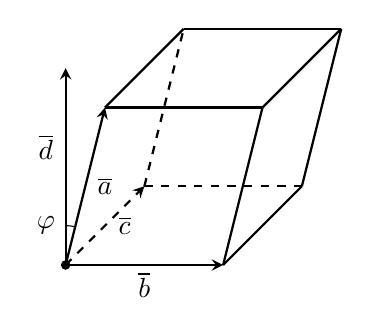
\begin{tikzpicture}[scale=0.5]
        \draw[-stealth, thick] (0,0) -- (0,5);
        \draw[-stealth, thick] (0,0) -- (1,4);
        \draw[-stealth, thick, dashed] (0,0) -- (2,2);
        \draw[-stealth, thick] (0,0) -- (4,0);
                
        \draw[thick] (1,4) -- (5,4);
        \draw[thick] (1,4) -- (3,6);
        \draw[thick] (5,4) -- (7,6);
        \draw[thick] (3,6) -- (7,6);
        \draw[thick] (4,0) -- (6,2);
        \draw[thick] (6,2) -- (7,6);
        \draw[thick] (4,0) -- (5,4);
            
        \draw[thick, dashed] (2,2) -- (3,6);
        \draw[thick, dashed] (2,2) -- (6,2);
                
        \filldraw[black] (0,0) circle (3pt);
                
        \draw (-0.5,3) node{$\overline{d}$};
        \draw (2,-0.5) node{$\overline{b}$};
        \draw (1.5,1) node{$\overline{c}$};
        \draw (1,2) node{$\overline{a}$};
    
        \draw[black] (0,1) arc (90:75.97:1);
        \draw (-0.5,1) node{$\varphi$};
    \end{tikzpicture}
    \caption{Мішаний добуток трьох векторів}
    \label{fig:alg:scalar-triple-product}
\end{figure}

\subsection*{Алгебраїчні властивості:}

\begin{enumerate}
	\item $\overline{a}\overline{b}\overline{c} = \overline{c}\overline{a}\overline{b} = \overline{b}\overline{c}\overline{a} = -\overline{b}\overline{a}\overline{c} = -\overline{c}\overline{b}\overline{a} = -\overline{a}\overline{c}\overline{b}$
	\item $(\alpha\overline{a})\overline{b}\overline{c} = \alpha\overline{a}\overline{b}\overline{c} = \overline{a}(\alpha\overline{b})\overline{c} = \overline{a}\overline{b}(\alpha\overline{c})$
	\item $\begin{array}{l}
			(\overline{a}+\overline{a}')\overline{b}\overline{c} = \overline{a}\overline{b}\overline{c} + \overline{a}'\overline{b}\overline{c}  \\
			\overline{a}(\overline{b}+\overline{b}')\overline{c} = \overline{a}\overline{b}\overline{c} + \overline{a}\overline{b}'\overline{c}  \\
			\overline{a}\overline{b}(\overline{c}+\overline{c}') = \overline{a}\overline{b}\overline{c} + \overline{a}\overline{b}\overline{c}'  \\
		\end{array}$	
\end{enumerate}

\textit{Доведення:}

\begin{proof}
	1) випливає з того факту, що при циклічній перестановці векторів їх
	орієнтація не змінюється. А якщо в трійці векторів деякі два з них поміняти
	місцями, то її орієнтація змінюється.

	~
	
	2) випливає з лінійності скалярного і векторного добутків відносно
	множення на скаляр.

	~

	3) $(\overline{a} + \overline{a}')\overline{b}\overline{c}
	= (\overline{a} + \overline{a}',[\overline{b},\overline{c}])
	= (\overline{a},[\overline{b},\overline{c}])
		+ (\overline{a}',[\overline{b},\overline{c}])
	= \overline{a}\overline{b}\overline{c} + \overline{a}'\overline{b}\overline{c}$

	$\overline{a}(\overline{b} + \overline{b}')\overline{c}
	= (\overline{b} + \overline{b}')\overline{c}\overline{a}
	= \overline{b}\overline{c}\overline{a} + \overline{b}'\overline{c}\overline{a}
	= \overline{a}\overline{b}\overline{c} + \overline{a}\overline{b}'\overline{c}.$
	
	Але $\overline{a}(\overline{b} + \overline{b}')\overline{a}
	= (\overline{a},[\overline{b} + \overline{b}',\overline{c}])
	= (\overline{a},[\overline{b}, \overline{c}] + [\overline{b}',\overline{c}]).$
	
	Ця рівність справедлива $\forall \overline{a}$. Тому $[\overline{b} + \overline{b}',\overline{c}]
	= [\overline{b},\overline{c}] + [\overline{b}',\overline{c}]$, що доводить
	властивість 3 векторного добутку.
\end{proof}

\begin{claim}
	$\overline{a} \overline{b} \overline{c}
	= (\overline{a},[\overline{b},\overline{c}])
	=([\overline{a},\overline{b}],\overline{c}).$
\end{claim}

\subsection{Мішаний добуток в координатах}

Нехай в просторі $E^3$ зафіксовано базис $\{\overline{i}, \overline{j}, \overline{k}\}$ і задано три вектори:

$\overline{a} = (a_1, a_2, a_3)$, $\overline{b} = (b_1, b_2, b_3)$, $\overline{c} = (c_1, c_2, c_3)$.

Тоді $[\overline{b}, \overline{c}]
= (b_2c_3-b_3c_2)\overline{i} - (b_1c_3-b_3c_1)\overline{j} + (b_1c_2-b_2c_1)\overline{k}$
та $\overline{a}\overline{b}\overline{c} = (\overline{a},[\overline{b},\overline{c}]) = a_1(b_2c_3-b_3c_2) - a_2(b_1c_3-b_3c_1) + a_3(b_1c_2-b_2c_1) = 
a_1b_2c_3 - a_1b_3c_2 - a_2b_1c_3 + a_2b_3c_1 + a_3b_1c_2 - a_3b_2c_1$.

\begin{problem}[Чи можуть задані вектори слугувати базисом в заданому просторі]
	Чи можуть вектори $\overline{e}_1=(1,-1,0)$, $\overline{e}_2=(2,0,-2)$, $\overline{e}_3=(3,1,6)$ слугувати базисом в просторі $E^3$?
\end{problem}
\begin{solution}
	Якщо $\overline{e}_1, \overline{e}_2, \overline{e}_3$ -- базис, то вони некомпланарні і об’єм
	паралелепіпеда, на них побудованого, не дорівнює нулю. Тобто, $\overline{e}_1\overline{e}_2\overline{e}_3 \neq 0$.
	Знайдемо мішаний добуток $\overline{e}_1\overline{e}_2\overline{e}_3$:
	$\overline{e}_1\overline{e}_2\overline{e}_3 = 0 + 0 + 6 + 0 + 2 + 12 = 20 \neq 0$.
	Це означає, що дані вектори можуть слугувати базисом в $E^3$.
\end{solution}

\section{Визначники і лінійна залежність}


\subsection{Визначники другого і третього порядків}

\begin{definition}[Матриця]
	\textbf{Матриця $A$, розміром $m \times n$} -- це прямокутна таблицю чисел з
	$m$ рядків та $n$ стовпчиків:
	
	$$A = \begin{pmatrix}
		a_{11}	& a_{12}	& ...	& a_{1n}  \\
		a_{21}	& a_{22}	& ...	& a_{2n}  \\
		...		& ...		& ...	& ...     \\
		a_{m1}	& a_{m2}	& ...	& a_{mn}  \\
	\end{pmatrix}.$$
\end{definition}

Позначають матриці і в такий спосіб: $A = (a_{ij})_{i=1, ..., m,\, j=1, ..., n}$, де $a_{ij}$ -- це елемент
матриці, що стоїть в $i$-му рядку та $j$-му стовпчику.

Нехай A – квадратна матриця другого порядку (тобто $2 \times 2$).

\begin{definition}[Визначник (детермінант) матриці другого порядку]
	\textbf{Визначник матриці (детермінант матриці) $A$ другого порядку} -- це число, яке знаходиться за формулою:
	$$\det A = |A| = \left| \begin{matrix}
		x_1 & y_1 \\
		x_2 & y_2 \\
	\end{matrix} \right| = x_1y_2 - x_2y_1$$
\end{definition}

\begin{definition}[Визначник матриці (детермінант матриці) третього порядку]
	\textbf{Визначник матриці (детермінант матриці) $A$ третього порядку} --  це число, яке знаходиться за формулою (правило ''зірочки''): 
	$$\det A = |A| = \left| \begin{matrix}
		x_1 & y_1 & z_1 \\
		x_2 & y_2 & z_2 \\
		x_3 & y_3 & z_3 \\
	\end{matrix} \right| = x_1y_2z_3 + x_3y_1z_2 + x_2y_3z_1 - x_3y_2z_1 - x_2y_1z_3 - x_1y_3z_2$$
\end{definition}

Ця формула нам вже відома, адже саме так ми шукали мішаний добуток
векторів $\overline{a}, \overline{b}, \overline{c}$, які в базисі
$\{\overline{i}, \overline{j}, \overline{k}\}$ мають координати
$\overline{a} = (x_1, y_1, z_1), \overline{b} = (x_2, y_2, z_2), \overline{c} = (x_3, y_3, z_3)$

\subsection{Властивості визначників}

Усі властивості будемо формулювати і доводити для визначників 3-го порядку.
Але, як ми побачимо пізніше, усі наведені властивості будуть
виконуватися і для визначників довільного порядку.

Нехай $A$ квадратна матриця третього порядку, тоді $\det A = \overline{a}\overline{b}\overline{c}$,
де $\overline{a} = (x_1, y_1, z_1), \overline{b} = (x_2, y_2, z_2), \overline{c} = (x_3, y_3, z_3)$.

\begin{definition}[Транспонована матриця]
	\textbf{Транспонована матриця} -- це матриця $A^T$, отримана шляхом транспонування (транспоновки) елементів матриці $A$, тобто стовпчики і рядки, міняються місцями: $A^T = (a_{ij}^T)$, де $a_{ij}^T = a_{ji}$.
\end{definition}

Нехай $A = \begin{pmatrix}
	a_{11} & a_{12} & a_{13} \\
	a_{21} & a_{22} & a_{23} \\
	a_{31} & a_{32} & a_{33} \\
\end{pmatrix}$.

\begin{definition}[Мінор]
	\textbf{Мінор $M_{ij}$, елемента $a_{ij}$} -- це визначник матриці, яка отримана з
	матриці A викреслюванням $i$-го рядка та $j$-го стовпчика. 
\end{definition}

Наприклад: $M_{23} = \left|\begin{matrix}
	a_{11} & a_{12} \\
	a_{31} & a_{32} \\
\end{matrix}\right| = a_{11}a_{32} - a_{12}a_{31}$.

\begin{definition}[Алгебраїчне доповнення]
	\textbf{Алгебраїчне доповнення елемента $a_{ij}$} -- це добуток $A_{ij} = (-1)^{i+j}M_{ij}$.
\end{definition}

\subsection*{Властивості визначників:}

1) При транспонуванні матриці значення її визначника не зміниться: 
$$\det A = \det A^T$$
\begin{proof}
	Доведення випливає безпосередньо з правила “зірочки”
	
	$\det A^T = \left|\begin{matrix}
		x_1 & x_2 & x_3 \\
		y_1 & y_2 & y_3 \\
		z_1 & z_2 & z_3 \\
	\end{matrix}\right|
	= x_1y_2z_3 + x_3y_1z_2 + x_2y_3z_1 - x_3y_2z_1 - x_2y_1z_3 - x_1y_3z_2 = \det A$

	Ця властивість урівнює в “правах” стовпчики і рядки. Тому далі всі властивості будемо формулювати для рядків.
\end{proof}

2) Знак визначника змінюється, якщо будь-які два рядки поміняти місцями:
$$D(\overline{a}, \overline{b}, \overline{c}) = -D(\overline{b}, \overline{a}, \overline{c}) = -D(\overline{a}, \overline{c}, \overline{b}) = -D(\overline{c}, \overline{b}, \overline{a})$$

3) Спільний множник можна винести з довільного рядка за визначник:
$$D(\alpha\overline{a}, \overline{b}, \overline{c}) = D(\overline{a}, \alpha\overline{b}, \overline{c}) = D(\overline{a}, \overline{b}, \alpha\overline{c}) = \alpha D(\overline{a}, \overline{b}, \overline{c})$$

4) $D(\overline{a} + \overline{a}', \overline{b}, \overline{c}) = D(\alpha\overline{a}, \overline{b}, \overline{c}) + D(\alpha\overline{a}', \overline{b}, \overline{c})$

5) Визначник, рядки якого пропорційні, дорівнює нулю: 
$$D(\overline{a}, \alpha\overline{a}, \overline{c}) = 0$$

6) Визначник, який має два однакових рядки, дорівнює нулю: 
$$D(\overline{a}, \overline{a}, \overline{c}) = 0$$
	
7) Визначник матриці з нульовим рядком дорівнює нулю: 
$$D(\overline{a}, \overline{0}, \overline{c}) = 0$$	
	
8) Визначник не змінюється, якщо до якогось його рядка додати лінійну
комбінацію інших рядків:
$$D(\overline{a}, \overline{b}, \overline{c} + \alpha\overline{a} + \beta\overline{b})
= D(\overline{a}, \overline{b}, \overline{c})$$
	
\begin{proof}
	$D(\overline{a}, \overline{b}, \overline{c} + \alpha\overline{a} + \beta\overline{b}) = D(\overline{a}, \overline{b}, \overline{c}) + D(\overline{a}, \overline{b}, \alpha\overline{a}) + D(\overline{a}, \overline{b}, \beta\overline{b}) = D(\overline{a}, \overline{b}, \overline{c})$
\end{proof}
	
9) Визначник матриці $A$ дорівнює сумі добутків елементів будь-якого рядка на їх
алгебраїчні доповнення. 
	
Наприклад: $\det A = a_{11}A_{11} + a_{12}A_{12} + a_{13}A_{13}$.

Будемо казати, що в цьому прикладі ми розклали визначник за першим рядком.

\begin{proof}
	$\sum\limits_{i=1}^3 a_{1i}A_{1i}
	= a_{11}\left|\begin{matrix}
		a_{22} & a_{23} \\
		a_{32} & a_{33} \\
	\end{matrix} \right|
	- a_{12}\left|\begin{matrix}
		a_{21} & a_{23} \\
		a_{31} & a_{33} \\
	\end{matrix} \right|
	+ a_{13}\left|\begin{matrix}
		a_{21} & a_{22} \\
		a_{31} & a_{32} \\
	\end{matrix} \right|
	= a_{11}(a_{22}a_{33} - a_{23}a_{32})
	- a_{12}(a_{21}a_{33} - a_{23}a_{31})
	+ a_{13}(a_{21}a_{32} - a_{22}a_{31})
	= a_{11}a_{22}a_{33} - a_{11}a_{23}a_{32} - a_{12}a_{21}a_{33}
	+ a_{12}a_{23}a_{31} + a_{13}a_{21}a_{32} - a_{11}a_{22}a_{31}
	= \det A$.
\end{proof}

\begin{problem}[Чи можуть задані вектори утворювати базис у заданому просторі]
	З’ясувати, чи можуть вектори $\overline{a} = (2, -1, 2), \overline{b} = (1, 2, -3), \overline{c} = (3, -4, 7)$ утворювати базис у просторі $E^3$?
\end{problem}
\begin{solution}
	Вектори $\overline{a}, \overline{b}, \overline{c}$ будуть утворювати базис, якщо вони
	некомпланарні. Тобто об’єм паралелепіпеда, на них побудованого, не повинен
	дорівнювати нулю. Знайдемо мішаний добуток даних векторів:

	$\overline{a}, \overline{b}, \overline{c}
	= d(\overline{a}, \overline{b}, \overline{c})
	= \left|\begin{matrix}
		2  & -1  &  2  \\
		1  &  2  & -3  \\
		3  & -4  &  7  \\
	\end{matrix}\right|
	= \left|\begin{matrix}
		0  & -1  &  0  \\
		5  &  2  &  1  \\
		-5 & -4  & -1  \\
	\end{matrix}\right|
	=-(-1)\left|\begin{matrix}
		5  &  1  \\
		-5 & -1  \\
	\end{matrix}\right|
	= 0$
	
	Для обчислення цього визначника ми спочатку 2-й
	стовпчик помножили на 2 і
	додали його до 1-го та 3-го стовпчиків, а потім скористались властивістю 9. Таким
	чином, об’єм паралелепіпеда, побудованого на векторах $\overline{a}, \overline{b}$ і $\overline{c}$ дорівнює нулю,
	тобто ці вектори лежать в одній площині і слугувати базисом не можуть.
\end{solution}

\subsection{Лінійна залежність векторів}

Розглянемо систему векторів $\overline{a}_1, \overline{a}_2, ..., \overline{a}_n$.

\begin{definition}[Лінійна комбінація векторів]
	\textbf{Лінійна комбінація векторів} -- це вираз $\alpha_1\overline{a}_1 + \alpha_2\overline{a}_1 + ... + \alpha_n\overline{a}_n$, де $\alpha_i \in \mathbb{R}$.
\end{definition}


\begin{definition}[Тривіальна лінійна комбінація]
	Лінійна комбінація векторів $\overline{a}_1, \overline{a}_2, ..., \overline{a}_n$ -- це
	\textbf{тривіальна лінійна комбінація}, якщо всі $\alpha_i = 0$,
	і це \textbf{нетривіальна лінійна комбінація}, в протилежному випадку.
\end{definition}

\begin{definition}[Лінійно залежні вектори]
	\textbf{Лінійно залежні вектори} $\overline{a}_1, \overline{a}_2, ...,\overline{a}_n$ є такими ,якщо існують
	такі числа $\alpha_1, \alpha_2, ..., \alpha_n$
	що виконується рівність $\alpha_1\overline{a}_1 + \alpha_2\overline{a}_2 + ... + \alpha_n\overline{a}_n = \overline{0}$,
	причому $|\alpha_1| + |\alpha_2| + ... + |\alpha_n| \neq 0$.
\end{definition}

\begin{definition}[Лінійно незалежні вектори]
	\textbf{Лінійно незалежні вектори} -- це вектори $\overline{a}_1, \overline{a}_2, ..., \overline{a}_n$, такі, що їх лінійна
	комбінація дорівнює нулю лише за умови, коли всі $\alpha_i = 0$.
\end{definition}

Інакше кажучи, вектори $\overline{a}_1, \overline{a}_2, ..., \overline{a}_n$ є лінійно незалежними, якщо ніяка їх
нетривіальна лінійна комбінація не дорівнює нульовому вектору. 

\subsection*{Властивості:}

\begin{claim}
	Вектори $\overline{a}_1, \overline{a}_2, ..., \overline{a}_n$ – лінійно залежні тоді і тільки тоді, коли хоча б
	один з них лінійно виражається через інші. 
\end{claim}
\begin{proof}
	1) Нехай $\overline{a}_1, \overline{a}_2, ..., \overline{a}_n$ -- це лінійно залежні вектори. Тоді
    $\alpha_1\overline{a}_1 + ... + \alpha_i\overline{a}_i + ... + \alpha_n\overline{a}_n = \overline{0}$ та $\alpha_i \neq 0$ для деякого $i$ . Звідси випливає, що
	$\overline{a}_i = -\dfrac{1}{\alpha_i}(\alpha_1\overline{a}_1 + ... + \alpha_{i-1}\overline{a}_{i-1} + \alpha_{i+1}\overline{a}_{i+1} + ... + \alpha_n\overline{a}_n)$, тобто вектор $\overline{a}_i$ лінійно
	виражається через інші вектори системи.
	
	2) Нехай $\overline{a}_i = \beta_1\overline{a}_1 + ... + \beta{i-1}\overline{a}_{i-1} + \beta{i+1}\overline{a}_{i+1} + ... + \beta_n\overline{a}_n)$ для деякого $i$. Тоді
	$\beta_1\overline{a}_1 + ... + \beta_{i-1}\overline{a}_{i-1} + (-1)\overline{a}_{i} + \beta_{i+1}\overline{a}_{i+1} + ... + \beta_{n}\overline{a}_{n} = \overline{0}$, тобто отримано нульову
	лінійну комбінацію, в якій коефіцієнт при векторі i a є ненульовим. 
\end{proof}

\begin{claim}
	Якщо один з векторів $\overline{a}_1, \overline{a}_2, ..., \overline{a}_n$ є нульовим, то система цих векторів
	є лінійно залежною. 
\end{claim}
\begin{proof}
	Припустимо, що $\overline{a}_1 = \overline{0}$. Тоді очевидно, що
	$1\overline{a}_1 + 0 \overline{a}_2 + ... + 0 \overline{a}_n = \overline{0}$, тобто за означенням дана система векторів є лінійно
	залежною $(\alpha_1 = 1 \neq 0)$. 
\end{proof}

\begin{claim}
	Якщо серед векторів $\overline{a}_1, \overline{a}_2, ..., \overline{a}_n$ є два однакових, то система векторів є
	лінійно залежною.
\end{claim}
\begin{proof}
	Доведення є очевидним.
\end{proof}

\begin{claim}
	Якщо серед $n$ векторів існує $k$ лінійно залежних векторів, то і всі $n$
	векторів є лінійно залежними.
\end{claim}
\begin{proof}
	Розглянемо лінійну комбінацію даних $n$ векторів
	$\alpha_1\overline{a}_1 + ... + \alpha_{k}\overline{a}_{k} + 0\overline{a}_{k+1} + ... + 0\overline{a}_{n} = \overline{0}$,при умові, що
	$\alpha_1\overline{a}_1 + ... + \alpha_{k}\overline{a}_{k} = \overline{0}$ і константи $\alpha_1, \alpha_2, ..., \alpha_{n-1}$ не всі рівні нулю. Ця
	комбінація є нетривіальною, що і доводить потрібний факт.
\end{proof}

\begin{claim}
	Якщо вектор $\overline{a}$ лінійно виражається через лінійно незалежні вектори
	$\overline{a}_1$, $\overline{a}_2$, $...$, $\overline{a}_n$, то таке представлення єдине. 
\end{claim}
\begin{proof}
	(від супротивного). Припустимо, що вектор $\overline{a}$ лінійно виражається
	через дані вектори не єдиним чином, тобто
	$\overline{a} = \alpha_{1}\overline{a}_{1} + \alpha_{2}\overline{a}_{2} + ... + \alpha_{n}\overline{a}_{n}$ і $\overline{a} = \beta_{1}\overline{a}_{1} + \beta_{2}\overline{a}_{2} + ... + \beta_{n}\overline{a}_{n}$.
	Віднявши другу рівність від першої, маємо:
	$\overline{0} = (\alpha_1 - \beta_1)\overline{a}_1 + (\alpha_2 - \beta_2)\overline{a}_2 + ... + (\alpha_n - \beta_n)\overline{a}_n$.
	Оскільки $\overline{a}_1, \overline{a}_2, ..., \overline{a}_n$ є лінійно незалежними, то $\alpha_1 = \beta_1, \alpha_2 = \beta_2, ..., \alpha_n = \beta_n$, що
	суперечить припущенню про неєдиність представлення вектора $\overline{a}$.
\end{proof}

\begin{claim}
	Довільна підсистема лінійно незалежних векторів $\overline{a}_1$, $\overline{a}_2$, $...$, $\overline{a}_n$ є лінійно
	незалежною.
\end{claim}
\begin{proof}
	Застосуємо метод від супротивного. Нехай існує підсистема
	$\overline{a}_1, \overline{a}_2, ..., \overline{a}_n, k<n$, лінійно залежних векторів. Це означає, що
	$\alpha_1\overline{a}_1 + \alpha_2\overline{a}_2 + ... + \alpha_{k}\overline{a}_{k} = \overline{0}$, причому $|\alpha_1| + |\alpha_2| + ... + |\alpha_k| \neq 0$. Додамо до обох
	частин рівності нуль-вектор: $0\overline{a}_{k+1} + ... + 0\overline{a}_{n}$. В результаті отримаємо:
	$\alpha_1\overline{a}_1 + \alpha_2\overline{a}_2 + ... + \alpha_k\overline{a}_k + 0\overline{a}_{k+1} + ... + 0\overline{a}_{n} = \overline{0}$ і $|\alpha_1| + |\alpha_2| + ... + |\alpha_k| \neq 0$.
	Це означає лінійну залежність векторів $\overline{a}_1, \overline{a}_2, ..., \overline{a}_n$, що протирічить припущенню.
	Отже, підсистема $\overline{a}_1, \overline{a}_2, ..., \overline{a}_n$, є лінійно незалежною. 
\end{proof}

\begin{claim}
	Якщо після доповнення системи $\overline{a}_1, \overline{a}_2, ..., \overline{a}_n$ лінійно незалежних
	векторів вектором $\overline{a}$, отримали лінійно залежну систему, то вектор $\overline{a}$ лінійно
	виражається через вектори $\overline{a}_1, \overline{a}_2, ..., \overline{a}_n$.
\end{claim}
\begin{proof}
	Оскільки вектори $\overline{a}_1, \overline{a}_2, ..., \overline{a}_n, \overline{a}$ є лінійно залежними, то існують
	такі константи $\alpha_1, \alpha_2, ..., \alpha_n, \alpha_{n+1}$, не всі рівні нулю, що
	
	$\alpha_1\overline{a}_1 + \alpha_2\overline{a}_2 + ... + \alpha_n\overline{a}_n + \alpha_{n+1}\overline{a} = \overline{0}$. (*)
	
	При цьому саме $\alpha_{n+1} \neq 0$. Доведемо цей факт методом від супротивного. Якщо
	$\alpha_{n+1} = 0$, то $\alpha_{n+1}\overline{a} = \overline{0}$ і $\alpha_1\overline{a}_1 + \alpha_2\overline{a}_2 + ... + \alpha_n\overline{a}_n = \overline{0}$, причому серед чисел
	$\alpha_1, \alpha_2, ..., \alpha_n$ існують ненульові. Але в цьому випадку вектори $\overline{a}_1, \overline{a}_2, ..., \overline{a}_n$ є 
	лінійно залежними, що суперечить умові твердження. Отже, $\alpha_{n+1} \neq 0$, тому з
	рівності (*) випливає, що $\overline{a} = \left(-\dfrac{\alpha_1}{\alpha_{n+1}}\right)\overline{a}_1 + ... + \left(-\dfrac{\alpha_n}{\alpha_{n+1}}\right)\overline{a}_n$.
\end{proof}

\subsection*{Геометричний сенс лінійної залежності}

\begin{claim}
	Два вектори $\overline{a}$ і $\overline{b}$ є лінійно залежними тоді і тільки тоді, коли $\overline{a} \parallel \overline{b}$.
\end{claim}

\begin{claim}
	Три вектори $\overline{a}, \overline{b}, \overline{c}$ є лінійно залежними тоді і тільки тоді, коли $\overline{a}, \overline{b}, \overline{c}$ є компланарними. 
\end{claim}

\begin{claim}
	Довільні чотири вектори $\overline{a}, \overline{b}, \overline{c}, \overline{d} \in E^3$ є завжди лінійно залежними.
\end{claim}

\section{Пряма на площині}

\subsection{Різні способи задання ліній на площині}

Одним із найважливіших завдань аналітичної геометрії є представлення лінії
на площині за допомогою рівняння, що зв’язує координати кожної точки цієї лінії.
Нехай маємо на площині $P$ декартову прямокутну систему координат та деяку
лінію $L$.

\begin{definition}[Рівняння лінії]
	\textbf{Рівняння лінії $L$} -- це рівняння $F(x,y) = 0$, якому задовольняють
	координати $x$ та $y$ кожної точки цієї лінії. 
\end{definition}

Інакше кажучи, лінія – це геометричне місце точок, координати яких
задовольняють рівняння. Лінію $L$ можна задавати таким чином. 

1) \textbf{Неявний спосіб:} $F(x,y) = 0$. Функція $y$ від $x$ (чи $x$ від $y$) задана неявно.
Приклад: $x^2 + y^2 = R^2$ -- рівняння кола радіуса R з центром у початку координат.

2) \textbf{Явний спосіб:} $y = f(x)$. Функція $y$ від $x$ задана явно. Для побудови графіка
цієї функції складається таблиця значень $x$ та $f(x)$, ці пари точок позначаються на
площині та з’єднуються плавною лінією.
Приклад: $y = \pm\sqrt{R^2 - x^2}$. 

3) \textbf{Параметричне представлення:} $\left\{\begin{array}{l}
	x = x(t) \\
	y = y(t) \\	
\end{array}\right., t \in D$.
	
Щоб побудувати графік
такої функції треба скласти таблицю для $x(t)$ і $y(t)$ для однакових значень
параметра $t$ , що пробігає числову множину $D$ . Виключення з двох рівнянь
параметра $t$ приводить до неявного способу задання даної лінії $L$. 
Приклад: $\left\{\begin{array}{l}
	x = R\cos t \\
	y = R\sin t \\	
\end{array}\right., t \in [0, 2\pi]$.

\subsection*{Приклади графіків параметричних функцій:}

Приклад 1: циклоїда $\left\{\begin{array}{l}
	x = a(t - \sin t) \\
	y = a(1 - \cos t) \\	
\end{array}\right., t \in [-\infty, +\infty], a>0$.

Таку лінію описує фіксована точка кола радіуса a, що котиться по всій осі $Ox$.
Очевидно, що $y \in [0, 2a]$, а $y = 0$ при $1 - \cos t = 0\Rightarrow \cos t = 1 \Rightarrow t = 0, \pm2\pi, \pm4\pi$.

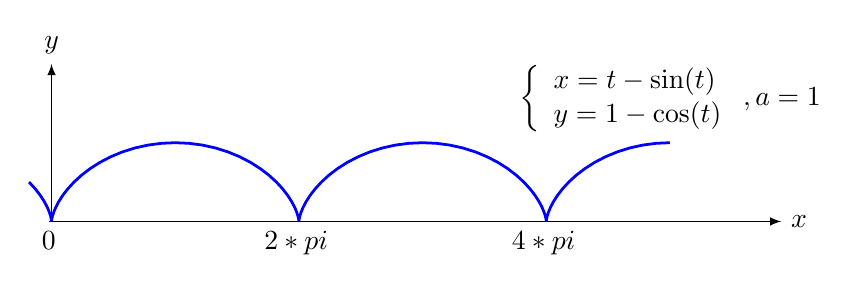
\begin{tikzpicture}[scale=.5]
  	\coordinate (O) at (0,0);
  	\coordinate (A) at (0,4);
  	\def\r{1} % radius
  	\def\c{1.4} % center
  	\coordinate (C) at (\c, \r);
  	
  	\draw[-latex] (O) -- (A) node[anchor=south] {$y$};
  	\draw[-latex] (O) -- (5.9*pi,0) node[anchor=west] {$x$};
	\foreach \pos in {0, 2*pi, 4*pi}
  		\draw[shift={(\pos,0)}] (2pt,0pt) -- (-2pt,0pt) node[below] {$\pos$};
  	\draw[blue,domain=-0.5*pi:5*pi,samples=100, line width=1] 
       	plot ({\x - sin(\x r)},{1 - cos(\x r)}) node[anchor=south, black]{$\left\{\begin{array}{l}
			x = t - \sin(t) \\
			y = 1 - \cos(t) \\	
		\end{array}\right., a=1$};
\end{tikzpicture}

Приклад 2: астроїда $\left\{\begin{array}{l}
	x = a\cos^3 t \\
	y = a\sin^3 t \\	
\end{array}\right., t \in [0, 2\pi]$.

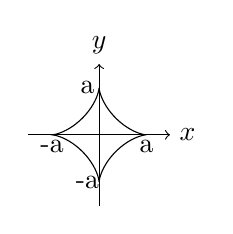
\begin{tikzpicture}[scale=0.6]
	\draw[->] (-1.5,0) -- (1.5,0) node[right] {$x$};
	\draw[->] (0,-1.5) -- (0,1.5) node[above] {$y$};    
    
   	\draw[domain=0:2*pi, samples=100] plot ({(cos(deg(\x)))^3},{(sin(deg(\x)))^3});
   	\draw (1,-0.25) node{a};
    \draw (-0.25,1) node{a};
    \draw (-1,-0.25) node{-a};
    \draw (-0.25,-1) node{-a};
\end{tikzpicture}
\parbox[b]{9cm}{Запишемо рівняння астроїди в неявному вигляді:

$\left(\dfrac{x}{a}\right)^{2/3} + \left(\dfrac{y}{a}\right)^{2/3}
= \cos^2 t + \sin^2 t = 1$

$\Rightarrow x^{2/3} + y^{2/3} = a^{2/3}$.}
	
4) Представлення лінії у полярній системі координат. На площині задана
полярна система координат, якщо задано:
\begin{enumerate}
	\item точка $O$ полюс;
	\item полярна вісь $\rho$ промінь, що виходить з точки $O$.	
\end{enumerate}	


	\begin{wrapfigure}{l}{100px}
		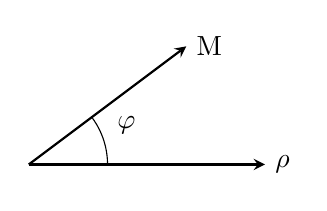
\begin{tikzpicture}[scale=0.5]
			\draw[-stealth, thick] (0,0) -- (6,0) node[anchor=west]{$\rho$};
			\draw[-stealth, thick] (0,0) -- (4,3) node[anchor=west]{M};
				
			\draw[black] (2,0) arc (0:36:2);
			\draw (2,1) node[anchor=west]{$\varphi$};
		\end{tikzpicture}
	\end{wrapfigure}

Тоді положення будь-якої точки $M$ на площині
визначається парою чисел $(\rho, \varphi)$, де полярний радіус
$\rho \geqslant 0$ -- довжина вектора $\overline{OM}$, а полярний кут $\varphi$ це
кут між віссю $\rho$ і $\overline{OM}$, який відраховується проти
годинникової стрілки. Якщо точка $M$ має декартові координати $(x, y)$ і цій парі
чисел відповідає пара $(\rho, \varphi)$, то ця відповідність буде взаємно однозначною, якщо
$\varphi \in [0, 2\pi]$ або $\varphi \in [-\pi, \pi]$. Легко вивести наступні співвідношення (перехід від
полярної системи координат до декартової, і навпаки):

\begin{equation}\label{fromPolarToDekart}
	\left\{\begin{array}{l}
		x = \rho \cos \varphi \\
		y = \rho \sin \varphi \\
	\end{array}\right.
\end{equation}

\begin{equation}\label{fromDekartToPolar}
	\left\{\begin{array}{l}
		\rho = \sqrt{x^2 + y^2} \\
		\left\{\begin{array}{l}
			\cos \varphi = \dfrac{x}{\sqrt{x^2 + y^2}} \\
			\sin \varphi = \dfrac{y}{\sqrt{x^2 + y^2}} \\
		\end{array}\right. \\
	\end{array}\right.
\end{equation}

Приклад: Лемніската Бернуллі $(x^2 + y^2)^2 = a^2(x^2 - y^2), a > 0$.

\parbox{140px}{\begin{tikzpicture}[scale=0.5]
  	\begin{polaraxis}[style=black!10, ticklabel style=black, xticklabel=$\pgfmathprintnumber{\tick}^\circ$]
    	\addplot [thick, black, domain=0:45, samples=50] {2*sqrt(cos(2*x))};
   	 	\addplot [thick, black, domain=-45:0, samples=50] {2*sqrt(cos(2*x))};
   	 	\addplot [thick, black, domain=135:225, samples=100] {2*sqrt(cos(2*x))};
    \end{polaraxis}
\end{tikzpicture}}
\parbox{7.2cm}{З формул \ref{fromDekartToPolar} випливає, що
	$\rho^4 = a^2\rho^2(\cos^2 \varphi - \sin^2 \varphi)$, тобто
	$\rho^2 = a\cos 2 \varphi$ або $\rho = \sqrt{a\cos 2 \varphi}$.
	Область визначення: $\cos 2\varphi \geqslant0$,
	тобто $\varphi \in \left[-\dfrac{\pi}{4}, \dfrac{\pi}{4}\right] \cup \left[\dfrac{3\pi}{4}, \dfrac{5\pi}{4}\right]$.
}

\subsection{Пряма на площині}

Нехай дано пряму $L$.

\begin{definition}[Нормальний вектор прямої]
	\textbf{Нормальний вектор прямої $L$} -- це довільний ненульовий вектор $\overline{n}$, перпендикулярний прямій $L$.
\end{definition}

\begin{figure}[ht]
    \centering
    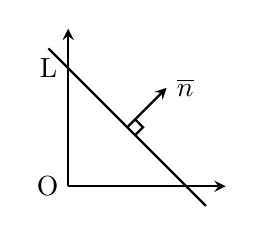
\begin{tikzpicture}[scale=0.5]
        \draw(0,0) node[anchor=east]{O};
        \draw[-stealth, thick] (0,0) -- (4,0);
        \draw[-stealth, thick] (0,0) -- (0,4);
        \draw[thick] (3.5,-0.5) -- (-0.5,3.5)  node[anchor=north]{L};
        \draw[-stealth, thick] (1.5,1.5) -- (2.5,2.5) node[anchor=west]{$\overline{n}$};
        \draw[thick] (1.7,1.7) -- (1.9,1.5) -- (1.7,1.3);
    \end{tikzpicture}
    \caption{Нормальний вектор}
    \label{fig:alg:norm-vector}
\end{figure}

$\overline{n} \perp L$, $\overline{n} \neq \overline{0}$ -- нормальний вектор прямої \ref{fig:alg:norm-vector}.
Зауважимо, що нормальних векторів існує безліч -- з точністю до ненульової константи.


Нехай задано точку $M_0(x_0, y_0)$. Складемо рівняння прямої, що проходить
через точку $M_0(x_0, y_0)$ перпендикулярно до вектора $\overline{n}(A, B)$.

Для довільної точки $M(x, y)$ шуканої прямої вектор $\overline{M_0 M} = (x-x_0, y-y_0)$ є
перпендикулярним вектору $\overline{n}$: $\overline{M_0 M} \perp \overline{n}$, тобто $(\overline{M_0 M}, \overline{n}) = 0$. Отримали:
$A(x-x_0) + B(y-y_0) = 0$ -- рівняння прямої через точку $M_0(x_0, y_0)$ та нормальний вектор $\overline{n}(A, B)$.

Побудуємо загальне рівняння прямої. Розкривши дужки, маємо $Ax + By - (Ax_0 + By_0) = 0$, де $A$ і $B \neq 0$
одночасно. Позначивши $C = -(Ax_0 + By_0)$, отримуємо 

\begin{center}
	$Ax + By + C = 0$ -- \textbf{загальний вигляд прямої}.
\end{center}

\subsection{Неповні рівняння прямої}

\begin{definition}[Повне рівняння прямої]
	Загальне рівняння $Ax + By + C = 0$ -- це \textbf{повне рівняння прямої}, якщо всі його
	коефіцієнти $A \neq 0, B \neq 0, C \neq 0$ (тобто $ABC \neq 0$). Якщо ж хоча б один коефіцієнт
	дорівнює нулю, то це \textbf{неповне рівняння прямої}.
\end{definition}

Розглянемо можливі випадки неповних рівнянь.
\begin{enumerate}
\item $C = 0; L: Ax + By = 0$ -- пряма $L$ проходить через точку $O(0,0)$.
\item $B = 0; L: Ax + C = 0;$ $\overline{n}(A, 0) \perp Oy, L \parallel Oy$.
\item $A = 0; L: By + C = 0;$ $\overline{n}(0, B) \perp Ox, L \parallel Ox$.
\item $B = 0, C = 0; L: Ax = 0$ -- пряма $L$ співпадає з віссю $Oy$.
\item $A = 0, C = 0; L: By = 0$ -- пряма $L$ співпадає з віссю $Ox$.
\end{enumerate}

\subsection{Рівняння прямої у відрізках}

Розглянемо повне рівняння прямої $L: Ax + By + C = 0$, де $ABC \neq 0$.

\begin{center}
	\parbox{4cm}{
		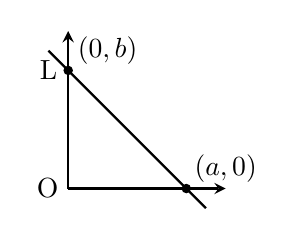
\begin{tikzpicture}[scale=0.5]
			\draw(0,0) node[anchor=east]{O};
			\draw[-stealth, thick] (0,0) -- (4,0);
			\draw[-stealth, thick] (0,0) -- (0,4);
			\draw[thick] (3.5,-0.5) -- (-0.5,3.5)  node[anchor=north]{L};
			\draw (1,3.5) node{$(0,b)$};
			\draw (4,0.5) node{$(a,0)$};
			\filldraw[black] (3,0) circle (3pt);
			\filldraw[black] (0,3) circle (3pt);		
		\end{tikzpicture}
	}
	\parbox{4cm}{
		$$Ax + By = -C;$$
		
		$$\dfrac{x}{-\dfrac{C}{A}} + \dfrac{y}{-\dfrac{C}{B}} = 1.$$
	}
\end{center}

Позначимо $a = -\dfrac{C}{A}, b = -\dfrac{C}{B}$. Тоді маємо рівняння прямої “у відрізках”:

$$\dfrac{x}{a} + \dfrac{y}{b} = 1$$

Геометричний зміст чисел $a$ і $b$: вони дорівнюють величинам відрізків, які
відсікає пряма $L$ на осях $Ox$ та $Oy$ відповідно.

\subsection{Канонічне рівняння}

\begin{definition}[Напрямний вектор]
	\textbf{Напрямний вектор} прямої $L$ -- це довільний ненульовий вектор $q \neq \overline{0}$, що паралельний прямій $L$.
\end{definition}

\parbox{100px}{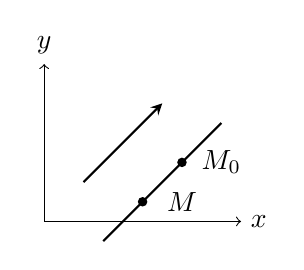
\begin{tikzpicture}[scale=0.5]
	\draw[->] (0,0) -- (5,0) node[right] {$x$};
	\draw[->] (0,0) -- (0,4) node[above] {$y$}; 

	\draw[-stealth, thick] (1,1) -- (3,3);
	\draw[thick] (1.5,-0.5) -- (4.5,2.5);
	\filldraw[black] (2.5,0.5) circle (3pt);			
	\draw (3.5,0.5) node{$M$};
	\filldraw[black] (3.5,1.5) circle (3pt);
	\draw (4.5,1.5) node{$M_0$};
\end{tikzpicture}}
\parbox{8.6cm}{
	Нехай задано точку $M_0(x_0, y_0)$. Складемо рівняння
	прямої, що проходить через точку $M_0(x_0, y_0)$
	паралельно до вектора $\overline{q}(l,m)$ (напрямний вектор).
	Якщо $M(x, y)$ -- це довільна точка шуканої прямої, то
	вектор $\overline{M_0M}$ має координати $(x-x_0, y-y_0)$ і $\overline{M_0M} \parallel \overline{q}$, тобто координати цих
	векторів пропорційні. В результаті маємо \textbf{канонічне рівняння}
}	
	
	\begin{center}
		\fbox{\parbox{4cm}{$$\dfrac{x-x_0}{l} = \dfrac{y-y_0}{m}$$}}
	\end{center}
	 -- рівняння прямої $L$ через точку і напрямний вектор.


\subsection{Параметричне рівняння прямої}

Нехай $\overline{q}(l, m)$ -- це напрямний вектор прямої $L$ і $M_0(x_0, y_0) \in L$. У канонічному
рівнянні даної прямої введемо параметр: $t = \dfrac{x-x_0}{l} = \dfrac{y-y_0}{m}, t \in (-\infty; +\infty)$. Тоді

$$\left\{\begin{array}{l}
	x = lt + x_0 \\
	y = mt + y_0 \\
\end{array}\right.$$

--- \textbf{параметричне рівняння прямої}.

\subsection{Рівняння прямої з кутовим коефіцієнтом}

\noindent\parbox{3.5cm}{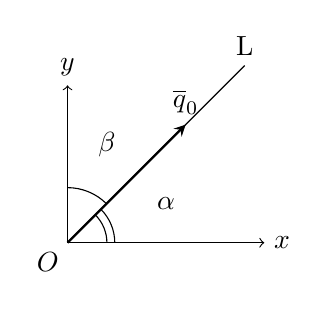
\begin{tikzpicture}[scale=0.5]
	\draw[->] (0,0) -- (5,0) node[right] {$x$};
	\draw[->] (0,0) -- (0,4) node[above] {$y$};
		
	\draw (0,0) -- (4.5,4.5) node[above] {L};			
	\draw[-stealth, thick] (0,0) -- (3,3) node[above] {$\overline{q}_0$};
	\draw (-0.5,-0.5) node{$O$};
	
	\draw[black] (1,0) arc (0:45:1);
	\draw[black] (1.2,0) arc (0:45:1.2);
	\draw (2.5,1) node{$\alpha$};
	
	\draw[black] (0,1.4) arc (90:45:1.4);
	\draw (1,2.5) node{$\beta$};
\end{tikzpicture}}
\parbox{\textwidth - 3.6cm}{
	Розглянемо довільну пряму $L \nparallel Ox$. Нехай $\alpha$ -- це кут нахилу $L$
	до осі $Ox$ (якщо $L \parallel Ox$, то $\alpha = 0$), $\beta$ -- це кут між прямою $L$
	та віссю $Oy$, $\overline{q}(l,m)$ -- це напрямний вектор прямої $L$, $\overline{q}_0$ ---
	це його орт-вектор. Тоді $\overline{q}_0 = (\cos \alpha, \cos \beta) = (\cos \alpha, \sin \alpha)$ (при
	цьому враховано, що $\alpha + \beta = \dfrac{\pi}{2}$). 
}

У цьому випадку канонічне рівняння прямої L буде мати вигляд:

$$\dfrac{x - x_0}{\cos\alpha} = \dfrac{y - y_0}{\sin\alpha}$$

Звідси $y - y_0 = \tg\alpha(x - x_0)$. Якщо позначити $k = \tg\alpha$ -- кутовий коефіцієнт,
то отримаємо рівняння прямої з кутовим коефіцієнтом:
$y - y_0 = k(x - x_0),$
що проходить через точку $M_0(x_0, y_0)$.
Останнє рівняння можна переписати у вигляді:

$$y = kx + b,$$

де $b = y_0 - kx_0$ -- величина відрізка, який відсікає $L$ на осі $Oy$. 

\subsection{Кут між двома прямими}

Кут між двома прямими дорівнює меншому з кутів між їх нормальними або
напрямними векторами. Розглянемо три випадки.

1. Прямі задано загальними рівняннями:

$$\begin{array}{l}
	L_1: A_1x + B_1y + C_1 = 0, \overline{n}_1(A_1,B_1); \\
	L_2: A_2x + B_2y + C_2 = 0, \overline{n}_2(A_2,B_2); \\
\end{array}$$

$$\cos(\widehat{L_1,L_2})
= \cos(\widehat{\overline{n}_1, \overline{n}_2})
= \dfrac{|A_1A_2 + B_1B_2|}{\sqrt{A_1^2+ B_1^2}\sqrt{A_2^2+ B_2^2}}.$$

2. Прямі задано у канонічному вигляді:

$$\begin{array}{l}
	L_1: \dfrac{x - x_1}{l_1} = \dfrac{y - y_1}{m_1}, \overline{q}_1(l_1,m_1); \\
	L_2: \dfrac{x - x_2}{l_2} = \dfrac{y - y_2}{m_2}, \overline{q}_2(l_2,m_2); \\
\end{array}$$

$$\cos(\widehat{L_1,L_2})
= \cos(\widehat{\overline{q}_1, \overline{q}_2})
= \dfrac{|l_1l_2 + m_1m_2|}{\sqrt{l_1^2+ m_1^2}\sqrt{l_2^2+ m_2^2}}.$$

3. Прямі задано рівняннями з кутовими коефіцієнтами: 

$$\begin{array}{l}
	L_1: y = k_1x + b_1, k_1 = \tg\alpha_1; \\
	L_2: y = k_2x + b_2, k_2 = \tg\alpha_2; \\
\end{array}$$

$$\tg(\widehat{L_1,L_2})
= \tg(\alpha_2 - \alpha_1)
= \left|\dfrac{\tg\alpha_2 - \tg\alpha_1}{1+\tg\alpha_1\tg\alpha_2}\right|
= \dfrac{k_2 - k_1}{1+k_1k_2}.$$

\newpage

\parbox{\textwidth - 0.6cm}{\section{Умови перпендикулярності і паралельності прямих}}

Паралельність або перпендикулярність двох прямих рівнозначна
паралельності або перпендикулярності нормальних або напрямних векторів. Тому
відповідно до вигляду рівнянь, якими задані прямі (див. пункти 1 – 3 попереднього
розділу), маємо:

\subsection*{Умови паралельності $L_1 \parallel L_2$:}

\begin{enumerate}
	\item $\overline{n}_1 \parallel \overline{n}_2$ або $\frac{A_1}{A_2} = \frac{B_1}{B_2}$;
	\item $\overline{q}_1 \parallel \overline{q}_2$ або $\frac{l_1}{l_2} = \frac{m_1}{m_2}$;
	\item $k_1 = k_2$.
\end{enumerate}

\subsection*{Умови перпендикулярності $L_1 \perp L_2$:}

\begin{enumerate}
	\item $\overline{n}_1 \perp \overline{n}_2$ або $A_1A_2 + B_1B_2 = 0$;
	\item $\overline{q}_1 \perp \overline{q}_2$ або $l_1l_2 + m_1m_2 = 0$;
	\item $k_1k_2 = -1$.
\end{enumerate}

\subsection{Нормальне рівняння прямої}

% \begin{multicols}{2}
    Нехай $L$ -- пряма, що не проходить через початок координат \ref{fig:alg:norm-equatation-of-the-line}.
    
    \begin{wrapfigure}{l}{0.25\textwidth}
        \centering
        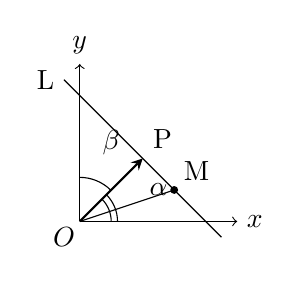
\begin{tikzpicture}[scale=0.4]
            \draw[->] (0,0) -- (5,0) node[right] {$x$};
            \draw[->] (0,0) -- (0,5) node[above] {$y$};
            \draw (-0.5,-0.5) node{$O$};			
                    
            \draw (4.5,-0.5) -- (-0.5,4.5) node[left] {L};			
            \draw[-stealth, thick] (0,0) -- (2,2) node[above right] {P};
                    
            \draw[black] (1,0) arc (0:45:1);
            \draw[black] (1.2,0) arc (0:45:1.2);
            \draw (2.5,1) node{$\alpha$};
            
            \draw[black] (0,1.4) arc (90:45:1.4);
            \draw (1,2.5) node{$\beta$};
                    
            \draw (0,0) -- (3,1) node[above right] {M};
            \filldraw[black] (3,1) circle (3pt);
        \end{tikzpicture}
        % \captionof{figure}{Нормальне рівняння прямої}
        \label{fig:alg:norm-equatation-of-the-line}
    \end{wrapfigure}
 
    
    Проведемо нормальний вектор $\overline{n}$ так:
    \begin{enumerate}
        \item його початок -- в точці $(0,0)$, а кінець лежить на прямій;
        \item $|\overline{n}| = p>0$ (такий вектор єдиний!).
        \item Кут $\alpha$ -- це кут між віссю $OX$ і $\overline{n}$, який відраховується проти годинникової стрілки.
    \end{enumerate}
    
    Нехай точка $M(x,y) \in L$. Тоді $\overline{OM}(x,y)$ -- це її радіус-вектор, $\overline{n}_0$ -- це орт вектор
    нормального вектора $\overline{n}$: $\overline{n}_0 = (\cos\alpha,\cos\beta) = (\cos\alpha,\sin\alpha)$.
    
    При цьому враховано, що $\alpha + \beta = \dfrac{\pi}{2}$.
    
    Мають місце наступні співвідношення:

    \begin{equation*}
        \begin{split}
            p
            &= |OP|\\
            &= \text{пр}_{\overline{n}}\overline{OM} = \text{пр}_{\overline{n}_0}\overline{OM}\\
            &= |OM|\cos(\widehat{\overline{n}_0,OM})\\
            &= |OM|\dfrac{(\overline{n}_0,\overline{OM})}{|\overline{n}_0||\overline{OM}|}\\
            &= \dfrac{(\overline{n}_0,\overline{OM})}{|\overline{n}_0|}\\
            &= x\cos\alpha + y\sin\alpha.\\
        \end{split}
    \end{equation*}
    
    Отримали рівняння
    $x\cos\alpha + y\sin\alpha = 0$,	
    -- це \textbf{нормальне рівняння прямої $L$}, де $p$ -- це відстань від початку
    координат до прямої $L$.
% \end{multicols}

\section{Зведення загального рівняння прямої до нормального вигляду}

Розглянемо загальне рівняння прямої $L: Ax + By + C= 0$, та нормальне
рівняння цієї прямої: $x\cos\alpha + y\sin\alpha - p = 0$.

Для того, щоб рівняння були рівносильними, достатньо, щоб їх коефіцієнти
були пропорційними: $\dfrac{\cos\alpha}{A} = \dfrac{\sin\alpha}{b} = \dfrac{-p}{C} = \mu$, де $\mu$ -- це
\textbf{нормуючий множник}. Тоді $\cos\alpha = \mu A, \sin\alpha = \mu B, -p = \mu C$. Звідси визначимо $\mu$:

$$\mu^2(A^2 + B^2) = \cos^2\alpha + \sin^2\alpha = 1 \Rightarrow \mu = \dfrac{1}{\pm\sqrt{A^2 + B^2}}.$$

Знак $\mu$ визначається рівністю $\mu C = -p$. Оскільки $p \geq 0$, то знак нормуючого
множника $\mu$ є протилежним до знаку $C$. Отже, \textbf{нормальне рівняння прямої} $L$ буде
мати вигляд

$\mu(Ax+By+C) = 0$, де $\mu = \dfrac{-\text{sign} C}{\sqrt{A^2 + B^2}}$ -- нормуючий множник.

\begin{example}
	Звести рівняння прямої $L : 3x-4y+25 = 0$ до нормального виду.
\end{example}
\begin{solution}
	Знайдемо нормуючий множник:

	$\mu = -\dfrac{1}{\sqrt{3^2 + (-4)^2}}$.
	Тоді $-\frac{3}{5} x + \frac{4}{5} y - 5 = 0$ -- нормальне рівняння $L$, де
	$\cos\alpha = -\frac{3}{5}, \sin\alpha = \frac{4}{5}, p = 5$ -- довжина перпендикуляра,
	опущеного з точки O на цю пряму. 
\end{solution}

\subsection{Відхилення і відстань від точки до прямої}
\begin{wrapfigure}{l}{0.25\textwidth}
    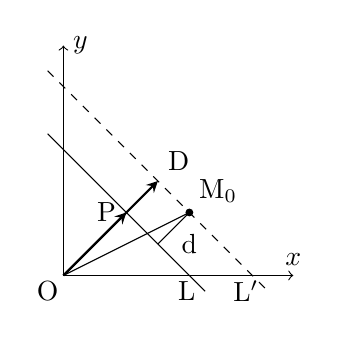
\begin{tikzpicture}[scale=0.4]
        \draw[->] (0,0) -- (7.3,0) node[above] {$x$};
        \draw[->] (0,0) -- (0,7.3) node[right] {$y$};
        \draw (-0.5,-0.5) node{O};
        %\draw[gray, dashed] (0,0) grid (7.3,7.3);
                    
        \draw (-0.5,4.5) -- (4.5,-0.5) node[left] {L};
        \draw[dashed] (-0.5,6.5) -- (6.5,-0.5) node[left] {L$'$};
        \draw[-stealth, thick] (0,0) -- (2,2) node[left] {P};
        \draw[-stealth, thick] (0,0) -- (3,3) node[above right] {D};
            
        \draw (0,0) -- (4,2) node[above right] {M$_0$};
        \draw (3,1) -- (4,2);
        \draw (4,1) node{d};
        \filldraw[black] (4,2) circle (3pt);
    \end{tikzpicture}
    \caption{Відхилення і відстань від точки до прямої}
    \label{fig:alg:deviation-and-distance-from-the-point-to-the-line}
\end{wrapfigure}

Нехай задано пряму $L$ , точку $M_0(x_0,y_0)\not\in L$,
відстань від якої до даної прямої дорівнює
$d = \rho(M_0, L) > 0$ \ref{fig:alg:deviation-and-distance-from-the-point-to-the-line}. Точка $O(0,0)$ -- це
початок координат.

Нехай пряма $L$ задається нормальним
рівнянням: $x\cos\alpha + y\sin\alpha - p = 0$.


\begin{definition}[Відхилення точки від прямої]
	\textbf{Відхилення} точки $M_0$ від прямої $L$ -- це число

	$$\delta_{M_0,L}\left\{\begin{array}{l}
		d\text{, якщо точки } M_0 \text{ і } O \text{ лежать по різні сторони прямої;} \\
		-d\text{, якщо точки } M_0 \text{ і } O \text{ лежать по один бік від прямої.} \\
	\end{array}\right.$$
\end{definition}


Обчислимо відхилення $\delta_{M_0,L}$. Для цього через точку $M_0$ проведемо пряму $L'$,
паралельну $L$. Побудуємо $OD \perp L'$. Тоді рівняння $L'$ має вигляд:

$$x\cos\alpha + y\sin\alpha - p - \delta_{M_0,L} = 0.$$

Але координати точки $M_0(x_0,y_0)$ задовольняють це рівняння, тому
$x_0\cos\alpha + y_0\sin\alpha - p - \delta_{M_0,L} = 0$.

Таким чином, відхилення точки $M_0$ від прямої $L$ обчислюється за формулою:
$$\delta_{M_0,L} = x_0\cos\alpha + y_0\sin\alpha - p$$

(для того, щоб знайти відхилення точки $M_0$ від прямої $L$ , потрібно підставити
координати цієї точки в нормальне рівняння даної прямої).

Відстань від точки $M_0(x_0,y_0) \not\in L$ до прямої $L$ обчислюється таким чином:
$$d = |\delta_{M_0,L}| = |x_0\cos\alpha + y_0\sin\alpha - p|$$.

Якщо ж пряма задається загальним рівнянням, то 
$$d = \dfrac{|Ax_0 + By_0 + C|}{\sqrt{A^2 + B^2}}$$.

\begin{problem}[З’ясувати, в якому куті (гострому чи тупому), утвореному при перетині двох прямих, знаходиться задана точка]
	З’ясувати, в якому куті (гострому чи тупому), утвореному при перетині
	прямих $L_1$ та $L_2$, знаходиться точка $M_0(-2,2)$, якщо $L_1: 2x - y + 2 = 0$, 
	$L_2: 4x + y - 4 = 0$. В яких кутах (суміжних чи вертикальних) знаходяться точка
	$M_0$ та початок координат $O(0,0)$? 
\end{problem}
\begin{solution}
	З’ясуємо, який кут (гострий чи тупий) утворюють орти
	нормальних векторів прямих $L_1$ та $L_2$. Спочатку запишемо рівняння даних прямих
	у нормальному вигляді:
	
	$$\begin{array}{ll}
		L_1: -\dfrac{1}{\sqrt{5}}(2x - y + 2) = 0; & \overline{n}_1^0 = -\dfrac{1}{\sqrt{5}}(2,-1) = \dfrac{1}{\sqrt{5}}(-2,1);  \\
		L_1: \dfrac{1}{\sqrt{17}}(4x + y - 4) = 0; & \overline{n}_2^0 = \dfrac{1}{\sqrt{17}}(4,1);  \\
	\end{array}$$
	
	\noindent\parbox{4.5cm}{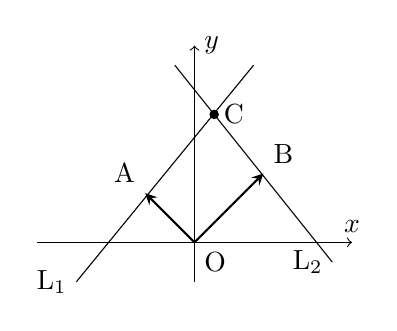
\begin{tikzpicture}[scale=0.5]
		\draw[->] (-4,0) -- (4,0) node[above] {$x$};
		\draw[->] (0,-1) -- (0,5) node[right] {$y$};
		\draw (0,0) node[below right]{O};
			
		\draw (1.5,4.5) -- (-3,-1) node[left] {L$_1$};
		\draw (-0.5,4.5) -- (3.5,-0.5) node[left] {L$_2$};
		\draw[-stealth, thick] (0,0) -- (-1.25,1.25) node[above left] {A};
		\draw[-stealth, thick] (0,0) -- (1.75,1.75) node[above right] {B};
		\filldraw (0.5,3.25) circle (3pt) node[right]{C};
	\end{tikzpicture}}
	\parbox{\textwidth - 4.6cm}{
		Оскільки скалярний добуток

		$$(\overline{n}_1^0,\overline{n}_2^0) = \frac{1}{\sqrt{5}\sqrt{17}}(-8+1) < 0,$$
		
		то кут $AOB$
		між векторами $\overline{n}_1^0$ та $\overline{n}_2^0$ -- тупий. У
		чотирикутнику $AOBC$ $\angle A$ та $\angle B$ -- прямі,
		$\angle AOB$ -- тупий, тому $\angle ACB$ -- гострий.
		
		Отже, початок координат $O(0,0)$ знаходиться в гострому куті, утвореному при
		перетині прямих $L_1$ та $L_2$.
	}
	
	Знайдемо відхилення точки $M_0(-2,2)$ від даних прямих.
	
	\noindent\parbox{2.4cm}{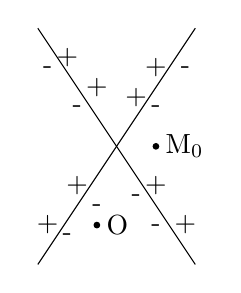
\begin{tikzpicture}[scale=0.5]
		\draw (-2,3) -- (2,-3);
		\draw (-2,-3) -- (2,3);
				
		\draw (1,1) node{-};
		\draw (1.75,2) node{-};
		\draw (0.5,1.25) node{+};
		\draw (1,2) node{+};
				
		\draw (-0.5,1.5) node{+};
		\draw (-1.25,2.25) node{+};
		\draw (-1,1) node{-};
		\draw (-1.75,2) node{-};
				
		\draw (1,-1) node{+};
		\draw (1.75,-2) node{+};
		\draw (0.5,-1.25) node{-};
		\draw (1,-2) node{-};
				
		\draw (-0.5,-1.5) node{-};
		\draw (-1.25,-2.25) node{-};
		\draw (-1,-1) node{+};
		\draw (-1.75,-2) node{+};
				
		\filldraw (1,0) circle (2pt) node[right]{M$_0$};
		\filldraw (-0.5,-2) circle (2pt) node[right]{O};
	\end{tikzpicture}}
	\parbox{\textwidth - 2.5cm}{
		$\delta_{M_0,L_1} = -\dfrac{1}{\sqrt{5}}(-4 -2 +2) = \dfrac{4}{\sqrt{5}} > 0;$
	
		$\delta_{M_0,L_2} = \dfrac{1}{\sqrt{17}}(-8 +2 -4) = -\dfrac{10}{\sqrt{17}} < 0;$
	
		Дві прямі, що перетинаються, ділять площину на
		чотири області. На рисунку зображено знаки відхилень
		точок, які лежать в кожній з чотирьох областей, при умові, що початок координат
		$O(0,0)$ знаходиться в гострому куті.
	}
	
	Враховуючи знаки відхилень точки $M_0$ від даних прямих, робимо висновок,
	що точка $M_0$ лежить в тупому куті, утвореному при перетині прямих $L_1$ та $L_2$.
	
	Точки $O(0,0)$ та $M_0$ лежать в суміжних кутах. 
\end{solution}

\subsection{Рівняння пучка (низки) прямих}

\begin{definition}[Пучок прямих (низка прямих)]
	\textbf{Пучок прямих (низка прямих)} на площині з центром у даній точці -- це  
	сукупність прямих, що проходить через цю точку.
\end{definition}

Якщо задана точка $M_0(x_0,y_0)$, то рівняння $A(x - x_0) + B(y - y_0) = 0$ при
змінних коефіцієнтах $A$ і $B$, а також рівняння $y-y_0 = k(x-x_0)$ при змінному $k$
є рівняннями пучка (низки) прямих з центром у точці $M_0$.

Пучок прямих можна задати довільними двома прямими, які перетинаються у
точці $M_0$:

$$\begin{array}{l}
	L_1: A_1x + B_1y + C_1 = 0,\\
	L_2: A_2x + B_2y + C_2 = 0.\\
\end{array}$$

Рівняння пучка прямих із центром у точці $M_0$ можна записати, не визначаючи
координат $M_0$:

$$A_1x + B_1y + C_1 + \lambda(A_2x + B_2y + C_2) = 0.$$

Щоб із пучка прямих виділити певну пряму, потрібно задати додаткову умову
для знаходження параметра $\lambda$, що відповідає шуканій прямій. 

\section{Криві другого порядку}

Загальне рівняння кривої другого порядку має такий вигляд:

$$Ax^2 + By^2 + Cxy + Dx + Ey + F = 0$$

При різних значеннях коефіцієнтів можемо отримати вироджені випадки:
прямі, точки, криві лінії. Ми ж будемо розглядати невироджені випадки кривих
другого порядку – еліпс, гіперболу, параболу. 

\subsection{Канонічне рівняння еліпса}

\begin{definition}[Еліпс]
	Еліпсом називається геометричне місце точок площини таких, що сума
	відстаней від кожної з яких до двох фіксованих точок (фокусів) є величина стала. 
\end{definition}

\noindent\parbox{4cm}{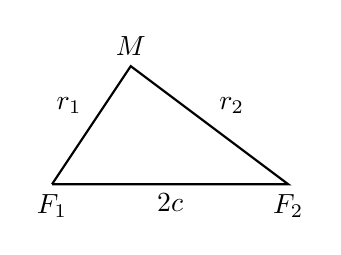
\begin{tikzpicture}[scale=0.5]
	\draw[thick] (-3,0)node[below]{$F_1$} -- (-1,3)node[above]{$M$} -- (3,0)node[below]{$F_2$} -- (-3,0);
	\draw (-2,2)node[left]{$r_1$};
	\draw (1,2)node[right]{$r_2$};
	\draw (0,0)node[below]{$2c$};
\end{tikzpicture}}
\parbox{\textwidth - 4.1cm}{
	Отже, маємо два фокуси $F_1$ і $F_2$, відстань між ними $|F_1F_2| = 2c$. Нехай $M$ – довільна точка
	еліпса. Відрізки $r_1 = |F_1M|$ та $r_2 = |F_2M|$
	називаються фокальними радіусами точки $M$.

	За означенням еліпса: $r_1 + r_2 = 2a$.
}

З трикутника $F_1MF_2$ маємо: $|F_1M| + |F_2M| > |F_1F_2|$, тобто $2a > 2c$, або $a>c$.

\noindent\parbox{6cm}{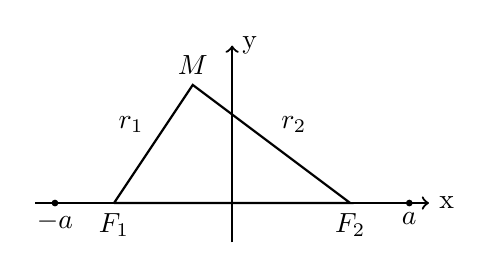
\begin{tikzpicture}[scale=0.5]
	\draw[->, thick] (-5,0) -- (5,0)node[right]{x};
	\draw[->, thick] (0,-1) -- (0,4)node[right]{y};
  	
  	%\draw (-5,-2) grid (5,5);
	\draw[thick] (-3,0)node[below]{$F_1$} -- (-1,3)node[above]{$M$} -- (3,0)node[below]{$F_2$} -- (-3,0);
	\draw (-2,2)node[left]{$r_1$};
	\draw (1,2)node[right]{$r_2$};
	
	\filldraw[black] (-4.5,0) circle(2pt) node[below]{$-a$};
	\filldraw[black] (4.5,0) circle(2pt) node[below]{$a$};
\end{tikzpicture}}
\parbox{\textwidth - 6.1cm}{
	Побудуємо декартову систему
	координат. Нехай вісь $OX$
	пройде через фокуси $F_1$ і $F_2$ ,а
	вісь $OY$ -- через середину
	відрізка $F_1F_2$ . Відповідно до
	вибраної системи координат
	фокуси будуть мати такі
	координати: $F_1(-c,0), F_2(c,0)$. 
}

Оскільки точка $M$ -- це довільна точка еліпса, то вона має координати $(x,y)$. Тоді

$$r_1 = |F_1M| = \sqrt{(x+c)^2+y^2}, r_2 = |F_2M| = \sqrt{(x-c)^2+y^2}.$$

Враховуючи умову $r_1 + r_2 = 2a$, маємо рівняння еліпса:

$$\sqrt{(x+c)^2+y^2} + \sqrt{(x-c)^2+y^2} = 2a.$$

Піднесемо до квадрату обидві частини рівняння:

$$(x+c)^2+y^2 + (x-c)^2+y^2 + 2\sqrt{((x+c)^2+y^2)((x-c)^2+y^2)} = 4a^2.$$

Перегрупувавши доданки, маємо:

$$x^2 + 2xc + c^2 + y^2 + x^2 - 2xc + c^2 + y^2 - 4a^2 = $$

$$= -2\sqrt{((x^2 + y^2 + c^2) + 2xc)((x^2 + y^2 + c^2) - 2xc)}.$$

Виконавши елементарні перетворення, отримаємо: 

$$\sqrt{(x^2 + y^2 + c^2)^2 - 4x^2c^2} = 2a^2 - (x^2 + y^2 + c^2).$$

Знову піднесемо до квадрату та отримаємо:

$$(x^2 + y^2 + c^2)^2 - 4x^2c^2 = (x^2 + y^2 + c^2)^2 + 4a^4 - 4a^2(x^2 + y^2 + c^2).$$

\begin{center}
	або
\end{center}	
	
$$x^2(a^2 - c^2) + y^2a^2 = a^4 - a^2c^2.$$

Позначивши $b^2 = a^2 - c^2$ (оскільки $a>c$), маємо: $x^2b^2 + y^2a^2 = a^2b^2$.
Поділивши обидві частини цієї рівності на $a^2b^2$, отримуємо \textbf{канонічне рівняння
еліпса:}

\begin{wrapfigure}{l}{4.5cm}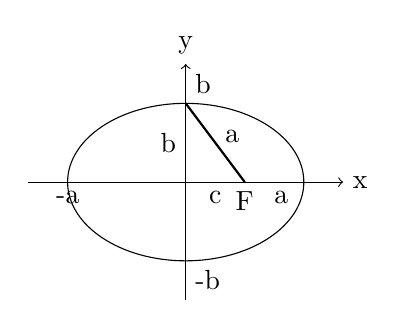
\begin{tikzpicture}[scale=0.5]
	\draw[->] (-4,0) -- (4,0)node[right]{x};
	\draw[->] (0,-3) -- (0,3)node[above]{y};
  	
	\draw (0,0) ellipse (3cm and 2cm);
	\draw[thick] (0,2) -- (1.5,0);
	
	\draw (-3,0)node[below]{-a};
	\draw (0,2)node[above right]{b};
	\draw (1.5,0)node[below]{F};
	\draw (0,-2)node[below right]{-b};
	\draw (2,0)node[below right]{a};
	\draw (0.75,0)node[below]{c};
	\draw (0,1)node[left]{b};
	\draw (0.75,0.75)node[above right]{a};
\end{tikzpicture}\end{wrapfigure}

$$\dfrac{x^2}{a^2} + \dfrac{y^2}{b^2} = 1.$$

Дослідимо форму еліпса. З отриманого рівняння
випливає, що для всіх точок еліпса
$x^2 \leqslant a^2$, $y^2 \leqslant b^2$, або $|x| \leqslant a$, $|y| \leqslant b$, тобто це
означає, що всі точки еліпса знаходяться всередині
прямокутника, сторони якого паралельні осям координат і мають довжини $2a$ та
$2b$, де $a$ -- це \textbf{велика піввісь}, $b$ -- \textbf{мала піввісь} ($a>b$). Кожна точка
$(a,0)$, $(-a,0)$, $(0,b)$, $(0,-b)$, в якій еліпс перетинає осі координат, -- це
\textbf{полюс еліпса (або вершина еліпса)}. Якщо довільні значення $(x,y)$, задовольняють
канонічне рівняння еліпса, то очевидно, що значення $(-x,y)$, $(x,-y)$, $(-x,-y)$ теж будуть
задовольняти рівняння еліпса. Це означає, що координатні осі, кожна з них -- це \textbf{вісь
симетрії}, а точка $O(0,0)$ -- \textbf{центр симетрії еліпса}. 

\subsection{Канонічне рівняння гіперболи}

\begin{definition}[Гіпербола]
	\textbf{Гіпербола} -- це геометричне місце точок площини, для яких
	модуль різниці відстаней від двох фіксованих точок (фокусів) є сталою величиною.
\end{definition}

Нехай $F_1$ і $F_2$ -- фокуси, відстань між якими $|F_1F_2| = 2c$, $M$ -- довільна точка
гіперболи, $r_1$ та $r_2$ -- це фокальні радіуси точки $M$.
Згідно з означенням гіперболи $|r_1 - r_2| = 2a$.
З трикутника $F_1MF_2$ маємо: $2a < 2c$, тобто $a < c$.
Побудову декартової системи координат і подальші
викладки здійснюємо так само, як і при виведенні рівняння еліпса:

$$F_1(-c,0), F_2(c,0), M(x,y),$$

$$r_1 = \sqrt{(x + c)^2 + y^2}, r_2 = \sqrt{(x - c)^2 + y^2},$$

$$|r_1 - r_2| = 2a,$$

$$|\sqrt{(x + c)^2 + y^2} - \sqrt{(x - c)^2 + y^2}| - 2a,$$

$$(x^2 + y^2 + c^2) + 2xc + (x^2 + y^2 + c^2) - 2xc -$$

$$-2\sqrt{((x^2+y^2+c^2)+2xc)((x^2+y^2+c^2)-2xc)} =4a^2,$$

$$(x^2+y^2+c^2) - 2a^2 = \sqrt{v^2 - 4x^2c^2},$$

$$(x^2+y^2+c^2) - 4a^2(x^2+y^2+c^2) + 4a^4 = (x^2+y^2+c^2)^2 - 4x^2c^2,$$

$$x^2c^2 - x^2a^2 - y^2a^2 = a^2c^2 - a^4,$$

$$x^2(c^2 - a^2) - y^2a^2 = a^2(c^2 - a^2).$$

Позначимо $B^2 C^2 - A^2$ (враховуючи, що $c>a$). Тоді

$$x^2b^2 - y^2a^2 = a^2b^2.$$

В результаті перетворень отримали \textbf{канонічне рівняння гіперболи}:

$$\dfrac{x^2}{a^2} - \dfrac{y^2}{b^2} = 1$$

З отриманого рівняння випливає, що

$$x^2 = a^2\left(1 + \dfrac{y^2}{b^2}\right) \Rightarrow x \leqslant -a \text{ або } x \geqslant a.$$

Аналогічно,

$$y^2 = b^2\left(\dfrac{x^2}{a^2} - 1\right) \Rightarrow y = \pm\dfrac{b}{a}\sqrt{x^2 - a^2} \Rightarrow y \in (-\infty; +\infty).$$

\begin{wrapfigure}{l}{4.5cm}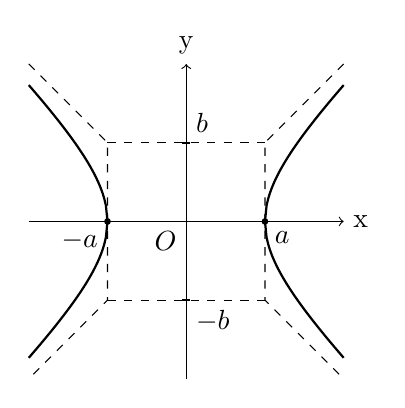
\begin{tikzpicture}[scale=0.5]
	\draw[->] (-4,0) -- (4,0)node[right]{x};
	\draw[->] (0,-4) -- (0,4)node[above]{y};
	
	\def\a{2};
	\def\b{2};
	
	\draw[domain=\a:4, samples=50, thick] plot (\x,{(\b/\a)*sqrt(\x^2 - \a^2)});
	\draw[domain=\a:4, samples=50, thick] plot (\x,{-(\b/\a)*sqrt(\x^2 - \a^2)});
	\draw[domain=\a:4, samples=50, thick] plot ({-\x},{(\b/\a)*sqrt(\x^2 - \a^2)});
	\draw[domain=\a:4, samples=50, thick] plot ({-\x},{-(\b/\a)*sqrt(\x^2 - \a^2)});
	
	\draw[dashed] (-4,4) -- (-2,2) -- (-2,-2) -- (-4,-4);
	\draw[dashed] (4,4) -- (2,2) -- (2,-2) -- (4,-4);
	\draw[dashed] (-2,2) -- (2,2);
	\draw[dashed] (-2,-2) -- (2,-2);
	
	\filldraw[black] (2,0) circle(2pt) node[below right]{$a$};
	\filldraw[black] (-2,0) circle(2pt) node[below left]{$-a$};
	\draw[thick] (-0.1,2) -- (0.1,2);
	\draw[thick] (-0.1,-2) -- (0.1,-2);
	\draw (0,2)node[above right]{$b$};
	\draw (0,-2)node[below right]{$-b$};
	\draw (0,0)node[below left]{$O$};
\end{tikzpicture}\end{wrapfigure}

Тобто гіпербола є необмеженою
кривою, яка складається з двох гілок,
які є симетричними відносно осі $OY$ і
лежать праворуч від прямої $x = a$ та
ліворуч від прямої $x = -a$.

Координатні осі -- це осі симетрії, точка
$O$ -- центр симетрії гіперболи.
Асимптотами гіперболи є прямі
$y = \pm\dfrac{b}{a}x$.

Доведемо це для гілки гіперболи, що лежить у першій чверті: 

$$\dfrac{y^2}{b^2} = \dfrac{x^2}{a^2} - 1 \Rightarrow y = \dfrac{b}{a}\sqrt{x^2 - a^2},$$

тобто

$$\lim\limits_{x \rightarrow +\infty}\dfrac{\dfrac{b}{a}\sqrt{x^2-a^2}}{\dfrac{b}{a}x}
= \lim\limits_{x \rightarrow +\infty}\sqrt{1 - \dfrac{a^2}{x^2}} = 1.$$

Це означає, що чисельник наближається до знаменника, тобто крива при
$x \rightarrow +\infty$ наближається до своєї асимптоти. Для трьох інших чвертей викладки
аналогічні. 

\subsection{Канонічне рівняння параболи}

\begin{definition}[Парабола]
	\textbf{Парабола} -- це геометричне місце точок площини, кожна з яких
	однаково віддалена від фіксованої точки (фокуса) і від даної прямої (директриси).
\end{definition}

Відстань від фокуса $F$ до директриси $D$ позначимо $p$. Нехай $M$ -- довільна
точка параболи. Тоді $r = |FM|$ -- фокальний радіус точки $M$.

\noindent\parbox{4.5cm}{
	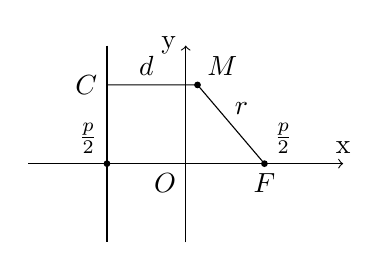
\begin{tikzpicture}[scale=0.5]
		\draw[->] (-4,0) -- (4,0)node[above]{x};
		\draw[->] (0,-2) -- (0,3)node[left]{y};

		\draw (0,0)node[below left]{$O$};
		\draw (-2,3) -- (-2,-2);
		\draw (-2,2)node[left]{$C$} -- (0.3,2)node[above right]{$M$} -- (2,0)node[below]{$F$};
		\filldraw[black] (0.3,2) circle(2pt);	
		\filldraw[black] (-2,0) circle(2pt) node[above left]{$\frac{p}{2}$};
		\filldraw[black] (2,0) circle(2pt) node[above right]{$\frac{p}{2}$};
		\draw (-1,2) node[above]{$d$};
		\draw (1,1) node[above right]{$r$};
	\end{tikzpicture}
}\parbox{\textwidth - 4.5cm}{
	Декартову систему координат будуємо
	таким чином: вісь $OX$ проходить через
	фокус $F$ перпендикулярно директрисі $D$, а
	вісь $OY$ -- через середину відстані від $F$ до
	$D$. Тоді $M(x,y)$, $F(\frac{p}{2}, 0)$, $d = \rho(M,D) = |MC| = x + \frac{p}{2}$,
	а фокальний радіус $r = |FM| = \sqrt{(x-\frac{p}{2})^2 + y^2}.$
}

За означенням $d = r$, тобто

$$x + \frac{p}{2} = \sqrt{(x-\frac{p}{2})^2 + y^2} \Rightarrow x ^2 + xp + \frac{p^2}{4} = x^2 - xp + \frac{p^2}{4} + y^2.$$

\noindent\parbox{5cm}{
	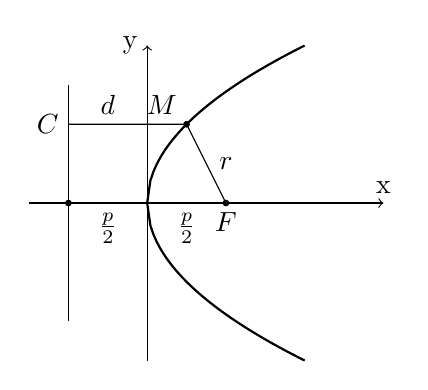
\begin{tikzpicture}[scale=0.5]
		\draw[->] (-3,0) -- (6,0)node[above]{x};
		\draw[->] (0,-4) -- (0,4)node[left]{y};
		
		\draw (-2, 3) -- (-2,-3);	
		\filldraw[black] (-2,0) circle(2pt);
		\filldraw[black] (2,0) circle(2pt);
		\draw (-1,0)node[below]{$\frac{p}{2}$};
		\draw (1,0)node[below]{$\frac{p}{2}$};
		\draw (-2,2)node[left]{$C$} -- (1,2)node[above left]{$M$} -- (2,0)node[below]{$F$};
		\filldraw[black] (1,2) circle(2pt);
		\draw(-1,2)node[above]{$d$};
		\draw(2,1)node{$r$};
			
		\draw[domain=0:4, samples=50, thick] plot ({\x},{sqrt(4*\x)});
		\draw[domain=0:4, samples=50, thick] plot ({\x},{-sqrt(4*\x)});
	\end{tikzpicture}
}\parbox{\textwidth - 5cm}{
	Отримали \textbf{канонічне рівняння
	параболи}: $y =2px$, де $p$ ---
	параметр, $p > 0$.
	Очевидно, що $x \geqslant 0 $. Отже,
	парабола розташована праворуч від
	осі $OY$. З отриманого рівняння
	випливає, що для довільного значення
	$x$ існує два протилежні значення $y$:
	$y = \pm\sqrt{2px}$, а це означає, що
	парабола симетрична відносно осі $OX$ (осі параболи). Парабола проходить через
	точку $O(0,0)$, яка називається її вершиною. Якщо $x \rightarrow +\infty$, то
	$y \rightarrow +\infty$, що означає, що вітки параболи простягаються в нескінченність. 
}

\subsection{Ексцентриситет і директриси еліпса і гіперболи}

\begin{definition}[Ексцентриситет]
	Величина $\varepsilon = \dfrac{c}{a}$ -- це \textbf{ексцентриситет еліпса} і \textbf{ексцентриситет гіперболи}.
\end{definition}

Для еліпса $\varepsilon = \dfrac{c}{a} = \dfrac{\sqrt{a^2 - b^2}}{a} = \sqrt{1-\dfrac{b^2}{a^2}}$,
тому $\varepsilon \in [0;1)$. Якщо $\varepsilon = 0$, то це
означає, що $a=b$ і $c=0$, тобто фокуси еліпса збігаються, і еліпс перетворюється
в коло. Ексцентриситет характеризує форму даної кривої. Чим більше $\varepsilon$, тим
більше еліпс “сплющується” по осі OY.

Для гіперболи $\varepsilon = \dfrac{c}{a} = \dfrac{\sqrt{a^2 + b^2}}{a} = \sqrt{1+\dfrac{b^2}{a^2}}$,
тобто $\varepsilon \in (1;+\infty)$. Із зростанням $\varepsilon$ гілки гіперболи “розпрямлюються”.

\begin{definition}[Директриса]
	\textbf{Директриса еліпса (директриса гіперболи)} -- це дві прямі, які
	перпендикулярні фокальній осі (тобто до осі, на якій розміщені фокуси) і
	знаходяться на відстані $\dfrac{a}{\varepsilon}$ від центра кривої.
\end{definition}

У вибраній системі координат директриси еліпса та гіперболи паралельні осі
$OY$ і не перетинають самі криві. Отже, рівняння директрис $D_1$ і $D_2$ для цих двох
кривих мають вигляд: $x = \pm\dfrac{a}{\varepsilon}$ або $x = \pm\dfrac{a^2}{c}$.

Для еліпса $a > c \Rightarrow \dfrac{a}{c} > 1$, тому $\dfrac{a^2}{c} = \dfrac{aa}{c} > a$
(враховано, що $\varepsilon = \dfrac{c}{a}$ і $0 \leqslant \varepsilon < 1$). Це
означає, що директриси еліпса лежать поза його межами.

Аналогічно для гіперболи $a < c \Rightarrow \dfrac{a}{c} < 1$ і $\dfrac{a^2}{c} = \dfrac{aa}{c} < a$,
тобто директриси гіперболи знаходяться між її гілками.

Для доведення теореми про зв’язок між поняттями ексцентриситет і
директриса роз\-в’я\-же\-мо наступну задачу.

\begin{problem}[Формула фокального радіуса довільної точки еліпса]
	Довести, що фокальні радіуси $r_1$ і $r_2$ довільної точки еліпса мають
	вигляд: $r_1 = a + \varepsilon x$, $r_2 = a - \varepsilon x$. 
\end{problem}
\begin{solution}
	Нехай точка $M(x,y)$ -- довільна точка еліпса. Тоді її координати
	задовольняють канонічне рівняння еліпса $\dfrac{x^2}{a^2} + \dfrac{y^2}{b^2} = 1$. Звідси $y^2 = b^2(1-\dfrac{x^2}{a^2})$
	або $y^2 = \dfrac{b^2}{a^2}(a^2-x^2)$. Знайдемо фокальний радіус $r_1$:

	$$r_1 = |F_1M| = \sqrt{(x+c)^2 + y^2} = \sqrt{x^2 + 2xc + c^2 + \dfrac{b^2}{a^2}(a^2-x^2)} =$$

	$$= \sqrt{x^2 + 2xc + c^2 + \dfrac{a^2-c^2}{a^2}(a^2-x^2)} = \sqrt{x^2 + 2xc + c^2 + (1-\dfrac{c^2}{a^2})(a^2-x^2)} =$$

	$$\sqrt{a^2 + 2xc + \dfrac{c^2}{a^2}x^2} = \sqrt{(a + \dfrac{c}{a}x)^2} = |a + \dfrac{c}{a}x| = |a + \varepsilon x|.$$

	Знайдемо знак виразу $a + \varepsilon x$. Оскільки $\dfrac{c}{a} < 1$ і $|x| \leqslant a$, то $|\dfrac{c}{a}x| < a$.
	Тому $a + \dfrac{c}{a}x > 0$, тобто $a + \varepsilon x > 0$ і $r_1 = a + \varepsilon x$, що і треба було довести. Фокальний
	радіус $r_2$ знаходиться аналогічно.
\end{solution}

Зауважимо, що для гіперболи аналогічними міркуваннями можна отримати: $r_1 = \varepsilon x + a$, $r_2 = \varepsilon x - a$.

\begin{theorem}
	Якщо $M(x,y)$ -- довільна точка еліпса чи гіперболи, $r_1$ і $r_2$ -- її
	фокальні радіуси, $\rho(M,D_1)$ і $\rho(M,D_2)$ -- відстані від точки $M$ до відповідної
	директриси, то має місце співвідношення:
	
	$$\dfrac{r_1}{\rho(M,D_1)} = \dfrac{r_2}{\rho(M,D_2)} = \varepsilon$$
\end{theorem}
\begin{proof}(проведемо для еліпса):
	
	$$\dfrac{r_1}{\rho(M,D_1)} = \dfrac{r_1}{d_1} = \dfrac{a + \varepsilon x}{x + \dfrac{a}{\varepsilon}}
	= \varepsilon\dfrac{a + \varepsilon x}{\varepsilon x + a} = \varepsilon,$$
	
	$$\dfrac{r_2}{\rho(M,D_2)} = \dfrac{r_2}{d_2} = \dfrac{a - \varepsilon x}{x - \dfrac{a}{\varepsilon}}
	= \varepsilon\dfrac{a - \varepsilon x}{\varepsilon x - a} = \varepsilon,$$

	\begin{center}
		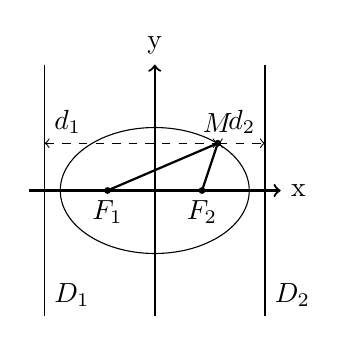
\begin{tikzpicture}[scale=0.4]
			\draw[->, thick] (-4,0) -- (4,0)node[right]{x};
			\draw[->, thick] (0,-4) -- (0,4)node[above]{y};
		
			\draw (0,0) ellipse (3cm and 2cm);
			
			\draw (-3.5,4) -- (-3.5,-4)node[above right]{$D_1$};
			\draw (3.5,4) -- (3.5,-4)node[above right]{$D_2$};
			\draw[thick] (-1.5,0)circle(2pt)node[below]{$F_1$} -- (2,1.5)circle(2pt)node[above]{$M$} -- (1.5,0)circle(2pt)node[below]{$F_2$};
			\draw[dashed, <->] (-3.5,1.5)node[above right]{$d_1$} -- (2,1.5);
			\draw[dashed, <->] (2,1.5) -- (3.5,1.5)node[above left]{$d_2$};
		\end{tikzpicture}
		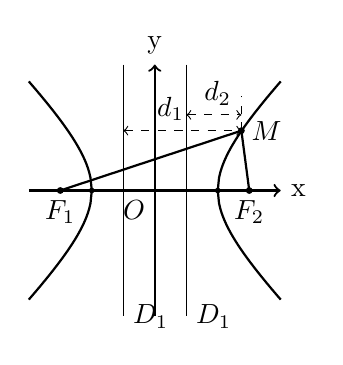
\begin{tikzpicture}[scale=0.4]
			\draw[->, thick] (-4,0) -- (4,0)node[right]{x};
			\draw[->, thick] (0,-4) -- (0,4)node[above]{y};
			%\draw[gray, dashed] (-4,-4) grid (4,4);
		
			\def\a{2};
			\def\b{2};
		
			\draw[domain=\a:4, samples=50, thick] plot (\x,{(\b/\a)*sqrt(\x^2 - \a^2)});
			\draw[domain=\a:4, samples=50, thick] plot (\x,{-(\b/\a)*sqrt(\x^2 - \a^2)});
			\draw[domain=\a:4, samples=50, thick] plot ({-\x},{(\b/\a)*sqrt(\x^2 - \a^2)});
			\draw[domain=\a:4, samples=50, thick] plot ({-\x},{-(\b/\a)*sqrt(\x^2 - \a^2)});
			
			\filldraw[black] (2,0) circle(2pt);
			\filldraw[black] (-2,0) circle(2pt);
			
			\draw (-1,4) -- (-1,-4)node[right]{$D_1$};
			\draw (1,4) -- (1,-4)node[right]{$D_1$};
			%\draw (-3,0)node[below]{$F_1$} -- (2.75,2)node[right]{$M$} -- (3,0)node[below]{$F_2$};
			\filldraw[black, thick] (-3,0)circle(2pt)node[below]{$F_1$} -- (2.75,1.9)circle(2pt)node[right]{$M$} -- (3,0)circle(2pt)node[below]{$F_2$};

			\draw (0,0)node[below left]{$O$};
			
			\draw[dashed] (2.75,1.9) -- (2.75,3);
			
			\draw[dashed, <->] (-1,1.9) -- (0.5,1.9)node[above]{$d_1$} -- (2.75,1.9);
			\draw[dashed, <->] (1,2.4) -- (2,2.4)node[above]{$d_2$} -- (2.75,2.4);
		\end{tikzpicture}
	\end{center}
	
\end{proof}

\begin{remark}
	 Для довільної точки параболи $\dfrac{r}{d} = 1$, тобто $\epsilon = 1$. 
\end{remark}

\subsection{Рівняння дотичної до кривої другого порядку}

Побудуємо рівняння дотичної до еліпса $\dfrac{x^2}{a^2} + \dfrac{y^2}{b^2} = 1$ в точці $M_0(x_0,y_0)$.
Нехай $y_0 \neq 0$, тобто точка $M_0$ не співпадає ні з однією з вершин еліпса $A_1(-a,0)$
та $A_2(a,0)$. У цьому випадку рівняння $\dfrac{x^2}{a^2} + \dfrac{y^2}{b^2} = 1$ неявно задає функцію $y = y(x)$,
$-a < x < a$, графік якої проходить через точку $M_0(x_0,y_0)$ і співпадає з верхньою
(при $y_0 > 0$) чи нижньою (при $y_0 < 0$) половиною еліпса.

Скористаємось відомим із шкільного курсу рівнянням дотичної до графіка
функції $y = f(x)$ в точці з абсцисою $x_0$, яке має вигляд: $y = y_0 + f'(x_0)(x - x_0)$.

Якщо продиференціювати за $x$ тотожність $\dfrac{x^2}{a^2} + \dfrac{y^2(x)}{b^2} = 1$, то отримаємо
рівняння 

$$\dfrac{2x}{a^2} + \dfrac{2yy'(x)}{b^2} = 0,$$ 

\begin{center}
або
\end{center}

$$b^2x + a^2yy'(x) = 0,$$

\begin{center}
тобто 
\end{center}

$$y'(x) = -\dfrac{b^2x}{a^2y}.$$

Якщо підставити значення $y'(x_0) = -\dfrac{b^2x_0}{a^2y_0}$
у рівняння дотичної, то отримаємо рівняння:

$$y = y_0 -\dfrac{b^2x_0}{a^2y_0}(x - x_0).$$

Виконаємо нескладні перетворення:

$$y = y_0 -\dfrac{b^2x_0x}{a^2y_0} +\dfrac{b^2x_0^2}{a^2y_0}, a^2y_0y = a^2y_0^2 - b^2x_0x + b^2x_0^2.$$

Якщо поділити обидві частини рівняння на $a^2b^2$ та врахувати те, що
$\dfrac{x_0^2}{a^2} + \dfrac{y_0^2}{b^2} = 1$ (точка $M_0(x_0,y_0)$ лежить на еліпсі), то отримаємо:

$$\dfrac{y_0y}{b^2} = \dfrac{y_0^2}{b^2} - \dfrac{x_0x}{a^2} + \dfrac{x_0^2}{a^2}.$$

Звідси рівняння дотичної до еліпса в точці $M_0(x_0,y_0)$ має вигляд:

$$\dfrac{x_0x}{a^2} + \dfrac{y_0y}{b^2} = 1.$$

Аналогічно можна вивести рівняння дотичної, проведеної до гіперболи та
параболи в точці $M_0(x_0,y_0)$, відповідно: 

$$\dfrac{x_0x}{a^2} - \dfrac{y_0y}{b^2} = 1,$$

$$yy_0 = p(x + x_0).$$

\section{Комплексні числа}


\subsection{Комплексні числа}

\begin{definition}[Комплексне число]
	\textbf{Комплексне число} -- це впорядкована пара дійсних чисел
	(компонент), для яких поняття рівності, суми, добутку вводяться наступним чином.
\end{definition}

\begin{enumerate}
	\item Нехай $z_1 = (x_1,y_1)$, $z_2 = (x_2,y_2)$. Тоді $z_1 = z_2 \Leftrightarrow x_1 = x_2, y_1 = y_2$.
	
	\item Сума комплексних чисел $z_1$ та $z_2$ -- це впорядкована пара $(x_1 + x_2,y_1 + y_2)$,
	тобто $z_1 + z_2 = (x_1 + x_2,y_1 + y_2)$.

	\item Добуток комплексних чисел $z_1$ та $z_2$ -- це впорядкована пара
	$(x_1x_2 - y_1y_2,x_1y_2 + x_2y_1)$, тобто $z_1z_2 = (x_1x_2 - y_1y_2,x_1y_2 + x_2y_1)$.

	\item Пара $(x,0)$ ототожнюється з дійсним числом $x$, тобто $(x,0) = x$.
\end{enumerate}

Легко перевірити, що всі властивості цих операцій (комутативність,
асоціативність, дис\-три\-бу\-тив\-ність) виконуються.

\underline{Геометрична інтерпретація комплексних чисел.}

Відомо, що дійсні числа відображаються точками числової осі. Встановимо
взаємно однозначну відповідність між множиною комплексних чисел і множиною
точок координатної площини. Комплексному числу $z = (x,y)$ поставимо у
відповідність точку $M(x,y)$ координатної площини $XOY$. Сама координатна
площина -- це комплексна площина. Вісь абсцис -- це дійсна
вісь, вісь ординат -- уявна вісь. Нехай $z = (x,y)$ -- комплексне число, $x$ -- це
його дійсна частина, y – уявна частина (позначають $x = \text{Re}z$, $y = \text{Im}z$).

Комплексне число $z = (x,y)$ також можна інтерпретувати як вектор, початком
якого є точка $O(0,0)$, а кінцем точка $M(x,y)$. Зображення комплексних чисел
векторами дозволяє дати наочну геометричну інтерпретацію операцій над
комплексними числами (додавання, віднімання, множення на константу).

Аналогічно, як у векторній алгебрі, вводиться поняття модуля комплексного
числа $|z| = \sqrt{x^2 + y^2}$, операція множення $z$ на константу: $\alpha z = (\alpha x,\alpha y)$ для
будь-якого $\alpha \in \mathbb{R}$. Модуль числа $z$ дорівнює відстані від початку координат до
точки $M$, яка зображає дане число.

Із визначення комплексного числа випливає, що довільне комплексне число
$z = (x,y)$ може бути записане таким чином:

$$(x,y) = z = (x,0) + (0,1)(0,y).$$

Комплексне число $(x,0)$ ототожнюється з дійсним числом $x$, число $(0, 1)$
позначають символом $i$ (його називають уявною одиницею). Тоді вищенаведена
рівність має вигляд $z = x + iy$. та називається алгебраїчною формою комплексного
числа $z$. Також за означенням $i^2 = ii = (0,1)(0,1) = -1$.

\parbox{3cm}{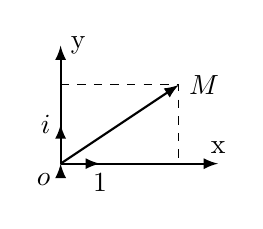
\begin{tikzpicture}[scale=0.5]
	\draw[-latex, thick] (0,0) -- (4,0)node[above]{x};
	\draw[-latex, thick] (0,0) -- (0,3)node[right]{y};
	\draw[-latex, thick] (0,0)node[below left]{$o$};
	
	\draw[-latex, thick] (0,0) -- (0,1)node[left]{$i$};
	\draw[-latex, thick] (0,0) -- (1,0)node[below]{$1$};
	\draw[-latex, thick] (0,0) -- (3,2)node[right]{$M$};
	\draw[dashed] (0,2) -- (3,2) -- (3,0);
\end{tikzpicture}}
\parbox{9cm}{
	Згідно з теорією векторів на площині
	вектори $1=(1,0)$ та $i = (0,1)$ можуть
	слугувати базисом, тоді алгебраїчна форма
	комплексного числа $z$ є саме розкладом $z$
	за цим базисом: $z = x1 + yi$, де $i^2 = -1$.
}

\begin{definition}[Спряжене комплексне число]
	Комплексне число $x - iy$ називається спряженим до комплексного
	числа $z = x + iy$. та позначається символом $\overline{z}$, тобто $\overline{z} = x - iy$.
\end{definition}

Зазначимо, що числу $\overline{z}$ на координатній площині відповідає точка,
симетрична точці $z$ відносно дійсної осі.

\underline{Властивості спряжених чисел}

\begin{enumerate}
	\item $\overline{z_1+z_2} = \overline{z_1} + \overline{z_2}$.
	\item $z + \overline{z} = 2 \text{Re}z$.
	\item $|\overline{z}| = |z|$.
	\item $\overline{z_1z_2} = \overline{z_1}\overline{z_2}$.
	\item $z\overline{z} = |z|^2$.
	\item $z = \overline{z} \Leftrightarrow z \in \mathbb{R}$.
\end{enumerate}

Поділити одне комплексне число $z_1$ на інше комплексне число $z_2$ означає, що
потрібно знайти таке комплексне число $z$, що $z_1 = z_2z$. На практиці ділення 
комплексних чисел виконують за допомогою операції множення: домножують
чисельник і знаменник на число, спряжене знаменнику.

$$\text{Приклад: }\dfrac{1-i}{1+i} = \dfrac{(1-i)^2}{(1-i)(1+i)} = \dfrac{1 - 2i + i^2}{1-i^2} = -\dfrac{2i}{2} = -i.$$

Асоціативний закон множення дозволяє ввести поняття натурального степеня
комплексного числа: $z^n = \underbrace{z \cdot z \cdot ... \cdot z}\limits_n$. За угодою $z^0 = 1$.

Запишемо степені уявної одиниці: $i^0 = 1$, $i^1 = i$, $i^2 = -1$, $i^3 = -i$, $i^4 = 1$.

Останню рівність використовуємо при обчисленні довільних степенів уявної
одиниці.

Приклад: $i^{19} = i^{16 + 3} = i^{16} i^{3} = (i^4)^4i^3 = i^3$.

Множина комплексних чисел позначається $\mathbb{C}$. Очевидно, що множина
дійсних чисел є підмножиною $\mathbb{C}$.

\subsection{Тригонометрична форма комплексного числа}

Нехай $z \in \mathbb{C}$ і $z \neq 0$.

\begin{definition}[Аргументом комплексного числа]
	Кут $\varphi$ між вектором $z$ і ортом дійсної осі називається аргументом
	комплексного числа $z$ і позначається $\text{Arg}z = \varphi$.
\end{definition}

\parbox{3cm}{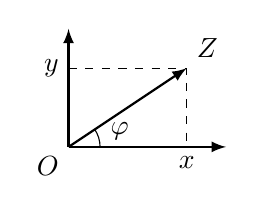
\begin{tikzpicture}[scale=0.5]
	\draw[-latex, thick] (0,0) -- (4,0);
	\draw[-latex, thick] (0,0) -- (0,3);
	\draw (0,0)node[below left]{$O$};
	
	\draw[-latex, thick] (0,0) -- (3,2)node[above right]{$Z$};
	\draw[black] (0.8,0) arc (0:34:0.8);
	\draw (1.3,0.4)node{$\varphi$};	
	\draw[dashed] (0,2)node[left]{$y$} -- (3,2) -- (3,0)node[below]{$x$};
\end{tikzpicture}}
\parbox{9cm}{
Аргумент визначається неоднозначно з точністю до $2\pi$.
Приймаючи до уваги зв'язок між декартовими і
полярними координатами площини $\mathbb{R}^2$, маємо:

$$\begin{array}{l}
    \cos \varphi = \dfrac{x}{\sqrt{x^2 + y^2}} \\
    \sin \varphi = \dfrac{y}{\sqrt{x^2 + y^2}} \\
\end{array}\text{ і }|z| = \sqrt{x^2 + y^2}\text{ або }\begin{array}{l}
    x = |z|\cos\varphi \\
    y = |z|\sin\varphi \\
\end{array}$$
}


Тоді комплексне число $z =x +iy$. можна записати таким чином:
$z = x = |z|(\cos\varphi + i\sin\varphi)$. Ця рівність і називається тригонометричною формою
комплексного числа $z$. 

\begin{problem}[Записати в тригонометричній формі задане комплексне число]
    Записати в тригонометричній формі комплексне число $z = 1 + i$.
\end{problem}
\begin{solution}
    $|z| = \sqrt{1^2 + 1^2} = \sqrt{2}$, $\tg\varphi = \frac{1}{1} = 1$, $\varphi = \frac{\pi}{4}$, оскільки число $z$
    лежить у першій чверті. Отже, $z = 1 + i = \sqrt{2}(\cos\frac{\pi}{4} + i\sin\frac{\pi}{4})$.
\end{solution}

Зауважимо, що дійсні числа теж можна представити як комплексні числа в
тригонометричній формі: $2 = 2(\cos 0 + i\sin 0)$, $-1 = 1(\cos \pi + i\sin \pi)$. 

\section{Многочлени}


\subsection{Алгебра многочленів}

\begin{definition}[Поліномом]
    Многочленом (або поліномом) степені $n$ $(n \geqslant 0, n \in \mathbb{Z})$ від змінної $x$
    називається вираз вигляду $f(x) = a_0x^n + a_1x^{n-1} + ... + a_{n-1}x + a_n = \sum\limits_{k = 0}^n a_kx^{n-k}$, де
    $a_i \in \mathbb{C}, i = 0, ..., n$, причому $a_0 \neq 0$.
\end{definition}

Многочлен нульової степені -- це просто константи. Вводиться нульовий
многочлен: $0(x) = 0x^n + 0x^{n-1} + ... + 0x + 0$. Множину многочленів
степені $\leqslant n$ будемо позначати $P_n$.

\subsection{Операції над многочленами}

Нехай $g(x) \in P_n$: $g(x) = b_0x^n + b_1x^{n-1} + ... + b_{n-1}x + b_n$. Два
многочлени $f(x)$ та $g(x)$ вважаються рівними, якщо в них рівні коефіцієнти при
однакових степенях, тобто, $a_i = b_i$, $i = 0, ..., n$.


1) Множення многочлена на константу $\alpha \in \mathbb{C}$:

$$(\alpha f)(x) = \alpha\sum\limits_{k=0}^n a_k x^{n-k} = \sum\limits_{k=0}^n (\alpha a_k) x^{n-k}.$$

2) Додавання многочленів $f(x)$ та $g(x)$:

$$(f + g)(x) = \alpha\sum\limits_{k=0}^n (a_k+b_k)x^{n-k}.$$

Нехай $f, g, p \in P_n$, константи $\alpha, \beta \in \mathbb{C}$. Операції множення та додавання
мають наступні властивості.
 
\begin{enumerate}
    \item $f + g = g + f$.
    \item $f + (g + p) = (f + g) + p$.
    \item $(\alpha\beta)f = \alpha(\beta f)$.
    \item $(\alpha + \beta)f = \alpha f + \beta f$.
    \item $\alpha(f + g) = \alpha f + \alpha g$.
    \item Існує нульовий многочлен $0(x) \in P_n$: $f(x) + 0(x) = f(x)$.
    \item Для будь-якого многочлена $f(x)$ існує протилежний многочлен -- $f(x)$, такий що $f(x) + (-f)(x) = 0(x)$.
    \item $1 \cdot f(x0 = f(x)$; $(-f)(x) = (-1)f(x)$.
\end{enumerate}

3) Множення многочленів $f(x)$ та $g(x)$: щоб помножити многочлен $f(x)$ на
многочлен $g(x)$, потрібно кожний член многочлена $f(x)$ помножити на кожний
член $g(x)$, додати отримані добутки і звести подібні члени. Степінь добутку двох
многочленів дорівнює завжди сумі степенів множників.

4) Ділення многочленів $f(x)$ на $g(x)$ ($g(x) \neq 0$) з остачею. Позначимо
$\deg g(x)$ -- степінь многочлена $g(x)$.

\begin{theorem}
    Для двох довільних многочленів $f(x)$ та $g(x)$ знайдуться
    многочлени $p(x)$ і $r(x)$ такі, що
    
    $$f(x) = g(x)p(x) + r(x)$$
    
    де $\deg r(x) < \deg g(x)$ і таке представлення єдине.
    
    Многочлен $p(x)$ називається часткою, а $r(x)$ -- остачею від ділення
    многочлена $f(x)$ на $g(x)$.
\end{theorem}
\begin{proof}
    Нехай $f(x) = a_0x^n + a_1x^{n-1} + ... + a_{n-1}x + a_n$, $\deg f(x) = n$,
    $g(x) = b_0x^m + b_1x^{m-1} + ... + a_m$, $\deg g(x) = m$. Розглянемо два випадки:
    
    1) $m > n: f(x) = g(x) 0(x) + f(x)$, тобто частка -- нульовий многочлен, а остача
    --- це $f(x)$; 
    
    2) $n \geqslant m$: ділимо “кутом” многочлен $f(x)$ на $g(x)$ (відомо зі шкільного курсу
    алгебри); тоді $f(x) = g(x)p(x) + r(x)$, де $p(x)$ -- частка та $r(x)$ -- остача від
    ділення.
    
    Єдиність представлення доводимо від супротивного. Припустимо, що існує інший
    розклад, відмінний від даного: $f(x) = g(x)\tilde{p}(x) + \tilde{r}(x)$. Віднімемо ці розклади. Тоді
    \begin{equation*}
        0 = g(x)(p(x) -\tilde{p}(x)) + r(x) - \tilde{r}(x),
    \end{equation*}
    \begin{equation*}
        g(x)(p(x) -\tilde{p}(x)) = \tilde{r}(x) - r(x). (**).
    \end{equation*}
    З останньої рівності випливає, що
    \begin{equation*}
        \deg g(x) + \deg(p(x) -\tilde{p}(x)) = \deg(\tilde{r}(x) - r(x)).
    \end{equation*}
    Оскільки степінь многочлена $\tilde{r}(x) - r(x)$ менша степені $g(x)$, то рівність $(**)$
    можлива лише тоді, коли $p(x) -\tilde{p}(x) = 0$. Це означає, що $p(x) = \tilde{p}(x)$ та $r(x) = \tilde{r}(x)$,
    що доводить єдиність розкладу (*).
\end{proof}

\begin{remark}
    Якщо $r(x) = 0$, то кажуть, що $f(x)$ ділиться на $g(x)$ без остачі (націло)
    і позначають: $f(x) \divby g(x)$.
\end{remark}

\begin{claim}
	$f(x) \divby g(x) \Rightarrow \alpha f(x) \divby g(x)$, де $\alpha = const$.
\end{claim}

\begin{claim}
	$f(x) \divby g(x)$ та $q(x) \divby g(x) \Rightarrow \alpha f(x) + \beta q(x) \divby g(x)$,
	де $\alpha, \beta = const$. 
\end{claim}

\subsection{Найбільший спільний дільник двох многочленів}

\begin{definition}[Спільний дільник]
	Якщо кожен з многочленів $f(x)$ та $g(x)$ ділиться без остачі на
	многочлен $\varphi(x)$, то $\varphi(x)$ називається спільним дільником $f(x)$ і $g(x)$.
\end{definition}

\begin{definition}[Найбільший спільний дільник]
	Найбільшим спільним дільником (НСД) многочленів $f(x)$ та $g(x)$
	називається такий їх спільний дільник $d(x)$, який ділиться на всі інші спільні
	дільники многочленів і позначається $(f(x),g(x)) = d(x)$.
\end{definition}

Для будь-яких двох многочленів, які не дорівнюють одночасно нулю, НСД
існує і визначається однозначно з точністю до множників-констант. Із усіх НСД
вибирається той, у якого старший коефіцієнт дорівнює 1.

\begin{definition}[Взаємно прості поліноми] 
	Два многочлени $f(x)$ та $g(x)$ називаються взаємно простими, якщо $(f,g) = 1$.
\end{definition}

Якщо відомі розклади многочленів $f(x)$ та $g(x)$ на лінійні множники, то НСД
$(f,g)$ легко знаходяться. Справді, нехай

$$f(x) = a_0(x-\alpha_{1})^{k_1}...(x-\alpha_{p})^{k_p}(x-\beta_{1})^{n_1}...(x-\beta_{l})^{n_l},$$

$$f(x) = a_0(x-\alpha_{1})^{i_1}...(x-\alpha_{p})^{i_p}(x-\gamma_{1})^{m_1}...(x-\gamma_{s})^{m_s},$$

де числа $\alpha_j, \beta_j, \gamma_j$ є попарно різними. Тоді

$$(f,g) = (x-\alpha_1)^{\min(k_1,i_1)}...(x-\alpha_p)^{\min(k_p,i_p)}$$

Якщо ж розклад многочленів на множники невідомий, то для знаходження
НСД використовують алгоритм Евкліда. 

\subsection{Алгоритм Евкліда}

Нехай $\deg f(x) \geqslant \deg g(x)$. За теоремою про ділення многочленів з остачею:

$$f(x) = g(x)p_1(x) + r_1(x), \deg r_1(x) < \deg g(x);$$

$$g(x) = r_1(x)p_2(x) + r_2(x), \deg r_2(x) < \deg r_1(x);$$

$$r_1(x) = r_2(x)p_3(x) + r_3(x), \deg r_3(x) < \deg r_2(x);$$

$$...$$

$$r_{k-2}(x) = r_{k-1}(x)p_k(x) + r_k(x), \deg r_k(x) < \deg r_{k-1}(x);$$

$$r_{k-1}(x) = r_{k}(x)p_{k+1}(x) + r_{k+1}(x), \deg r_{k+1}(x) < \deg r_{k}(x);$$

$$r_{k}(x) = r_{k+1}(x)p_{k+2}(x);$$

$$d(x) = r_{k+1}(x).$$

Остання ненульова остача $r_{k+1}(x)$ є НСД многочленів $f(x)$ і $g(x)$.

\begin{problem}[Знайти НСД заданих многочленів]
	Знайти НСД многочленів

	$$f(x) = x^4 + 3x^3 - x^2 - 4x - 3, g(x) = 3x^3 + 10x^2 + 2x -3.$$
\end{problem}

\begin{solution}
    \textit{Розв’язання задачі проводимо за наступною схемою}:
    
    \begin{enumerate}
        \item $f:g$ і знаходимо остачу $r_1$; 
        \item $g:r_1$ і знаходимо остачу $r_2$;
        \item $r_1:r_2$ і знаходимо остачу $r_3$;
        
        \indent \vdots
    
        \item $r_k:r_{k+1}$ (остача 0).
    \end{enumerate}
    
    Ділимо дані многочлени “кутом”, при цьому можна множити ділене та дільник
    на будь-які ненульові числа (навіть у процесі самого ділення). У нашому випадку
    ділимо $3f$ на $g$:
    
    $$x^4 + 3x^3 - x^2 -4x -3 = (3x^3 + 10x^2 + 2x - 3)(x - \dfrac{1}{3}) + (-\dfrac{5}{3}x^2 - \dfrac{25}{3}x - 10)$$
    
    Як $r_1(x)$ обираємо тричлен $x^2 + 5x +6$ (остачу помножили на $-\frac{3}{5}$). Далі
    
    $$3x^3 + 10x^2 + 2x - 3 = (x^2 + 5x + 6)(3x - 5) + (9x + 27)$$
    
    Як $r_2(x)$ обираємо двочлен $x+3$ (остачу помножили на $\frac{1}{9}$). Далі
    
    $$x^2 + 5x + 6 = (x + 3)(x + 2) + 0$$
    
    Шуканим НСД многочленів $f(x)$ та $g(x)$ є остання ненульова остача $r_2(x)$.
    Маємо
    \begin{equation*}
        (f(x), g(x)) = x + 3.
    \end{equation*}
\end{solution}

\subsection{Корені многочленів}

\begin{definition}[Корінь полінома]
	Число $x_0$ називається коренем многочлена $f(x)$, якщо $f(x_0) = 0$.
\end{definition}

\begin{definition}[Кратність кореня полінома]
	Корінь многочлена $x_0$ має кратність $k$, якщо $f(x) = (x-x_0)^k\varphi(x)$,
	причому $\varphi(x) \neq 0$ і $f(x)$ не ділиться на $(x-x_0)^{k+1}$. Корені кратності $k = 1$
	називаються простими коренями многочлена $f(x)$.
\end{definition}

\begin{claim}
	Многочлени $f(x)$ та $g(x)$ є взаємно простими тоді і тільки тоді, коли
	вони не мають жодного спільного кореня.
\end{claim}

\begin{claim}
	Якщо $x_0$ -- корінь кратності $k$ для $f(x)$, то $x_0$ є коренем кратності $k-1$
	для $f'(x)$.
\end{claim}
\begin{proof}
	Якщо $x_0$ -- корінь кратності $k$ для $f(x)$, то $f(x) = (x-x_0)^k\varphi(x), \varphi(x) \neq 0$.
	У цьому випадку $f'(x) = k(x-x_0)^{k-1}\varphi(x) + (x-x_0)^k\varphi'(x) = (x-x_0)^{k-1}(k\varphi(x)
	+ (x-x_0)\varphi'(x)) = (x-x_0)^{k-1}\psi(x)$, де $\psi(x) = k\varphi(x) + (x-x_0)\varphi'(x)$,
	причому $\psi(x_0) = k\varphi(x_0) + 0 \varphi'(x_0) = k\varphi(x_0) \neq 0$.
\end{proof}

\begin{theorem}[Теорема Безу]
	Остача від ділення многочлена $f(x)$ на $x-b$ дорівнює $f(b)$.
\end{theorem}
\begin{proof}
	Многочлен $f(x)$ можна подати у вигляді $f(x) =  (x-b)p(x) + r$,
	де $r = const$. Тому $f(b) = r$.
\end{proof}

\begin{corollary}
	Якщо $x_0$ -- корінь многочлена $f(x)$, то остача від ділення $f(x)$ на
	$(x - x_0)$ дорівнює нулю.
\end{corollary}
\begin{proof}
	Доведення. Очевидно, що $r = f(x_0) = 0$. 
\end{proof}

\subsection{Основна теорема алгебри та її наслідки}

\begin{theorem}
	Будь-який многочлен $f(x)$ ненульової степені з комплексними чи
	дійсними коефіцієнтами має принаймні один дійсний чи комплексний корінь.
\end{theorem}

\begin{corollary}
	Будь-який многочлен $f(x)$ $n$-ої степені $(n \geqslant 1)$ має рівно $n$ коренів.
\end{corollary}
\begin{proof}
	Нехай $\deg f(x) = n$, тоді за основною теоремою алгебри $x_1$ -- це
	корінь многочлена $f(x)$. Маємо $f(x_1) = 0$, тобто $f(x) = (x - x_1)g_1(x)$, причому
	$\deg g_1(x) = n-1$. Якщо $n - 1 \geqslant 1$, то многочлен $g_1(x)$ має хоча б один корінь $x_2$:
	$g_1(x_2) = 0$ і $g_1(x) = (x - x_2)g_2(x)$. Повторивши аналогічні міркування потрібну
	кількість разів, отримаємо розклад многочлена $f(x)$ на лінійні множники:
	$f(x) = a_0(x-x_1)(x-x_2)...(x-x_n)$,
	а це і означає, що даний многочлен має рівно n коренів.
\end{proof}

\begin{corollary}
	Кожний многочлен $f(x)$ можна представити у вигляді:
	$f(x) = a_0(x-x_1)^{\alpha_1}(x-x_2)^{\alpha_2}...(x-x_s)^{\alpha_s}$,
	де $x_i$ -- корінь кратності $\alpha_i$, причому $\alpha_1 + \alpha_2 + ... + \alpha_s = n = \deg f(x)$ і цей розклад
	є єдиним (з точністю до порядку множників).
\end{corollary}

\begin{corollary}
	Якщо $f(x)$ і $g(x)$ -- многочлени степені $n$ і їх значення
	співпадають в $(n+1)$ різних точках, то $f(x) \equiv g(x)$.
\end{corollary}
\begin{proof}
	Нехай існують такі значення $x_1 < ... < x_{n+1}$, що $f(x_k) = g(x_k)$,
	$k = 1, ..., n+1$. Розглянемо многочлен $F(x) = f(x) - g(x)$. Очевидно, що
	$\deg F(x) \leqslant n$ і $F(x_1) = ... = F(x_{n+1} = 0)$, тобто $x_k$, $k = 1, ..., n+1$, є коренями
	многочлена $F(x)$. Таким чином, многочлен степені $\leqslant n$ має $n+1$ корінь, а це
	суперечить наслідку 1 основної теореми алгебри. Отже, $F(x) \equiv 0$, а це означає, що
	$f(x) \equiv g(x)$.
\end{proof}

\begin{corollary}
	Якщо число $z_0$ -- це комплексний корінь многочлена $f(x)$ з
	дійсними коефіцієнтами, то $\overline{z_0}$ є також коренем цього многочлена, причому їх
	кратності співпадають. 
\end{corollary}
\begin{proof}
	Нехай $z_0$ -- це комплексний корінь многочлена з дійсними
	коефіцієнтами $f(x) = a_0x^n + a_1x^{n-1} + ... + a_{n-1}x + a_n$. Тоді $f(z_0) = 0$. Оскільки
	$a_i \in \mathbb{R}$, то $a_i = \overline{a_i}$, $i = 0, 1, ..., n$. Доведемо,
	що $f(\overline{z_0}) = 0$, використовуючи
	властивості комплексно спряжених чисел:
	
	$$f(\overline{z_0}) = a_0(\overline{z_0})^n + ... + a_{n-1}\overline{z_0} + a_n = a_0\overline{z_0^n} + ... + a_{n-1}\overline{z_0} + a_n =$$
	
	$$= \overline{a_0}\overline{z_0^n} + ... + \overline{a_{n-1}}\overline{z_0} + \overline{a_n} = \overline{a_0 z_0^n} + ... + \overline{a_{n-1}z_0} + \overline{a_n} = \overline{a_0z_0^n + ... + a_{n-1}z_0 + a_n} =$$
	
	$$= \overline{f(z_0)} = \overline{0} = 0.$$
\end{proof}

\begin{corollary}
	Довільний многочлен з дійсними коефіцієнтами можна
	представити у вигляді добутку многочленів з дійсними коефіцієнтами степені, не
	вище другої.
\end{corollary}
\begin{proof}
	Довільний многочлен $f(x)$ може мати як дійсні, так і комплексні
	корені. Нехай $x_1, ..., x_s$ -- його дійсні корені кратності $\alpha_1, ..., \alpha_s$ відповідно,
	а $z_1, ..., z_t$ -- комплексні корені кратності $\beta_1, ..., \beta_t$. Згідно з наслідком 4 комплексно спряжені
	числа $\overline{z_1}, ..., \overline{z_t}$ теж будуть коренями многочлена $f(x)$ відповідної кратності. Отже,
	даний многочлен буде ділитись на $(x - x_i)^{\alpha_i}$, $i = 1, ..., s$, без остачі. Аналогічно
	$f(x)$ буде ділитись без остачі на $(x - z_j)^{\beta_j} (x - \overline{z_j})^{\beta_j}$, 
	$j = 1, ..., t$. Отже, маємо:
	
	$$(x - z_j)^{\beta_j} (x - \overline{z_j})^{\beta_j} = ((x - z_j)(x - \overline{z_j}))^{\beta_j} = (x^2 - (z_j + \overline{z_j})x + z_j\overline{z_j})^{\beta_j} =$$
	
	$$x^2 - 2(\text{Re}z)x + |z_j|^2 = x^2 - 2a_jx + b_j$$	
		
	де $a_j, b_j \in \mathbb{R}$. Тому
	
	$$f(x) = a_0(x-x_1)^{\alpha_1} ... (x-x_s)^{\alpha_s} (x^2 + a_1x + b_1)^{\beta_1} ... (x^2 + a_tx + b_t)^{\beta_t}$$	

	причому $\alpha_1 + ... + \alpha_s + 2(\beta_1 + ... + \beta_t) = n$. 
\end{proof}

\section{Лінійний простір}  %p 59


\subsection{Лінійний простір}

Розглянемо різні об’єкти: вектори, многочлени, комплексні числа. Над ними
були визначені лінійні операції: множення на константу і додавання. Залежно від 
природи цих об’єктів операції задавались по-різному, але вони задовольняли одним
і тим самим законам (асоціативність, комутативність та дистрибутивність).

Якщо залишити осторонь природу конкретних об’єктів і ввести аксіоматично
визначені дві операції, які мають певні властивості, то можна побудувати загальну
теорію, що узагальнює конкретні випадки. Таким чином і виникло поняття
лінійного простору як безпосереднє узагальнення дво- та тривимірних векторних
просторів.

Нехай $K$ -- це множина дійсних чисел (або комплексних чисел), тобто $k = \mathbb{R}$
або $k = \mathbb{C}, L \neq \varnothing$. 

\begin{definition}[Лінійний простір $L$ над полем $K$]
	\textbf{Лінійний простір $L$ над полем $K$} -- це множина деяких
	елементів, на якій введено операції додавання і множення на скаляр, які не
	виводять за межі $L : x, y \in L, \alpha \ in K \Rightarrow x + y \in L, \alpha x \in L$. Для будь-яких
	елементів $x, y, z \in L$ і будь-яких чисел $\alpha, \beta \in K$ виконуються такі аксіоми:
	\begin{enumerate}
		\item $x + y = y + x$ -- комутативність додавання;
		\item $(x+y)+z = x+(y+z)$ -- асоціативність додавання;
		\item $(\alpha \beta)x = \alpha (\beta x)$ -- асоціативність множення на скаляр;
		\item $(\alpha + \beta)x = \alpha x + \beta x$ -- дистрибутивність відносно скалярів;
		\item $\alpha(x + y) = \alpha x + \alpha y)$ -- дистрибутивність відносно векторів;
		\item існує нульовий елемент $\overline{0} \in L: x + \overline{0} = x$;
		\item $\forall x \in L \: \exists x'$ -- протилежний елемент, такий що $x + x' = \overline{0}$;
		\item $1 x = x$.
	\end{enumerate}
\end{definition}

Елемент лінійного простору -- це \textbf{вектор}, сам простір ---
\textbf{векторний простір}. Лінійний простір -- це \textbf{дійсний простір}, якщо $k = \mathbb{R}$,
а якщо $k = \mathbb{C}$, то це -- \textbf{комплексний простір}.

\begin{remark}
	Символом $\overline{0}$ будемо позначати нульовий вектор лінійного
	простору, а символом 0 -- дійсне число -- нуль.
\end{remark}

Прикладами лінійного простору може слугувати множина дійсних чисел $\mathbb{R}$,
множина комплексних чисел $\mathbb{C}$, множина векторів на площині $E^2$, множина 
векторів у просторі $E^3$. Множина $C_{[a,b]}$ всіх неперервних функцій $f(x)$, які
визначені на відрізку $[a,b]$, з поточковим додаванням і множенням на константу, а
також множина многочленів $P_n$ степені $\leqslant n$ теж є лінійними просторами.

\textit{Властивості лінійного простору}
\begin{enumerate}
	\item В довільному лінійному просторі існує єдиний нульовий елемент.
	\item В довільному лінійному просторі для будь-якого елемента існує єдиний обернений.
	\item В довільному лінійному просторі $0 x = \overline{0}$, а протилежний елемент $x' = (-1)x$.
\end{enumerate}
\begin{proof}
	$$0x = 0 x + \overline{0} = 0 x + (x+x') = (0x + x) + x' = (0x + 1x) + x' = $$
	
	$$= (0 + 1)x + x' = 1x + x' = x + x' = \overline{0}.$$
\end{proof}

\begin{example}
	Проведемо узагальнення поняття вектора. Нехай $x = \begin{pmatrix}
		x_1  \\
		\vdots  \\
		x_n  \\
	\end{pmatrix}$ -- це
	впорядкована множина з $n$ дійсних чисел, записаних у стовпчик (вектор).
	Множину векторів такого виду позначимо $\mathbb{R}^n = \left\{\left.\begin{pmatrix}
		x_1  \\
		\vdots  \\
		x_n  \\
	\end{pmatrix}\right| x_i \in \mathbb{R}\right\}$. Доведемо, що $\mathbb{R}^n$
	є лінійним простором.
\end{example}
\begin{proof}
	Нехай $y \in \mathbb{R}^n$, тобто $y = \begin{pmatrix}
		y_1  \\
		\vdots  \\
		y_n  \\
	\end{pmatrix}, y_i \in \mathbb{R}m i = \overline{1, n}$, i $\alpha \in \mathbb{R}$. Тоді
	природньо ввести операції додавання та множення на скаляр таким чином:
		
	 $$x + y = \begin{pmatrix}
		x_1 + y_1  \\
		\vdots  \\
		x_n + y_n  \\
	\end{pmatrix}, \alpha x = \begin{pmatrix}
		\alpha x_1  \\
		\vdots  \\
		\alpha x_n  \\
	\end{pmatrix}.$$
	
	Окрім того, задамо вектор, протилежний до $x$, та нульовий вектор:
	
	$$x' =\begin{pmatrix}
		-x_1  \\
		\vdots  \\
		-x_n  \\
	\end{pmatrix}, \overline{0} = \begin{pmatrix}
		0  \\
		\vdots  \\
		0  \\
	\end{pmatrix}.$$

	Очевидно, що для заданих таким чином векторів і операцій додавання та
	множення на константу, виконуються всі аксіоми лінійного простору. Отже, $\mathbb{R}^n$ ---
	це лінійний простір, який називають арифметичним. 
\end{proof}

\subsection{Матриці як приклад лінійного простору}

\begin{definition}[Матриця]
	Матрицею розмірів $n$ на $m$ називається сукупність $n \times m$ чисел,
	записаних у вигляді прямокутної таблиці, що містить $n$ рядків та $m$ стовпчиків.
\end{definition}

Вектор-стовпчик можна розглядати, як матрицю $n \times 1$, матриця $1 \times n$ -- це
вектор-рядок.

Розглянемо множину матриць $M_{n \times m}, A, B, C \in M_{n \times m}$,

$$A = (a_{ij}), B = (b_{ij}), C = (c_{ij}), i = \overline{1,n},j = \overline{1,m}.$$

\begin{definition}[Рівність матриць]
	$A = B \Leftrightarrow a_{ij} = b_{ij}, \forall i, j$.
\end{definition}

\begin{definition}[Сума матриць]
	\textbf{Сума матриць $A$ і $B$} -- це матриця $C = A + B$, елементи
	якої дорівнюють сумі відповідних елементів матриць $A$ і $B$, тобто $c_{ij} = a_{ij} + b_{ij}$.
\end{definition}

\begin{definition}[Добуток матриць]
	\textbf{Добуток матриці $A$ на число $\alpha$} -- це матриця $B = \alpha A$, кожен
	елемент якої є добутком відповідного елемента даної матриці на число $\alpha$, тобто
	$b_{ij} = \alpha a_{ij}$.
\end{definition}

\begin{definition}[Нульова матриця]
	Матриця називається нульовою, якщо всі її елементи дорівнюють нулю:

	$$O = \begin{pmatrix}
		0 & ... & 0  \\
		\vdots & \ddots & \vdots  \\
		0 & ... & 0  \\
	\end{pmatrix}.$$
\end{definition}

\begin{definition}[Протилежна матриця]
	Матриця $(-1)A = -A$ -- це \textbf{протилежна матриця} до матриці $A$.
\end{definition}

Очевидно, $A + (-A) = O$.

\begin{definition}[Різниця матриць]
	Сума матриць $A$ і $-B$ -- це \textbf{різниця матриць $A$ і $B$} та
	позначається $A - B$. 
\end{definition}

Легко перевірити, що всі аксіоми лінійного простору виконуються, тому
множина матриць із заданими операціями додавання і множення на число є
лінійним простором.

\textit{Множення матриць}

Добуток матриць $A B$ визначається тільки за умови, коли кількість
стовпчиків матриці $A$ дорівнює кількості рядків матриці $B$.

\begin{definition}[Добуток матриць]
	Добуток $A B$ матриць $A = (a_{ij})_{i=\overline{1,n}, j=\overline{1,m}}$ i $B = (b_{jk})_{j=\overline{1,m}, k=\overline{1,p}}$
	називається матриця $C = (c_{ik})_{i=\overline{1,n}, k=\overline{1,p}}$, елементи якої визначаються рівністю:
	$c_{ik} = a_{i1}b_{1k} + a_{i2}b_{2k} + ... + a_{im}b_{mk}, i = \overline{1,n}, k = \overline{1,p}$.
\end{definition}

Таким чином, елемент $c_{ik}$ дорівнює сумі добутків елементів $i$-го рядка
матриці $A$ на відповідні елементи $k$-го стовпчика матриці $B$.

\begin{example}
Приклад. Знайти добуток матриць
$A = \begin{pmatrix}
	2 & -1 \\
	0 & 3 \\
	1 & 0 \\
\end{pmatrix}$ та $B = \begin{pmatrix}
	3 & 1 \\
	0 & -1 \\
\end{pmatrix}$

$C = \begin{pmatrix}
	2 & -1 \\
	0 & 3 \\
	1 & 0 \\
\end{pmatrix} \times \begin{pmatrix}
	3 & 1 \\
	0 & -1 \\
\end{pmatrix} = \begin{pmatrix}
	2 \cdot 3 + (-1) \cdot 0 	& 2 \cdot 1 + (-1) \cdot (-1) \\
	0 \cdot 3 					& 0 \cdot 1 + 3 \cdot (-1) \\
	1 \cdot 3 + 0 \cdot 0 		& 1 \cdot 1 + 0 \cdot (-1) \\
\end{pmatrix} = \begin{pmatrix}
	6 & 3 \\
	0 & -3 \\
	3 & 1 \\
\end{pmatrix}$
\end{example}

Зауважимо, що для даних матриць знайти добуток $B \cdot A$ неможливо.

Якщо ж матриці $A$ і $B$ є квадратними розміру $n \times n$, то можна обчислити $A \cdot B$
та $B \cdot A$. Відзначимо важливу властивість: множення матриць є некомутативним,
тобто $A \cdot B \neq B \cdot A$. Проте існують матриці, які називаються переставними, для
яких виконується рівність $A \cdot B = B \cdot A$.

\begin{definition}[Діагональна матриця]
	Квадратна матриця, у якої всі елементи $a_{ij} = 0$ при $i \neq j$, називається
	діагональною. Якщо ж у діагональній матриці, всі елементи $a_{ii}$ дорівнюють
	одиниці, то матриця називається одиничною і позначається літерою $I$: 
	
	$$I = \begin{pmatrix}
		1 & ... & 0  \\
		 & \ddots &   \\
		 0 & ... & 1  \\
	\end{pmatrix}.$$
\end{definition}

Можна довести, що одинична матриця $I$ є переставною з будь-якою
квадратною матрицею $A$ такого ж розміру: $A I = I A = A$.

\textit{Властивості множення матриць}
\begin{enumerate}
	\item $AB \neq BA$.
	\item $(AB)C = A(BC)$.
	\item $(A+B)C = AC + BC, A(B+C) = AB + AC$.
	\item $\alpha(AB) = (\alpha A)B$.
\end{enumerate}

\textit{Лінійний підпростір}

\begin{definition}[Лінійний підпростір]
	Підмножина $L_1$ лінійного простору $L$ називається лінійним
	підпростором, якщо вона є лінійним простором відносно операцій, введених в $L$.
\end{definition}

\begin{claim}
	$L_1$ є лінійним підпростором $L \Leftrightarrow$
	
	$\Leftrightarrow \begin{array}{l}
		1) \forall x, y \in L_1 : x + y \in L_1  \\
		2) \forall x \in L_1, \alpha \in \mathbb{R} : \alpha x \in L_1  \\
	\end{array}$
\end{claim}

\begin{proof}
	Якщо $L_1$ -- лінійний підпростір $L$ , то умови $1)$ та $2)$ виконуються
	автоматично. Покажемо, що підмножина $L_1$, елементи якої задовольняють умови
	$1)$ та $2)$ є лінійним підпростором. Зауважимо, що всі аксіоми, окрім 6 та 7,
	виконуються, оскільки вони відносяться до будь-яких елементів простору L.
	
	Перевіримо, чи виконуються аксіоми 6 та 7.
	
	Нехай $x \in L_1$. Згідно з умовою $2)$ маємо $\alpha x \in L_1$. Оскільки $\alpha \in \mathbb{R}$ є довільним,
	то при $\alpha = 0$ та $\alpha = -1$ маємо співвідношення: $0x = \overline{0} \in L_1$, $(-1)x = -x \in L_1$. Це
	означає, що в $L_1$ існує нульовий елемент $\overline{0}$ і для довільного $x \in L_1$ існує
	протилежний елемент $x' = -x \in L_1$. Тому аксіоми 6 та 7 також виконуються. Отже,
	$L_1$ є лінійним простором, тобто $L_1$ -- це лінійний підпростір лінійного простору $L$.
\end{proof}

\textit{Приклади лінійних підпросторів:}
\begin{enumerate}
	\item множина ${\overline{0}}$ -- це лінійний підпростір для будь-якого лінійного простору $L$;
	\item множина компланарних векторів $E^2$ є лінійним підпростором простору $E^3$;
	\item множина колінеарних векторів $E^1$ є лінійним підпростором простору $E^2$ і простору $E^3$. 
\end{enumerate}

\subsection{Лінійні оболонки}

Нехай $L$ -- це довільний лінійний простір, $a_1, a_2, ..,a_n \in L$.

\begin{definition}[Лінійна оболонка]
	Лінійною оболонкою векторів $a_1, a_2, ..,a_n$ називається множина всіх
	можливих лінійних комбінацій цих векторів:
	
	$$\Lambda(a_1, a_2, ..,a_n) = \{x \mid x \in L, x = \sum\limits_{i=1}^n \alpha_i a_i, \alpha_i \in K\}$$
\end{definition}

\begin{example}
	\begin{enumerate}
		\item $\overline{a} \in E^3, \overline{a} \neq \overline{0}, \Lambda(\overline{a}) = \{x \mid x \in E^3, x = \alpha \overline{a}\} = E^1$.
		\item Вектори $\overline{a}, \overline{b}$ -- неколінеарні, $\Lambda(\overline{a}, \overline{b}) = \{x \mid x = \alpha \overline{a} + \beta \overline{b}, x \in E^3\} = E^2$.
	\end{enumerate}
\end{example}


\begin{claim}
	Лінійна оболонка довільних векторів $a_1, a_2, ..,a_n$ з $L$ є лінійним
	підпростором цього ж лінійного простору $L : \Lambda(a_1, a_2, ..,a_n) \subset L$.
\end{claim}
\begin{proof}
	Нехай $x, y \in \Lambda(a_1, a_2, ..,a_n)$, тоді $x = \sum\limits_{i=1}^n \alpha_i a_i$,
	$y = \sum\limits_{i=1}^n \beta_i a_i$.
	
	Скористаємось твердженням про лінійний підпростір, доведемо виконання
	двох умов.
	
	$$1) \lambda x = \lambda \sum\limits_{i=1}^n \alpha_i a_i = \sum\limits_{i=1}^n (\lambda \alpha_i) a_i \in \Lambda(a_1, ..., a_n).$$
	
	$$2) x+y = \sum\limits_{i=1}^n \alpha_i a_i + \sum\limits_{i=1}^n \beta a_i = \sum\limits_{i=1}^n (\alpha_i + \beta_i) a_i \in \Lambda(a_1, ..., a_n).$$
\end{proof}

\subsection{Базис і розмірність лінійного простору}

Нехай $L$ -- це довільний лінійний простір, $L \neq \{0\}$. 

\begin{definition}[Базис лінійного простору]
	Базисом лінійного простору $L$ називається максимальна лінійно
	незалежна система векторів (приєднання будь-якого вектора з $L$ перетворює цю
	систему на лінійно залежну). Якщо базис містить $n$ векторів, то лінійний простір
	$L$ називається $n$-вимірним, а число $n$ -- розмірністю лінійного простору і
	позначається $\dim L = n$.
\end{definition}

\begin{remark}
	Якщо $L$ містить лише $\overline{0}$, то $\dim L = 0$.
\end{remark}

\textit{Алгоритм побудови базису формулюється таким чином.}
\begin{enumerate}
	\item Вибираємо довільний вектор $e_1 \in L, e_1 \neq \overline{0}$.
	
	\item Вибираємо довільний вектор $e_2 \in L, e_2 \neq \overline{0}$ таким чином, щоб вектори $e_1$ та
	$e_2$ були лінійно незалежними.
	
	\item Припустимо, що вказана процедура дозволила побудувати лінійно незалежні
	вектори $e_1, e_2, ..., e_n$. Якщо приєднання до $e_1, e_2, ..., e_n$ довільного вектора $b \in L$
	перетворює цю систему векторів на лінійно залежну, то вектори $e_1, e_2, ..., e_n$
	утворюють базис лінійного простору $L$. Тоді $b = \sum\limits_{i=1}^n \alpha_i e_i$ і $b \in \Lambda(e_1, e_2, ..., e_n)$.
\end{enumerate}

\begin{claim}
	Якщо вектори $e_1, e_2, ..., e_n$ є базисом лінійного простору $L$, то
	$\Lambda(e_1, e_2, ..., e_n) = L$.
\end{claim}

\begin{definition}[Повна система  векторів]
	Система векторів простору $L$ називається повною, якщо кожний вектор
	простору $L$ лінійно виражається через вектори цієї системи.
\end{definition}

\begin{definition}[Базис лінійного простору]
	Базисом лінійного простору $L$ називається повна лінійно незалежна
	система векторів.
\end{definition}

Доведемо еквівалентність двох означень базису лінійного простору.
\begin{proof}
	Озн. 1 $\rightarrow$ Озн. 2. Нехай $e_1, e_2, ..., e_n$ -- максимальна лінійно незалежна система
	векторів. Тоді для будь-якого $x \in L$ вектори $e_1, e_2, ..., e_n, x$ є лінійно залежними, і
	можна довести, що $x = \sum\limits_{i=1}^n x_ie_i$. Отже, $e_1, e_2, ..., e_n$ -- це повна
	лінійно незалежна система векторів.

	Озн. 2 $\rightarrow$ Озн. 1. Нехай $e_1, e_2, ..., e_n$ -- це повна лінійно незалежна система
	векторів. Тоді будь-який вектор $x \in L$ можна подати у вигляді $x = \sum\limits_{i=1}^n x_ie_i$, тобто
	$\sum\limits_{i=1}^n x_ie_i + (-1)x = \overline{0}$. Отже, вектори $e_1, e_2, ..., e_n, x$ є лінійно
	залежними. Це означає, що $e_1, e_2, ..., e_n$ -- це максимальна лінійно незалежна система.
\end{proof}

\begin{claim}
	Розмірність лінійного простору не залежить від вибору базису, тобто
	кількість векторів в різних базисах – однакова.
\end{claim}


\begin{example}
    Базиси в лінійних просторах $E^1, E^2, E^3$ відомі.
    
    1. Канонічним базисом лінійного простору
    $\mathbb{R}^n = \left\{\left.\begin{pmatrix}
        x_1  \\
        \vdots  \\
        x_n  \\
    \end{pmatrix}\right| x_i \in \mathbb{R}\right\}$
     є система векторів
    $e_1 = \begin{pmatrix}
        1  \\
        0  \\
        \vdots  \\
        0  \\
    \end{pmatrix}$, $e_2 = \begin{pmatrix}
        0  \\
        1  \\
        \vdots  \\
        0  \\
    \end{pmatrix}$, ...,$e_n = \begin{pmatrix}
        0  \\
        0  \\
        \vdots  \\
        1  \\
    \end{pmatrix}$. Доведемо, що ця система векторів є
    лінійно незалежною і повною, тобто може слугувати базисом $\mathbb{R}^n$.
    
    a) Доведемо лінійну незалежність векторів $e_1, ..., e_n$ від супротивного.
    Припустимо, що вектори $e_1, ..., e_n$ -- лінійно залежні. Тоді
    \begin{equation*}
        \exists \alpha_i, i = \overline{1,n}
        \quad \sum\limits_{i=1}^n |\alpha_i| \neq 0
        \quad \alpha_1 e_1 + \alpha_2 e_2 + ... + \alpha_n e_n = \overline{0}.
    \end{equation*}
    Отже,
    \begin{equation*}
        \begin{split}
            \alpha_1 \begin{pmatrix}
                1  \\
                0  \\
                \vdots  \\
                0  \\
            \end{pmatrix} + \alpha_2 \begin{pmatrix}
                0  \\
                1  \\
                \vdots  \\
                0  \\
            \end{pmatrix} + ... + \alpha_n \begin{pmatrix}
                0  \\
                0  \\
                \vdots  \\
                1  \\
            \end{pmatrix}
            & = \begin{pmatrix}
                \alpha_1  \\
                0  \\
                \vdots  \\
                0  \\
            \end{pmatrix} + \begin{pmatrix}
                0  \\
                \alpha_2  \\
                \vdots  \\
                0  \\
            \end{pmatrix} + ... + \begin{pmatrix}
                0  \\
                0  \\
                \vdots  \\
                \alpha_n  \\
            \end{pmatrix}
            = \begin{pmatrix}
                \alpha_1  \\
                \alpha_2  \\
                \vdots  \\
                \alpha_n  \\
            \end{pmatrix}
            = \begin{pmatrix}
                0  \\
                0  \\
                \vdots  \\
                0  \\
            \end{pmatrix}.
        \end{split}
    \end{equation*}
    
    Отже, $\alpha_1 = \alpha_2 = ... = \alpha_n = 0$, а це суперечить припущенню. Отже,
    вектори $e_1, ..., e_n$ є лінійно незалежними.
    
    b) Доведемо повноту системи векторів $e_1, ..., e_n$. Виберемо довільний вектор
    $x \in \mathbb{R}^n, x = \begin{pmatrix}
        x_1  \\
        x_2  \\
        \vdots  \\
        x_n  \\
    \end{pmatrix}$. Тоді

    \begin{equation*}
        \begin{split}
            x &= \begin{pmatrix}
                x_1  \\
                x_2  \\
                \vdots  \\
                x_n  \\
            \end{pmatrix}
            = \begin{pmatrix}
                x_1  \\
                0  \\
                \vdots  \\
                0  \\
            \end{pmatrix} + \begin{pmatrix}
                0  \\
                x_2  \\
                \vdots  \\
                0  \\
            \end{pmatrix} + ... + \begin{pmatrix}
                0  \\
                0  \\
                \vdots  \\
                x_n  \\
            \end{pmatrix}\\
            & = x_1 \begin{pmatrix}
                1  \\
                0  \\
                \vdots  \\
                0  \\
            \end{pmatrix} + x_2 \begin{pmatrix}
                0  \\
                1  \\
                \vdots  \\
                0  \\
            \end{pmatrix} + ... + x_n \begin{pmatrix}
                0  \\
                0  \\
                \vdots  \\
                1  \\
            \end{pmatrix}\\
            & = x_1e_1 + x_2e_2 + ... + x_ne_n.
        \end{split}
    \end{equation*}
    
    Довільний вектор $x$ лінійно виражається через вектори $e_1, ..., e_n$. Отже, дана
    система векторів є повною і $\dim \mathbb{R}^n = n$ -- це кількість векторів в базисі.
    
    2. $P_n = \{f(t) \mid f(t) = a_0 + a_1t + ... + a_nt^n\}$ -- це лінійний простір многочленів
    степені $\leqslant n$. Канонічний базис $P_n: e_0=1, e_1=t, ..., e_n=t^n$, $\dim P_n = n+1$.
    
    3. $M_{2 \times 3}$ -- лінійний простір матриць розміру $2 \times 3$. Канонічний базис простору	
    $M_{2 \times 3}:$
    $e_1 = \begin{pmatrix}
        1 & 0 & 0 \\
        0 & 0 & 0 \\
    \end{pmatrix}$, $e_2 = \begin{pmatrix}
        0 & 1 & 0 \\
        0 & 0 & 0 \\
    \end{pmatrix}$, ..., $e_6 = \begin{pmatrix}
        0 & 0 & 0 \\
        0 & 0 & 1 \\
    \end{pmatrix}$, $\dim M_{2 \times 3} = 2 \cdot 3 = 6$.
\end{example}

\subsection{База і ранг системи векторів}  %p 68

Нехай вектори $S = \{a_1, a_2, ..., a_n\}$ є елементами деякого лінійного простору $L$.

\begin{definition}[База системи векторів]
	Базою системи векторів $S$ називають максимальну лінійно незалежну
	підсистему $\{a_1, a_2, ..., a_k\}$, $k \leqslant n$, $a_i \in S$, $i = \overline{1,k}$.
\end{definition}

Це означає, що всі вектори $a_i$, де $i \geqslant k+1$ лінійно виражаються через $k$
векторів бази.

\begin{definition}[Ранг системи векторів]
	Рангом системи векторів $S$ називають кількість векторів у базі та
	позначають $\rang S = k$.
\end{definition}

Доведемо наступне твердження.

\begin{claim}
	Нехай $\Lambda_1 = \Lambda(a_1, a_2, ..., a_n)$ -- лінійна оболонка векторів
	системи $S$, $\Lambda_2 = \Lambda(a_1, a_2, ..., a_k)$ -- лінійна оболонка векторів бази.
	Тоді $\Lambda_1 = \Lambda_1$.
\end{claim}
\begin{proof}
	Нехай $t_1 \in \Lambda$, тобто $t_1 = \alpha_1 a_1 + ... + \alpha_k a_k + \alpha_{k+1} a_{k+1} + ... + \alpha_n a_n$.
	Оскільки всі вектори $a_{k+1}, ..., a_n$ лінійно виражаються через вектори бази
	$a_1, a_2, ..., a_k$, то $t_1 = \gamma_1 a_1 + ... + \gamma_k a_k \in \Lambda_2$ і $\Lambda_1 \subseteq \Lambda_2$.

	Якщо ж $T_2 \in \Lambda_2$, то

	$t_2 = \beta_1 a_1 + ... + \beta_k a_k = \beta_1 a_1 + ... + \beta_k a_k + 0 a_{k+1} + ... + 0 a_{n} \in \Lambda_1$ і $\Lambda_2 \subseteq \Lambda_1$.

	Отже, $\Lambda_1 = \Lambda_2$.
\end{proof}

\begin{problem}[Знайти базу системи заданих векторів]
	Знайти базу системи векторів $x_1 = (0,2,-1)$, $x_2 = (3,7,1)$, $x_3 = (2,0,3)$, $x_4 = (5,1,8)$.
\end{problem}
\begin{solution}
	Вектори $x_1$ та $x_2$ -- лінійно незалежні, оскільки їх координати не
	пропорційні. Розглянемо трійку векторів $x_1$, $x_2$, $x_3$. Як відомо, цим елементам з
	простору $R^3$ можна поставити у взаємно однозначну відповідність вектори
	простору $E^3$ з такими ж координатами у базисі $\overline{i}$, $\overline{j}$, $\overline{k}$. З’ясуємо, чи буде вказана
	трійка векторів некомпланарною, обчисливши їх мішаний добуток:

	$$x_1 x_2 x_3 = \left|\begin{matrix}
		0 & 2 & -1 \\
		3 & 7 & 1 \\
		2 & 0 & 3 \\
	\end{matrix}\right| = \left|\begin{matrix}
		0 & 0 & -1 \\
		3 & 9 & 1 \\
		2 & 6 & 3 \\
	\end{matrix}\right| = 0.$$

	Таким чином, вектори $x_1$, $x_2$, $x_3$ є компланарними, тобто лінійно залежними і
	не можуть складати базу. Розглянемо іншу трійку векторів, наприклад, $x_1$, $x_2$, $x_4$.
	Аналогічно,
	
	$$x_1 x_2 x_4 = \left|\begin{matrix}
		0 & 2 & -1 \\
		3 & 7 & 1 \\
		5 & 1 & 8 \\
	\end{matrix}\right| = \left|\begin{matrix}
		0 & 0 & -1 \\
		3 & 9 & 1 \\
		2 & 17 & 8 \\
	\end{matrix}\right| = - \left|\begin{matrix}
		3 & 9 \\
		5 & 17 \\
	\end{matrix}\right| = -3 \left|\begin{matrix}
		1 & 3 \\
		5 & 17 \\
	\end{matrix}\right| = (-3) 2 = -6 \neq 0.$$

	Це означає, що $x_1$, $x_2$, $x_4$ -- лінійно незалежні та можуть слугувати базою.
	Зауважимо, що ранг даної системи векторів не може бути більше трьох, бо
	$\dim R^3 = \dim E^3 = 3$.
\end{solution}

\subsection{Лінійні оператори}

Нехай $L$, $M$ -- довільні лінійні простори.

\begin{definition}[Лінійний оператор]
	\textbf{Лінійний оператор $A: L \rightarrow M$} -- це відображення простору
	$L$ у простір $M$ таке, що $\forall x \in L: Ax = y$, $y \in M$, і для довільних $\alpha \in \mathbb{R}$ та $x' \in L$
	виконуються співвідношення: 
	\begin{enumerate}
		\item $A(\alpha x) = \alpha A x$;
		\item $A(x + x') = A x + A x'$.
	\end{enumerate}
\end{definition}

Лінійні оператори іноді називають лінійними перетвореннями одного
простору в інший.

\begin{definition}[Образ та Прообраз вектора]
	Якщо $Ax = y$, то вектор $y$ -- це \textbf{образ вектора $x$}, а вектор $x$
	--- це \textbf{прообраз $y$} при лінійному відображенні простору $L$ у простір $M$.
\end{definition}

\textit{Приклади лінійних операторів.}
\begin{example}
	1. Нульовий оператор $O: L \rightarrow L$, $Ox = \overline{0}$. Нульовий оператор $O$ переводить будь-який вектор простору $L$ у нульовий вектор.
	
	2. Тотожний оператор $I: L \rightarrow L$, $Ix = x$.

	3. Оператор подібності $A: L \rightarrow L$, $Ax = \lambda x$, $\lambda = const \neq 0$.
\end{example}

\begin{proof}
	Доведемо, що оператор подібності є лінійним. Перевіримо дві властивості лінійного оператора:
	
	а) $A(\alpha x) = \lambda(\alpha x) = \alpha(\lambda x) = \alpha(A x)$;

	б) $A(x + x') = \lambda(x + x') = \lambda x + \lambda x' = A x + A x'$.
\end{proof}

\begin{definition}[Ядро лінійного оператора]
	\textbf{Ядро лінійного оператора $A$} -- це множина
	$\Ker A = \{x \mid x \in L, Ax = \overline{0}\}$.
\end{definition}

\begin{definition}[Образ лінійного оператора]
	\textbf{Образ лінійного оператора $A$} ---це множина
	$\Im A = \{y \mid \exists x \in L: Ax = y, y \Im M\}$.
\end{definition}

\begin{example}
	1. Для нульового оператора $O: \Ker O = L$, $\Im O = \{\overline{0}\}$.
	
	2. Для тотожнього оператора $I: \Ker I = \{\overline{0}\}$, $\im I = L$.

	3. Нехай $D$ -- це оператор диференціювання, $D: P_n \rightarrow P_{n-1}$, $Df(t) = f'(t)$.
\end{example}

Доведемо, що заданий оператор є лінійним, використовуючи правила
диференціювання функцій: 
\begin{proof}
	$$D(\alpha f(t)) = (\alpha f(t))' = \alpha f'(t) = \alpha D f(t),$$

	$$D(f(t) + g(t)) = (f(t) + g(t))' = f'(t) + g'(t) = D f(t) + D g(t)$$
\end{proof}


Знайдемо ядро та образ оператора $D$:

$$\Ker D = \{f(t): f(t) = const\}, \im D = P_{n-1}.$$


\textit{Властивості лінійних операторів}
\begin{enumerate}
	\item Лінійний оператор $A$ нульовий вектор простору $L$ переводить у нульовий
	вектор простору $M$.
	\begin{proof}
		Нехай $\overline{0} \in L$, тоді $A\overline{0} = A(0 x) = o A x = \overline{0}_M$, де $\overline{0}_M$ -- це нульвектор простору $M$.
	\end{proof}

	\item $A(-x) = -A x$.
	\begin{proof}
		$A(-x) = A(-1x) = -1 A x = -Ax$.
	\end{proof}

	\item Лінійний оператор переводить будь-яку лінійну комбінацію векторів з
	простору $L$ у таку ж лінійну комбінацію відповідних образів цих векторів, тобто
	$$A\left( \sum\limits_{i=1}^n \alpha_i x_i \right) = \sum\limits_{i=1}^n \alpha_i A x_i.$$
\end{enumerate}

\begin{claim}
	Ядро і образ лінійного оператора $A$ є лінійними підпросторами просторів
	$L$ та $M$ відповідно.
\end{claim}
\begin{proof}
	Доведення. У кожному з випадків перевіримо виконання двох умов (при
	доведенні другого пункту дві умови об’єднані в одну).

	Нехай $x \in \Ker A$, $x' \in \Ker A$. За означенням ядра $A x = \overline{0}$ та $A x' = \overline{0}$. Тоді
	$A(\alpha x) = \alpha A x = \alpha \overline{0} = \overline{0}$, тобто $\alpha x \in \Ker A$. Перевіримо другу умову:
	$A(x + x') = A x + A x' = \overline{0} + \overline{0} = \overline{0}$, тобто $(x + x') \in \Ker A$. Отже, $\Ker A$ є
	підпростором лінійного простору $L$.

	Нехай $y, y' \in \im A$. Тоді $\exists x, x' \in L: Ax = y, Ax' = y'$. Очевидно, що
	$\alpha x + \beta x' \in L$, тобто $A(\alpha x + \beta x') \in \im A$. Однак $A(\alpha x + \beta x') = \alpha y + \beta y'$. Це
	означає, що $\alpha y + \beta y' \in \im A$. Отже, $\im A$ є підпростором лінійного простору $M$. 
\end{proof}

\begin{definition}[Ранг оператора]
	Розмірність образу оператора $A$ -- це \textbf{ранг оператора}:
	$\dim \im A = \rang A$.
\end{definition}

\begin{theorem}
	Для довільного лінійного оператора $A: L \rightarrow M$ справедлива
	формула $\dim L = \dim \Ker A + \dim \im A$.
\end{theorem}
\begin{proof}
	Нехай $\dim L =n$, $\dim \Ker A = k$, $k \leqslant n$, вектори
	$\underbrace{e_1, e_2, ..., e_k}\limits_{\text{Базис } \Ker A}$, $e_{k+1}$, $...$, $e_n$ -- базис простору $L$,
	а вектори $e_1, e_2, ..., e_k$ слугують базисом
	ядра оператора $A$. Побудуємо вектори $f_1 = A e_{k+1}$, $f_2 = A e_{k+2}$, ..., $f_{n-k} = A e_{n}$.

	Доведемо, що вектори $f_1, f_2, ..., f_{n-k}$ утворюють базис образу оператора $A$.
	Для цього доведемо їх лінійну незалежність (від супротивного) та повноту.

	Припустимо, що існують такі константи $\alpha_1$, $\alpha_2$, $...$, $\alpha_{n-k}$,
	$\sum\limits_{i=1}^{n-k}|\alpha_i| \neq 0$, що
	$\alpha_1 f_1 + \alpha_2 f_2 + ... + \alpha_{n-k} f_{n-k} = \overline{0}$. Це
	співвідношення можна переписати у вигляді:
	$\alpha_1 A e_{k+1} + \alpha_2 A e_{k+2} + ... + \alpha_{n-k} A e_{n} = A(\alpha_1 e_{k+1} + \alpha_2 e_{k+2} + ... + \alpha_{n-k} e_{n}) = \overline{0}$.

	Оскільки $\alpha_1 e_{k+1} + ... + \alpha_{n-k} e_{n} \notin \Ker A$, то $\alpha_1 e_{k+1} + ... + \alpha_{n-k} e_{n} = \overline{0}$. Вектори
	$e_{k+1}, ..., e_{n}$ лінійно незалежні, тому $\alpha_1 = \alpha_2 = ... = \alpha_{n-k} = 0$. Це і означає, що
	вектори $f_1, f_2, ..., f_{n-k}$ лінійно незалежні.

	Нехай $y \in \im A$, тобто існує таке $x \in L$, що $Ax = y$. Розкладемо вектор $x$ за
	базисом: $x = \beta_1 e_1 + ... + \beta_k e_k + \alpha_1 e_{k+1} + ... + \alpha_{n-k} e_{n}$. Тоді

	$$y = Ax = A(\beta_1 e_1 + ... + \beta_k e_k + \alpha_1 e_{k+1} + ... + \alpha_{n-k} e_{n}) =$$

	$$\beta_1 A e_1 + ... + \beta_k A e_k + \alpha_1 A e_{k+1} + ... + \alpha_{n-k} A e_{n}.$$

	Оскільки вектори $e_1, e_2, ..., e_k \in \Ker A$, то $\beta_1 A e_1 + ... + \beta_k A e_k = \overline{0}$, тобто
	$y = \alpha_1 A e_{k+1} + ... + \alpha_{n-k} A e_{n} = \alpha_1 f_1 + ... + \alpha_{n-k} f_{n-k}$,
	а це і означає, що система векторів $f_1, ..., f_{n-k}$ -- повна.

	Отже, вказані вектори можуть слугувати базисом у підпросторі $\im A$, причому
	$\dim \im A = n - k$. Маємо $dim \Ker A + \dim \im A = k + (n-k) = n = \dim L$.
\end{proof}

\subsection{Матриця лінійного оператора}

Нехай задано лінійний оператор $A: L \rightarrow M$, причому $\dim L = n$, $\dim M = m$.
У просторі $L$ виберемо базис $\{e_1, ..., e_n\}$, у просторі $M$ -- базис $\{f_1, ..., f_n\}$.

Якщо $x \in L$, то $x = \sum\limits_{i=1}^n x_i e_i$. Подіємо лінійним оператором $A$ на кожний
базисний вектор простору $L$ і отримаємо вектори з простору $M: A e_i = \sum\limits_{j=1}^m a_{ji} f_j$,
$i = \overline{1,n}$. Знайдемо образ елемента $x$ при даному лінійному відображенні.
Враховуючи лінійність оператора $A$, маємо:

$$A x = A\left( \sum\limits_{i=1}^n x_i e_i \right)
= \sum\limits_{i=1}^n A(x_i e_i) = \sum\limits_{i=1}^n x_i A e_i
= \sum\limits_{i=1}^n x_i \sum\limits_{j=1}^m a_{ji} f_j
= \sum\limits_{i=1}^n\sum\limits_{j=1}^m x_i a_{ji} f_j = $$

$$ = \sum\limits_{i=1}^n \left( \sum\limits_{j=1}^m x_i a_{ji} \right) f_j$$

Оскільки $Ax = y$, $y \in M$, то $A x = y = \sum\limits_{j=1}^m y_j f_j$. З єдиності розкладу вектора
$y = A x$ за базисом простору $M$ випливає, що $\sum\limits_{i=1}^n a_{ji} x_i = y_j$, $j = \overline{1,m}$.
Це означає, що лінійне відображення $A$ простору $L$ у простір $M$ при фіксованих базисах
повністю визначається матрицею

$$A = \begin{pmatrix}
	a_{11} & a_{12} & ... & a_{1n} \\
	a_{21} & a_{22} & ... & a_{2n} \\
	...    & ...    & ... & ...    \\
	a_{m1} & a_{m2} & ... & a_{mn} \\
\end{pmatrix},$$

яка називається матрицею лінійного оператора $A$ у заданих базисах.

\underline{Алгоритм побудови матриці лінійного оператора}

1. Подіяти лінійним оператором $A$ на кожний базисний вектор простору $L$ по
черзі.

2. Розкласти отримані вектори за базисом простору $M$.

3. Коефіцієнти розкладу записати відповідними стовпчиками шуканої матриці.


Якщо ввести позначення $\overline{x} = \begin{pmatrix} x_1 \\  \vdots \\  x_n \\  \end{pmatrix}$,
$\overline{y} = \begin{pmatrix} y_1 \\  \vdots \\  y_n \\  \end{pmatrix}$,
$\overline{x}, \overline{y} \in \mathbb{R}^n$, то операторне
рівняння $A x = y$ можна записати у матричному вигляді $A \overline{x} = \overline{y}$.

\underline{Частковий випадок:} якщо задано лінійний оператор $A: L \rightarrow L$, то йому
відповідає квадратна матриця.

\underline{Зауваження.} Якщо потрібно побудувати матрицю лінійного оператора в
даному базисі (а не в базисах), то це саме вказаний частковий випадок.


Задача. Побудувати матрицю оператора диференціювання
$D: P_3 \rightarrow p_2$, $D f(t) = f'(t)$, якщо задано базис $P_3: \{1, t, t^2, t^3\}$
і базис $P_2: \{t^2, t, 1\}$.
За допомогою матриці знайти образ многочлена $f(t) = 3t^3 - 2t^2 + 4t -5$.


Розв’язання. За алгоритмом побудови матриці лінійного оператора маємо:

$$D1 = 1' = 0 = 0t^2 + 0t + 0~1,$$
$$Dt = t' = 1 = 0 t^2 + 0t + 1~1,$$
$$Dt^2 = (t^2)' = 2t = 0t^2 + 2t + 0~1,$$
$$Dt^3 = (t^3)' = 3t^2 = 2t^2 + 0t + 0~1.$$

Матриця даного оператора має вигляд:
$D = \begin{pmatrix}
	0 & 0 & 0 & 3 \\
	0 & 0 & 2 & 0 \\
	0 & 1 & 0 & 0 \\
\end{pmatrix}$

Даному многочлену $f(t) = 3t^3 - 2t^2 + 4t - 5$ поставимо у відповідність
вектор $\overline{f} \in \mathbb{R}^4$, координати якого є коефіцієнтами розкладу многочлена $f(t)$ за
базисом простору $P^3$. Маємо $\overline{f} = \begin{pmatrix}
	-5 \\
	4 \\
	-2 \\
	3 \\
\end{pmatrix}$
. Тоді $D \overline{f} = \begin{pmatrix}
	0 & 0 & 0 & 3 \\
	0 & 0 & 2 & 0 \\
	0 & 1 & 0 & 0 \\
\end{pmatrix} \begin{pmatrix}
	-5 \\
	4 \\
	-2 \\
	3 \\
\end{pmatrix} = \begin{pmatrix}
	9 \\
	-4 \\
	4 \\
\end{pmatrix}$.

В результаті отримали вектор $D\overline{f} \in \mathbb{R}^3$, координати якого є коефіцієнтами
розкладу образу даного многочлена $f(t)$ за базисом простору $P_2$, тобто 
$D f = 9 t^2 - 4 t + 4$. Знайшовши похідну многочлена $f(t)$, легко перевірити, що
матрицю лінійного оператора $D$ побудовано вірно. 

\subsection{Функціонали}

Озн. Функціоналом називається відображення лінійного простору у множину
дійсних чи комплексних чисел, тобто $\varphi: L \rightarrow \mathbb{R}$ $(\mathbb{C})$.

Озн. Функціонал $\varphi$ називається лінійним, якщо $\forall x, x' \in L$ виконуються такі
співвідношення:

1) $\varphi(\alpha x) = \alpha \varphi(x)$, $\alpha \in \mathbb{R}$;
2) $\varphi(x + x') = \varphi(x) + \varphi(x')$.

Приклади.

1. $L = E^3$, $\overline{a} = (a_1, a_2, a_3)$ -- фіксований вектор з $E^3$, $\varphi(\overline{x}) = (\overline{x},\overline{a})$.
2. $L = \mathbb{R}^2$, $x = \begin{pmatrix} x_1 \\ x_2 \\ \end{pmatrix}$, $a = \begin{pmatrix} a_1 \\ a_2 \\ \end{pmatrix}$,
$\varphi(x) = \left|\begin{matrix} x_1 & a_1 \\ x_2 & a_2 \\ \end{matrix}\right|$.


Білінійний та n-лінійний функціонали


Озн. Білінійним функціоналом називається таке відображення
$\varphi: L \times L \rightarrow \mathbb{R} (\mathbb{C})$, що при кожному фіксованому значенні одного з
аргументів він є лінійним за другим аргументом, тобто:

1) $\varphi(\alpha x, y) = \alpha \varphi(x, y) = \varphi(x,\alpha y)$, $\alpha \in \mathbb{R}$;

2) $\forall x, x', y, y' \in L \varphi(x + x',y) = \varphi(x,y) + \varphi(x',y)$,
$\varphi(x,y + y') = \varphi(x,y) + \varphi(x,y')$.


Озн. Білінійний функціонал називається симетричним, якщо для довільних
$x, y \in L$ виконується рівність $\varphi(x,y) = \varphi(y,x)$ і кососиметричним, якщо
$\varphi(x,y) = - \varphi(y,x)$.


Тв. Якщо $\varphi$ -- білінійний кососиметричний функціонал, то
$\varphi(x,x) = - \varphi(x,x) = 0$.


Озн. Функціонал $\varphi: \underbrace{L \times ... \times L} \rightarrow \mathbb{R}(\mathbb{c})$
називається $n$-лінійним, якщо він є
лінійним за кожним із своїх аргументів:

1) $\varphi(x_1, ..., \alpha x_i, ..., x_n) = \alpha \varphi(x_1, ..., x_i, ..., x_n)$, $\alpha \in \mathbb{R}$;

2) $\varphi(x_1, ..., x_i + x'_i, ..., x_n) = \varphi(x_1, ..., x_i, ..., x_n) + \varphi(x_1, ..., x'_i, ..., x_n)$.


Озн. $n$-лінійний функціонал називається симетричним, якщо для довільних
$x_i, x_j \in L$ виконується рівність  $\varphi(x_1, ..., x_i, ..., x_j, ..., x_n) = \varphi(x_1, ..., x_j, ..., x_i, ..., x_n)$
і кососиметричним, якщо $\varphi(x_1, ..., x_i, ..., x_j, ..., x_n) = - \varphi(x_1, ..., x_j, ..., x_i, ..., x_n)$.

Тв. Якщо $\varphi$ -- $n$-лінійний кососиметричний функціонал, то $\varphi(x_1, ..., x_n) = 0$,
якщо $x_i = x_j$ для деяких $1 \leqslant i < j \leqslant n$.


Приклади.

1. $x, y \in E^3$, $\varphi(\overline{x},\overline{y}) = (\overline{x},\overline{y})$ -- скалярний
добуток двох векторів -- це симетричний білінійний функціонал.

2. $x, y \in E^2$, $\varphi(x,y) = \left| \begin{matrix} x_1 & y_1 \\ x_2 & y_2 \\ \end{matrix} \right|$ ---
це білінійний кососиметричний функціонал.

3. $x, y, z \in E^3$,
$\varphi(x,y,z) = \left| \begin{matrix}
	x_1 & y_1 & z_1 \\
	x_2 & y_2 & z_2 \\
	x_3 & y_3 & z_3 \\
\end{matrix} \right|$
--- це трилінійний кососиметричний функціонал.


\underline{Лінійні функціонали в лінійному просторі з фіксованим базисом
(частковий випадок)}


Нехай $L$ -- це тривимірний лінійний простір, у якому зафіксовано базис
$\{e_1, e_2, e_3\}$. Якщо $x_1, x_2, x_3 \in L$, то

$$x_1 = a_{11} e_1 + a_{12} e_2 + a_{13} e_3,$$

$$x_2 = a_{21} e_1 + a_{22} e_2 + a_{23} e_3,$$

$$x_1 = a_{31} e_1 + a_{32} e_2 + a_{33} e_3.$$


Якщо $\varphi(x_1, x_2, x_3)$ -- трилінійний кососиметричний функціонал, то 

$$\varphi(x_1, x_2, x_3) = $$




$$(1)$$





Озн. Функціонал називається нормованим, якщо $\varphi(e_1, e_2, e_3) = 1$.

\underline{Перестановки та підстановки}

Нехай $A = \{1, ..., n\}$.

Озн. Перестановкою $n$-порядку називається будь-який впорядкований набір
чисел множини $A$.


Тв. Кількість усіх перестановок $n$-порядку становить $n!$.

Озн. Елемент перестановки $a_i$ утворює інверсію з елементом $a_j$, $i<j$, якщо
$a_i > a_j$, а в перестановці $a_i$ знаходиться перед $a_j$. Кількість всіх пар елементів, що
утворюють інверсію, називають кількістю інверсій у даній перестановці.



Озн. Перестановка називається парною, якщо загальна кількість інверсій в ній
є парною і непарною -- в іншому випадку.



Приклад. Нехай $(1,3,5,2,4)$ -- це перестановка $5$-го порядку. Знайдемо
кількість інверсій: $S = 0 + 1 + 2 + 0 + 0 = 3$ інверсії, оскільки елемент $1$ утворює $0$
інверсій з рештою елементів перестановки; елемент $3$ -- одну інверсію з елементом
$2$, оскільки $3 > 2$; елемент $5$ утворює дві інверсії з елементами $2$ та $4$ $(5>2,5>4)$;
елемент $2$ і елемент $4$ інверсій не утворюють. Отже, дана перестановка є
непарною.



Озн. Підстановкою називається бієкція $f: A \rightarrow A$.

Іншими словами, підстановка -- це відображення однієї перестановки в іншу.
Щоб порахувати кількість інверсій підстановки, потрібно додати кількість інверсій
у кожній перестановці. Якщо отримана сума -- число парне, то підстановка
називається парною. Парність підстановки не залежить від її запису у вигляді двох
рядків. Тому прийнято перший рядок записувати у впорядкованому вигляді, тоді
кількість інверсій в цьому рядку буде дорівнювати нулю.


Приклад.

$f = \begin{pmatrix}
	1 & 3 & 5 & 2 & 4 \\
	4 & 1 & 3 & 5 & 2 \\
\end{pmatrix} = \begin{pmatrix}
	1 & 2 & 3 & 4 & 5 \\
	4 & 5 & 1 & 2 & 3 \\
\end{pmatrix}$, $s = 0 + (3 + 3) = 6$. Отже,
дана підстановка $f$ є парною.

Легко бачити, що формулу (1) можна переписати у вигляді

$$\varphi(x_1, x_2, x_3) = \varphi(e_1, e_2, e_3)\sum\limits_{\text{3-елементних перестановках}} (-1)^{s(i_1, i_2, i_3)} (a_{1 i_1}, a_{2 i_2}, a_{3 i_3}) (2)$$


де $s(i_1, i_2, i_3)$ -- це сума інверсій в перестановці $(i_1, i_2, i_3)$. 



\section{Системи лінійних рівнянь}


\subsection{Визначники n-го порядку}

Нехай $L$ -- довільний лінійний простір, $e_1, ..., e_n$ -- довільний його базис,
$\dim L = n$. Якщо $x_i \in L$, то $x_i = \sum\limits_{j=1}^n a_{ij} e_j$. Розглянемо
$n$-лінійний кососиметричний нормований функціонал $\varphi(x_1, ..., x_n)$. Тоді $\varphi(e_1, ..., e_n) = 1$.
Узагальнивши співвідношення (2), маємо:

$$\varphi(x_1, ..., x_n) = \sum\limits_{ \begin{pmatrix} 1 & 2 & ... & n \\ i_1 & i_2 & ... & i_n \\ \end{pmatrix} } (-1)^{s(i_1, i_2, ..., i_n)} (a_{1 i_1}, a_{2 i_2}, ..., a_{n i_n}),$$

де $s(i_1, i_2, ..., i_n)$ -- кількість інверсій у $(i_1, ..., i_n)$. 

Нехай $L = \mathbb{R}^n$ і $\{e_1, ..., e_n\}$ -- це канонічний базис. Розглянемо $n$ довільних
векторів з даного простору. Тоді $x_i = \sum\limits_{j=1} a_{ij} e_j$, $i = \overline{1,n}$.
Коефіцієнти розкладу цих векторів утворюють квадратну матрицю порядку $n$: $A = (a_{ij})$, $i,j = \overline{1,n}$.



Озн. Визначником $n$-го порядку називається $n$-лінійний кососиметричний
нормований функціонал, визначений на арифметичному просторі $\mathbb{R}^n$:

$$\det A = \left| \begin{matrix}
	a_{11} & ...    & a_{1n} \\
	\vdots & \ddots & \vdots \\
	a_{n1} & ...    & a_{nn} \\
\end{matrix} \right| = \varphi(x_1, ..., x_n) 
= \sum\limits_{ \begin{pmatrix} 1 & 2 & ... & n \\ i_1 & i_2 & ... & i_n \\ \end{pmatrix} }
	(-1)^{s(i_1, i_2, ..., i_n)} (a_{1 i_1}, a_{2 i_2}, ..., a_{n i_n})$$

де $s(i_1, ..., i_n)$ -- кількість інверсій у перестановці $(i_1, ..., i_n)$. Вказана сума береться
за всіма підстановками $n$-го порядку, тобто $\det A$ є сума добутків $n$ елементів
матриці $A$, які знаходяться в різних рядках та різних стовпчиках, з відповідним
знаком, який визначається кількістю інверсій.

\underline{Властивості визначників $n$-го порядку}

Всі властивості, які було сформульовано для визначників третього порядку,
виконуються і для визначників $n$-го порядку. Це випливає з кососиметричності та
лінійності функціонала $\varphi(x_1, ..., x_n)$.

Нехай $A^T = \{a_{ij}^T\}$ -- це матриця, транспонована до матриці $A$, $a_{ij}^T = a_{ji}$,
$i, j = \overline{1,n}$. Покажемо, що $\det A = \det A^T$.

Оскільки парність підстановок $\begin{pmatrix}
	1 & 2 & ... & n \\
	i_1 & i_2 & ... & i_n \\
\end{pmatrix}$ та $\begin{pmatrix}
	i_1 & i_2 & ... & i_n \\	
	1 & 2 & ... & n \\
\end{pmatrix}$ співпадають, то:

\begin{equation*}
    \begin{split}
        \det A^T
        & = \sum\limits_{ \begin{pmatrix}
        				 	1 & 2 & ... & n \\
        			 		i_1 & i_2 & ... & i_n \\
        				\end{pmatrix} }
        	(-1)^{s(i_1, i_2, ..., i_n)} (a_{1 i_1}^T, a_{2 i_2}^T, ..., a_{n i_n}^T)\\
        & = \sum\limits_{ \begin{pmatrix}
        				 	1 & 2 & ... & n \\
        			 		i_1 & i_2 & ... & i_n \\
        				\end{pmatrix} }
        	(-1)^{s(i_1, i_2, ..., i_n)} (a_{i_1 1}^T, a_{i_2 2}^T, ..., a_{i_n n}^T)\\
        & = \det A.
    \end{split}
\end{equation*}


\underline{Обчислення визначників $n$-го порядку}

1. Метод пониження порядку грунтується на такому співвідношенні (для фіксованого i ):

$$\det A = \sum\limits_{k=1}^n a_{ik} A_{ik}, (3)$$


де $A_{ik}$ -- це алгебраїчне доповнення елемента $a_{ik}$, яке представляє собою (з точністю
до знаку $(-1)^{i+k}$ визначник $(n-1)$-го порядку, який отримуємо з даного 
визначника викресленням $i$-го рядка та $k$-го стовпчика, на перетині яких
знаходиться елемент $a_{ik}$. Співвідношення (3) називається розкладом визначника
за $i$-им рядком. Аналогічно визначається розклад визначника за певним
стовпчиком. Перед застосуванням методу пониження порядку доцільно,
використовуючи властивості визначника, перетворити в нуль всі, крім одного,
елементи вибраного рядка або стовпчика. Повторивши цю процедуру $(n-2)$ разів,
отримаємо визначник другого порядку, який легко обчислити.

2. Метод зведення до трикутного вигляду полягає в такому перетворенні
визначника, коли всі елементи, розміщені по один бік від головної діагоналі,
дорівнюють нулю. Отриманий трикутний визначник дорівнює добутку елементів
головної діагоналі.


Задача. Обчислити визначник

$$D = \left|\begin{matrix}
	1 & 1 & 1 & 1 \\
	1 & 1 & 2 & 2 \\
	1 & 1 & 1 & 3 \\
	1 & 1 & 1 & 4 \\
\end{matrix} \right|.$$


Розв’язання. Помноживши перший рядок даного визначника на $(-1)$ та
додавши до решти рядків, отримаємо

$$D = \left|\begin{matrix}
	1 & 1  & 1  & 1 \\
	0 & -2 & 1  & 1 \\
	0 & 0  & -2 & 2 \\
	0 & 0  & 0  & 3 \\
\end{matrix} \right| = 1(-2)(-2)3 = 12.$$

\subsection{Обернена матриця}

Озн. Квадратна матриця $A$ називається невиродженою, якщо $\det A \neq 0$.

Озн. Матрицею, оберненою до $A$ (позн. $A^{-1}$), називається квадратна матриця
$A^{-1}$, для якої виконується рівність $A^{-1} A = A A^{-1} = I$, де $I$ -- це одинична матриця
того ж порядку: $A I = I A = A$.


Лема. Якщо $i \neq j$, то сума добутків елементів $i$-го рядка $\det A$ на алгебраїчне
доповнення $j$-го рядка дорівнює нулю, тобто $a_{j1} A_{j1} + a_{j2} A_{j2} + ... + a_{jn} A_{jn} = 0$.


Доведення. Зауважимо, що алгебраїчне доповнення $A_{ij}$ не залежить ні від
самого елемента $a_{ij}$, ні від інших елементів, що знаходяться в $i$-му рядку та $j$-му
стовпчику визначника. Справді, для побудови $A_{ij}$ потрібно з визначника $n$-го
порядку викреслити саме $i$-й рядок та $j$-й стовпчик. В результаті отримаємо мінор
$M_{ij}$ і за формулою $A_{ij} = (-1)^{i+j}M_{ij}$ знайдемо алгебраїчне доповнення $A_{ij}$.


Розклад визначника за $i$-м рядком має вигляд: $\det A = a_{i1} A_{i1} + a_{i2} A_{i2} + ... + a_{in} A_{in}$.
Розглянемо таку суму $a_{j1} A_{j1} + a_{j2} A_{j2} + ... + a_{jn} A_{jn}$. Цю суму можна
інтерпретувати, як визначник деякої матриці $n$-го порядку $\tilde{A}$, в якій замість $i$-го
рядка стоїть $j$-ий рядок:

$$\tilde{A} = \begin{pmatrix}
	a_{11} & a_{12} & ... & ... & a_{1n} \\
	...    & ...    & ... & ... & ...    \\
	a_{j1} & a_{j2} & ... & ... & a_{jn} \\
	...    & ...    & ... & ... & ...    \\
	a_{j1} & a_{j2} & ... & ... & a_{jn} \\ 
	...    & ...    & ... & ... & ...    \\
\end{pmatrix}$$


Очевидно, що $\det \tilde{A} = 0$. Отже,

$$\sum\limits_{k=1}^n a_{jk} A_{jk} = \left\{ \begin{matrix}
	\det A, & \text{якщо } i = j,    \\
	0       & \text{якщо } i \neq j, \\
\end{matrix} \right\} $$

що і треба було довести.



Теорема. Для того, щоб для матриці $A$ існувала обернена матриця $A^{-1}$,
необхідно і достатньо, щоб матриця $A$ була невиродженою.


Необхідність. Нехай $A^{-1}$ -- це обернена матриця до $A$, тобто $A A^{-1} = I$. Згідно
з властивістю визначника добутку двох матриць маємо
$\det(A A^{-1}) = \det A \det A^{-1} = \det I = 1$. Тому $\det A \neq 0$, тобто матриця A ---
невироджена. 


Достатність. Якщо $\det A \neq 0$, то матрицю $A^{-1}$ можна побудувати за нижче
наведеним алгоритмом.

1. Обчислити $\det A$. Якщо $\det A \neq 0$, то існує $A^{-1}$.

2. Побудувати $A^T$.

3. Замінити кожен елемент транспонованої матриці $A^T$ його алгебраїчним
доповненням та домножити отриману матрицю на $\frac{1}{\det A}$. В результаті отримаємо
матрицю

$$B = \dfrac{1}{\det A} \begin{matrix}
	A_{11}^T & A_{12}^T & ... & A_{1n}^T \\
	...      & ...      & ... & ...      \\
	A_{n1}^T & A_{n2}^T & ... & A_{nn}^T \\
\end{matrix} = \dfrac{1}{\det A} \begin{matrix}
	A_{11} & A_{21} & ... & A_{n1} \\
	...    & ...    & ... & ...    \\
	A_{1n} & A_{2n} & ... & A_{nn} \\
\end{matrix}.$$



Доведемо, що $B = A^{-1}$. Для цього обчислимо добуток $A B$, використавши при
цьому наведену вище лему:

$$AB = \dfrac{1}{\det A} \begin{pmatrix}
	a_{11} & ... & a_{1j} & ... & a_{1n} \\
	...    & ... & ...    & ... & ...    \\
	a_{i1} & ... & a_{ij} & ... & a_{in} \\
	...    & ... & ...    & ... & ...    \\
	a_{n1} & ... & a_{nj} & ... & a_{nn} \\ 
\end{pmatrix}    \begin{pmatrix}
	A_{11} & ... & A_{j1} & ... & A_{n1} \\
	...    & ... & ...    & ... & ...    \\
	A_{1i} & ... & A_{ji} & ... & A_{ni} \\
	...    & ... & ...    & ... & ...    \\
	A_{1n} & ... & A_{jn} & ... & A_{nn} \\ 
\end{pmatrix} = $$

$$= \dfrac{1}{\det A} \begin{pmatrix}
	\det A & ... & 0      & ... & 0      \\
	...    & ... & ...    & ... & ...    \\
	0      & ... & \det A & ... & 0      \\
	...    & ... & ...    & ... & ...    \\
	0      & ... & 0      & ... & \det A \\ 
\end{pmatrix}
= \begin{pmatrix}
	1      & ... & 0      & ... & 0      \\
	...    & ... & ...    & ... & ...    \\
	0      & ... & 1      & ... & 0      \\
	...    & ... & ...    & ... & ...    \\
	0      & ... & 0      & ... & 1      \\ 
\end{pmatrix}
= I.$$


Аналогічно доводиться, що $B A = I$. Отже, $B = A^{-1}$, тобто невиродженість
матриці $A$ гарантує існування оберненої матриці.


\underline{Властивості оберненої матриці}

1. $(\alpha A)^{-1} = \frac{1}{\alpha} a^{-1}$.

2. $(AB)^{-1} = B^{-1} A^{-1}$.

3. $(A^{-1})^T = (A^T)^{-1}$.

\subsection{Матричний спосіб розв’язування систем лінійних рівнянь}

Розглянемо рівняння $A X = B$, де $A$ -- це квадратна матриця порядку $n$, $B$ ---
це деяка матриця, а $X$ -- це матриця, яку потрібно знайти. Такі рівняння
називаються матричними.

Якщо $\det A \neq 0$, то існує обернена до неї матриця $A^{-1}$. Домножимо обидві
частини даного рівняння зліва на $A^{-1}$:

$$A^{-1} A X = A^{-1} B.$$

Оскільки $A^{-1} A = I$, то отримаємо шукану матрицю:

$$X = A^{-1} B.$$

Зауваження. Якщо задано матричне рівняння $X A = B$, то для знаходження
невідомої матриці X потрібно домножити дане рівняння на $A^{-1}$ справа. Тоді
розв’язок буде мати вигляд: $ X = B A^{-1}$.


Задача. Розв’язати матричним способом систему лінійних рівнянь

$$\left\{ \begin{matrix}
	x + y + z = 2 \\
	2x - y - z = 1 \\
	3x + y - z = -2 \\
\end{matrix} \right..$$

Розв’язання. Використовуючи операцію множення матриць, запишемо дану
систему у матричному вигляді:

$$\begin{pmatrix}
	1 & 1  & 1  \\
	2 & -1 & -1 \\
	3 & 1  & -1 \\
\end{pmatrix} \begin{pmatrix}
	x \\
	y \\
	z \\
\end{pmatrix}
= \begin{pmatrix}
	2 \\
	1 \\
	-2 \\
\end{pmatrix} \text{ або } AX = B.$$

Матриця $A = \begin{pmatrix}
	1 & 1  & 1  \\
	2 & -1 & -1 \\
	3 & 1  & -1 \\
\end{pmatrix} $ називається основною матрицею системи
лінійних рівнянь, $X = \begin{pmatrix}
	x \\
	y \\
	z \\
\end{pmatrix}$ -- це вектор-стовпчик невідомих, а $B = \begin{pmatrix}
	2 \\
	1 \\
	-2 \\
\end{pmatrix}$ -- це
вектор-стовпчик вільних членів. Розв’язок системи знайдемо за формулою
$X = A^{-1} B$. Для цього потрібно обчислити матрицю, обернену до $A$ за наведеним
вище алгоритмом:

$$\det A = \left| \begin{matrix}
	1 & 1  & 1  \\
	2 & -1 & -1 \\
	3 & 1  & -1 \\
\end{matrix} \right|
= \left| \begin{matrix}
	1 & 1  & 1  \\
	3 & 0  & 0  \\
	3 & 1  & -1 \\
\end{matrix} \right|
= 3 \left| \begin{matrix}
	1 &  1 \\
	1 & -1 \\
\end{matrix} \right|
= -3 (-1 -1) = 6 \neq 0.$$

$$A^T = \begin{pmatrix}
	1 & 2  & 3  \\
	1 & -1 & 1  \\
	1 & -1 & -1 \\
\end{pmatrix}, A^{-1} = \dfrac{1}{6} \begin{pmatrix}
	2  & 2  & 0  \\
	-1 & -4 & 3  \\
	5  & 2  & -3 \\
\end{pmatrix}.$$

$$X = \dfrac{1}{6} \begin{pmatrix}
	2  & 2  & 0  \\
	-1 & -4 & 3  \\
	5  & 2  & -3 \\
\end{pmatrix} \begin{pmatrix}
	 2 \\
	 1 \\
	-2 \\
\end{pmatrix} 
= \dfrac{1}{6} \begin{pmatrix}
	 6  \\
	-12 \\
	 18  \\
\end{pmatrix}
= \begin{pmatrix}
	 1  \\
	-2 \\
	 3  \\
\end{pmatrix}.$$

Отже, розв’язок системи рівнянь має вигляд: $x = 1$, $y = -2$, $z = 3$.

\subsection{Формули Крамера}

Виведемо явні формули для розв’язання системи $n$ рівнянь з $n$ невідомими.

Нехай система лінійних рівнянь записана у матричному вигляді: $A X = B$,
причому матриця $A$ є квадратною і $\Delta = \det A \neq 0$. Тоді єдиним розв’язком цієї
системи у матричному вигляді є $X = A^{-1} B$. Це означає, що

$$\begin{pmatrix}
	x_1 \\
	... \\
	x_i \\
	... \\
	x_n \\
\end{pmatrix}
= \dfrac{1}{\Delta} \begin{pmatrix}
	A_{11} & ... & A_{n1} \\
	...    & ... & ...    \\
	A_{11} & ... & A_{n1} \\
	...    & ... & ...    \\
	A_{11} & ... & A_{n1} \\
\end{pmatrix} \begin{pmatrix}
	b_1    \\
	~      \\
	\vdots \\
	~      \\
	b_n    \\
\end{pmatrix}.$$



Згідно з правилом множення матриць маємо

$$x_i = \dfrac{1}{\Delta}(b_1 A_{1i} + ... + b_n A_{ni}) = \dfrac{\Delta_i}{\Delta}, i = i, ..., n,$$

де

$$\Delta_i = \left| \begin{matrix}
	a_{11} & ... & a_{1, i-1} & b_1    & a_{1,i+1} & ... & a_{1 n} \\
	& & & & & & \\
	\vdots & ... & \vdots     & \vdots & \vdots & ... & \vdots     \\
	& & & & & & \\	
	a_{n1} & ... & a_{n, i-1} & b_n    & a_{n,i+1} & ... & a_{n n} \\
\end{matrix} \right| = b_1 A_{1i} + ... + b_n A_{ni}.$$

Тобто $\Delta_i$ -- це визначник матриці, яка отримана з основної матриці заміною $i$-го
стовпчика $(i = 1, ..., n)$ на стовпчик вільних членів.

Правило Крамера: якщо визначник основної матриці системи лінійних рівнянь
$\Delta = \det A$, де $\det A \neq 0$, то система є сумісною і має єдиний розв’язок, який знаходиться за
формулою

$$x_i = \dfrac{\Delta_i}{\Delta}, i = 1, ..., n.$$

\subsection{Ранг матриці}  % p. 85

Нехай задана прямокутна матриця $A$ розміру $m \times n$:

$$ A = \begin{pmatrix}
	a_{11} & ... & a_{1j} & ... & a_{1n} \\
	a_{21} & ... & a_{2j} & ... & a_{2n} \\
	...    & ... & ...    & ... & ...    \\
	a_{i1} & ... & a_{ij} & ... & a_{in} \\
	...    & ... & ...    & ... & ...    \\
	a_{m1} & ... & a_{mj} & ... & a_{mn} \\
\end{pmatrix} $$


Цю матрицю можна розглядати, як набір рядків $\overleftarrow{a}_i = (a_{i1}, a_{i2}, ..., a_{in})$, $i = 1, ..., m$ і
як набір стовпчиків $\overrightarrow{a}_j = \begin{pmatrix}
	a_{1j} \\
	a_{2j} \\
	\vdots \\
	a_{mj} \\
\end{pmatrix} $, $j = 1, ..., n$, де $\overleftarrow{a}_i \in \mathbb{R}^n$, 
$\overrightarrow{a}_i \in \mathbb{R}^m$. Тоді матриця $A$
може бути подана у вигляді:

$$A = \begin{pmatrix}
	\overleftarrow{a}_1 \\
	\overleftarrow{a}_2 \\
	\vdots \\
	\overleftarrow{a}_m \\
\end{pmatrix}  = (\overleftarrow{a}_1, \overleftarrow{a}_2 ..., \overleftarrow{a}_m).$$


Ранг матриці вводиться по аналогії з поняттям рангу системи векторів.

Озн. Рангом матриці $A$ (позначається $\rang A$) називається ранг системи
векторів, яку утворюють її рядки або стовпчики.

Очевидно, що $\rang A \leqslant \min(m,n)$. Зауважимо, що ранги системи векторів-рядків
та системи векторів-стовпчиків співпадають. Цей факт є наслідком методу
обвідних мінорів, який буде наведено нижче. Знаходити ранг матриці можна двома
способами.

\textit{Метод елементарних перетворень (зведення до трапецоїдного вигляду)}

Метод елементарних перетворень грунтується на наступних твердженнях.


Тв. 1. Ранг матриці не змінюється, якщо поміняти місцями рядки чи
стовпчики.


Тв. 2. Ранг матриці не зміниться, якщо до рядка чи стовпчика додати лінійну
комбінацію інших рядків чи стовпчиків.


Тв. 3. Якщо
\begin{equation*}
    \begin{split}
        \overleftarrow{x}_1 & = (a_{11}, a_{12}, ..., a_{1k}, ..., a_{1n}),\\
        \overleftarrow{x}_2 & = (0, a_{22}, ..., a_{2k}, ..., a_{2n}),\\
        ... & ...,\\
        \overleftarrow{x}_k & = (0, 0, ..., a_{kk}, ..., a_{kn}).\\
    \end{split}
\end{equation*}

і $a_{11} a_{22} ... a_{kk} \neq 0$, то
вектори $\overleftarrow{x}_1, \overleftarrow{x}_2, ..., \overleftarrow{x}_k$ є лінійно
незалежними.


Доведення проведемо від супротивного. Нехай вектори $\overleftarrow{x}_1, \overleftarrow{x}_2, ..., \overleftarrow{x}_k$ є лінійно
залежними. Це означає, що існують числа $\alpha_1, ..., \alpha_k$, $\sum\limits_{i=1}^k |\alpha_i| \neq 0$
такі, що $\alpha_1 \overleftarrow{x}_1 + ... + \alpha_k \overleftarrow{x}_k = \overleftarrow{0}$.
Помноживши вектор $\overleftarrow{x}_i$ на $\alpha_i$ і просумувавши за $i = 1, ..., k$,
маємо

$$(\alpha_1 a_{11}, \alpha_1 a_{12}, ..., \alpha_1 a_{1k}, ..., \alpha_1 a_{1n})
	+ (0, \alpha_2 a_{22}, ..., \alpha_2 a_{2k}, ..., \alpha_2 a_{2n}) + ...$$

$$	+ ...
	+ (0, 0, ..., \alpha_k a_{kk}, ..., \alpha_k a_{kn})
= (\alpha_1 a_{11}, \alpha_1 a_{12} + \alpha_2 a_{22}, ..., $$

$$\alpha_1 a_{1k } + \alpha_2 a_{2k} + ... + \alpha_k a_{kk}, ..., \alpha_1 a_{1n} + \alpha_2 a_{2n} + ... + \alpha_k a_{kn})
= (0, 0, ..., 0, .., 0).$$


Таким чином, маємо:

$\alpha_1 a_{11} = 0, a_{11} \neq 0 \Rightarrow \alpha_1 = 0,$

$\alpha_1 a_{12} + \alpha_2 a_{22} = \alpha_2 a_{22} = 0, a_{22} \neq 0 \Rightarrow \alpha_2 = 0.$

Аналогічно доводимо, що $\alpha_3 = 0, ..., \alpha_k = 0$. Отримане протиріччя і доводить
твердження 3 про лінійну незалежність векторів $\overleftarrow{x}_1, \overleftarrow{x}_2, ..., \overleftarrow{x}_k$.

Таким чином, щоб знайти ранг деякої матриці, потрібно застосувати
елементарні перетворення (див. твердження 1 – 3) та звести її до трапецоїдного
вигляду. При цьому ранг матриці дорівнює кількості ненульових елементів на
похилій бічній стороні трапеції.


Задача. Знайти ранг матриці $A$ методом елементарних перетворень:

$$A = \begin{pmatrix}
	2 & -1 & 3 & -2 & 4 \\
	4 & -2 & 5 &  1 & 7 \\
	2 & -1 & 1 &  8 & 2 \\
\end{pmatrix}.$$


Розв’язання. Помножимо перший рядок даної матриці на (-2) та додамо до
другого рядка, далі домножимо перший рядок матриці на (-1) та додамо до
третього рядка. Переставимо місцями другий та третій стовпчики (знак $\sim$
використовуємо для позначення рівності рангів відповідних матриць):

$$\begin{pmatrix}
	2 & -1 & 3 & -2 & 4 \\
	4 & -2 & 5 &  1 & 7 \\
	2 & -1 & 1 &  8 & 2 \\
\end{pmatrix} \sim \begin{pmatrix}
	2 & -1 &  3 & -2 &  4 \\
	0 &  0 & -1 &  5 & -1 \\
	0 &  0 & -2 & 10 & -2 \\
\end{pmatrix} \sim \begin{pmatrix}
	2 &  3 & -1 & -2 &  4 \\
	0 & -1 &  0 &  5 & -1 \\
	0 & -2 &  0 & 10 & -2 \\
\end{pmatrix}.$$


Домноживши другий рядок отриманої матриці на (-2) та додавши до третього
рядка, отримаємо матрицю у трапецоїдному вигляді, причому на похилій стороні
трапеції стоять ненульові числа -- їх два, тобто $\rang A = 2$:

$$\begin{pmatrix}
	2 &  3 & -1 & -2 &  4 \\
	0 & -1 &  0 &  5 & -1 \\
	0 &  0 &  0 &  0 &  0 \\
\end{pmatrix} \Rightarrow \rang A = 2.$$

\subsection{Метод обвідних мінорів}

Нехай матриця $A$ -- це прямокутна матриця $m \times n$.

$$A = \begin{pmatrix}
	a_{11} & ...    & a_{1n} \\
	\vdots & \ddots & \vdots \\
	a_{m1} & ...    & a_{mn} \\
\end{pmatrix}.$$


Озн. Мінором $k$-го порядку називається визначник квадратної матриці $k \times k$,
яка утворена перетином $k$ рядків і $k$ стовпчиків матриці $A$.


Озн. Обвідним мінором для мінора $k$-го порядку називається мінор порядку
$(k + 1)$, який містить всі елементи мінора $k$-го порядку.


Наприклад, для матриці з попередньої задачі $a_{11} = 2$ – це мінор першого
порядку. Обвідними для цього мінору є

$$\left| \begin{matrix}
	2 & -1 \\
	4 & -2 \\
\end{matrix} \right|, \left| \begin{matrix}
	2 & 3 \\
	4 & 5 \\
\end{matrix} \right|, \left| \begin{matrix}
	2 & 3 \\
	2 & 1 \\
\end{matrix} \right| \text{ і т.п.}$$


Для мінора $\left| \begin{matrix}
	2 & 3 \\
	4 & 5 \\
\end{matrix} \right|$ обвідними будуть мінори

$$\left| \begin{matrix}
	2 & -1 & 3 \\
	4 & -2 & 5 \\
	2 & -1 & 1 \\
\end{matrix} \right|, \left| \begin{matrix}
	2 & 3 & -2 \\
	4 & 5 & -1 \\
	2 & 1 & -8 \\
\end{matrix} \right|, \left| \begin{matrix}
	2 & 3 & 4 \\
	4 & 5 & 7 \\
	2 & 1 & 2 \\
\end{matrix} \right|.$$


Зауважимо, що існує $C_3^3 C_5^3 = 1 \frac{5!}{3!2!} = 10$ мінорів третього порядку, які
можна побудувати з елементів цієї матриці.


Тв. 1. Якщо вкорочені стовпчики матриці є лінійно незалежними, то і повні
стовпчики також є лінійно незалежними. 


Тв. 2. Якщо повні стовпчики матриці є лінійно залежними, то і вкорочені
стовпчики також є лінійно залежними.


Теорема. Ранг матриці $A$ дорівнює порядку ненульового мінора, всі обвідні
якого є нульовими або їх не можна побудувати.


Доведення. Розташуємо рядки і стовпчики матриці $A$ таким чином, щоб
ненульовий мінор $k$-го порядку був розташований у лівому верхньому куті:

$$A = \begin{pmatrix}
	\mathbf{a_{11}} & ... & \mathbf{a_{1k}} & ...    & a_{1j} & ... & a_{1n} \\
	\vdots          &     & \vdots          & \ddots &        &     & \vdots \\
	\mathbf{a_{k1}} & ... & \mathbf{a_{kk}} & ...    & a_{kj} & ... & a_{kn} \\
	\vdots          &     &                 & \ddots &        &     & \vdots \\
	a_{m1}          & ... & a_{mk}          & ...    & a_{mj} & ... & a_{mn} \\
\end{pmatrix}.$$

Позначимо

$$d = \left| \begin{matrix}
	a_{11} & ...    & a_{1k} \\
	\vdots & \ddots & \vdots \\
	a_{k1} & ...    & a_{kk} \\
\end{matrix} \right| \neq 0.$$


Нехай $\overrightarrow{a}_1, ...,\overrightarrow{a}_k, ..., \overrightarrow{a}_j$ -- це
стовпчики матриці, де $j \in \{k+1, ..., n\}$ ---
фіксований номер стовпчика. Перші $k$ стовпчиків є лінійно незалежними, тому що
вкорочені стовпчики визначника $d$ є лінійно незалежними (див. твердження 1).

Доведемо, що стовпчик $\overrightarrow{a}_j$ можна лінійно виразити через перші $k$ стовпчиків.
Це і буде означати, що $k$ -- це максимальна кількість лінійно незалежних
стовпчиків, тобто $\rang A = k$.


Побудуємо визначник $(k + 1)$ порядку:

$$D = \left| \begin{matrix}
	a_{11} & ... & a_{1k} & a_{1j} \\
	...    & ... & ...    & ...    \\
	a_{k1} & ... & a_{kk} & a_{kj} \\
	a_{i1} & ... & a_{ik} & a_{ij} \\
\end{matrix} \right|, k+1 \leqslant j \leqslant n, 1 \leqslant i \leqslant m.$$


Якщо $i = 1, ..., k$ то $D = 0$ тому, що відовідна матриця має два однакових
рядки. Якщо ж $i > k$, то $D = 0$ тому, що тому, що $D$ -- це обвідний мінор для
вказаного мінора $k$-го порядку.

Розкладемо $D$ за останнім рядком

$$D = a_{i1} A_{k+1, 1} + a_{i2} A_{k+1, 2} + ... + a_{ik} A_{k+1, k} + a_{ij} d = 0.$$

Тоді

$$a_{ij} d = -A_{k+1,1} a_{i1} -A_{k+1,2} a_{i2} -... -A_{k+1,k} a_{ik}$$

або

$$a_{ij} = \alpha_1 a_{i1} + \alpha_2 a_{i2} + ... + \alpha_k a_{ik},$$

де $\alpha_l = -A_{k+1,l}/d$, $l = 1, ..., k$. При цьому враховано,що коефіцієнти $A_{k+1,1}$, $A_{k+1,2}$, ...,
$A_{k+1,k}$, від $i$ не залежать. Останній вираз означає координатний запис
співвідношення:

$$\overrightarrow{a}_{j} = \alpha_1 \overrightarrow{a}_1 + \alpha_2 \overrightarrow{a}_2 + ... + \alpha_k \overrightarrow{a}_k,$$


тобто довільний стовпчик матриці $A$, який стоїть за “межами” квадрата розміру
$k \times k$, можна виразити через перші $k$ стовпчиків. Таким чином, стовпчики $\overrightarrow{a}_1$, ...,
$\overrightarrow{a}_k$, $\overrightarrow{a}_j$ є лінійно залежними, отже $\rang A = k$. Теорему доведено.



Наслідок 1. Ранг системи векторів, яку утворюють рядки матриці, дорівнює
рангу системи векторів, яку утворюють стовпчики матриці.


Дане твердження випливає з того, що обчислення рангу зводиться до
обчислення визначників, які, як відомо, не змінюються при транспонуванні
матриці.


Наслідок 2. Якщо $A$ -- квадратна матриця розміру $k \times k$ і $\det A \neq 0$, то
стовпчики (рядки) є лінійно незалежними.


Задача. Знайти ранг матриці методом обвідних мінорів

$$A = \begin{pmatrix}
	2 & -1 & 3 & -2 & 4 \\
	4 & -2 & 5 &  1 & 7 \\
	2 & -1 & 1 &  8 & 2	\\
\end{pmatrix}.$$

Розв’язання. Оберемо довільний ненульовий мінор першого порядку:
$M_1 = |-1| \neq 0 \Rightarrow \rang A \geqslant 1$. Побудуємо обвідний мінор для $M_1$:

$$M_2 = \left| \begin{matrix}
	-1 & 3 \\
	-2 & 5 \\
\end{matrix} \right| =  1 \neq 0 \Rightarrow \rang A \geqslant 2.$$

Далі будуємо обвідний мінор для M2:

$$M_3^{(1)} = \left| \begin{matrix}
	2 & -1 & 3 \\
	4 & -2 & 5 \\
	2 & -1 & 1 \\
\end{matrix} \right| = 0.$$

Оскільки $M_3^{(1)} = 0$, то будуємо інший обвідний мінор для M2:

$$M_3^{(2)} = \left| \begin{matrix}
	-1 &  3 & -2 \\
	-2 &  5 &  1 \\
	-1 & -1 &  8 \\
\end{matrix} \right| = 0.$$

Будуємо третій і останній з обвідних мінорів:

$$M_3^{(3)} = \left| \begin{matrix}
	-1 &  3 & 4 \\
	-2 &  5 & 7 \\
	-1 & -1 & 2 \\
\end{matrix} \right| = 0.$$

Оскільки не існує ненульових обвідних мінорів третього порядку для $M_2$, то
$\rang A = 2$.

\subsection{Системи лінійних рівнянь}

Озн. Системою $m$ лінійних рівнянь з $n$ невідомими $x_1$, $x_2$, ..., $x_n$ називається
система, яка має вигляд:

$$\begin{array}{l}
	a_{11} x_1 + a_{12} x_2 + ... + a_{1n} x_n = b_1, \\
	a_{21} x_1 + a_{22} x_2 + ... + a_{2n} x_n = b_2, \\
	\vdots \\
	a_{m1} x_1 + a_{m2} x_2 + ... + a_{mn} x_n = b_m. \\
\end{array}$$

де $A = \begin{pmatrix}
	a_{11} & ...    & a_{1n} \\
	\vdots & \ddots & \vdots \\
	a_{m1} & ...    & a_{mn} \\
\end{pmatrix}$ -- це матриця системи, а $\overline{b} = \begin{pmatrix}
	b_1 \\
	\vdots \\	
	b_m \\
\end{pmatrix}$ -- стовпчик вільних членів.


Якщо $\overline{x} = \begin{pmatrix}
	x_1 \\
	\vdots \\	
	x_n \\
\end{pmatrix}$, то систему можна переписати в матричному вигляді так:

$$ A \overline{x} =  \overline{b}.$$


Озн. Система називається сумісною, якщо вона має розв’язок, в
протилежному випадку -- несумісною. Якщо $\overline{b} = \overline{0}$, то система називається
однорідною, якщо ж $\overline{b} \neq \overline{0}$, то маємо неоднорідну систему рівнянь.

\subsection{Однорідні системи лінійних рівнянь}

Розглянемо лінійну систему однорідних рівнянь:

$$\begin{matrix}
	a_{11} x_1 + ... + a_{1k} x_k + a_{1,k+1} x_{k+1} + ... + a_{1n} x_n = 0, \\
	\vdots \\
	a_{11} x_1 + ... + a_{1k} x_k + a_{1,k+1} x_{k+1} + ... + a_{1n} x_n = 0, \\
	\vdots \\
	a_{11} x_1 + ... + a_{1k} x_k + a_{1,k+1} x_{k+1} + ... + a_{1n} x_n = 0, \\
\end{matrix} (*)$$

де де $A = \begin{pmatrix}
	a_{11} & ...    & a_{1n} \\
	\vdots & \ddots & \vdots \\
	a_{m1} & ...    & a_{mn} \\
\end{pmatrix}$ -- це матриця системи. Якщо $\rang A = k$, то можна,
переставляючи рівняння і невідомі, вважати, що ненульовий мінор $k$-го порядку,
розташовано у лівому верховному куті матриці $A$, тобто $\left| \begin{matrix}
	a_{11} & ...    & a_{1k} \\
	\vdots & \ddots & \vdots \\
	a_{k1} & ...    & a_{kk} \\
\end{matrix} \right| \neq 0$. Цей
мінор будемо називати базовим. Тоді зрозуміло, що останні $(m - k)$ рівнянь лінійно
залежать від перших $k$ рівнянь, і їх можна не брати до уваги.


Невідомі $x_1$, ..., $x_k$ називаються незалежними (базовими) змінними, а $x_{k+1}$, ..., $x_n$ ---
параметрами. Тоді

$$\begin{matrix}
	a_{11} x_1 + ... + a_{1k} x_k = -a_{1,k+1} x_{k+1} - ... - a_{1n} x_n, \\
	a_{21} x_1 + ... + a_{2k} x_k = -a_{2,k+1} x_{k+1} - ... - a_{2n} x_n, \\
	\vdots \\
	a_{k1} x_1 + ... + a_{kk} x_k = -a_{k,k+1} x_{k+1} - ... - a_{kn} x_n, \\
\end{matrix} (**)$$


Ця система називається системою базисних рівнянь.


Тв. Система лінійних рівнянь (*) еквівалентна системі базисних рівнянь (**).


В системі базисних рівнянь невідомі $x_1$, ..., $x_k$ єдиним чином виражаються
через $(n - k)$ параметрів $x_{k+1}$, ..., $x_n$ (наприклад, можна скористатись формулами
Крамера). Розв’язок системи (**) запишемо у вигляді:

$$\begin{matrix}
	x_1 = c_{11} x_{k+1} + c_{12} x_{k+2} + ... + c_{1,n-k} x_{n}, \\
	x_2 = c_{21} x_{k+1} + c_{22} x_{k+2} + ... + c_{2,n-k} x_{n}, \\
	\vdots \\
	x_k = c_{k1} x_{k+1} + c_{k2} x_{k+2} + ... + c_{k,n-k} x_{n}, \\
	x_{k=1} = x_{k+1}, \\
	\vdots \\
	x_{n} = x_{n}, \\
\end{matrix} $$


Перепишемо цей розв’язок у векторному вигляді:

$$\begin{pmatrix}
	x_1 \\
	x_2 \\
	\vdots \\
	x_k \\
	x_{k+1} \\
	x_{k+2} \\
	\vdots \\
	x_n \\
\end{pmatrix} = x_{k+1} \begin{pmatrix}
	c_{11} \\
	c_{21} \\
	\vdots \\
	c_{k1} \\
	1 \\
	0 \\
	\vdots \\
	0 \\
\end{pmatrix} + x_{k+2} \begin{pmatrix}
	c_{12} \\
	c_{22} \\
	\vdots \\
	c_{k2} \\
	0 \\
	1 \\
	\vdots \\
	0 \\
\end{pmatrix} + ... + x_{n} \begin{pmatrix}
	c_{1,n-k} \\
	c_{2,n-k} \\
	\vdots \\
	c_{k,n-k} \\
	0 \\
	0 \\
	\vdots \\
	1 \\
\end{pmatrix}.$$

Отриманий вираз називається загальним розв’язком однорідної системи
лінійних рівнянь (*). Вектори, які стоять при параметрах $x_{k+1}$, ..., $x_{n}$ у правій
частині останнього виразу, позначимо $f_1$, $f_2$, ..., $f_{n-k}$. Ці вектори називаються
фундаментальною системою розв’язків однорідної системи (*). Часткові 
розв’язки даної системи можна отримати при конкретних значеннях параметрів.
Тому самі вектори $f_1$, $f_2$, ..., $f_{n-k}$ також є частковими розв’язками.
Складемо із стовпчиків $f_1$, $f_2$, ..., $f_{n-k}$ матрицю розміру $n \times (n - k)$:

$$F = \begin{pmatrix}
	c_{11} & c_{12} & ... & c_{1,n-k} \\
	...    & ...    & ... & ...       \\
	c_{k1} & c_{k2} & ... & c_{k,n-k} \\
	1      & 0      & ... & 0         \\
	0      & 1      & ... & 0         \\
	...    & ...    & ... & ...       \\
	0      & 0      & ... & 1         \\
\end{pmatrix}.$$

За методом обвідних мінорів $\rang F = n - k$, оскільки в $F$ входить одинична
матриця порядку $(n - k)$, визначник якої дорівнює одиниці. Це означає, що вектори
$f_1$, $f_2$, ..., $f_{n-k}$ є лінійно незалежними.


Висновок. Із виду загального розв’язку однорідної системи лінійних рівнянь
випливає, що загальний розв’язок є лінійною оболонкою векторів $f_1$, $f_2$, ..., $f_{n-k}$,
тобто множина всіх розв’язків є лінійним підпростором простору $\mathbb{R}^n$, причому
базисом у цьому підпросторі є вектори $f_1$, $f_2$, ..., $f_{n-k}$, а його розмірність дорівнює
$(n - k)$.


\textit{Алгоритм знаходження розв’язків однорідної системи лінійних рівнянь}


Розглянемо однорідну систему з m лінійних рівнянь з n невідомими.

1. Записуємо основну матрицю $A$ системи та знаходимо $\rang A$ методом
обвідних мінорів. Нехай $\rang A = k$.

2. Викреслюємо $(m - k)$ рівнянь, коефіцієнти яких не входять в базовий мінор.

3. До правої частини переносимо $(n - k)$ невідомих, коефіцієнти при яких не
входять в базовий мінор.

4. Знаходимо базові змінні через параметри (для знаходження розв’язку
використовуємо будь-який метод).

5. Записуємо загальний розв’язок. 

6. Виконуємо перевірку: кожний з векторів $f_i$ фундаментальної системи
розв’язків повинен задовольняти всім рівнянням системи (**).


Задача. Знайти ядро лінійного оператора $A: R^3 \rightarrow R^3$, матриця якого в
канонічному базисі має вигляд:

$$A = \begin{pmatrix}
	2 & -3 & 1 \\
	1 &  1 & 1 \\
	3 & -2 & 2 \\
\end{pmatrix}.$$



Розв’язання. За означенням ядра лінійного оператора маємо:

$$\Ker A = \left\{ \overline{x}: \overline{x} = \begin{pmatrix}
	x_1 \\
	x_2 \\
	x_3 \\
\end{pmatrix} \in R^3, A \overline{x} = 0 \right\}.$$

Зі співвідношення $A \overline{x} = 0$ випливає однорідна система лінійних рівнянь:

$\begin{matrix}
	2x_1 - 3x_2 + x_3 = 0, \\
	x_1 + x_2 + x_3 = 0, \\
	x_1 - 2x_2 + 2x_3 = 0. \\
\end{matrix}$

Знаходимо ранг матриці $A$ методом обвідних мінорів:

$$M_1 = |2| \neq 0 \Rightarrow \rang A \geqslant 1,$$

$$M_2 = \left| \begin{matrix}
	2 & -3 \\
	1 &  1 \\
\end{matrix} \right| = 5 \neq 0 \Rightarrow \rang A \geqslant 2,$$

$$M_3 = \left| \begin{matrix}
	2 & -3 & 1 \\
	1 &  1 & 1 \\
	3 & -2 & 2 \\
\end{matrix} \right| = \left| \begin{matrix}
	2 & -5 & -1 \\
	1 &  0 &  0 \\
	3 & -5 & -1 \\
\end{matrix} \right| = 0 \Rightarrow \rang A = 2.$$

Мінор $M_2$ є базовим, тому маємо систему з двох рівнянь:

$\begin{matrix}
	2x_1 - 3x_2 + x_3 = 0, \\
	x_1 + x_2 + x_3 = 0. \\
\end{matrix}$

Згідно з базовим мінором $M_2$ невідомі $x_1$ та $x_2$ є базовими, а $x_3$ є параметром:

$\begin{matrix}
	2x_1 - 3x_2 = -x_3, \\
	x_1 + x_2 = -x_3. \\
\end{matrix}$

Знайдемо розв’язки за формулами Крамера:

$$\Delta = \left|\begin{matrix}
	2 & -3 \\
	1 &  1 \\
\end{matrix}\right| = 5;$$

$$\Delta_1 = \left|\begin{matrix}
	-x_3 & -3 \\
	-x_3 &  1 \\
\end{matrix}\right| = -4x_3, x_1 = \dfrac{\Delta_1}{\Delta} = -\dfrac{4}{5} x_3 ;$$

$$\Delta_2 = \left|\begin{matrix}
	2 & -x_3 \\
	1 & -x_3 \\
\end{matrix}\right| = -x_3, x_2 = \dfrac{\Delta_2}{\Delta} = -\dfrac{1}{5} x_3 ;$$

Запишемо загальний розв’язок системи:

$$\begin{pmatrix}
	x_1 \\
	x_2 \\
	x_3 \\
\end{pmatrix} = \begin{pmatrix}
	- \dfrac{4}{5} x_3 \\
	- \dfrac{1}{5} x_3 \\
	x_3 \\
\end{pmatrix}  = - \dfrac{x_3}{5} \begin{pmatrix}
	4 \\
	1 \\
	-5 \\
\end{pmatrix}.$$

Фундаментальною системою розв’язків є вектор $f = \begin{pmatrix}
	4  \\
	1  \\
	-5 \\
\end{pmatrix}$



Виконаємо перевірку:

$$\begin{matrix}
	2 ~ 4 - 3 ~ 1 - 5 = 0, \\
	4 + 1 - 5 = 0. \\
\end{matrix}$$

Якщо з простору $R^3$ перейти в ізоморфний простір $E^3$, то множині розв’язків
системи можна дати геометричну інтерпретацію:

\parbox{8cm}{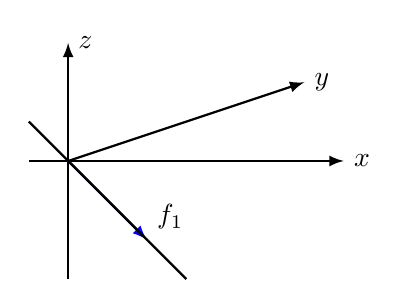
\begin{tikzpicture}[scale=0.5]
	\draw[-latex, thick] (-1,0) -- (7,0)node[right]{$x$};
	\draw[-latex, thick] (0,-3) -- (0,3)node[right]{$z$};
	\draw[-latex, thick] (0,0) -- (6,2)node[right]{$y$};
	\draw[-latex, thick, blue] (0,0) -- (2,-2)node[above right, black]{$f_1$};
	\draw[thick] (-1,1) -- (3,-3);
\end{tikzpicture}}


Отже, розв’язком системи є множина векторів, колінеарних до $f_1$, тобто ядру
лінійного оператора будуть належати вектори простору $E^1$. Базисом ядра є вектор $f_1$.

\subsection{Неоднорідні системи лінійних рівнянь}

Неоднорідна система з $m$ рівнянь та $n$ невідомими має такий вигляд:

$$\begin{matrix}
	a_{11} x_1 + a_{12} x_2 + ... + a_{1n} x_n = b_1, \\
	a_{21} x_1 + a_{22} x_2 + ... + a_{2n} x_n = b_2, \\
	\vdots \\
	a_{m1} x_1 + a_{m2} x_2 + ... + a_{mn} x_n = b_m, \\
\end{matrix}$$


Матриця $A = \begin{pmatrix}
	a_{11} & ...    & a_{1n} \\
	\vdots & \ddots & \vdots \\
	a_{m1} & ...    & a_{mn} \\
\end{pmatrix} = (\overline{a}_1, \overline{a}_2, ..., \overline{a}_n)$ називається основною
матрицею системи, а матриця $\tilde{A} = \begin{pmatrix}
	a_{11} & ...    & a_{1n} & b_1    \\
	\vdots & \ddots & \vdots & \vdots \\
	a_{m1} & ...    & a_{mn} & b_m    \\
\end{pmatrix} = (\overline{a}_1, \overline{a}_2, ..., \overline{a}_n, \overline{b})$ ---
розширеною матрицею системи. В цих означеннях були використані позначення:

$$\overline{a}_i = \begin{pmatrix}
	a_{1i} \\
	a_{2i} \\
	\vdots \\
	a_{mi} \\
\end{pmatrix}, \overline{b} = \begin{pmatrix}
	b_{1} \\
	b_{2} \\
	\vdots \\
	b_{m} \\
\end{pmatrix} \neq \overline{0}.$$


На відміну від однорідної системи, яка завжди має нульовий розв’язок,
неоднорідна система не завжди є сумісною.


Теорема Кронекера-Капеллі. Неоднорідна система лінійних рівнянь є
сумісною тоді і тільки тоді, коли ранги основної та розширеної матриці
співпадають: $\rang A = \rang \tilde{A}$.

Необхідність. Припустимо, що неоднорідна система лінійних рівнянь є
сумісною. Цю систему можна переписати таким чином: 

$$x_1 \begin{pmatrix}
	a_{11} \\
	a_{21} \\
	\vdots \\
	a_{m1} \\
\end{pmatrix} + x_2 \begin{pmatrix}
	a_{12} \\
	a_{22} \\
	\vdots \\
	a_{m2} \\
\end{pmatrix} + ... + x_n \begin{pmatrix}
	a_{1n} \\
	a_{2n} \\
	\vdots \\
	a_{mn} \\
\end{pmatrix} = \begin{pmatrix}
	b_{1} \\
	b_{2} \\
	\vdots \\
	b_{m} \\
\end{pmatrix}$$

або

$$x_1 \overline{a}_1 + x_2 \overline{a}_2 + ... + x_n \overline{a}_n = \overline{b}.$$

Нехай $\rang A = k$ і саме перші $k$ векторів $\overline{a}_1$, $\overline{a}_2$, ..., $\overline{a}_k$ ---
це максимальна лінійно незалежна підсистема векторів-стовпчиків матриці $A$. Це означає, що
елементи $\overline{a}_{k+1}$, $\overline{a}_{k+2}$, ..., $\overline{a}_{n}$ лінійно виражаються через 
$\overline{a}_1$, $\overline{a}_2$, ..., $\overline{a}_k$. Оскільки
система є сумісною, то вона має розв’язки $\alpha_1$, $\alpha_2$, ..., $\alpha_n$ -- це деякий її розв’язок.
Тоді $\alpha_1 \overline{a}_1 + \alpha_2 \overline{a}_2 + ... + \alpha_n \overline{a}_n = \overline{b}$,
тобто вектор $\overline{b}$ лінійно виражається через $\overline{a}_1$, $\overline{a}_2$, ..., $\overline{a}_k$.
А це і означає, що $\rang A = \rang \tilde{A} = k$.

Достатність. Припустимо, що $\rang A = \rang \tilde{A} = k$. Тобто існують константи
$\beta_1$, $\beta_2$, ..., $\beta_k$ такі, що

$$\overline{b} = \beta_1 \overline{a}_1 + \beta_2 \overline{a}_2 + ... + \beta_k \overline{a}_k
 = \beta_1 \overline{a}_1 + \beta_2 \overline{a}_2 + ... + \beta_k \overline{a}_k + 0 \overline{a}_{k+1} + ... + 0 \overline{a}_{n},$$

тобто $\beta_1$, $\beta_2$, ..., $\beta_k$, 0, ..., 0 є розв’язком неоднорідної системи лінійних рівнянь.
Отже, дана система є сумісною.


\textit{Зв’язок між розв’язками однорідної та неоднорідної систем}


Якщо в неоднорідній системі лінійних рівнянь замінити вільні члени нулями,
то отримаємо однорідну систему, яка називається спряженою системою для
відповідної неоднорідної. Між розв’язками цих систем існує зв’язок, який випливає
із наступного твердження.


Тв. Розв’язком неоднорідної системи є сума загального розв’язку відповідної
однорідної (спряженої) системи та деякого часткового розв’язку неоднорідної
системи. 


Доведення. Нехай $\overline{c} = \begin{pmatrix}
	c_1 \\
	\vdots \\
	c_n \\
\end{pmatrix}$ -- це деякий частковий розв’язок неоднорідної
системи, тобто $A \overline{c} = \overline{b}$, а $\overline{f} = \begin{pmatrix}
	f_1 \\
	\vdots \\
	f_n \\
\end{pmatrix}$ -- це загальний розв’язок відповідної однорідної
системи, тобто $A \overline{f} = \overline{0}$. Тоді $A \overline{c} + A \overline{f} = A(\overline{c} + \overline{f}) = \overline{b}$,
а це і означає, що $\overline{c} + \overline{f}$ є
розв’язком системи $A \overline{x} = \overline{b}$.


Висновок. Загальний розв’язок неоднорідної системи можна отримати, якщо
до будь-якого часткового розв’язку цієї системи додати загальний розв’язок
відповідної однорідної (спряженої) системи.


\textit{Алгоритм знаходження розв’язків неоднорідної системи лінійних рівнянь}


Розглянемо неоднорідну систему з $m$ лінійних рівнянь з $n$ невідомими.

1. Записуємо основну матрицю $A$ системи та розширену матрицю $\tilde{A}$.

2. Знаходимо $\rang A$ та $\rang \tilde{A}$ методом обвідних мінорів.

3. Перевіряємо рівність рангів: $\rang A = \rang \tilde{A}$.

4. Якщо $\rang A < \rang \tilde{A}$, то система є несумісною.

5. Якщо ж $\rang A = \rang \tilde{A} = k$, то викреслюємо $(m - k)$ рівнянь, коефіцієнти яких
не входять в базовий мінор.

6. У праву частину переносимо $(n - k)$ невідомих (параметрів), коефіцієнти при
яких не входять в базовий мінор.

7. Розв’язуємо отриману систему і записуємо загальний розв’язок.

8. Виконуємо подвійну перевірку згідно зі структурою розв’язків неоднорідної
системи.


Задача. Знайти загальний розв’язок системи:

$$\begin{matrix}
	x + 2y + 3z = -4, \\
	2x + 3y + 4z = 1, \\
	3x + 4y + 5z = 6. \\
\end{matrix}$$

Розв’язання. Запишемо основну та розширену матриці:

$$A = \begin{pmatrix}
	1 & 2 & 3 \\
	2 & 3 & 4 \\
	3 & 4 & 5 \\
\end{pmatrix}, \tilde{A} = \begin{pmatrix}
	1 & 2 & 3 & -4 \\
	2 & 3 & 4 & 1 \\
	3 & 4 & 5 & 6 \\
\end{pmatrix}.$$

Знайдемо їх ранги методом обвідних мінорів:

$$M_1 = |1| \neq 0 \Rightarrow \rang A \geqslant 1;$$

$$M_2 = \left| \begin{matrix}
	1 & 2 \\
	2 & 3 \\
\end{matrix} \right| = 3 - 4 = -1 \neq 0 \Rightarrow \rang A \geqslant 2;$$

$$M_3^{(1)} = \left| \begin{matrix}
	1 & 2 & 3 \\
	2 & 3 & 4 \\
	3 & 4 & 5 \\
\end{matrix} \right| = \left| \begin{matrix}
	1 &  0 &  0 \\
	2 & -1 & -2 \\
	3 & -2 & -4 \\
\end{matrix} \right| = 0 \Rightarrow \rang A = 2;$$

$$M_3^{(2)} = \left| \begin{matrix}
	1 & 2 & -4 \\
	2 & 3 & 1 \\
	3 & 4 & 6 \\
\end{matrix} \right| = \left| \begin{matrix}
	1 &  0 &  0 \\
	2 & -1 &  9 \\
	3 & -2 & 18 \\
\end{matrix} \right| = 0 \Rightarrow \rang \tilde{A} = 2;$$


отже $\rang A = \rang \tilde{A} = 2$ і система є сумісною. Виберемо два рівняння, які
відповідають базовому мінору $M_2$, $z$ -- параметр:

$$\begin{matrix}
	x + 2y = -4 -3z, \\
	2x + 3y = 1 -4z. \\
\end{matrix}$$

Позначивши $\Delta = M_2 = -1$ і скориставшись формулами Крамера, маємо

$$\Delta_x = \left| \begin{matrix}
	-4 -3z & 2 \\
	 1 -4z & 3 \\
\end{matrix} \right| = -14 -z, x = \dfrac{\Delta_x}{\Delta} = 14 + z,$$

$$\Delta_y = \left| \begin{matrix}
	1 & -4 -3z \\
	2 &  1 -4z \\
\end{matrix} \right| = 9 + 2z, y = \dfrac{\Delta_y}{\Delta} = -9 -2z.$$

Загальний розв’язок має вигляд:

$$\begin{pmatrix}
	x \\
	y \\
	z \\
\end{pmatrix} = \begin{pmatrix}
	14 + z \\
	-9 - 2z \\
	z \\
\end{pmatrix} = \begin{pmatrix}
	14 \\
	-9 \\
	 0 \\
\end{pmatrix} + z \begin{pmatrix}
	 1 \\
	-2 \\
	 1 \\
\end{pmatrix}.$$

Перевірка полягає в тому, що треба переконатися, що стовпчик $\begin{pmatrix}
	14 \\
	-9 \\
	 0 \\
\end{pmatrix}$ є
частковим розв’яз\-ком данної системи, а стовпчик $\begin{pmatrix}
	 1 \\
	-2 \\
	 1 \\
\end{pmatrix}$ -- розв’язком спряженої
системи. 


\section{Лінійні оператори}


\subsection{Лінійний простір лінійних операторів}

Нехай $L$ та $M$ -- лінійні простори над полем $K$. Розглянемо множину лінійних
операторів, які діють з $L$ у $M$. Введемо дві лінійні операції на цій множині.


Озн. Оператор $A$ дорівнює оператору $B$ ($A = B$), якщо для довільного $x \in L$
має місце рівність $A x = B x$.


Озн. Оператор $C$ називається сумою операторів $A$ і $B$ ($C = A + B$), якщо для
довільного $x \in L$ виконується $C x = (A + B)x = A x + B x$.


Тв. 1. Якщо $A$ і $B$ -- лінійні оператори, то оператор $C = A + B$ також є
лінійним.

Доведення. Для будь-яких $x, x' \in L$ виконується співвідношення:

$$C(\alpha x + \beta x') = A(\alpha x + \beta x') + b(\alpha x + \beta x') = \alpha A x + \beta A x' + \alpha B x + \beta B x' =$$

$$= \alpha(A x + B x) + \beta(A x' + B x') = \alpha C x + \beta C x'.$$


Тв. 2. Операція додавання операторів є комутативною та асоціативною, тобто
$A + B = B + A$ та $(A + B) + C = A + (B + C).$

Доведення комутативності. Для довільного $x \in L$ маємо:

$$(A + B)x = A x + B x = B x + A x = (B + A) x.$$


Асоціативність додавання доводиться аналогічно.

Оператори відносно операції додавання утворюють абелеву групу. Нулем
групи (нейтральним елементом) є нульовий оператор: $Ox = \overline{0}$.


Якщо у просторі $L$ зафіксувати базис $e = \{e_1, e_2, ..., e_n\}$, а у просторі $M$ ---
базис $f = \{f_1, f_2, ..., f_n\}$ і побудувати матриці $A_{ef}$ та $B_{ef}$ операторів $A$ та $B$ у
цих базисах, то матриця оператора $C = A + B$ обчислюється за формулою
$C_{ef} = A_{ef} + B_{ef}$.


Озн. Оператор $C$ називається добутком оператора $A$ на константу $\lambda \in K$
($C = \lambda A$), якщо для будь-якого $x \in L$ виконується співввідношення $C x = \lambda A x$.


Тв. 3. Якщо $A$ -- лінійний оператор, то оператор $C = \lambda A$ також є лінійним.

Доведення. Для довільних $x, x' \in L$ виконується співвідношення:

$$C(\alpha x + \beta x') = \lambda A(\alpha x + \beta x') = \lambda \alpha A x + \lambda \beta A x'
= \alpha (\lambda A x) + \beta(\lambda A x') = \alpha C x + \beta C x'.$$

Матриця оператора $C = \lambda A$ обчислюється за формулою $C_{ef} = \lambda A_{ef}$.

Неважко переконатися, що для операцій додавання та множення на константу
виконуються всі властивості, які визначають лінійний простір.


Тв. 4. Множина всіх лінійних операторів, які діють з $L$ у $M$ є лінійним
простором.


\textit{Множення операторів}


Нехай оператори $A$ і $B$ діють таким чином: $B: L \rightarrow M$, $A: M \rightarrow N$, де
$L$, $M$, $N$ -- це деякі лінійні простори.


Озн. Добутком операторів $A$ і $B$ називається оператор $C$ ($C = A B$), якщо
для довільного $x \in L$ виконується $C x = (AB)x = A(B x)$.


Оператор $C = A B$ діє з простору $L$ у простір $N$. Якщо у просторі $L$ та $M$
зафіксовано раніше вибрані базиси, а в просторі $N$ – базис $g = \{g_1, g_2, ..., g_k\}$ і
побудовано матриці $A_{fg}$, $B_{ef}$, то $C_{eg} = A_{fg} B_{ef}$. 

\subsection{Невироджений оператор}

Розглянемо оператор $A: L \rightarrow L$. 


Озн. Оператор $A$ називається невиродженим, якщо його ядро містить лише
нульовий елемент, тобто $\Ker A = \{\overline{0}\}$. В іншому випадку оператор $A$ називається
виродженим.


Приклади.

1. Тотожній оператор $I x = x$ є невиродженим.

2. Розглянемо оператор $P: E^2 \rightarrow E^2$, який проектує довільний вектор з $E^2$ на
вісь абсцис. Цей оператор є виродженим.


Озн. Рангом лінійного оператора називається розмірність його образу, тобто
$\rang A = \dim \im A$.


Тв. 1. Якщо оператор $A$ є невиродженим, то $\rang A = \dim L$.

Доведення. Твердження випливає з теореми про розмірності ядра і образу
лінійного оператора (див. властивості лінійних операторів):

$$\dim L = \dim \Ker A + \dim \im A$$

(враховується, що $\dim \Ker A = 0$).



Тв. 2. Якщо оператори $A$ і $B$ є невиродженими, то оператор $C = A B$ є також
невиродженим.

Доведення. Нехай $x \in \Ker C$. Тоді $C x = (A B)x = \overline{0}$. Звідси випливає, що
$(AB)x = A(Bx) = \overline{0}$. З означення невиродженості оператора $A$ випливає, що
$B x = 0$, а з невиродженості оператора $B$ слідує, що $x = \overline{0}$. Це і означає, що
$\Ker C = \{\overline{0}\}$, тобто оператор $C = A B$ є невиродженим.


Тв. 3. Якщо оператор $A$ є невиродженим і $A x = y$, то для елементу $y$ існує
єдиний прообраз $x$.

Доведення проведем від супротивного. Припустимо, що $A x = y$, $A x' = y$ і
$x \neq x'$. Тоді $Ax - Ax' = A(x - x') = 0$, тобто $x - x' \in \Ker A$. Тому $x - x' = \overline{0}$ і
$x = x'$, що суперечить припущенню.

Дане твердження дає змогу ввести поняття оберненого оператора. 

Озн. Нехай $A x = y$ і оператор $A$ є невиродженим. Оператор $A^{-1}$, що
задовольняє співвідношення $A^{-1} y = x$ називається оберненим до $A$.

Тв. 4. $A^{-1}A = A A^{-1} = I$.

Доведення. Це твердження випливає із співвідношень:

$$A^{-1}(Ax) = A^{-1}y = x \text{ або } (A^{-1}A)x = Ix.$$

Отже, $A^{-1}A = I$, де $I$ -- це тотожній оператор ($Ix = x$). Аналогічно доводиться, що
$AA^{-1} = I$.


Тв 5. Якщо невироджений оператор $A$ є лінійним, то і оператор $A^{-1}$ -- лінійний.


Доведення. Позначимо $z = A^{-1}(\alpha y + \beta y') - \alpha A^{-1} y - \beta A^{-1} y'$. Подіємо на
обидві частини цієї рівності оператором $A$:

$$Az = AA^{-1}(\alpha y + \beta y') - \alpha A A^{-1} y - \beta A A^{-1} y' = \alpha y + \beta y' - \alpha y - \beta y' = \overline{0}.$$

Звідси випливає, що $z \in \Ker A$. Але $A$ -- невироджений оператор, тому $z = \overline{0}$.

Тобто $A^{-1}(\alpha y + \beta y') = \alpha A^{-1} y + \beta A^{-1} y'$ -- це і означає лінійність оператора $A^{-1}$.


Тв 6. Оператор $A^{-1}$ є невиродженим.

Доведення. Для довільного $y \in \Ker A^{-1}$ маємо $A^{-1} y = \overline{0}$. На обидві частини
цієї рівності подіємо оператором $A$. Тоді $A A^{-1} y = A \overline{0} = \overline{0}$. Оскільки
$A A^{-1} = I$, то $y = \overline{0}$, що і доводить невиродженість оператора $A^{-1}$.


Якщо лінійному оператору $A$ відповідає в деякому базисі матриця $A'$, то
оберненому лінійному оператору $A^{-1}$ відповідатиме матриця $A'^{-1}$.


Умова невиродженості оператора $A$ еквівалентна умові існування $A'^{-1}$.

Дійсно, для знаходження ядра $A$ треба розв’язати систему $A'\overline{x} = \overline{0}$. Однорідна
система лінійних рівнянь завжди має нульовий розв’язок. Цей розв’язок буде
єдиним тоді і тільки тоді, коли $\rang A' = n$ ($n$ -- кількість невідомих, $n = \dim L$).

Оскільки матриця $A'$ має розмірність $n \times n$, то $\rang A' = n \Leftrightarrow \det A' \neq 0 \Leftrightarrow \exists A'^{-1}$.


\section{Аналітична геометрія у просторі}


%\subsection{Площина у просторі}
%\subsection{Пряма у просторі}
%\subsection{Поверхні другого порядку}


\subsection{Площина у просторі}

Нехай у просторі задана площина $P$, точка $M_0(x_0,y_0,z_0)$ та
$n = (A,B,C) \neq 0$, $\overline{n} \perp P$.

Озн. Вектор $n \perp P$ називається нормальним вектором площини,
задається він єдиним чином з точністю до ненульової константи.







Нехай т. $M(x,y,z)$ -- довільна точка простору.
$\overline{M_0 M} = (x-x_0,y-y_0,z-z_0)$.

Тв. $M \in P \Leftrightarrow \overline{n} \perp \overline{M_0 M} \Rightarrow (\overline{n},\overline{M_0 M}) = 0$


$$A(x - x_0) + b(y - y_0) + C(z - z_0) = 0.$$

Отримали рівняння площини $P$, яка задана
точкою та нормальним вектором. Розкриваючи
дужки, маємо:

$$Ax + By + Cz - Ax_0 - By_0 - Cz_0 = 0;$$

$Ax + By + Cz + D = 0$ -- загальне рівняння
площини.


\subsection{Неповні рівняння площини}

Виходячи з геометричного тлумачення коефіцієнтів $A$, $B$, і $C$ як
координат вектора її нормалі, дослідимо питання про їх вплив на розміщення
площини відносно системи координат.

$P: Ax + Bx + Cz + D = 0$; $M_0(x_0,y_0,z_0) \in P$;

1) $\overline{n} = (0,0,C) \parallel (0,0,1)$, $n \perp XOY$,
$P : z - z_0 = 0 \Rightarrow z = z_0$ -- площина $\perp XOY$.

Частковий випадок: $z = 0$ -- сама площина $XOY$.

2) $\overline{n} = (0,B,0) \parallel (0,1,0)$; $P: y = y_0 \parallel XOZ$.

3) $\overline{n} = (A,0,0) \parallel (1,0,0)$; $P: x = x_0 \parallel YOZ$.

4) $ABCD \neq 0 \Rightarrow (0,0,0) \notin P$ і $P$ не паралельна жодній координатній
площині. Така площина називається площиною загального розташування.


\subsection{Рівняння площини «у відрізках»}

Нехай $P: Ax + By + Cz + D = 0$; $ABCD \neq 0 \Rightarrow$

$$\dfrac{x}{\dfrac{D}{A}} + \dfrac{y}{\dfrac{D}{B}} + \dfrac{z}{\dfrac{D}{C}} = 1;
\dfrac{x}{a} + \dfrac{y}{b} + \dfrac{z}{c} = 1
\text{ -- рівняння площини у відрізках}.$$


Зауважимо, що числа $a$, $b$, $c$ мають простий геометричний зміст: вони
дорівнюють величинам відрізків, які відтинає площина на осях $Ox$, $Oy$, і
$Oz$ (з урахуванням знаків).

Справді, якщо дану площину $P$
перетнути площинами $y = 0$ і $z = 0$,
маємо, що точка $M_1(a,0,0) \in P$.
Аналогічно $M_2(0,b,0) \in P$,
$M_3(0,0,c) \in P$.


\subsection{Нормальне рівняння площини}

Нехай площина $P$, що не
проходить через $O(0,0,0)$, задана так:
її нормальний вектор $\overline{n}$ проведено з
початку координат в напрямку
площини; $|\overline{n}| = p > 0$; його кути з
координатними осями -- ($\alpha$, $\beta$, $\gamma$).

$$\overline{n}_0 = \dfrac{1}{|\overline{n}|}\overline{n}; \overline{n}_0 = {\cos \alpha, \cos \beta, \cos\gamma};$$

$$|\overline{n}_0| = 1.$$

Точка $M(x,y,z)$ -- довільна; $\overline{OM} = (x, y,z)$.

Зрозуміло, що $M \in P \Leftrightarrow \text{np}_{\overline{n}}\overline{OM} = p$; $\text{np}_{\overline{n}}\overline{OM} = \text{np}_{\overline{n}_0} \overline{OM}(\overline{n}_0, \overline{OM}) = p$ або
$x \cos \alpha + y \cos \beta + z \cos \gamma = p$;

$x \cos \alpha + y \cos \beta + z \cos \gamma - p = 0$ -- нормальне рівняння площини.

Щоб звести рівняння $Ax + By + Cz + D$ до нормального, треба праву і
ліву частину помножити на $M = \dfrac{- \text{sigh} D }{\sqrt{A^2 + B^2 + C^2}}$.

Приклад. Звести рівняння площини $P: 2x - 3y + 6z + 14 = 0$ до нормального
виду.

Розв’язання. Нормуючим множником для даного рівняння буде
$M = \dfrac{- 1 }{\sqrt{2^2 + 3^2 + 6^2}} = -\dfrac{1}{7}$. Знак числа $M$ завжди протилежний знаку вільного
члена D.

$$P: -\dfrac{1}{7}(2x - 3y + 6z + 14) = 0; p = 2.$$


\subsection{Відхилення і відстань від точки до площини}

Нехай задано площину $P: Ax + By + Cz + D = 0$; $D \neq 0$ і точку
$M_0(x_0,y_0,z_0) \notin P$.

$P: x \cos \alpha + y \cos \beta + z cos \gamma - p = 0$.

І нехай $\rho(M_0,P) = d > 0$ -- відстань від $M_0$ до $P$.

Озн. Відхиленням $M_0$ від $P$ (позначається $\delta_{M_0P}$) називається величина

$\delta_{M_0P} = \left\{\begin{matrix}
	d \text{, якщо} M_0 \text{ і } O(0,0,0)\text{ лежать по різні боки від } P, \\
	-d \text{, якщо} M_0 \text{ і } O(0,0,0)\text{ лежать по одну сторону від } P. \\
\end{matrix} \right.$



Побудуємо $P' \parallel P$, $M_0 \in  P'$.

$P': x \cos \alpha + y \cos \beta + z \cos \gamma - (p + \delta_{M_0P}) = 0$.

Враховуючи, що $M_0 \in P$, маємо:

$$x_0 \cos \alpha + y_0 \cos \beta + z_0 \cos \gamma - p - \delta_{M_0P} = 0 \Rightarrow$$.

$$\delta_{M_0P} = x_0 \cos \alpha + y_0 \cos \beta + z_0 \cos \gamma - p;$$

$$d = \rho(M_0,P) = |\delta_{M_0P}| = |x_0 \cos \alpha + y_0 \cos \beta + z_0 \cos \gamma - p|.$$



\subsection{Взаємне розташування площин}

$$P_1: A_1 x + B_1 y + C_1 z + D_1 = 0, \overline{n}_1 = (A_1,B_1,C_1), M_1(x_1,y_1,z_1)\in P_1.$$

$$P_2: A_2 x + B_2 y + C_2 z + D_2 = 0, \overline{n}_2 = (A_2,B_2,C_2), M_2(x_2,y_2,z_2)\in P_2.$$

1) Площини $P_1$ і $P_2$ співпадають; $P_1 = P_2$.

Тоді $\rang \begin{pmatrix}
	A_1 & B_1 & C_1 & D_1 \\
	A_2 & B_2 & C_2 & D_2 \\
\end{pmatrix} = 1.$

2) $P_1 \neq P_2$, $P_1 \parallel P_2$.

Тоді $\overline{n}_1 \parallel \overline{n}_2$ і $\rang \begin{pmatrix}
	A_1 & B_1 & C_1 \\
	A_2 & B_2 & C_2 \\
\end{pmatrix} = 1$, а $\rang \begin{pmatrix}
	A_1 & B_1 & C_1 & D_1 \\
	A_2 & B_2 & C_2 & D_2 \\
\end{pmatrix} = 2$.

Відстань від $P_1$ до $P_2$ -- $\rho(P_1,P_2)$ доцільно шукати, як відстань від $M_2$ до $P_1$:

$$\rho(P_1,P_2) = \rho(M_2,P_1) = \dfrac{|A_1 x_2 + B_1 y_2 + D_1 z_2 + D_1|}{\sqrt{A_1^2 + B_1^2 + C_1^2}}.$$


3) $P1 \nparallel P_2$;

$$\overline{n}_1 \nparallel \overline{n}_2 \Leftrightarrow \rang \begin{pmatrix}
	A_1 & B_1 & C_1 \\
	A_2 & B_2 & C_2 \\
\end{pmatrix} = 2.$$


Якщо $\alpha = (\widehat{P_1,P_2})$, то $\cos \alpha = |\cos(\widehat{\overline{n}_1,\overline{n}_2})|
= \dfrac{|A_1A_1 + B_1B_1 + C_1C_1|}{\sqrt{A_1^2 + B_1^2 + C_1^2}\sqrt{A_2^2 + B_2^2 + C_2^2}}$.


\subsection{Пряма у просторі}


Пряма у просторі задається двома принципово різними способами.

I спосіб. Нехай $l$ -- пряма, точка $M_0(x_0,y_0,z_0) \in l$,


Озн. Вектор $\overline{q} = (a,b,c) \neq 0$, $\overline{q} \parallel l$ називається напрямним вектором
прямої $l$.

Точка $M(x,y,z)$ -- довільна точка простору.


$\overline{M_0M} = (x-x_0,y-y_0,z-z_0)$.
Зрозуміло, що $M \in L \Leftrightarrow \overline{M_0M} \parallel q$ або

$$\dfrac{x-x_0}{a} = \dfrac{y-y_0}{b} = \dfrac{z-z_0}{c}.(1)$$

Ми отримали так зване канонічне
рівняння прямої.


Рівняння $\dfrac{x-x_0}{a} = \dfrac{y-y_0}{b}$, $\dfrac{x-x_0}{a} = \dfrac{z-z_0}{c}$
і $\dfrac{y-y_0}{b} = \dfrac{z-z_0}{c}$ -- рівняння
площин, що проектують пряму $l$ на координатні площини.

II спосіб. Площини $P_1$ і $P_2$, $P_1 \nparallel P_2$ задаються рівняннями:

$$P1: A_1x + B_1y + C_1z + D_1 = 0.$$
$$P2: A_2x + B_2y + C_2z + D_2 = 0.$$

Пряму $l$ задають як перетин $P_1$ і $P_2$:

$$l: \left\{ \begin{matrix}
	A_1x + B_1y + C_1z + D_1 = 0
	A_2x + B_2y + C_2z + D_2 = 0
\end{matrix} \right. (2)$$


Для того, щоби звести рівняння прямої типу (2) до вигляду (1), треба
знайти напрямний вектор $\overline{q}$ і якусь точку $M_0(x_0,y_0,z_0)$, що належить $l$.

$\overline{q} \perp \overline{n}_1(A_1,B_1,C_1)$, $\overline{q} \perp \overline{n}_2 = (A_2,B_2,C_2) \Rightarrow \overline{q} = [\overline{n}_1,\overline{n}_2].$


Якщо систему (2) розглядати як неоднорідну систему лінійних рівнянь
(за умовою вона сумісна!), то якийсь її частковий розв’язок $(x_0,y_0,z_0)$ дасть
нам координати точки $M_0$.

Як наслідок рівняння прямої типу (1) є її параметричне рівняння:

$$\dfrac{x-x_0}{a} = \dfrac{y-y_0}{b} = \dfrac{z-z_0}{c} = t, t \in (-\infty;+\infty) \Rightarrow 
\left\{ \begin{matrix}
	x = at +x_0; \\
	y = bt +y_0; \\
	z = ct +z_0. \\
\end{matrix} \right.$$


\subsection{Взаємне розташування прямої і площини}


Нехай дано:
пряма $l: \dfrac{x-x_0}{a} = \dfrac{y-y_0}{b} = \dfrac{z-z_0}{c}$, $\overline{q} = (a,b,c)$,
$M_0(x_0,y_0,z_0)$,
площина $P: Ax + By + Cz + D = 0$, $\overline{n} = (A,B,C)$.

1. $l \subset P$ -- пряма лежить в площині. 
$n \perp q$,
$M_0 \in P$, $(\overline{n},\overline{q}) = 0 \Rightarrow Aa + Bb + Cc = 0$.


2. $l \parallel P$ -- пряма паралельна площині.

$\overline{q} \perp \overline{n}$, $M_0 \notin P$.

Відстань між прямою і площиною
$\rho(l,P) = \rho(M_0,P)$ і
знаходиться стандартним методом.


3. $l \nparallel P$, $l \cap P = \{K\}$ — пряма перетинає площину в точці K.

Вектори $\overline{n}$ та $\overline{q}$ -- не перпендикулярні
$\Rightarrow (\overline{n},\overline{q}) \neq 0 \Rightarrow Aa + Bb + Cc \neq 0$.

Зауваження. Щоб знайти координати точки $K$, доцільно
використовувати параметричне рівняння прямої.

Частковий випадок:
$l \perp P \Rightarrow \overline{q} \parallel \overline{n}$.


\subsection{Взаємне розташування двох прямих}

$$l_1: \dfrac{x-x'_0}{a_1} = \dfrac{y-y'_0}{b_1} = \dfrac{z-z'_0}{c_1},
\overline{q}_1 = (a_1,b_1,c_1),
M_1(x'_0,y'_0,z'_0) \in l_1;$$

$$l_2: \dfrac{x-x''_0}{a_2} = \dfrac{y-y''_0}{b_2} = \dfrac{z-z''_0}{c_2},
\overline{q}_2 = (a_2,b_2,c_2),
M_2(x''_0,y''_0,z''_0) \in l_2.$$

1. $l_1 \parallel l_2$, ($l_1 \neq l_2$) -- прямі не співпадають і паралельні.


У цьому випадку $\overline{q}_1 \parallel \overline{q}_2$, а $M_1 \notin l_2$.

Відстань між паралельними прямими
простіше за все шукати, як висоту
паралелограма, побудованого на
векторах $\overline{q}_1$ і $\overline{M_1M_2}$:

$$\rho(l_1,l_2) = h = \dfrac{|[\overline{q}_1,\overline{M_1,M_2}]|}{|\overline{q}_1|}.$$



2. $l_1 \cap l_2 = \{K\}$ -- прямі перетинаються в точці $K$.


У цьому випадку вектори $q_1$, $q_2$ і
$\overline{M_1M_2}$ -- компланарні,
тобто $\overline{q}_1 \overline{q}_2 \overline{M_1M_2} = 0 \Rightarrow$

$$\Rightarrow \left| \begin{matrix}
	a_1 & b_1 & c_1 \\
	a_2 & b_2 & c_2 \\
	x'_0 - x''_0 & y'_0 - y''_0 & z'_0 - z''_0 \\
\end{matrix} \right| = 0.$$



3. $l_1 \nparallel l_2$, $l_1 \cap l_2 = \varnothing$ -- прямі мимобіжні.


У такому випадку прямі не
паралельні і не лежать в одній
площині $\Rightarrow$

$V = |\overline{q}_1 \overline{q}_2 \overline{M_1M_2}| \neq 0$, де $V$ -- об’єм
паралелепіпеда, побудованого на цих
трьох векторах.

Довести, що відстань між прямими

$$\rho(l_1,l) = \dfrac{|\overline{q}_1 \overline{q}_2 \overline{M_1M_2}|}{|[\overline{q}_1,\overline{q}_2]|}$$


Спільний перпендикуляр $L$ до прямих $l_1$ і $l_2$ пропонується знаходити за
такою схемою:

а) Знайти нормальні вектори площин $P_1$ і $P_2$, де $P_1 \supset l_1$, $P_1 \parallel l_2 \Rightarrow$

$\Rightarrow \overline{n}_1 \perp \overline{q}_1$, $\overline{n}_1 \perp \overline{q}_2 \Rightarrow \overline{n}_1 = [\overline{q}_1,\overline{q}_2]$, $\overline{n}_2 = \overline{n}_1$.

б). Знайти рівняння площин $P_3$ і $P_4$:

$$P_3 \supset l_1, P_3 \perp P_1 \Rightarrow \overline{n}_3 = [\overline{q}_1,\overline{n}_1], M_1 \in P_3,$$

$$P_4 \supset l_2, P_4 \perp P_1 \Rightarrow \overline{n}_4 = [\overline{q}_2,\overline{n}_1], M_2 \in P_4.$$


в). $L: \left\{ \begin{matrix}
	P_3 \\
	P_4 \\
\end{matrix} \right. .$


\subsection{Поверхні другого порядку}

Загальний вид поверхні другого порядку:

$$Ax^2 + By^2 + Cz^2 + Dxy + Fxz + Eyz + Ix + Gy + Kz + L = 0.$$

При різних значеннях коефіцієнтів це можуть бути власне поверхні,
площини, прямі, точки, уявні поверхні. Ми ж будемо розглядати канонічні
рівняння поверхонь другого порядку. Основний метод їх дослідження ---
метод перетину.


\subsection{Еліпсоїд}

$$\dfrac{x^2}{a^2} + \dfrac{y^2}{b^2} + \dfrac{z^2}{c^2} = 1 (\text{Тут і далі } a  > 0, b > 0 , c > 0).$$

$$\dfrac{x^2}{a^2} = 1 - \dfrac{y^2}{b^2} - \dfrac{z^2}{c^2} \leqslant 1 \Rightarrow |x| \leqslant a.$$


а це означає, що вся наша поверхня лежить між площинами $x = - a$ і
$x = a$. З аналогічних міркувань вона розташована між $y = -b$, $y = b$ та $z = -c$,
$z = c$. Перетнемо цю поверхню площиною $z = C$, $|C| \leqslant c$.

$$\dfrac{x^2}{a^2} + \dfrac{y^2}{b^2} = 1 - \dfrac{C^2}{c^2}$$ -- проекція перетину на $XOY$.

$\dfrac{x^2}{a^2\left(1-\dfrac{C^2}{c^2}\right)} + \dfrac{y^2}{b^2\left(1-\dfrac{C^2}{c^2}\right)} = 1$ ---
отримали еліпс з півосями $a\sqrt{1 - \dfrac{C^2}{c^2}}$ та $b\sqrt{1 - \dfrac{C^2}{c^2}}$.


Зрозуміло, що з ростом $C$ півосі зменшуються. Якщо $z = 0$, то в
перетині маємо еліпс $\dfrac{x^2}{a^2} + \dfrac{y^2}{b^2} = 1$.


Перетинаючи нашу поверхню двома іншими координатними площинами
$y = 0$ та $z = 0$, маємо ще два еліпси: $\dfrac{x^2}{a^2} + \dfrac{z^2}{c^2} = 1$
і $\dfrac{y^2}{b^2} + \dfrac{z^2}{c^2} = 1$.

Отриманої інформації вистачає,
щоб побудувати поверхню.


\subsection{Гіперболоїд}

а) однопорожнинний

$$\dfrac{x^2}{a^2} + \dfrac{y^2}{b^2} - \dfrac{z^2}{c^2} = 1.$$

Спочатку дещо з’ясуємо про розташування цієї поверхні.

$$\dfrac{x^2}{a^2} + \dfrac{y^2}{b^2} = 1 + \dfrac{z^2}{c^2} \geqslant 1 \Rightarrow \dfrac{x^2}{a^2} + \dfrac{y^2}{b^2} \geqslant 1.$$

Це означає, що всі точки поверхні проектуються поза еліпсом

$$\dfrac{x^2}{a^2} + \dfrac{y^2}{b^2} = 1.$$

Перетнемо поверхню площиною $z = C$. 

$$\dfrac{x^2}{a^2} + \dfrac{y^2}{b^2} = 1 + \dfrac{C^2}{c^2} \Rightarrow 
\dfrac{x^2}{a^2\left(1+\dfrac{C^2}{c^2}\right)} + \dfrac{y^2}{b^2\left(1+\dfrac{C^2}{c^2}\right)} = 1.$$


Тобто, лінії перетину проектуються у еліпси, півосі яких зростають зі
збільшенням $C$.

Якщо поверхню перетнути площинами $x = 0$ і $y = 0$, отримаємо у
вертикальних координатах площинах гіперболи: 

$\dfrac{y^2}{b^2} - \dfrac{x^2}{c^2} = 1$, $\dfrac{x^2}{a^2} - \dfrac{x^2}{c^2} = 1$.


Цієї інформації вистачає, щоб побудувати поверхню.


б) двопорожнинний

$$\dfrac{x^2}{a^2} + \dfrac{y^2}{b^2} - \dfrac{z^2}{c^2} = -1.$$

$$\dfrac{z^2}{c^2} = \dfrac{x^2}{a^2} + \dfrac{y^2}{b^2} + 1 \geqslant 1, \Rightarrow
\dfrac{z^2}{c^2} \geqslant 1 \Rightarrow |z| \geqslant c.$$

Це означає, що вся поверхня лежить вище ніж площина $z = c$ і нижче
ніж площина $z = -c$. В перетині з площинами $z = C$ маємо еліпси, параметри 
яких збільшуються з ростом $|c|$, а в перетині з площинами $y = 0$ і $x = 0$ ---
гіперболи

$\dfrac{x^2}{a^2} - \dfrac{z^2}{c^2} = -1$ та $\dfrac{y^2}{b^2} - \dfrac{z^2}{c^2} = -1$.


\subsection{Параболоїд}

а) еліптичний

$$z = \dfrac{x^2}{a^2} + \dfrac{y^2}{b^2}.$$

Уся поверхня лежить у верхній частині простору, бо $z \geqslant 0$.

У перетині з площинами $z = C \geqslant 0$ маємо еліпси, що збільшуються з
ростом $C$.

А в перетині з координатними площинами $y = 0$ і $x = 0$ -- параболи

$z = \dfrac{x^2}{a^2}$ і $z = \dfrac{y^2}{b^2}$.



б) гіперболічний

$$z = \dfrac{x^2}{a^2} - \dfrac{y^2}{b^2}.$$

У перетині з площиною $y = 0$ маємо параболу $z = \dfrac{x^2}{a^2}$, а з площиною
$x = 0$ -- $z = \dfrac{y^2}{b^2}$. При $z = C > 0$ у перетині маємо гіперболи
$\dfrac{x^2}{a^2 c} - \dfrac{y^2}{b^2 C} = 1$, а при $z = c < 0$ -- спряжені гіперболи
$\dfrac{x^2}{a^2 c} - \dfrac{y^2}{b^2 C} = 1$.


\subsection{Конус другого порядку}

$$\dfrac{x^2}{a^2} + \dfrac{y^2}{b^2} - \dfrac{z^2}{c^2} = 0.$$

Ця поверхня у перетині з площинами $z = C$ утворюють еліпси.

А при $y = 0$ маємо дві прямі:$\dfrac{x^2}{a^2} = \dfrac{z^2}{c^2} \Rightarrow
z = \dfrac{c}{a}x$ і $z = - \dfrac{c}{a}x$

При $x = 0$ -- прямі $z = \pm \dfrac{c}{b}y$

\subsection{Циліндри другого порядку}

а) еліптичний

$$\dfrac{x^2}{a^2} + \dfrac{y^2}{b^2} = 1.$$


б) гіперболічний

$$\dfrac{x^2}{a^2} - \dfrac{y^2}{b^2} = 1.$$


в) параболічний

$$y^2 = 2px$$


\section{Лінійна алгебра}


\subsection{Лінійні простори. Лінійні оператори (продовження)}

\subsection*{Сума та перетин лінійних підпросторів}

Нехай $L$ -- деякий лінійний простір, $L_1$, $L_2$, -- його підпростори.

Озн .Сумою $L_1 + L_2$ лінійних підпросторів $L_1$ і $L_2$ є:
$L_1 + L_2 = \{ x \in L: x = x_1 + x_2, \forall x_1 \in L_1, \forall x_2 \in L_2\}$.


Озн .Перетином $L_1 \cap L_2$ підпросторів $L_1$ і $L_2$ є:
$L_1 \cap L_2 = \{x \in L: x \in L_1 \wedge x \in L_2 \}$.


Твердження. Сума і перетин $L_1$ і $L_2$ є підпросторами $L$.


Доведення. Нехай $x,y \in L_1 + L_2$; $x = x_1 + x_2$, $x_1 \in L_1$, $x_2 \in L_2$,

$y = y_1 + y_2$, $y_1 \in L_1$, $y_2 \in L_2$.

Тоді $\alpha x + \beta y = \alpha(x_1 + x_2) + \beta(y_1 + y_2) = (\alpha x_1 + \beta y_1) + (\alpha x_2 + \beta y_2):$

$\alpha x_1 + \beta y_1 \in L_1$, $\alpha x_2 + \beta y_2 \in L_2 \Rightarrow \alpha x + \beta y \in L_1 + L_2.$

І нехай $x,y \in L_1 \cap L_2$.

Тоді $\alpha x + \beta y \in L_1$, $\alpha x + \beta y \in L_2 \Rightarrow \alpha x + \beta y \in L_1 \cap L_2$.


Приклади.
а)
Рис. 1

$$L_1 = E^1, L_2 = E^1,$$

$$L_1 \cap L_2 = \{\overline{0}\},$$

$$L_1 + L_2 = E^2.$$


б)

$$L_1 = E^2, L_2 = E^1,$$

$$L_1 + L_2 = E^3,$$

$$L_1 \cap L_2 = \{\overline{0}\}.$$


в)

$$L_1 = E^2, L_2 = E^2,$$

$$L_1 + L_2 = E^3,$$

$$L_1 \cap L_2 = E^1.$$



Теорема. $\dim(L_1 + L_2) = \dim L_1 + \dim L_2 - \dim(L_1 \cap L_2)$.

Доведення. Нехай $\dim(L_1 \cap L_2) = k$ і вектори $\{g_1, g_2, ..., g_k\}$ -- базис
$L_1 \cap L_2$. Якщо $\dim L_1 = m$, можемо побудувати такий базис
$L_1: \{f_1, ..., f_{m-k}, g_1, ..., g_k\}$.


Аналогічно: $\dim L_2 = p$, $\{g_1, ..., g_k, t_1, ..., t_{p-k}\}$ -- базис $L_2$.

Розглянемо систему векторів:

$\{f_1, ..., f_{m-k}, g_1, ..., g_k, t_1, ..., t_{p-k}\} (*)$

і доведемо, що вона є базисом $L_1 + L_2$.

$$\forall x \in L_1 + L_2, x = x_1 + x_2
= \left( \sum\limits_{i=1}^{m-k} \alpha_i f_i
		+ \sum\limits_{i=1}^{k} \beta_i g_i \right)
+ \left( \sum\limits_{i=1}^{k} \gamma_i g_i
		+ \sum\limits_{i=1}^{p-k} \delta_i t_i \right) = $$
		
$$= \sum\limits_{i=1}^{m-k} \alpha_i f_i
+ \sum\limits_{i=1}^{k} (\beta_i \gamma_i)g_i
+ \sum\limits_{i=1}^{p-k} \delta_i t_i.$$


Таким чином, система (*) є повною в $L_1 + L_2$. Припустимо, що (*) ---
лінійно залежна, тобто $\exists \alpha_i, \beta_i, \gamma_i$ не всі водночас нульові, такі, що

$$\alpha_1 f_1 + ... + \alpha_{m-k} f_{m-k} + \beta_i g_i + ... + \beta_k g_k + \gamma_i t_i + ... + \gamma_{p-k} t_{p-k} = 0. (1)$$

Позначимо: $y = \gamma_i t_i + ... + \gamma_{p-k} t_{p-k}$. (2)

Зрозуміло, що $y \in L_2$. Але із (1) $\Rightarrow y \in L_1$.

Тобто, $y \in L_1, l_2$. Тоді $y = v_1 g_1 + ... + v_k g_k$. (3)

Із (2) та (3) $\Rightarrow v_1 g_1 + ... + v_k g_k + (-\gamma_1) t_1 + ... + (-\gamma_{p-k}) t_{p-k} = 0 \Rightarrow$

$\Rightarrow \forall v_i = 0 \forall \gamma_i = 0$
через лінійну незалежність $\{g_1, ..., g_k, t_1, ..., t_{p-k}\}$.

Маємо із (1) $\alpha_1 f_1 + ... + \alpha_{m-k} f_{m-k} = 0 \Rightarrow \forall \alpha_i = 0$ з
таких же міркувань.

Таким чином, наше припущення, що у (1) деякі коефіцієнти $\neq 0$ невірне,
що й доводить лінійну незалежність системи (*).

Отримали, що система (*) повна у $L_1 + L_2$ і лінійно незалежна $\Rightarrow$ вона є
базисом у $L_1 + L_2$.


Кількість векторів у системі (*): $(m - k) + k + (p - k) = m + p - k$,
що і доводить теорему. 

\subsection*{Пряма сума лінійних підпросторів}

Нехай $L$ -- лінійний простір, $L_1 \subset L$, $L_2 \subset L$.

Озн. Сума $L_1 + L_2$ називається прямою (позначається $L+1 \dotplus L_2$), якщо
$\forall x \in L_1 + L_2$, $x = x_1 + x_2$, $x_1 \in L_1$, $x_2 \in L_2$ і цей розклад єдиний.

Приклади 1) і 2) є прикладами прямої суми, а 3) -- ні.

Теорема 2. Лінійний простір $L$ розкладається у пряму суму своїх
підпросторів $L = L_1 \dotplus L_2$ тоді і тільки тоді, коли об’єднання базисів
підпросторів є базисом всього $L$.

Доведення. Нехай $L = L_1 \dotplus L_2$, $\{f_1, ..., f_m\}$ -- базис $L_1$, $$\{g_1, ..., g_k\}$$ -- базис
$L_2$.


$$\forall x \in L_1 \dotplus L_2, x = x_1 + x_2, x_1 \in L_1, x_2 \in L_2$$

$$x_1 = \alpha_1 f_1 + ... + \alpha_m f_m, x_2 = \beta_1 g_1 + ... + \beta_k g_k \Rightarrow$$

$$x = \alpha_1 f_1 + ... + \alpha_m f_m + \beta_1 g_1 + ... + \beta_k g_k,$$

тобто система векторів

$\{f_1, ..., f_m, g_1, ..., g_k\} *)$

є повною в $L_1 + L_2$.

Доведемо, що система *) -- лінійно незалежна. Припустимо, що
$\exists \alpha_i \neq 0$ і $\exists \beta_i \neq 0$ є такі, що

$$\alpha_1 f_1 + ... + \alpha_m f_m + \beta_1 g_1 + .. + \beta_k g_k = 0. (1)$$

Вектор 0, який стоїть праворуч, можна представити у вигляді $0 = 0 + 0$ і цей
розклад єдиний.

Із (1) випливає: $\alpha_1 f_1 + ... + \alpha_m f_m = 0$, $\beta_1 g_1 + .. + \beta_k g_k = 0$,
а із лінійної незалежності базисів $L_1$ і $L_2$: $\forall \alpha_i = 0$ і $\forall \beta_i = 0$,
що доводить першу частину теореми.

Тепер припустимо, що система *) -- базис $L_1 + L_2$.

$$\forall x \in L_1 + L_2: x = \alpha_1 f_1 + ... + \alpha_m f_m + \beta_1 g_1 + ... + \beta_k g_k$$

і цей розклад єдиний. Тобто $x = x_1 + x_2$, де $x_1 = \alpha_1 f_1 + ... + \alpha_m f_m \in L_1$,
$x_2 = \beta_1 g_1 + ... + \beta_k g_k \in L_2$. Це і доводить той факт, що сума $L_1 \dotplus L_2$ -- пряма.
Теорему доведено. 

\subsection{Перехід до іншого базису}

\subsection*{Перетворення координат вектора при зміні базису}

Нехай $L$ -- лінійний простір, $\dim L = n$, $\{e_1, ..., e_m\}$ -- базис цього простору,
який ми умовно будемо називати «старим».

Якщо $x \in L$, то: $x = x_1 e_1 + x_2 e_2 + ... + x_n e_n. (1)$

Таким чином, кожному елементу $x \in L$ можна поставити у взаємно
однозначну відповідність стовпчик координат цього вектора за «старим»
базисом:

$$L \ni x \leftrightarrow \overline{x} = \begin{pmatrix}
	x_1 \\
	x_2 \\
	\vdots \\
	x_n \\
\end{pmatrix} \in R^n.$$

Якщо ж взяти в тому ж просторі якийсь інший («новий») базис
$\{f_1, ..., f_n\}$, то той же вектор $x$ можна розкласти за ним і отримати стовпчик
«нових» координат: $x = \tilde{x}_1 f_1 + \tilde{x}_2 f_2 + ... + \tilde{x}_n f_n = \sum\limits_{j=1}^N \tilde{x}_j f_j. (2)$

Тобто, тому ж самому елементу x відповідатиме інший стовпчик:

$$L \ni x \leftrightarrow \tilde{\overline{x}} = \begin{pmatrix}
	\tilde{x}_1 \\
	\vdots \\
	\tilde{x}_n \\
\end{pmatrix} \in R^n.$$



Нам треба знайти зв’язок між стовпчиками $\overline{x}$ та $\tilde{\overline{x}}$.

Побудуємо так звану матрицю переходу $U$. Для цього:

а) кожний вектор «нового» базису по черзі розкладемо за «старим»: 

$$\begin{matrix}
	f_1 = a_{11} e_1 + a_{21} e_2 + ... + a_{n1} e_n = \sum\limits_{i=1}^n a_{i1} e_i, \\
	\vdots \\
	f_j = a_{1j} e_1 + a_{2j} e_2 + ... + a_{nj} e_n = \sum\limits_{i=1}^n a_{ij} e_i, \text{ і т.д. (3)} \\
\end{matrix}$$


б) коефіцієнти розкладу запишемо стовпчиками.

$$ U = \begin{pmatrix}
	a_{11} & a_{12} & ...    & a_{1n} \\
	\vdots & \vdots & \ddots & \vdots \\
	a_{n1} & a_{n2} & ...    & a_{nn} \\
\end{pmatrix}. $$

З виразів (2) та (3) маємо,

$$x = \sum\limits_{j=1}^n \tilde{x}_j f_j
= \sum\limits_{j=1}^n \tilde{x}_j \sum\limits_{i=1}^n a_{ij} e_i
= \sum\limits_{j=1}^n \sum\limits_{i=1}^n a_{ij} \tilde{x}_j e_i
= \sum\limits_{j=1}^n \left( \sum\limits_{i=1}^n a_{ij} \tilde{x}_j \right) e_i.$$

Порівнюючи отриманий результат із виразом (1), маємо: $x_i = \sum\limits_{j=1}^n a_{ij} \tilde{x}_j$.

Це є покоординатний запис співвідношення $\overline{x} = U \tilde{\overline{x}}$.

Тоді, $\tilde{\overline{x}} = U^{-1} \overline{x}$.

Зауваження. $\det U \neq 0$, оскільки її стовпчики -- координати $n$ лінійно
незалежних базисних векторів. А це означає, що $U^{-1}$ завжди існує.

Приклад. Знайти координати розкладу вектора $x = (6, 9,14)$ за базисом
$f_1 = (1,1,1)$, $f_2 = (1,1, 2)$, $f_3 = (1, 2, 3)$.

Розв’язання. Координати векторів $x$, $f_1$, $f_2$, $f_3$ задані в канонічному
базисі $e_1 = (1, 0, 0)$, $e_2 = (0,1, 0)$, $e_3 = (0, 0,1)$. Нам зручно саме його вважати
«старим», а $f_1$, $f_2$, $f_3$ -- «новим». Тоді матриця переходу

$$U = \begin{pmatrix}
	1 & 1 & 1 \\
	1 & 1 & 2 \\
	1 & 2 & 3 \\
\end{pmatrix}.$$

$$\det U = \left| \begin{matrix}
	1 & 1 & 1 \\
	1 & 1 & 2 \\
	1 & 2 & 3 \\
\end{matrix} \right| = \left| \begin{matrix}
	1 & 1 & 1 \\
	0 & 0 & 1 \\
	0 & 1 & 2 \\
\end{matrix} \right| = -1, U^T = U,$$

$$U^{-1} = -\begin{pmatrix}
	-1 & -1 &  1 \\
	-1 &  2 & -1 \\
	 1 & -1 &  0 \\
\end{pmatrix} = \begin{pmatrix}
	 1 &  1 & -1 \\
	 1 & -2 &  1 \\
	-1 &  1 &  0 \\
\end{pmatrix}.$$

$$\tilde{x} = U^{-1} x = \begin{pmatrix}
	 1 &  1 & -1 \\
	 1 & -2 &  1 \\
	-1 &  1 &  0 \\
\end{pmatrix} \begin{pmatrix}
	 6 \\
	 9 \\
	14 \\
\end{pmatrix} = \begin{pmatrix}
	1 \\
	2 \\
	3 \\
\end{pmatrix}.$$

Можна переконатись, що дійсно $x = 1 f_1 + 2 f_2 + 3 f_3$.


\subsection*{Матриця лінійного оператора при зміні базису}

Нехай $A$ -- деякий лінійний оператор, який діє із лінійного простору $L$ у
простір $M$. $A: L \rightarrow M$.

І нехай $\dim L = n$, $\{e_1, ..., e_n\}$ -- «старий» базис $L$, $dim M = m$,
$\{\varepsilon_1, ..., \varepsilon_m\}$ -- «старий» базис $M$.

У цих базисах можемо побудувати матрицю оператора $A_{e \varepsilon}$.

Якщо у просторі $L$ перейти до базису $\{f_1 ,..., f_n\}$, а у просторі $M$ до
базису $\{\varphi_1 ,..., \varphi_n\}$, то у цих «нових» базисах матриця того ж оператора
зміниться -- $\tilde{A}_{f \varphi}$. Треба знайти зв’язок між цими матрицями.

Побудуємо дві матриці переходу: $U(n \times n)$ -- у просторі $L$, $W (m \times m)$ -- у
просторі $M$. Тоді операторному співвідношенню $A x = y$, $x \in L$, $y \in M$
відповідають матричні:

$$A_{e \varepsilon} \overline{x}_{e} = \overline{y}_{\varepsilon}, (1)$$

$$A_{f \varphi} \tilde{\overline{x}}_{f} = \tilde{\overline{y}}_{\varphi}, (2)$$

Але, $\overline{x}_{e} = U \tilde{\overline{x}}_f$,
$\overline{y}_{\varepsilon} = W \tilde{\overline{y}}_{\varphi}$. Підставляємо у (1):

$$A_{e \varepsilon} U \tilde{\overline{x}}_f = W \tilde{\overline{y}}_{\varphi} 
\Rightarrow W^{-1} A_{e \varepsilon} U \tilde{\overline{x}}_f = \tilde{\overline{y}}_{\varphi}.$$

Порівнюючи із (2), маємо: $\tilde{A}_{f \varphi} = W^{-1} A_{e \varepsilon} U$,
і навпаки. $A_{e \varepsilon} = W \tilde{A}_{f \varphi} U^{-1}$.

Для нас буде важливим такий окремий випадок: $A: L \rightarrow L$.

І у першому, і у другому «екземплярі» простору $L$ базис $\{e_1 ,..., e_n\}$ ---
«новий», а $\{f_1 ,..., f_n\}$ -- «старий», матриця переходу -- $U$.
Тоді $A = U \tilde{A} U^{-1}$, $\tilde{A} = U^{-1} A U$.

Приклад. Оператор $A$ переводить вектори $a_1 = \begin{pmatrix} 1 \\ -1 \\ \end{pmatrix}$ в 
$b_1 = \begin{pmatrix} 2 \\ 0 \\ \end{pmatrix}$, $a_2 = \begin{pmatrix} -1 \\ 2 \\ \end{pmatrix}$
в $b_2 = \begin{pmatrix} -3 \\ 1 \\ \end{pmatrix}$. Знайти матрицю оператора $A$:

а) в базисі $\{a_1, a_2\}$.

б) в канонічному базисі.

Розв’язання.

а) Щоб побудувати матрицю оператора $A$ в базисі $\{a_1, a_2\}$, треба $b_1 = A a_1$ і
$b_2 = A a_2$ розкласти за тим же базисом, коефіцієнти розкладу записати
стовпчиками. Тобто треба знати $b_1$ і $b_2$ в «новому» базисі $\{a_1, a_2\}$.

$$U = \begin{pmatrix}
	1 & -1 \\
	-1 & 2 \\
\end{pmatrix}, \det U = 1, U^{-1} = \begin{pmatrix}
	2 & 1 \\
	1 & 2 \\
\end{pmatrix}.$$

Тоді 

$$\tilde{b}_1 = U^{-1} b_1 = \begin{pmatrix}
	2 & 1 \\
	1 & 2 \\
\end{pmatrix} \begin{pmatrix}
	2 \\
	0 \\
\end{pmatrix} = \begin{pmatrix}
	4 \\
	2 \\
\end{pmatrix}, \tilde{b}_2 = U^{-1} b_2 = \begin{pmatrix}
	2 & 1 \\
	1 & 1 \\
\end{pmatrix} \begin{pmatrix}
	-3 \\
	1 \\
\end{pmatrix} = \begin{pmatrix}
	-5 \\
	-2 \\
\end{pmatrix}.$$

$$\tilde{A}_{a_1, a_2} = \begin{pmatrix}
	4 & -5 \\
	2 & -2 \\
\end{pmatrix}.$$

б) В канонічному базисі $A_k = U \tilde{A}_{a_1, a_2} U^{-1} = \begin{pmatrix}
	1 & 1 \\
	-1 & 2 \\
\end{pmatrix} \begin{pmatrix}
	4 & -5 \\
	2 & -2 \\
\end{pmatrix} \begin{pmatrix}
	2 & 1 \\
	1 & 1 \\
\end{pmatrix} = \begin{pmatrix}
	1 & -1 \\
	1 & 1 \\
\end{pmatrix}.$

\subsection{Структура лінійного оператора}

\subsection*{Власні числа, власні вектори лінійного оператора}

Нехай $A: L \rightarrow L$ -- лінійний оператор, який діє в просторі $L$.

Озн. Вектор $f neq 0$ називається власним вектором оператора $A$ з
власним числом $\lambda$, якщо $A f = \lambda f$.

Твердження 1. Якщо $f$ -- власний вектор $A$ з власним числом $\lambda$, то $\alpha f$
($\alpha \neq 0$) -- також власний вектор $A$ з тим же власним числом.

$$A(\alpha f) = \alpha A f = \alpha \lambda f = \lambda(\alpha f).$$

Якщо до множини векторів $\alpha f$ ($\forall \alpha \neq 0$) додати нульовий вектор,
отримаємо власний лінійний підпростір розмірності 1.

Твердження 2. Якщо $f \neq 0$, $g \neq 0$ і $A f = \lambda f$, $A g = \lambda g$, то $\alpha f + \beta g$ ---
також власний вектор $A$ з числом $\lambda$.

$$A(\alpha f + \beta g) = A(\alpha f) + A(\beta g) = \alpha A f + \beta A g
= \alpha \lambda f + \beta \lambda g = \lambda(\alpha f + \beta g).$$

І знову, якщо до «площини» векторів $f$ і $g$ додамо нульовий вектор,
отримаємо власний підпростір $A$ розмірністю $2$.

Ці твердження можна узагальнювати і далі.

Теорема. Якщо $f_n$, ..., $f_n$ -- власні вектори оператора $A$, що відповідають
різним власним числам $\lambda_1$, ..., $\lambda_n$, то вони -- лінійно незалежні.

$A f_1 = \lambda_1 f_1$, ..., $A f_n = \lambda_n f_n$, $\lambda_i \neq \lambda_j$ при $i \neq j$.

Доведення. Проведемо доведення за індукцією.

$f_1 \neq 0$ -- лінійно незалежний.

Припустимо, що $f_1$, ..., $f_{n-1}$ -- лінійно незалежні. Лінійну незалежність
всіх $n$ векторів доведемо від супротивного.

Тобто існують числа $\alpha_1$, ..., $\alpha_n$, $\sum\limits_{i=1}^n |\alpha_i| \neq 0$, такі що

$$\alpha_1 f_1 + ... + \alpha_{n-1} f_{n-1} + \alpha_n f_n = 0. (1)$$


Тоді $A\left( \sum\limits_{i=1}^n \alpha_i f_i \right) = \alpha_1 A f_1 + ...  + \alpha_{n-1} A f_{n-1} + \alpha_n A f_n =$

$\alpha_1 \lambda_1 f_1 + ... + \alpha_{n-1} \lambda_{n-1} f_{n-1} + \alpha_n \lambda_n f_n = 0. (2)$


Помножимо вираз (1) на $\lambda_n$ і віднімемо від (2). Отримаємо:

$$\alpha_1(\lambda_1 - \lambda_n)f_1 + \alpha_2(\lambda_2 - \lambda_n)f_2 + ... + \alpha_{n-1}(\lambda_{n-1} - \lambda_n)f_{n-1} = 0.$$


Для $i = 1,2,...,n -1$, $\lambda_i - \lambda_n \neq 0$, тому через лінійну незалежність
$f_1$, ..., $f_n$ випливає, що $\alpha_1 = ... = \alpha_{n-1} = 0$.

Але з (1) $\Rightarrow \alpha_n = 0$, що і доводить теорему.

Якщо $\dim L = n$, та існують $n$ лінійно незалежних власних векторів
($A f_i = \lambda_i f_i$, $i = 1, ..., n$), то в такому і тільки в такому базисі матриця оператора
$A$ має діагональний вигляд

$$A = \begin{pmatrix}
	\lambda_1 & 0 & 0 & ... & 0 \\
	0 & \lambda_2 & 0 & ... & 0 \\
	0 & 0 & \lambda_3 & ... & 0 \\
	... & ... & ... & ... & 0 \\
	0 & 0 & 0 & ... & \lambda_n \\
\end{pmatrix} $$

Такі оператори називають операторами простої структури.

\subsection*{Пошук власних чисел, власних векторів лінійного оператора (матриці)}


Нехай $x \neq 0$ -- власний вектор оператора $A$ з числом $\lambda: A x = \lambda x$, чи, що
одне і те ж:

$$ (A - \lambda I) x = 0. (1)$$

Тут $I$ -- тотожний оператор: $Ix = x$. Якщо в просторі $L$ зафіксовано базис
$\{l_1, l_2, ..., l_n\}$, матриця оператора $A$ в ньому

$$A = \begin{pmatrix}
	a_{11} & ...    & a_{1n} \\
	\vdots & \ddots & \vdots \\
	a_{n1} & ...    & a_{nn} \\
\end{pmatrix}, \text{ і } \overline{x} = \begin{pmatrix}
	x_1 \\
	x_2 \\
	\vdots \\
	x-n \\
\end{pmatrix}.$$

Тоді співвідношення (1) можна переписати у матричному вигляді:

$$(A - \lambda I) \overline{x} = 0. (2)$$

де $I$ -- одинична матриця $n$-го порядку.

Вираз (2) перепишемо:

$$\begin{pmatrix}
	a_{11} - \lambda & a_{12} & ... & a_{1n} \\
	a_{21} & a_{22} - \lambda & ... & a_{1n} \\
	\vdots & \vdots & ... & \vdots \\
	a_{n1} & a_{n2} & ... & a_{nn} - \lambda \\
\end{pmatrix} \begin{pmatrix}
	x_1 \\
	x_2 \\
	\vdots \\
	x_n \\
\end{pmatrix} = \begin{pmatrix}
	0 \\
	0 \\
	\vdots \\
	0 \\
\end{pmatrix}. (3)$$

Отримали однорідну систему лінійних рівнянь, яка заздалегідь має
ненульовий розв’язок. А це може бути тільки тоді, коли ранг матриці цієї
системи менше за $n$:

$$rang(A - \lambda I) < n,$$

тобто $\det(A - \lambda I) = 0$.

Озн. Многочлен $\det(A - \lambda I)$ степеня $n$ називається характеристичним
многочленом оператора (матриці), а $\det(A - \lambda I) = 0$ -- характеристичним
рівнянням. Всі розв’язки цього многочлена з урахуванням їх кратності ---
власні числа оператора (спектр оператора).

Розв’язавши систему (3) при усіх знайдених значеннях $\lambda$, отримаємо
власні вектори оператора. На перший погляд може здатися, що знайдені
власні числа і вектори залежать від матриці лінійного оператора, яка в свою
чергу залежить від вибору базису.

Відповідь на це питання дає така теорема.

Теорема. Характеристичний многочлен лінійного оператора є
інваріантним відносно вибору базису. 

Доведення. Нехай $\tilde{A}$ -- матриця лінійного оператора у «новому» базисі,
а U -- матриця переходу. Тоді, враховуючи, що матриця $\lambda I$ комутує з
будь-якою матрицею, маємо:

\begin{equation*}
    \begin{split}
        \det(A - \lambda I) = |A - \lambda I|
        & = |U^{-1} A U - U^{-1} \lambda I U|\\
        & = |U^{-1} (A - \lambda I) U|\\
        & = |U^{-1}| |A - \lambda I| |U|\\
        & = |U^{-1}| |U| |A - \lambda I|\\
        & = |I| |A - \lambda I|\\
        & = |A - \lambda I|,\\
    \end{split}
\end{equation*}

що і треба було довести.


Таким чином, $A$ і $\tilde{A}$ мають один і той же характеристичний многочлен
і спектри їх однакові.

\subsection{Жорданова нормальна форма матриці}

Озн. Клітинкою Жордана $n$-го порядку називається квадратна матриця
такого вигляду:

$$\Lambda = \begin{pmatrix}
	\lambda & 1 & 0 & ... & 0 & 0 \\
	0 & \lambda & 1 & ... & 0 & 0 \\
	\vdots & \vdots & 1 & \ddots & \vdots & \vdots \\
	0 & 0 & 0 & ...& \lambda & 1 \\
	0 & 0 & 0 & ...& 0 & \lambda \\
\end{pmatrix}. $$

Припустимо, що це є матриця деякого лінійного оператора $A$ в базисі
$\{f, e_1, e_2, ..., e_{n-1}\}$. З’ясуємо, як же між собою співвідносяться базисні вектори.

За правилом побудови матриці оператора маємо:

$$A f = \lambda f + 0 e_1 + ...  + 0 e_{n-1} = \lambda f, \text{ або } (A - \lambda I)f = 0.$$

Тобто $f$ -- власний вектор оператора $A$ з власним числом $\lambda$.

$$A e_1 = 1 f + \lambda e_1 + 0 e_2 + ...  + 0 e_{n-1}, (A - \lambda I)e_1 = f.$$

Вектор $e_1$ називається приєднаним до $f$.

$$A e_2 = 0 f + 1 e_1 + \lambda e_2 + ...  + 0 e_{n-1}, (A - \lambda I)e_2 = e_1.$$


$e_2$ -- приєднаний до $e_1$, і так далі. Тобто базис складається з одного власного
вектора та ланцюжка приєднаних один до одного векторів. 

Якщо $\Lambda$ -- клітинно-діагональна матриця з клітинками Жордана по
головній діагоналі

$$\Lambda = \begin{pmatrix}
	\Lambda_1 & ...    & 0         \\
	\vdots    & \ddots & \vdots    \\
	0         & ...    & \Lambda_s \\
\end{pmatrix} \text{, де } \Lambda_i = \begin{pmatrix}
	\lambda_i & 1         & 0      & ...    & 0      & 0         \\
	0         & \lambda_i & 1      & ...    & 0      & 0         \\
	\vdots    & \vdots    & \vdots & \ddots & \vdots & \vdots    \\
	0         & 0         & 0      & ...    & 0      & \lambda_i \\
\end{pmatrix}, i = 1, ..., s, $$

то базис, в якому вона має такий вигляд (жорданів базис), складається з
власних векторів $f_1$, ..., $f_s$ з власними числами $\lambda_1$, ..., $\lambda_s$ і ланцюжками
приєднаних:
\begin{equation*}
    \{ f_1, e_1^1, e_2^1, ..., , e_{k_1}^1;
    f_2, e_1^2, e_2^2, ..., , e_{k_2}^2;
    ...;
    f_s, e_1^s, e_2^s, ..., , e_{k_s}^s \}
\end{equation*}

Розберемо 4 приклади, на яких будуть продемонстровані методи та
прийоми побудови жорданової форми матриці та жорданового базису.

Приклад 1.

$$A = \begin{pmatrix}
	 3 & -1 &  1 \\
	-2 &  4 & -2 \\
	-2 &  2 &  0 \\
\end{pmatrix} $$

Знаходимо власні числа:

$$\det(A - \lambda I) = \left| \begin{matrix}
	3 - \lambda & -1          & 1 \\
	-2          & 4 - \lambda & -2 \\
	-2          & 2           & -\lambda\\
\end{matrix} \right| = \left| \begin{matrix}
	2 - \lambda & 0           & 1 \\
	2 - \lambda & 2 - \lambda & -2 \\
	0           & 2 - \lambda & -\lambda\\
\end{matrix} \right| = (2 - \lambda)^2 \left| \begin{matrix}
	1 & 0 & 1 \\
	1 & 1 & -2 \\
	0 & 1 & -\lambda\\
\end{matrix} \right|$$

$$= (2 - \lambda)^2 \left| \begin{matrix}
	1 & 0 & 0 \\
	1 & 1 & -3 \\
	0 & 1 & -\lambda\\
\end{matrix} \right|
= (2 - \lambda)^2 (3 - \lambda) = 0.$$

$$\lambda_{1,2} = 2, \lambda_{3} = 3.$$

Зауважимо, що треба завжди намагатися запропонувати такі дії над
рядками і стовпчиками визначника, які б дозволили відокремити лінійні
множники характеристичного многочлена.

Знаходимо власні вектори: 

$\lambda = 2,$

$$\begin{pmatrix}
	 1 & -1 &  1 \\
	-2 &  2 & -2 \\
	-2 &  2 & -2 \\
\end{pmatrix} \begin{pmatrix}
	x_1 \\
	x_2 \\
	x_3 \\
\end{pmatrix} = \begin{pmatrix}
	0 \\
	0 \\
	0 \\
\end{pmatrix} $$

$$\rang(A - 2 I) = 1 \Rightarrow \dim \Ker (A - 2 I) = 3 - 1 = 2 \Rightarrow \text{ 2 власні вектори}$$

$$\Rightarrow \text{ 2 клітинки Жордана}$$

$$x_1 = x_2 - x_3,$$

$$\begin{pmatrix}
	x_1 \\
	x_2 \\
	x_3 \\
\end{pmatrix} = \begin{pmatrix}
	x_2 - x_3 \\
	x_2 + 0 \\
	0 + x_3 \\
\end{pmatrix} = x_2 \begin{pmatrix}
	1 \\
	1 \\
	0 \\
\end{pmatrix} + x_3 \begin{pmatrix}
	-1 \\
	0 \\
	1 \\
\end{pmatrix}.$$

Таким чином, для $\lambda = 2$ існує 2 лінійно незалежні власні вектори:

$$f = \begin{pmatrix}
	1 \\
	1 \\
	0 \\
\end{pmatrix}, g = \begin{pmatrix}
	-1 \\
	0 \\
	1 \\
\end{pmatrix}.$$

Аналогічно для $\lambda = 3$:

$$\begin{pmatrix}
	 0 & -1 &  1 \\
	-2 &  1 & -2 \\
	-2 &  2 & -3 \\
\end{pmatrix} \begin{pmatrix}
	x_1 \\
	x_2 \\
	x_3 \\
\end{pmatrix} = \begin{pmatrix}
	0 \\
	0 \\
	0 \\
\end{pmatrix} $$

$$\left\{ \begin{matrix}
	-x_2 + x_3 = 0 \\
	x_2 - 2 x_3 = 2 x_1 \\
\end{matrix} \right.; -x_3 = 2x_1; x_3 = -2x_1; x_2 = x_3 = -2x_1;$$

$$\begin{pmatrix}
	x_1 \\
	x_2 \\
	x_3 \\
\end{pmatrix} = \begin{pmatrix}
	x_1 \\
	-2 x_1 \\
	-2 x_1 \\
\end{pmatrix} = -x_1 \begin{pmatrix}
	-1 \\
	 2 \\
	 2 \\
\end{pmatrix}, h = \begin{pmatrix}
	-1 \\
	 2 \\
	 2 \\
\end{pmatrix} \text{ -- власний вектор для } \lambda = 3.$$

Отже, ми знайшли 3 лінійно незалежних власних вектори, які і складають
жорданів базис -- $\{f, g, h\}$. f g h Матриця в такому базисі має вигляд:

$$\tilde{A} = \begin{pmatrix}
	2 & 0 & 0 \\
	0 & 2 & 0 \\
	0 & 0 & 3 \\
\end{pmatrix}. $$

Якщо $U = \begin{pmatrix}
	1 & -1 & -1 \\
	1 &  0 &  2 \\
	0 &  1 &  2 \\
\end{pmatrix}$ -- матриця переходу, то перевірка $\tilde{A} = U^{-1} A U$
підтверджує наш результат.

Приклад 2.

$$A = \begin{pmatrix}
	-4 &  4 &  2 \\
	-1 &  1 &  1 \\
	-5 &  4 &  3 \\
\end{pmatrix}. $$

$$\det(A - \lambda I) = \left| \begin{matrix}
	-4 - \lambda & 4           & 2 \\
	-1           & 1 - \lambda & 1 \\
	-5           & 4           & 3-\lambda\\
\end{matrix} \right| = \left| \begin{matrix}
	-2 - \lambda & 4           & 2 \\
	0            & 1 - \lambda & 1 \\
	-2 - \lambda & 4           & 3-\lambda\\
\end{matrix} \right| = -(2 + \lambda) \left| \begin{matrix}
	1 & 4           & 2 \\
	0 & 1 - \lambda & 1 \\
	1 & 4           & 3-\lambda\\
\end{matrix} \right| $$

$$= -(2 + \lambda) \left| \begin{matrix}
	1 & 4           & 2 \\
	0 & 1 - \lambda & 1 \\
	0 & 0           & 1-\lambda\\
\end{matrix} \right| = -(2 + \lambda)-(1 - \lambda)^2 = 0.$$

$$\lambda_{1,2} = 1, \lambda_{3} = -2.$$

Знайдемо власні вектори:

$$\lambda = 1,$$

$$\begin{matrix}
	-5 & 4 & 2 \\
	-1 & 0 & 1 \\
	-5 & 4 & 2 \\
\end{matrix} \begin{pmatrix}
	x_1 \\
	x_2 \\
	x_3 \\
\end{pmatrix} = \begin{pmatrix}
	0 \\
	0 \\
	0 \\
\end{pmatrix};$$

$$\rang(A-I) = 2 \Rightarrow \dim \Ker(A-I) = 3-2 = 1 \Rightarrow 1 \text{ власний вектор } \Rightarrow$$

$$\Rightarrow 1 \text{ клітинка Жордана.}$$

$$\left\{ \begin{matrix}
	4x_2 + 2 x_3 = 5x_1 \\
	x_3 = x_1 \\
\end{matrix} \right.; 4x_2 = 5x_1 - 2x_3 = 5x_1 -2 x_1 = 3x_1 \Rightarrow x_2 = \dfrac{3x_1}{4};$$

$$\begin{pmatrix}
	x_1 \\
	x_2 \\
	x_3 \\
\end{pmatrix} = \begin{pmatrix}
	x_1 \\
	\dfrac{3x_1}{4} \\
	x_1 \\
\end{pmatrix} = \dfrac{x_1}{4} \begin{pmatrix}
	4 \\
	3 \\
	4 \\
\end{pmatrix}, f = \begin{pmatrix}
	4 \\
	3 \\
	4 \\
\end{pmatrix} \text{ -- єдиний власний вектор для } \lambda = 1.$$


Тому вже зараз можемо вказати жорданову форму матриці: 

$$\tilde{A} = \begin{pmatrix}
	1 & 1 & 0 \\
	0 & 1 & 0 \\
	0 & 0 & -2 \\
\end{pmatrix}.$$

Треба мати на увазі, що власному числу кратності 1 (в даному випадку $-2$),
завжди відповідає клітинка Жордана 1-го порядку.
Знайдемо вектор, приєднаний до $f$:

$$\begin{pmatrix}
	-5 & 4 & 2 \\
	-1 & 0 & 1 \\
	-5 & 4 & 2 \\
\end{pmatrix} \begin{pmatrix}
	x_1 \\
	x_2 \\
	x_3 \\
\end{pmatrix}\begin{pmatrix}
	4 \\
	3 \\
	4 \\
\end{pmatrix} $$

Система повинна бути сумісною.

Знайдемо її частковий розв’зок при $x_1 = 0$.

$$\left\{ \begin{pmatrix}
	2x_2 + x_3 = 2 \\
	x_3 = 3 \\
\end{pmatrix} \right. 2 x_2 = 2 - x_3 = 2 - 3 = -1 \Rightarrow x_2 = -\dfrac{1}{2};$$

$$\begin{pmatrix}
	x_1 \\
	x_2 \\
	x_3 \\
\end{pmatrix} = \begin{pmatrix}
	0 \\
	-\dfrac{1}{2} \\
	3 \\
\end{pmatrix}; e = \begin{pmatrix}
	0 \\
	-\dfrac{1}{2} \\
	3 \\
\end{pmatrix}.$$

Шукаємо власний вектор при $\lambda = -2$.

$$\begin{pmatrix}
	-2 & 4 & 2 \\
	-1 & 3 & 1 \\
	-5 & 4 & -5 \\
\end{pmatrix} \begin{pmatrix}
	x_1 \\
	x_2 \\
	x_3 \\
\end{pmatrix} = \begin{pmatrix}
	0 \\
	0 \\
	0 \\
\end{pmatrix};$$

$$\left\{ \begin{pmatrix}
	-x_1 + 2x_2 = -x_3 \\
	-x_1 + 3x_2 = -x_3 \\
\end{pmatrix} \right. x_2 = 0; x_1 = x_3;$$

$$\begin{pmatrix}
	x_1 \\
	x_2 \\
	x_3 \\
\end{pmatrix} = \begin{pmatrix}
	x_3 \\
	0 \\
	x_3 \\
\end{pmatrix} = x_3 \begin{pmatrix}
	1 \\
	0 \\
	1 \\
\end{pmatrix}, g = \begin{pmatrix}
	1 \\
	0 \\
	1 \\
\end{pmatrix}.$$

Таким чином, жорданів базис -- $\{f, e, g\}$, $U = \begin{pmatrix}
	4 & 0             & 1 \\
	3 & -\dfrac{1}{2} & 0 \\
	4 & 3             & 1 \\
\end{pmatrix} $ -- матриця переходу.

Приклад 3.

$$A = \begin{pmatrix}
	3  &  0 & -1 \\
	-2 &  1 &  1 \\
	3  & -1 & -1 \\
\end{pmatrix} $$

Знаходимо власні числа:

\begin{equation*}
    \begin{split}
        \det(A-\lambda I)
        & = \left| \begin{pmatrix}
            3 - \lambda & 0           & -1 \\
            -2          & 1 - \lambda & 1 \\
            3           & -1          & -1 -\lambda \\
        \end{pmatrix} \right|
        = \left| \begin{pmatrix}
            1 - \lambda & 1 - \lambda & 0 \\
            -2          & 1 - \lambda & 1 \\
            3           & -1          & -1 -\lambda \\
        \end{pmatrix} \right|\\
        & = (1 - \lambda) \left| \begin{pmatrix}
            1  & 1           & 0 \\
            -2 & 1 - \lambda & 1 \\
            3  & -1          & -1 -\lambda \\
        \end{pmatrix} \right|
        = (1 - \lambda) \left| \begin{pmatrix}
            1  & 0           & 0 \\
            -2 & 3 - \lambda & 1 \\
            3  & -4          & -1 -\lambda \\
        \end{pmatrix} \right|\\
        & = (1 - \lambda) \left| \begin{pmatrix}
            3 - \lambda & 1 \\
            -4          & -1 -\lambda \\
        \end{pmatrix} \right|
        = (1 - \lambda)(\lambda^2 - 2\lambda + 1)
        = (1 - \lambda)^3 = 0.
    \end{split}
\end{equation*}

$$\lambda_{1, 2, 3} = 1.$$

Знайдемо власні вектори:

$$\begin{pmatrix}
	2  & 0  & -1 \\
	-2 & 0  & 1  \\
	3  & -1 & -2 \\
\end{pmatrix} \begin{pmatrix}
	x_1 \\
	x_2 \\
	x_3 \\
\end{pmatrix} = \begin{pmatrix}
	0 \\
	0 \\
	0 \\
\end{pmatrix}.$$

$$\rang(A-I) = 2 \Rightarrow \dim \Ker(A-I) = 3 - 1 = 2 \Rightarrow 1 \text{ власний вектор } \Rightarrow  $$

$$\Rightarrow 1 \text{ клітинка Жордана}.$$

Тому можемо вказати жорданову форму матриці $A$:

$$\tilde{A} = \begin{pmatrix}
	1 & 1 & 0 \\
	0 & 1 & 1 \\
	0 & 0 & 1 \\
\end{pmatrix}.$$

$$\left\{ \begin{pmatrix}
	x_3 - 2x_1 \\
	x_2 + 2x_3 = 3x_1
\end{pmatrix} \right., x_2 = -x_1; $$


$$\begin{pmatrix}
	x_1 \\
	x_2 \\
	x_3 \\
\end{pmatrix} = \begin{pmatrix}
	x_1 \\
	-x_1 \\
	2x_1 \\
\end{pmatrix} = x_1 \begin{pmatrix}
	1 \\
	-1 \\
	2 \\
\end{pmatrix}, \text{ Власний вектор } f = \begin{pmatrix}
	1 \\
	-1 \\
	2 \\
\end{pmatrix};$$

Шукаємо ланцюжок приєднаних векторів: $e_1$ приєднаний до $f$; $e_2$ -- до $e_1$.

$$\begin{pmatrix}
	2  & 0  & -1 \\
	-2 & 0  & 1  \\
	3  & -1 & -2 \\
\end{pmatrix} \begin{pmatrix}
	x_1 \\
	x_2 \\
	x_3 \\
\end{pmatrix} = \begin{pmatrix}
	1 \\
	-1 \\
	2 \\
\end{pmatrix}, \text{ Система сумісна}.$$

Частковий розв’язок системи знайдемо при $x_1 = 0$;

$$\left\{ \begin{pmatrix}
	x_3 = -1 \\
	-x_2 - 2 x_3 = 2 \\
\end{pmatrix} \right. \Rightarrow x_2 = 2 - 2 = 0; $$

$$\begin{pmatrix}
	x_1 \\
	x_2 \\
	x_3 \\
\end{pmatrix} = \begin{pmatrix}
	0 \\
	0 \\
	-1 \\
\end{pmatrix},  e_1 = \begin{pmatrix}
	0 \\
	0 \\
	-1 \\
\end{pmatrix} $$

$$\begin{pmatrix}
	2  & 0  & -1 \\
	-2 & 0  & 1  \\
	3  & -1 & -2 \\
\end{pmatrix} \begin{pmatrix}
	x_1 \\
	x_2 \\
	x_3 \\
\end{pmatrix} = \begin{pmatrix}
	0 \\
	0 \\
	-1 \\
\end{pmatrix}.$$

$$x_1 = 0; \left\{\begin{matrix}
	-x_3 = 0 \\
	-x_2 - 2x_3 = -1 \\
\end{matrix} \right.; \Rightarrow x_2 = 1;$$

$$\begin{pmatrix}
	x_1 \\
	x_2 \\
	x_3 \\
\end{pmatrix} = \begin{pmatrix}
	0 \\
	1 \\
	0 \\
\end{pmatrix}, e_2 = \begin{pmatrix}
	0 \\
	1 \\
	0 \\
\end{pmatrix}$$

Жорданів базис -- $\{f, e_1, e_2\}$, матриця переходу $U = \begin{pmatrix}
	 1 &  0 & 0 \\
	-1 &  0 & 1 \\
	 2 & -1 & 0 \\
\end{pmatrix}$.

Не зайвим буде зробити перевірку.

$$\det U = 1; U^{T} = \begin{pmatrix}
	1 & -1 & 2 \\
	0 & 0  & -1 \\
	0 & 1  & 0 \\
\end{pmatrix}; U^{-1} = \begin{pmatrix}
	1 & 0 & 0 \\
	2 & 0 & -1 \\
	1 & 1 & 0 \\
\end{pmatrix}. $$

$$U^{-1} A U = \begin{pmatrix}
	1 & 0 & 0 \\
	2 & 0 & -1 \\
	1 & 1 & 0 \\
\end{pmatrix} \begin{pmatrix}
	3  & 0  & -1 \\
	-2 & 1  &  1 \\
	3  & -1 & -1 \\
\end{pmatrix} U = \begin{pmatrix}
	3 & 0 & -1 \\
	3 & 1 & -1 \\
	1 & 1 & 0  \\
\end{pmatrix} \begin{pmatrix}
	1  & 0  & 0  \\
	-1 & 0  & -1 \\
	2  & -1 & 0  \\
\end{pmatrix}  = $$

$$= \begin{pmatrix}
	1 & 1 & 0 \\
	0 & 1 & 1 \\
	0 & 0 & 1 \\
\end{pmatrix} = \tilde{A}.$$

Приклад 4.

$$A = \begin{pmatrix}
	4  & 1 & 1  \\
	-2 & 1 & -2 \\
	1  & 1 & 4  \\
\end{pmatrix} $$

Знаходимо власні числа:

\begin{equation*}
    \begin{split}
        \det(A-\lambda I)
        & = \left| \begin{pmatrix}
        	4 - \lambda & 1           & 1 \\
        	-2          & 1 - \lambda & -2 \\
        	1           & 1           & 4 -\lambda \\
        \end{pmatrix} \right|
        = \left| \begin{pmatrix}
        	3 - \lambda & 0           & 1 \\
        	-3 +\lambda & 3 - \lambda & -2 \\
        	0           & -3 +\lambda & 4 -\lambda \\
        \end{pmatrix} \right|\\
        & = (3 - \lambda)^2 \left| \begin{pmatrix}
        	1  & 0  & 1 \\
        	-1 & 1  & -2 \\
        	0  & -1 & 4 -\lambda \\
        \end{pmatrix} \right|
        = (3 - \lambda)^2 \left| \begin{pmatrix}
        	1 & 0  & 1 \\
        	0 & 1  & -1 \\
        	0 & -1 & 4 -\lambda \\
        \end{pmatrix} \right|\\
        & = (3 - \lambda)^2 \left| \begin{pmatrix}
        	1  & -1 \\
        	-1 & 4 -\lambda \\
        \end{pmatrix} \right|
        = (3 - \lambda)^2(-\lambda + 3)
        = -(3 - \lambda)^3 = 0.
    \end{split}
\end{equation*}

$$\lambda_{1, 2, 3} = 3.$$

Шукаємо власні вектори:

$$\begin{pmatrix}
	1  & 1  & 1  \\
	-2 & -2 & -2 \\
	1  & 1  & 1  \\
\end{pmatrix} \begin{pmatrix}
	x_1 \\
	x_2 \\
	x_3 \\
\end{pmatrix} = \begin{pmatrix}
	0 \\
	0 \\
	0 \\
\end{pmatrix};$$

$$\rang(A-3I) = 1 \Rightarrow \dim \Ker (A-3I) = 3 - 1 = 2 \Rightarrow 2 \text{ власні вектори } \Rightarrow $$

$$\Rightarrow 2 \text{ клітинки Жордана}.$$


Тому $$\tilde{A} = \begin{pmatrix}
	3 & 1 & 0 \\
	0 & 3 & 0 \\
	0 & 0 & 3 \\
\end{pmatrix}. $$

Розв’язуємо систему: 

$$x_1 = -x_2 - x_3; $$

$$\begin{pmatrix}
	x_1 \\
	x_2 \\
	x_3 \\
\end{pmatrix} = \begin{pmatrix}
	-x_2 - x_3 \\
	x_2 \\
	x_3 \\
\end{pmatrix} = x_2 \begin{pmatrix}
	-1 \\
	1 \\
	0 \\
\end{pmatrix} + x_3 \begin{pmatrix}
	-1 \\
	0 \\
	1 \\
\end{pmatrix} $$

$$f = \begin{pmatrix}
	-1 \\
	1 \\
	0 \\
\end{pmatrix}, g = \begin{pmatrix}
	-1 \\
	0 \\
	1 \\
\end{pmatrix} \text{ -- власні вектори}. $$

Якщо записати неоднорідні системи для пошуку приєднаного вектора
$(A-3I)e = f$ і $(A-3I)e = g$ то можна пересвідчитися, що вони є
несумісними. Але це не означає, що приєднаного вектора не існує. Він
обов’язково повинен знайтися до лінійної комбінації власних векторів $f$ і $g$:

$$\alpha f + \beta g = \begin{pmatrix}
	-\alpha - \beta \\
	\alpha \\
	\beta \\
\end{pmatrix} $$

Тоді система для пошуку приєднаного вектора:

$$\begin{pmatrix}
	1  & 1  & 1  \\
	-2 & -2 & -2 \\
	1  & 1  & 1  \\
\end{pmatrix} \begin{pmatrix}
	x_1 \\
	x_2 \\
	x_3 \\
\end{pmatrix} = \begin{pmatrix}
	-\alpha - \beta \\
	\alpha \\
	\beta \\
\end{pmatrix} $$

Нам лишається знайти, при яких значеннях $\alpha$ і $\beta$ ця система є сумісною.

Ранг розширеної матриці повинен дорівнювати 1.

$$\left| \begin{matrix}
	1  & - \alpha - \beta \\
	-2 & \alpha \\
\end{matrix} \right| = -\alpha - 2\beta = 0 \Rightarrow \alpha + 2\beta = 0 $$

$$\left| \begin{matrix}
	1 & - \alpha - \beta \\
	1 & \beta \\
\end{matrix} \right| = \alpha + 2\beta = 0 $$

Ці умови виконуються при $\beta = 1$, $\alpha = -2 $. Тобто до вектора
$h = \alpha f + \beta g = \begin{pmatrix}
	1 \\
	-2 \\
	1 \\
\end{pmatrix}$
приєднується вектор e. Знайдемо його: 

$$\begin{pmatrix}
	1  & 1  & 1  \\
	-2 & -2 & -2 \\
	1  & 1  & 1  \\
\end{pmatrix} \begin{pmatrix}
	x_1 \\
	x_2 \\
	x_3 \\
\end{pmatrix} = \begin{pmatrix}
	1  \\
	-2 \\
	1  \\
\end{pmatrix}. $$

Нехай $x_2 = x_3 = 0; \Rightarrow x_1 = 1, e = \begin{pmatrix}
	1 \\
	0 \\
	0 \\
\end{pmatrix}$.

Жорданів базис складають вектори $\{h, e, f\}$ чи $\{h, e, g\}$.

$$U = \begin{pmatrix}
	1  & 1 & -1 \\
	-2 & 0 & 1 \\
	1  & 0 & 0 \\
\end{pmatrix}.$$

Звертаємо увагу на той факт, що розстановка клітинок в матриці $\tilde{A}$ повинна
узгоджуватися з розстановкою базисних векторів. Так вигляд

$$\tilde{A} = \begin{pmatrix}
	3 & 0 & 0 \\
	0 & 3 & 1 \\
	0 & 0 & 3 \\
\end{pmatrix} \text{ буде мати в базисі } \{g, h, e\}. $$ 

\subsection{Функції від матриць}

1. Розглянемо многочлен $m$-го степеня $f(t) = a_0 + a_1 t + ... + a_m t^m$.
Нехай $A$ -- матриця. Треба знайти $f(A)$:

$f(A) = a_0 I + a_1 A + ... + a_m A^m$, де I -- одинична матриця.

Матрицю $A$ можна розглядати, як матрицю деякого лінійного оператора в
канонічному базисі.

Якщо ми перейдемо до іншого базису, то $\tilde{A} = V^{-1} A V$, $A = V \tilde{A} V^{-1}$.

Розглянемо $a_k A^k$:

$a_k V \tilde{A} V^{-1} \cdot V \tilde{A} V^{-1} \cdot ... \cdot V \tilde{A} V^{-1}
=a_k V \tilde{A} (V^{-1} V) \tilde{A} (V^{-1}V) \cdot ... (V^{-1}V) \tilde{A} V^{-1}
= a_k V \tilde{A}I\tilde{A}I \cdot ... \cdot I\tilde{A}V^{-1}
= a_k V \tilde{A}^k V^{-1}$.

Тому 

$f(A) = a_0 V I V^{-1} + a_1 V \tilde{A} V^{-1} + ... + a_m V \tilde{A}^m V^{-1}
= V(a_0 I + a_1 \tilde{A} + ... + a_m \tilde{A}^m) V^{-1}
= Vf(\tilde{A})V^{-1}$.

Тобто $f(A)1 = Vf(\tilde{A})V^{-1}$

2. Функції від матриці, що має жорданову нормальну форму.
Нехай тепер матриця $A$ деяким перетворенням $V$ звелась до матриці $\tilde{A}$, де
$\tilde{A}$ -- клітинка Жордана порядку n:

$$\tilde{A} = \begin{pmatrix}
	\lambda & 1 & 0 & ... & 0 & 0 \\
	0 & \lambda & 1 & ... & 0 & 0 \\
	\vdots & \vdots & \vdots & \ddots & \vdots & \vdots \\
	0 & 0 & 0 & ... & \lambda & 1 \\
	0 & 0 & 0 & ... & 0 & \lambda \\
\end{pmatrix}. $$

Треба обчислити $f(\tilde{A})$.

Для цього представимо $\tilde{A} = \lambda I + N$, $N = \tilde{A} - \lambda I$, де $N$ -- одна з
нільпотентних матриць:

$$N = \begin{pmatrix}
	0 & 1 & 0 & ... & 0 & 0 \\
	0 & 0 & 1 & ... & 0 & 0 \\
	\vdots & \vdots & \vdots & \ddots & \vdots & \vdots \\
	0 & 0 & 0 & ... & 0 & 1 \\
	0 & 0 & 0 & ... & 0 & 0 \\
\end{pmatrix}, N^n = O, \text{ де } O \text{ -- нульова матриця}$$

Розкладемо многочлен $f(t)$ за формулою Тейлора в околі точки $\lambda$:

$$f(t) = f(\lambda)
		+ \dfrac{f'(\lambda)}{1!}(t - \lambda)
		+ \dfrac{f''(\lambda)}{2!}(t - \lambda)^2
		+ ...
		+ \dfrac{f^{(m)}(\lambda)}{m!}(t - \lambda)^m.$$

Остаточний член дорівнює нулю.

\begin{equation*}
    \begin{split}
        f(\tilde{A})
        & = f(\lambda)I
        + \dfrac{f'(\lambda)}{1!}(\tilde{A} - \lambda I)
        + \dfrac{f''(\lambda)}{2!}(\tilde{A} - \lambda I)^2
        + ...
        + \dfrac{f^{(m)}(\lambda)}{m!}(\tilde{A} - \lambda I)^m\\
        & = f(\lambda)I
        + \dfrac{f'(\lambda)}{1!}N
        + \dfrac{f''(\lambda)}{2!}N^2
        + ...
        + \dfrac{f^{(m)}(\lambda)}{m!}N^m \\
        & = \begin{pmatrix}
        	f(\lambda) & \dfrac{f'(\lambda)}{1!} & \dfrac{f''(\lambda)}{2!} & \dfrac{f'''(\lambda)}{3!} & ... & \dfrac{f^{(m-1)}(\lambda)}{(m-1)!} \\
        	0 & f(\lambda) & \dfrac{f'(\lambda)}{1!} & \dfrac{f''(\lambda)}{2!} & ... & ...  \\
        	0 & 0 & f(\lambda) & \dfrac{f'(\lambda)}{1!} & ... & ... \\
        	... & ... & ... & ... & ... & ... & ... \\
        	... & ... & ... & ... & ... & ... & f(\lambda) \\
        \end{pmatrix}.
    \end{split}
\end{equation*}


Якщо $m \geqslant n$, то кількість доданків $\leqslant m + 1$.

3. Узагальнення 1.
Якщо $\tilde{A}$ має клітинно-діагональий вигляд:$\tilde{A} = \begin{pmatrix}
	\tilde{A}_1 &             & 0           \\
	            & \tilde{A}_2 &             \\
	0           &             & \tilde{A}_3 \\
\end{pmatrix}$, де $\tilde{A}_i$ -- клітина Жордана, то


$$f(\tilde{A}) = \begin{pmatrix}
	f(\tilde{A}_1) &                & 0              \\
	               & f(\tilde{A}_2) &                \\
	0              &                & f(\tilde{A}_3) \\
\end{pmatrix}.$$

4. Узагальнення 2.

Описаний в пункті 3 спосіб обчислення многочлена від матриці годиться і
для обчислення таких функцій, як $e^t$, $\sin t$, $\ln t$ і т.д. 

\subsection{Евклідів простір}

Абстрактні лінійні простори, які ми вивчали, в деякому сенсі бідніші
своїми властивостями, ніж, скажімо, простір направлених відрізків $E^3$. В $E^3$
ми обчислювали скалярний, векторний, мішаний добутки, знаходили
довжини, кути, площі і т.і. 

Дещо подібне ми хочемо мати і в загальному випадку. Далі в тексті те,
що буде записано в круглих дужках, буде відноситись до комплексного
випадку.

Озн. Лінійний простір $E$ над полем дійсних (комплексних) чисел
називається евклідовим (унітарним), якщо на ньому введена бінарна операція
$(x,y) \in R (C)$, $x,y \in E$, яку будемо називати скалярним добутком, з
наступними властивостями:

1) $(x,y) = (y,x), ((x,y) = \overline{(y,x)}),$

2) $(\alpha x, y) = \alpha(x, y)$, $(x, \alpha y) = \alpha(x, y) ((x, \alpha y) = \overline{\alpha}(x, y))$,

3) $(x_1 + x_2, y) = (x_1, y) + (x_2, y)$, $(x, y_1 + y_2) = (x, y_1) + (x, y_2)$,

4) $(x, x) \geqslant$, $(x,x) = 0 \Leftrightarrow x = 0$.

Приклади:

1. $E = R^n$, $x = \begin{pmatrix}
	x_1 \\
	\vdots \\
	x_n \\
\end{pmatrix}$, $y = \begin{pmatrix}
	y_1 \\
	\vdots \\
	y_n \\
\end{pmatrix}$,

$$(x,y) = \sum\limits_{i=1}^n x_i y_i,$$

2. $E = C[a,b]$

$$(f(t),g(t)) = \int_a^b f(t) g(t) dt.$$

Те, що операції в цих прикладах дійсно є скалярними добутками,
пропонується довести самостійно.

\subsection*{Нерівність Коші-Буняковського}

Теорема. Для довільних векторів $x$, $y$ евклідового простору $E$
справедлива нерівність: 
 
$$(x,y)^2 \leqslant (x,x)(y,y).$$
 
Доведення: Розглянемо скалярний добуток

$(\alpha x + y, \alpha x + y) \geqslant 0$ -- за властивістю 4).

За властивостями 1) - 3)

$(\alpha x + y, \alpha x + y)
= (\alpha x, \alpha x) + (\alpha x,y) + (y, \alpha x) + (y,y)
= \alpha^2(x,x) + 2\alpha(x,y) + (y,y) \geqslant 0.$

Цей вираз можна розглядати, як квадратний тричлен від змінної $\alpha$,
дискримінант якого $D \geqslant 0$.

$D = (x,y)^2 - (x,x)(y,y) \leqslant 0 \Rightarrow  (x,y)^2 \leqslant (x,x)(y,y)$, що і треба було
довести.


Для прикладів 1) і 2) ця нерівність виглядає так:

$$\left( \sum\limits_{i=1}^n x_i y_i \right)^2  \leqslant \sum\limits_{i=1}^n x_i^2 \sum\limits_{i=1}^n y_i^2,$$

$$\left( \int_a^b f(t) g(t) dt \right)^2 \leqslant \int_a^b f^2(t) dt \int_a^b g^2(t) dt. $$

\subsection*{Ортогональність. Ортонормований базис}

Озн. Нормою (або довжиною) вектора $x$ евклідового простору $E$
називається невід’ємне число $||x|| = \sqrt{(x,x)}$.

Якщо $||x|| = 1$, то $x$ називається нормованим.

Вл. $||\lambda x||
= \sqrt{(\lambda x,\lambda x)}
= \sqrt{\lambda^2(x,x)}
= |\lambda| ||x||$.

Для довільного вектора $x \neq 0$ можна дістати нормований вектор:
$x^0 = \dfrac{x}{||x||}$ -- операція нормування.

Озн. Вектори $x, y \in E$ називаються ортогональними, якщо $(x, y) = 0$. 

Озн. Система векторів $x_1$, $x_2$, ..., $x_n$ називається ортогональною, якщо вони
попарно ортогональні і жоден з них не дорівнює нулю, тобто
$(x_i, x_j) = 0$, $i \neq j$, $x_i \neq 0$, $i = 1, ..., n$, $j = 1, ..., n$.

Твердження. Ортогональна система векторів є лінійно-незалежною.

Доведення (від супротивного) Нехай система векторів $x_1$, $x_2$, ..., $x_n$ -- лінійнозалежна,
$(x_i, x_j) = 0$, $i \neq j \Rightarrow \exists \alpha_i \neq 0: \alpha_1 x_1 + \alpha_2 x_2 + ... + \alpha_n x_n = 0$.

Домножимо цю рівність скалярно на $x_i$ ($i = 1, 2, ..., n$):
$\alpha_1(x_1,x_i) + \alpha_2(x_2,x_i) + ... + \alpha_i(x_i,x_i) + ... + \alpha_n(x_n,x_i) = (o, x_i) = 0$.

Отже, $\alpha_i(x_i,x_i) = 0 \Rightarrow \alpha_i = 0$ (оскільки $(x_i,x_i) \neq 0$).

Отримали суперечність. Отже, $x_1$, $x_2$, ..., $x_n$ -- лінійно-незалежна.

Наслідок. Будь-яка ортогональна система $n$ ненульових векторів $n$-вимірного
Евклідового простору $E^n$ є базисом цього простору.

Теорема. У кожному $n$-вимірному евклідовому просторі існують
ортогональні базиси.

Доведення теореми конструктивне (процес ортогоналізації ГрамаШмідта).

Нехай $E^n$ -- евклідів простір, $x_1$, $x_2$, ..., $x_n$ -- деякий базис $E^n$. Побудуємо
ортогональний базис $y_1$, $y_2$, ..., $y_n$ цього простору, $(y_i, y_j) = 0$, $i \neq j$.

Побудова.

1. $y_1 = x_1$,

2. $y_2 \in \Lambda(y_1, x_2)$, $(y-1, y_2) = 0$.

Шукаємо $y^2$ у вигляді $y^2 = x_2 - \alpha y_1$.

Константу $\alpha$ знаходимо з умови $(y_1, y_2) = 0$: $(y_1, x_2 - \alpha y_1) = 0$,
$(y_1, x_2) - \alpha(y_1, y_1) = 0$. Звідси: $\alpha = \dfrac{(y_1,x_2)}{(y_1,y_1)} = \dfrac{(y_1,x_2)}{||y_1||^2}$.


3. $y_3 \in \Lambda(x_1, x_2, x_3) = \Lambda(y_1, y_2, x_3)$.

$(y_3, y_1) = 0$, $(y_3, y_2) = 0$.

Аналогічно: $y_3 = x_3 - \alpha y_1 - \beta y_2$, $\alpha = \dfrac{(y_1, x_3)}{||y_1||^2}$,
$\beta = \dfrac{(y_2, x_3)}{||y_2||^2}$.

...............

k. $y_k \in \Lambda(y_1, ..., y_{k-1}, x_k)$.

$(y_k, y_i) = 0$, $i = 1, ..., k-1$

$y_k = x_k - \alpha_1 y_1 - ... - \alpha_{k-1} y_{k-1}, \alpha_i = \dfrac{(y_i, x_k)}{||y_i||^2}$

Ці міркування продовжуємо до тих пір, доки не побудуємо ортогональну
систему векторів $y_1$, $y_2$, ..., $y_n$.

Отримали $y_1$, $y_2$, ..., $y_n$ -- ортогональний базис. Теорему доведено.


Приклад. Застосувавши процес ортогоналізації, побудувати ортогональний
базис підпростору $L \subset R^4$, натягнутого на вектори:

\begin{equation*}
    \left\{\begin{array}{ll} 
        x_1 &= (2, 3, -4, -6),\\
        x_2 &= (1, 8, -2, -16),\\
        x_3 &= (3,11, -6, -22).
    \end{array}\right.
\end{equation*}

Розв’язання:

$y_1 = x_1 = (2, 3, -4, -6);$

$y_2 = x_2 - \alpha y_1; \alpha = \dfrac{(y_1, x_2)}{||y_1||^2}
= \dfrac{2 + 24 + 8 + 96}{2^2 + 3^2 + (-4)^2 + (-6)^2} = \dfrac{130}{65} = 2;$

$y_2 = x_2 - 2 y_1 = (-3, 2, 6, -4).$

$y_3 = x_3 - \alpha y_1 - \beta y_2;$

$\alpha = \dfrac{(y_1, x_3)}{||y_1||^2}
= \dfrac{6 + 33 + 24 + 132}{65} = \dfrac{195}{65} = 3;$

$\beta = \dfrac{(y_2, x_3)}{||y_2||^2}
= \dfrac{-9 + 22 - 36 + 88}{(-3)^2 + 2^2 + 6^2 + (-4)^2} = \dfrac{65}{65} = 1;$

$y_3 = x_3 - 3 y_1 - y_2 = (0, 0, 0, 0)$.

Цей результат означає, що вектор $x_3$ лінійно залежить від $x_1$ і $x_2$.

Відповідь. Ортогональний базис $L$ -- вектори $y_1 = (2, 3, -4, -6)$,
$y_2 = (-3, 2, 6, -4)$; $\dim L = 2$.

Нехай $E$ -- евклідів простір, $\dim E = n$.

Нехай $\{e_1, e_2, ..., e_n\}$ -- ортонормований базис, тобто:

$$(e_i, e_j) = \delta_{ij} = \left\{ \begin{array}{l}
	1, i = j \\
	0, i \neq j
\end{array} \right., (\delta_{ij} \text{ -- символ Кронекера}).$$

З першого семестра ми знаємо, які переваги дає нам введення в просторі $E^3$
ортонормованого базиса $\{\overrightarrow{i}, \overrightarrow{j}, \overrightarrow{k} \}$:
спрощуються формули для скалярного, векторного, мішаного добутків векторів і т.і.

Щось подібне зробимо і в просторі $E$.

1. В такому базисі дуже просто визначити координати довільного вектора.
$x \in E$; $x = \sum\limits_{i=1}^n x_i e_i$. Домножимо цю рівність скалярно на $e_k$:

$(x, e_k)
= (\sum\limits_{i=1}^n x_i e_i, e_k)
= \sum\limits_{i=1}^n x_i (e_i, e_k)
= x_k (e_k, e_k)
= x_k$

(оскільки $(e_i, e_k) \neq 0$ тільки при $i = k$).

Тобто $x = \sum\limits_{i=1}^n x_i y_i
= \sum\limits_{k=1}^n x_k e_k
= \sum\limits_{k=1}^n (x, e_k) e_k.$

(Якщо $E$ буде нескінченновимірним простором, ми отримали аналог
розкладу елемента $x$ в ряд Фур’є).

2. Скалярний добуток.

Нехай $x, y \in E$.

$x = \sum\limits_{i=1}^n x_i e_i$, $y = \sum\limits_{k=1}^n y_k e_k$.

$(x,y)
= (\sum\limits_{i=1}^n x_i e_i, \sum\limits_{k=1}^n y_k e_k)
= \sum\limits_{i=1}^n \sum\limits_{k=1}^n (x_i e_i, y_k e_k)
= \sum\limits_{i=1}^n \sum\limits_{k=1}^n x_i y_k (e_i, e_k)
= \sum\limits_{i=1}^n x_i y_i (e_i, e_i)
= \sum\limits_{i=1}^n x_i y_i.$

Отримали $(x,y) = \sum\limits_{i=1}^n x_i y_i.$

3. Коефіцієнти матриці лінійного оператора.

Нехай $A$ -- лінійний оператор.

$A:  e_1 \rightarrow e_2$, $E_1$, $E_2$ -- евклідові простори.

$\dim E_1 = n$, $\{e_1, e_2, ..., e_n\}$ -- ортонормований базис $E_1$.

$\dim E_2 = m$, $\{f_1, f_2, ..., f_n\}$ -- ортонормований базис $E_2$.

$(e_i,e_j) = (f_i,f_j) = \delta_{ij}$.

Нехай $A$ -- матриця лінійного оператора $A$ у вказаних базисах.

$A = \begin{pmatrix}
	a_{11} & ... & a_{1j} & ... & a_{1n} \\
	& & \vdots & & \\
	a_{i1} & ... & a_{ij} & ... & a_{in} \\
	& & \vdots & & \\
	a_{m1} & ... & a_{mj} & ... & a_{mn} \\
\end{pmatrix}$, $j$-й стовпчик цієї матриці $\begin{pmatrix}
	a_{1j} \\
	\vdots \\
	a_{ij} \\
	\vdots \\
	a_{mj} \\
\end{pmatrix}$, і ми знаємо, звідки взялися ці числа.

$A e_j = \sum\limits_{k=1}^m a_{kj} f_k$

$(A e_j, f_i)
= (\sum\limits_{k=1}^m a_{kj} f_k, f_i)
= \sum\limits_{k=1}^m a_{kj} (f_k, f_i)
= a_{ij}$.

Врахували те, що $(f_k, f_i) \neq 0$ при $k = i$.

Маємо $a_{ij} = (A e_j, f_i)$.

Частковий випадок.

$A: E \rightarrow E$, $\{e_1, ..., e_n\}$ -- ортонормований базис.

Тоді $a_{ij} = (A e_j, e_i)$.

\subsection*{Ортогональні підпростори} % p 49

Нехай $L_1 \subset E$, $L_2 \subset E$ ($L_1$, $L_2$ -- підпростори евклідового простору $E$).

Озн. Підпростори $L_1$, $L_2$ називаються ортогональними (позначається $L_1 \perp L_2$),
якщо $\forall x \in L_1$, $\forall y \in L_2: (x,y) = 0$.

Твердження. $L_1 \perp L_2 \Leftrightarrow$ коли кожний базисний вектор $L_1$ ортогональний до
кожного базисного вектора $L_2$.
 

Доведення.
Нехай $\{e_1, ..., e_n\}$ -- базис $L_1$, $\{f_1, ..., f_m\}$ -- базис $L_2$.

1) ($\Rightarrow$) Доведемо, що $L_1 \perp L_2 \Rightarrow e_i \perp f_i$.
За означенням ортогональності для $\forall i = 1, ..., n$, $\forall j = 1, ..., m: e_i \perp f_j$.

2) ($\Leftarrow$) Доведемо, що $e_i \perp f_i \Rightarrow L_1 \perp L_2$.

Нехай $\forall i, \forall j e_j \perp f_j \Rightarrow (e_i, f_j) = 0$.

Якщо $x \in L_1: x = \sum\limits_{i=1}^n x_i e_i$, а $y \in L_2: y = \sum\limits_{j=1}^m y_j f_j$.

Тоді $(x,y)
= (\sum\limits_{i=1}^n x_i e_i, \sum\limits_{j=1}^m y_j f_j)
= (\sum\limits_{i=1}^n \sum\limits_{j=1}^m x_i y_j( e_i, f_j)
= 0.$

\subsection*{Ортогональна сума підпросторів}

Озн. Сума ортогональних підпросторів $L_1$ і $L_2$ називається ортогональною
сумою і позначається $L_1 \xor L_2$.

Твердження.
Ортогональна сума ненульових підпросторів є прямою.

Доведення.
$L_1 \subset E$, $L_2 \subset E$.
Нехай $\{e_1, e_2, ..., e_n\}$ -- ортонормований базис $L_1$,
$\{f_1, f_2, ..., f_m\}$ -- ортонормований базис $L_2$.

Тобто $(e_i,e_j) = (f_i,f_j) = \delta_{ij}$

Розглянемо систему $\{e_1, e_2, ..., e_n, f_1, f_2, ..., f_m\}$. (*)

Зрозуміло, що кожний вектор $L_1 + L_2$ виражається через вектори системи (*).

Але система (*) складається із попарно ортогональних векторів, тому вона є
лінійно-незалежною.

Тобто система (*) є повною в $L_1 + L_2$ і лінійно-незалежною $\Rightarrow$ вона є базисом
$L_1 + L_2$ $\Rightarrow L_1 + L_2$ є прямою, що і треба було довести. Тобто $L_1 \xor L_2$.

\subsection*{Ортогональне доповнення}

Нехай $L \subset E$ ($L$ -- не обов’язково підпростір, може бути якась непуста
множина), $L \neq \emptyset$.

Озн. Ортогональним доповненням простору $L$ називається
$L^{\perp} = \{y \in E: \forall x \in L, (x, y) = 0\}$.

Твердження. $L^{\perp}$ -- лінійний підпростір $E$.

Доведення.
Нехай $y, y' \in L^{\perp}$. Тоді $\forall \alpha, \beta: \alpha y + \beta y' \in l^{\perp}$,
тому що для $\forall x \in L$:
$(x, \alpha y + \beta y') = \alpha(x,y) + \beta(x,y') = 0 \Rightarrow L^{\perp} \subset E$.

Скористалися тим, що $(x, y) = (x, y') = 0$.

Теорема. Будь-який евклідів простір $E$ є ортогональною сумою будь-якого
свого лінійного підпростору $L$ і його ортогонального доповнення, тобто
$l \subset E: E = L \xor L^{\perp}$.

Доведення.
Нехай $\{e_1, e_2, ..., e_n\}$ -- ортогональний базис $L$, а
$\{f_1, f_2, ..., f_m\}$ -- ортогональний базис $L^{\perp}$.

Система $\{e_1, e_2, ..., e_n, f_1, f_2, ..., f_m\}$ -- ортогональна $\Rightarrow$
вона лінійно-незалежна.

Якщо вона не є базисом $E$, то її можна доповнити до ортогонального базису $E$.

Нехай вектор $r$ -- якийсь доданий базисний вектор. Вектор $r \perp$ до всіх
$e_1$, ..., $e_s \Rightarrow r \perp L^{\perp}$, з іншого боку $r \perp$ до всіх 
$f_1$, ..., $f_m \Rightarrow r \perp L^{\perp} \Rightarrow r \in L \Rightarrow$
$\Rightarrow r \in L \cap L^{\perp}$.

Але $L \xor L^{\perp}$ -- пряма сума, для такої суми $L \cap L^{\perp} = \{0\} \Rightarrow r = \overline{0}$.

Таким чином, базисом $E$ є об’єднання базисів $L$ і $L^{\perp}$, що і доводить теорему.

Наслідок. $\dim E =  \dim L + \dim L^{\perp}$.

\subsection{Оператори в евклідових (унітарних) просторах} % p52

\subsection*{Спряжений оператор}

Озн. Унітарний простір -- це евклідів простір над полем комплексних чисел.
$(x,y) = \overline{(y,x)}$, $(x,\alpha y) = \overline{\alpha}(x,y)$.

Нехай $A$ -- лінійний оператор, який діє в унітарних просторах.
$A: E_1 \rightarrow E_2$.

Озн. Оператор $A^*$ називається спряженим до $A$, якщо $\forall x \in E_1$, $\forall y \in E_2$
виконується $(A x, y) = (x, A^*y)$.

Оператор $A^*$ має наступні властивості:

1. $(A^*)^* = A$,

2. $(A = B)^* = A^* + B^*$,

3. $(\alpha A)^* = \overline{a} A^*$,

4. $(AB)^* = B^*A^*$,

5. $(A^*)^{-1} = (A^{-1})^*$.

Доведемо властивості 1 та 3.

1) $(\alpha x,y) = (x,A^* y) = \overline{(A^*y,x)} = \overline{(y,(A^*)^*x)} = ((A^*)^*x,y)$.
Через те, що ця рівність виконується для $\forall x, y \Rightarrow A = (A^*)^*$.

2) $(\alpha A x, y) = (x, (\alpha A)^* y)$.

$(\alpha A x, y) = (A x, \overline{\alpha} y) = (x, \overline{\alpha} A^* y)$.

$\Rightarrow (\alpha A)^* = \overline{\alpha} A^*$.

Доведення властивості 5 див. у підручнику Воєводіна «Лінійна алгебра»
стор. 242.

\subsection*{Матриці спряжених операторів в ортобазисі}

Нехай у просторі $E_1$ зафіксовано ортонормований базис $\{e_1, e_2, ..., e_n\}$, а у
просторі $E_2$ -- ортонормований базис $\{f_1, f_2, ..., f_m\}$.

І нехай у цих базисах побудовано матрицю операторів $A$ і $A^*$ з елементами
$a_{ij}$ та $a^*_{ij}$.

Як відомо $a_{ij} = (Ae_j, f_i)$.

Так само і для $a_{ij}^*: a_{ij}^* = (A^* f_j, e_i) = \overline{(e_i, A^* f_j)}
= \overline{(A e_i, f_j)} = \overline{a_{ji}}$.

Тобто $a_{ij}^* = \overline{a_{ji}}$ чи $A^* = \overline{A^T}$.

Якщо $a_{ij} \in R$, то $A^* = A^T$.

\subsection*{Самоспряжений оператор}

Нехай $A$ -- лінійний оператор, який діє в унітарному просторі $E$.
$A: E \rightarrow E$.

Озн. Оператор $A$ називається самоспряженим, якщо $A^* = A$, чи, іншими
словами: $\forall x, y \in E (Ax, y) = (x, A y)$.

Властивості самоспряженого оператора.

1. Власні числа самоспряженого оператора -- дійсні.

Доведення.
$Af = \lambda f$,

$(A f, f) = (\lambda f, f) = \lambda (f, f)$.

$(A f, f) = (f, A f) = (f, \lambda f) = \overline{\lambda}...(f,f) \Rightarrow (\lambda - \overline{\lambda})(f,f) = 0$.

Так, як $(f,f) \neq 0 \Rightarrow \lambda = \overline{\lambda} \Rightarrow \lambda \in R$.

2. Власні вектори, які відповідають різним власним числам самоспряженого
оператора, ортогональні.

Доведення.
$A f = \lambda f$, $A g = \mu g$, $\lambda \neq \mu$.

$(Af, g) = (\lambda f, g) = \lambda(f,g)$.

$(A f, g) = (f, A g) = (f, \mu g) = \mu (f,g)$, $\mu \in R$.

Тобто $\lambda(f, g) = \mu(f,g) \Rightarrow (\lambda - \mu)(f, g) = 0 \Rightarrow (f,g) = 0$,
що і треба було довести (оскільки $\lambda - \mu \neq 0$).

3. Спектральна теорема для самоспряженого оператора (без доведення).

Для будь-якого самоспряженого оператора існує ортонормований базис з
власних векторів. Матриця оператора в такому базисі набуває діагонального
вигляду.

$$A = \begin{pmatrix}
    \lambda_1 & 0         & ...    & 0 \\	
    0         & \lambda_2 & ...    & 0 \\
    \vdots    & \vdots    & \ddots & \vdots \\
    0         & 0         & ...    & \lambda_n \\
\end{pmatrix}.$$

4. Якщо у просторі $E$ зафіксувати ортонормований базис $\{e_1, e_2, ..., e_n\}$,
побудувати матрицю самоспряженого оператора $A$, то її коефіцієнти
$a_{ij} = (A e_j, e_i) = (e_j, A e_i) = \overline{(A e_i, e_j)} = \overline{ji} \Rightarrow A = \overline{A^T}$.

Така матриця називається симетричною за Ермітом.

Частковий випадок.

У дійсному просторі $A = A^T$ -- матриця $A$ -- симетрична.

\subsection*{Унітарний (ортогональний) оператор}

Озн. Лінійний оператор $U$ називається унітарним, якщо $U^* = U^{-1}$ або
$U U^* = U^* U = I$ -- тотожній оператор.

Твердження. Унітарний оператор зберігає норми і кути.
Доведення.

$||x||^2 = (x,x) = (x,U^* U x) = (U x, U x) = ||Ux||^2$,

$\cos(\widehat{x,y})
= \dfrac{(x,y)}{||x|| \cdot ||y||}
= \dfrac{(x,U^* U y)}{||U x|| \cdot ||U y||}
= \dfrac{(U x, U y)}{||U x|| \cdot ||U y||}
= \cos(\widehat{Ux, Uy})$.

Наслідок. $U$ -- унітарний $\Leftrightarrow (x,y) = (U x, U y)$.

Теорема. Оператор $U$ в евклідовому просторі $E$ буде унітарним тоді і
тільки тоді, коли він ортонормований базис переводить в ортонормований.

Доведення.

Нехай $U$ -- унітарний оператор, $\{e_1, e_2, ..., e_n\}$ -- базис, $(e_i, e_j) = \delta_{ij}$.

$I f_1 = U e_1$, $f_2 = U e_2$, ..., $f_n = U e_n$,

$(f_i, f_j) = (U e_i, U e_j) = (e_i, e_j) = \delta_{ij}$.

Тобто $\{f_1, f_2, ..., f_n\}$ -- ортонормований базис $E$.

У зворотній бік: Нехай деякий оператор $U$ переводить
ортонормований базис $\{e_1, e_2, ..., e_n\}$ в ортонормований $\{f_1, f_2, ..., f_n\}$.

$f_1 = U e_1$, $f_2 = U e_2$, ..., $f_n = U e_n$ . Треба довести, що $U$ -- унітарний.

Візьмемо два довільні вектори $x$ і $y$. Якщо $x = \sum\limits_{i=1}^n x_i e_i$,
$y = \sum\limits_{i=1}^n y_i e_i$, то $(x,y) = \sum\limits_{i=1}^n x_i y_i$.

Але $U x = \sum\limits_{i=1}^n x_i U e_i = \sum\limits_{i=1}^n x_i f_i$,
$U y = \sum\limits_{i=1}^n y_i U e_i = \sum\limits_{k=1}^n y_k f_k$

$(U x, U y)
= \left( \sum\limits_{i=1}^n x_i f_i, \sum\limits_{k=1}^n y_k f_k \right)
= \sum\limits_{i=1}^n \sum\limits_{k=1}^n x_i y_k(f_i, f_k)
= \sum\limits_{i=1}^n x_i y_i$.

Ми отримали: $(x, y) = (U x, U y)$, що і доводить той факт, що $U$ -- унітарний
оператор. Теорема доведена.


Зауважимо, що матриця унітарного оператора $U$ має такі властивості:

$U^* = \overline{U}^T$, $U U^* = I \Rightarrow U^* = U^{-1} \Rightarrow U^{-1} = \overline{U}^T$. 

Якщо $U$ -- дійсна, то $U^{-1} = U^T$.

\subsection{Зведення рівняння поверхні другого порядку до канонічного вигляду}  % p 55

Загальний вигляд рівняння поверхні другого порядку таке: 

$$a_{11} x^2 + a_{22} y^2 + a_{33} z^2 + 2 a_{12} x y + 2 a_{13} xz + 2 a_{23} yz + b_1 x + b_2 y + b_3 z + c = 0 (*)$$

$$(a_{ij}, b_i, c \in R).$$

Перші шість доданків виразу (*) складають так звану квадратичну форму
змінних $x$, $y$, $z$. Матриця $A = \begin{pmatrix}
	a_{11} & a_{12} & a_{13} \\
	a_{21} & a_{22} & a_{23} \\
	a_{31} & a_{32} & a_{33} \\
\end{pmatrix}$ -- матриця квадратичної форми.

Матриця $A$ може розглядатись як матриця деякого самоспряженого
оператора в просторі $R^3$ в канонічному базисі $\{e_1, e_2, e_3\}$, тому що вона за
побудовою симетрична: $A = A^T$. Якщо в $R^3$ скалярний добуток -- сума
добутків координат множників, то базис $\{e_1, e_2, e_3\}$ -- ортонормований.

Пропонуємо самостійно перевірити, що квадратична форма може бути
записана як: $(A \overline{r}, \overline{r})$, де $\overline{r} = \begin{pmatrix}
	x \\
	y \\
	z \\
\end{pmatrix}$.

Як відомо, для матриці $A$, можна побудувати базис з ортонормованих
власних векторів $\{f_1, f_2, f_3\}$, в якому вона набуває діагонального вигляду

$$A = \begin{pmatrix}
	\lambda_1 & 0 & 0 \\
	0 & \lambda_1 & 0 \\
	0 & 0 & \lambda_1 \\
\end{pmatrix}.$$

Перехід від $\{e_1, e_2, e_3\}$ до $\{f_1, f_2, f_3\}$ відбувається під дією ортогонального
оператора $U$, матриця якого $U$ в таких базисах, як відомо, має властивість:
$U^{-1} = U^T$. $A U^T$, в свою чергу, є матрицею оператора $U^*$, оскільки $a_{ij} \in R$.

Тому $A = U \tilde{A} U^{-1} = U \tilde{A} U^* = U \tilde{A} U^T$.

Таким чином: $(A \overline{r}, \overline{r}) = (U \tilde{A} U^T \overline{r}, \overline{r})
= (\tilde{A} U^T \overline{r}, U^* \overline{r}) = (\tilde{A} U^{-1} \overline{r}, U^{-1} \overline{r})
= (\tilde{A} \tilde{\overline{r}}, \tilde{\overline{r}}) = \lambda_1 \tilde{x}^2 + \lambda_2 \tilde{y}^2 + \lambda_3 \tilde{z}^2$,
де $\tilde{\overline{r}} = \begin{pmatrix}
	\tilde{x} \\
	\tilde{y} \\
	\tilde{z} \\
\end{pmatrix}$ -- координати вектора $\overline{r}$ в новому
базисі $\{f_1, f_2, f_3\}$.

Лінійна частина виразу (*) може бути перетворена так:

$\overline{b} = \begin{pmatrix}
	b_1 \\
	b_2 \\
	b_3 \\
\end{pmatrix}$, $b_1 x + b_2 y + b_3 z = (\overline{b}, \overline{r})
= (U^{-1} \overline{b}, U^{-1} \overline{r}) = (\tilde{\overline{b}},\tilde{\overline{r}})
= \tilde{b}_1 \tilde{x} + \tilde{b}_2 \tilde{y} + \tilde{b}_3 \tilde{z}$,

$\tilde{\overline{b}} = \begin{pmatrix}
	\tilde{b_1} \\
	\tilde{b_2} \\
	\tilde{b_3} \\
\end{pmatrix}$ -- координати вектора $\overline{b}$ в базисі $\{f_1, f_2, f_3\}$.

Цей факт випливає з того, що $U^{-1}$ -- також ортогональний оператор.

Вираз (*) набуває вигляду:

$$\lambda_1 \tilde{x}^2 + \lambda_2 \tilde{y}^2 + \lambda_3 \tilde{z}^2
+ \tilde{b}_1 \tilde{x} + \tilde{b}_2 \tilde{y} + \tilde{b}_3 \tilde{z}
+ c = 0 (**).$$

Нам лишається тільки виділити повні квадрати, тобто зробити
паралельне перенесення, і задача розв’язана.

Зауважимо, що саме ортогональне перетворення дозволило нам від
виразу (*) перейти до (**). Але, крім цього, поверхня при такому
перетворенні не поміняла своїх параметрів, бо, як відомо, ортогональне
перетворення зберігає кути і довжини.

Приклад 1.

Привести рівняння поверхні $z = x y$ до канонічного вигляду.

Розв’язання

Матриця квадратичної форми $x y$: $A = \begin{pmatrix}
	0 & \dfrac{1}{2} \\
	\dfrac{1}{2} & 0 \\
\end{pmatrix}.$

Знайдемо її власні числа: 

$\det(A-\lambda I) = \begin{pmatrix}
	-\lambda & \dfrac{1}{2} \\
	\dfrac{1}{2} & -\lambda \\
\end{pmatrix} = (\lambda^2 - \dfrac{1}{4}) = (\lambda - \dfrac{1}{2})(\lambda + \dfrac{1}{2}) = 0.$

$$\lambda_1 = \dfrac{1}{2}, \lambda_2 = -\dfrac{1}{2}.$$

Тому $\tilde{A} = \begin{pmatrix}
	\dfrac{1}{2} & 0 \\
	0 & \dfrac{1}{2} \\
\end{pmatrix}$, а $z = \dfrac{1}{2} \tilde{x}^2 - \dfrac{1}{2} \tilde{y}^2.$

Тобто дана поверхня -- гіперболічний параболоїд. Для того , щоб знайти, як
нові змінні $\tilde{x}$, $\tilde{y}$ виражаються через $x$ та $y$ треба знайти ортогональне
перетворення. Для цього треба знайти власні вектори (вони будуть
заздалегідь ортогональні, оскільки відповідають різним власним числам) і
знормувати їх.

$\lambda = \dfrac{1}{2}$

$$\begin{pmatrix}
	-\dfrac{1}{2} & \dfrac{1}{2} \\
	\dfrac{1}{2} & -\dfrac{1}{2} \\
\end{pmatrix} \begin{pmatrix}
	x_1 \\
	x_2 \\
\end{pmatrix} = \begin{pmatrix}
	0 \\
	0 \\
\end{pmatrix}, x_1 = x_2, \begin{pmatrix}
	x_1 \\
	x_2 \\
\end{pmatrix} = \begin{pmatrix}
	x_1 \\
	x_1 \\
\end{pmatrix} = x_1 \begin{pmatrix}
	1 \\
	1 \\
\end{pmatrix}, f = \begin{pmatrix}
	1 \\
	1 \\
\end{pmatrix};$$


$\lambda = -\dfrac{1}{2}$

$$\begin{pmatrix}
	\dfrac{1}{2} & \dfrac{1}{2} \\
	\dfrac{1}{2} & \dfrac{1}{2} \\
\end{pmatrix} \begin{pmatrix}
	x_1 \\
	x_2 \\
\end{pmatrix} = \begin{pmatrix}
	0 \\
	0 \\
\end{pmatrix}, x_1 = -x_2, \begin{pmatrix}
	x_1 \\
	x_2 \\
\end{pmatrix} = \begin{pmatrix}
	-x_2 \\
	x_2 \\
\end{pmatrix} = x_2 \begin{pmatrix}
	-1 \\
	1 \\
\end{pmatrix}, g = \begin{pmatrix}
	-1 \\
	1 \\
\end{pmatrix};$$

$$e_1 = \dfrac{1}{||f||}f = \dfrac{1}{\sqrt{2}} \begin{pmatrix}
	1 \\
	1 \\
\end{pmatrix} = \begin{pmatrix}
	\dfrac{1}{\sqrt{2}} \\
	\dfrac{1}{\sqrt{2}} \\
\end{pmatrix}, e_2 = \dfrac{1}{||g||}g = \dfrac{1}{\sqrt{2}} \begin{pmatrix}
	-1 \\
	1 \\
\end{pmatrix} = \begin{pmatrix}
	-\dfrac{1}{\sqrt{2}} \\
	\dfrac{1}{\sqrt{2}} \\
\end{pmatrix}.$$

Матриця ортогонального оператора $U = \begin{pmatrix}
	\dfrac{1}{\sqrt{2}} & -\dfrac{1}{\sqrt{2}} \\
	\dfrac{1}{\sqrt{2}} & \dfrac{1}{\sqrt{2}} \\
\end{pmatrix}$ -- це матриця повороту
площини $XOY$ на $45^{\circ}$.

$$\begin{pmatrix}
	\tilde{x} \\
	\tilde{y} \\
\end{pmatrix} = U^{-1} \begin{pmatrix}
	x \\
	y \\
\end{pmatrix} = U^T \begin{pmatrix}
	x \\
	y \\
\end{pmatrix} = \begin{pmatrix}
	\dfrac{1}{\sqrt{2}} & \dfrac{1}{\sqrt{2}} \\
	-\dfrac{1}{\sqrt{2}} & \dfrac{1}{\sqrt{2}} \\
\end{pmatrix} \begin{pmatrix}
	x \\
	y \\
\end{pmatrix}.$$

Тому: $\tilde{x} = \dfrac{1}{\sqrt{2}}(x + y)$, $\tilde{y} = \dfrac{1}{\sqrt{2}}(-x + y)$.

Приклад 2.

Привести до канонічного вигляду рівняння поверхні

$$2x^2 + 5y^2 + 2z^2 - 4xy - 2xz  + 4yz + x - 2y + 5z + \dfrac{1}{2} = 0.$$

Розв’язання

$$A = \begin{pmatrix}
	 2 & -2 & -1 \\
	-2 &  5 &  2 \\
	-1 &  2 &  2 \\
\end{pmatrix}.$$

$\det(A - \lambda I) = \left| \begin{matrix}
	2 - \lambda & -2 & -1 \\
	-2 & 5 - \lambda & 2 \\
	-1 & 2 & 2 - \lambda \\
\end{matrix} \right| = \left| \begin{matrix}
	1 - \lambda & 0 & -1 \\
	0 & 1 - \lambda & 2 \\
	1 - \lambda & -2 + 2\lambda & 2 - \lambda \\
\end{matrix} \right| = (1 - \lambda)^2 \left| \begin{matrix}
	1 & 0 & -1 \\
	0 & 1 & 2 \\
	1 & -2 & 2 - \lambda \\
\end{matrix} \right|$

$ = (1 - \lambda)^2 \left| \begin{matrix}
	1 & 0 & -1 \\
	0 & 1 & 2 \\
	0 & -2 & 3 - \lambda \\
\end{matrix} \right| = (1 - \lambda)^2 \left| \begin{matrix}
	1 & 2 \\
	-2 & 3 - \lambda \\
\end{matrix} \right| = (1 - \lambda)^2 (7 - \lambda) = 0.$

$$\lambda_1 = 7, \lambda_{2,3} = 1.$$

Тому квадратична форма нових змінних така: $7\tilde{x}^2 + \tilde{y}^2 + \tilde{z}^2$.

Для того, щоб знайти вираз старих змінних через нові, треба знайти всі
власні вектори, якщо треба, ортогоналізувати їх і знормувати.

$\lambda = 7$.

$\begin{pmatrix}
	-5 & -2 & -1 \\
	-2 & -2 & 2  \\
	-1 &  2 & -5 \\
\end{pmatrix} \begin{pmatrix}
	x_1 \\
	x_2 \\
	x_3 \\
\end{pmatrix} = \begin{pmatrix}
	0 \\
	0 \\
	0 \\
\end{pmatrix}, \rang(A - 7I) = 2 \Rightarrow \dim \Ker(A - 7I) = 1.$

$$\left\{ \begin{array}{l}
	x_1 + x_2 = x_3 \\
	-x_1 + 2x_2 = 5x_3 \\
\end{array} \right. \Rightarrow 3x_2 = 6x_3 \Rightarrow x_2 = 2x_3,$$

$$x_1 = x_3 - x_2,$$

$$\begin{pmatrix}
	x_1 \\
	x_2 \\
	x_3 \\
\end{pmatrix} = \begin{pmatrix}
	-x_3 \\
	2x_2 \\
	x_3 \\
\end{pmatrix} = x_3 \begin{pmatrix}
	-1 \\
	2 \\
	1 \\
\end{pmatrix}.$$


Власний вектор $f = \begin{pmatrix}
	-1 \\
	2 \\
	1 \\
\end{pmatrix}$ для $\lambda = 7$.

$\lambda = 1.$

$$\begin{pmatrix}
	1 & -2 & -1 \\
	-2 & 4 & 2  \\
	-1 &  2 & 1 \\
\end{pmatrix} \begin{pmatrix}
	x_1 \\
	x_2 \\
	x_3 \\
\end{pmatrix} = \begin{pmatrix}
	0 \\
	0 \\
	-1 \\
\end{pmatrix}, \rang(A-I) = 1 \Rightarrow \dim \Ker(A-I) = 3 - 1 = 2.$$

$$x_1 = 2x_2 + x_3,$$

$$\begin{pmatrix}
	x_1 \\
	x_2 \\
	x_3 \\
\end{pmatrix} = \begin{pmatrix}
	2x_2 + x_3 \\
	x_2 \\
	x_3 \\
\end{pmatrix} = x_2 \begin{pmatrix}
	2 \\
	1 \\
	0 \\
\end{pmatrix} + x_3 \begin{pmatrix}
	1 \\
	0 \\
	1 \\
\end{pmatrix},$$

$$g = \begin{pmatrix}
	2 \\
	1 \\
	0 \\
\end{pmatrix}, t = \begin{pmatrix}
	1 \\
	0 \\
	1 \\
\end{pmatrix} \text{ -- власні вектори для } \lambda = 1.$$

$g \perp f$, $t \perp f$ -- оскільки вони відповідають різним власним числам, але
$(g,t) = 2 \neq 0$.

Проведемо процес ортогоналізації на векторах $g$ і $t$.

$h' = t -\alpha g$, $(h,g) = 0$,
$(t - \alpha g ,g) = (t,g) - \alpha ||g||^2 = 0 \Rightarrow \alpha = \dfrac{(t,g)}{||g||^2} = \dfrac{2}{5},$

$h' = t - \dfrac{2}{5}g = \dfrac{1}{5}(5t - 2g) = \dfrac{1}{5}\begin{pmatrix}
	1 \\
	-2 \\
	5 \\
\end{pmatrix};$

$h = \begin{pmatrix}
	1 \\
	-2 \\
	5 \\
\end{pmatrix}$ -- власний вектор з числом $\lambda = 1$, оскільки він лежить в площині
векторів $g$ і $t$, $(h,f) = 0$, але тепер $(h, g) = 0$.

$e_1 = \dfrac{1}{||f||}f = \dfrac{1}{\sqrt{6}}\begin{pmatrix}
	-1 \\
	2 \\
	1 \\
\end{pmatrix}$; $e_2 = \dfrac{1}{||g||}g = \dfrac{1}{\sqrt{5}}\begin{pmatrix}
	2 \\
	1 \\
	0 \\
\end{pmatrix}$; $e_3 = \dfrac{1}{||h||}h = \dfrac{1}{\sqrt{30}} \begin{pmatrix}
	1 \\
	-2 \\
	5 \\
\end{pmatrix}$.

Матриця ортогонального перетворення

$U = \begin{pmatrix}
	-\dfrac{1}{\sqrt{6}} & \dfrac{2}{\sqrt{5}} & \dfrac{1}{\sqrt{30}} \\
	\dfrac{2}{\sqrt{6}}  & \dfrac{1}{\sqrt{5}} & -\dfrac{2}{\sqrt{30}} \\
	\dfrac{1}{\sqrt{6}}  & 0                   & \dfrac{5}{\sqrt{30}} \\
\end{pmatrix}$ -- це матриця повороту в просторі.

Лінійна частина рівняння поверхні: $x - 2y +5z$. Тому $\tilde{b} = \begin{pmatrix}
	1 \\
	-2 \\
	5 \\
\end{pmatrix}$;

$$\tilde{\overline{b}} = U^{-1} \overline{b} = U^T \overline{b} = \begin{pmatrix}
	-\dfrac{1}{\sqrt{6}} & \dfrac{2}{\sqrt{6}}   & \dfrac{1}{\sqrt{6}} \\
	\dfrac{2}{\sqrt{5}}  & \dfrac{1}{\sqrt{5}}   & 0 \\
	\dfrac{1}{\sqrt{30}} & -\dfrac{2}{\sqrt{30}} & \dfrac{5}{\sqrt{30}} \\
\end{pmatrix} \begin{pmatrix}
	1 \\
	-2 \\
	5 \\
\end{pmatrix} = \begin{pmatrix}
	0 \\
	0 \\
	\sqrt{30} \\
\end{pmatrix}.$$

Тому $x - 2y + 5z = \sqrt{30}\tilde{z}$.

Рівняння поверхні в нових координатах: $7\tilde{x}^2 + \tilde{y}^2 + \tilde{z}^2 + \sqrt{30} \tilde{z} + \dfrac{1}{2} = 0$.

Виділимо повний квадрат: $7\tilde{x}^2 + \tilde{y}^2 + \left( \tilde{z} + \dfrac{\sqrt{30}}{2} \right) = 7$.

Перепозначимо $\tilde{\tilde{z}} = \tilde{z} + \dfrac{\sqrt{30}}{2}$ (це і є паралельне перенесення): 

$7\tilde{x}^2 + \tilde{y}^2 + \tilde{\tilde{z}}^2
= 7 \Rightarrow \tilde{x}^2 + \dfrac{\tilde{y}^2}{7} + \dfrac{\tilde{\tilde{z}}^2}{7} = 1$
--- це еліпсоїд з півосями $a = 1$, $b = c = \sqrt{7}$.


\section{Список використаної літератури}


\begin{enumerate}
	\item Воеводин В.В. Линейная алгебра. Москва: Наука, 1974. 336 с. – ISBN 966-8530-10-1.
	\item Ильин В.А., Позняк Э.Г. Аналитическая геометрия. Москва: Физматлит, 2006. 318 с. – ISBN 5-9221-0511-6.
	\item Ильин В.А., Позняк Э.Г. Линейная алгебра. Москва: Физматлит, 2002. 320 с. – ISBN 5-9221-0129-3.
	\item Рудавський Ю.К., Костробій П.П., Луник Х.П., Уханська Д.В. Лінійна алгебра та аналітична геометрія. Львів: Львівська політехніка, 1999. 261 с. – ISBN 966-553-101-8.
	\item Чарін В.С. Лінійна алгебра. Київ: Техніка, 2005. 413 с. – ISBN 966-575-053-4. 
\end{enumerate}



